%%%%%%%%%%%%%%%%%%%%%%%%%%%%%%%%%%%%%%%%%%%%%%%%%%%%%%%%%
%%   $RCSfile: hpsg-include.tex,v $
%%  $Revision: 1.3 $
%%      $Date: 2006/05/17 12:19:27 $
%%     Author: Stefan Mueller (CL Uni-Bremen)
%%    Purpose: 
%%   Language: LaTeX
%%%%%%%%%%%%%%%%%%%%%%%%%%%%%%%%%%%%%%%%%%%%%%%%%%%%%%%%%
%% $Log: hpsg-include.tex,v $
%% Revision 1.3  2006/05/17 12:19:27  stefan
%% *** empty log message ***
%%
%% Revision 1.2  2004/08/14 15:44:44  stefan
%% konstituentenreihenfolge
%%
%% Revision 1.1  2004/06/21 19:14:48  stefan
%% alte Version vor LaTeX-Beamer
%%
%% Revision 1.1  2003/04/22 10:13:29  stefan
%% Initial revision
%%
%% Revision 1.1  2001/10/21 17:01:35  stefan
%% Initial revision
%%
%%%%%%%%%%%%%%%%%%%%%%%%%%%%%%%%%%%%%%%%%%%%%%%%%%%%%%%%%


\huberlinlogon{0.89cm}

\usepackage{jambox}

% used for GB figure

\forestset{
      terminus/.style={tier=word, for children={tier=tabular}, for tree={fit=band}, for descendants={no path, align=left, l sep=0pt}},
      sn edges original/.style={for tree={parent anchor=south, child anchor=north,align=center,base=top}},
      no path/.style={edge path={}},
      set me left/.style={calign with current edge, child anchor=north west, for parent={parent anchor=south west}},
}


\usepackage{dgmacros,pst-tree,trees,dalrymple} % Mary Dalrymples macros

\usepackage{my-ccg-ohne-colortbl}


%\usepackage{epsfig}
\usepackage{tabularx}
\usepackage{ogonek}        % For Ewa Dabrowska


% for offsets in trees
\newlength{\offset}
\newlength{\offsetup}

\usepackage{soul}


\newtoggle{hpsgvorlesung}\togglefalse{hpsgvorlesung}
\newtoggle{gb-intro}\togglefalse{gb-intro}
\newtoggle{syntaxvorlesungen}\toggletrue{syntaxvorlesungen}

\newtoggle{konstituentenprobleme}\toggletrue{konstituentenprobleme}
\newtoggle{konstituentenprobleme-hinweis}\togglefalse{konstituentenprobleme-hinweis}
\newtoggle{einfsprachwiss-exclude}\toggletrue{einfsprachwiss-exclude}
\newtoggle{einfsprachwiss-include}\togglefalse{einfsprachwiss-include}

\includecomment{biblio}
%\includecomment{psgbegriffe}
\newtoggle{psgbegriffe}\toggletrue{psgbegriffe}


\excludecomment{freiers}
\includecomment{teil1}
\excludecomment{teil2}

\excludecomment{vortrag}

\provideboolean{gb-intro}
\setboolean{gb-intro}{false}

\provideboolean{hpsg-vorlesung}
\setboolean{hpsg-vorlesung}{false}

%\nodemargin5pt%\treelinewidth2pt\arrowwidth6pt\arrowlength10pt
\selectlanguage{german}
\psset{nodesep=5pt} %,linewidth=0.8pt,arrowscale=2}
\psset{linewidth=0.5pt}

%\beamertemplateemptyfootbar

%\hypersetup{pdfauthor={Stefan M�ller (unter Benutzung von Material von Peter Gallmann, FSU Jena)}}
%\hypersetup{pdftitle={Head-Driven Phrase Structure Grammar f�r das Deutsche}}


%\subject{Generative Grammatik f�r das Deutsche}


%\beamerdefaultoverlayspecification{<+->}

\let\mc=\multicolumn

%\mode<beamer>{\beamertemplatebackfindforwardnavigationsymbolshorizontal}

\newtoggle{klimaheading}\toggletrue{klimaheading}

\title{Grammatiktheorie}

%\includeonly{formgram-cg}
%\includeonly{formgram-cxg-phrasal}
%\includeonly{formgram-cxg}
%\includeonly{formgram-psycho}


\begin{document}
\hypersetup{bookmarksopen=false}

\huberlintitlepage[22pt]

%\part{Einleitung}



%\beamertemplatecopyrightfootframenumber


\newsavebox{\veranstaltungsurl}
\savebox{\veranstaltungsurl}{\url{https://hpsg.hu-berlin.de/~stefan/Lehre/GT/}}

\newsavebox{\veranstaltungsbuch}
\savebox{\veranstaltungsbuch}[11.5cm][l]{%
\parbox{11.5cm}{\raggedright Lehrbuch: Müller, Stefan (\citeyear{MuellerGTBuch2})
  \emph{Grammatiktheorie}, (Stauffenburg Einführungen 20).
  Tübingen: Stauffenburg Verlag zweite Auf"|lage.\newline\url{http://hpsg.hu-berlin.de/~stefan/Pub/grammatiktheorie.html}\newline\newline
Alternativ: Müller, Stefan (\citeyear{MuellerGT-Eng4}), \emph{Grammatical Theory} (Textbooks in Language Science 1).
  Berlin: Language Science Press vierte Auf"|lage.\newline\url{https://langsci-press.org/catalog/book/287}}
}

%\input ../organisatorisches-BA-VL-HU.tex

\input ../organisatorisches.tex

\subsection{Leistungen}
\frame{
\frametitle{Leistungen}

Master Linguistik, Modul 2: Theoretische Grundlagen II, 2 SWS

\begin{itemize}
\item Aktive Teilnahme, Vor- und Nachbereitung
\item Klausur (im Modul für Linguistik)
%Hausarbeit (\url{http://hpsg.fu-berlin.de/~stefan/Lehre/hausarbeiten.html})
\end{itemize}

Ideale Zeitaufteilung:

\begin{tabular}{@{}lr@{~}l}
Präsenzstudium Vorlesung  & 25 h \\
Vor- und Nachbereitung    & 95 h & (35/15 = 2 h 20 min für jede Sitzung + 60h Prüf)\\
Klausurvorbereitung       & 
\end{tabular}

Für die Veranstaltung gibt es 4 Leistungspunkte.


}

\frame{
\frametitle{Wiederholung}


\begin{itemize}
\item Grundkurs im BA (4 SWS)
\item Tutorium Grundkurs
\end{itemize}

}

\subsection{Ziele}



\frame{
\frametitle{Ziele}


\begin{itemize}[<+->]
\item Vermittlung grundlegender Vorstellungen über Grammatik
\item Vorstellen verschiedener Grammatiktheorien und deren Herangehensweisen
%\item Die Erleuchtung und Erlangung übernatürlicher Kräfte
\end{itemize}


}

%% -*- coding:utf-8 -*-

%\frame{}
%\frame{}

\iftoggle{klimaheading}{
\subtitle{Klimakatastrophe}
}

\newcommand{\supertinycaption}[1]{\vspace{-2mm}{\fontsize{5}{6}\selectfont #1}}

\section{Klimakatastrophe}

\subsection{Tell the truth (Sie ist eigentlich nicht geheim)}


\huberlintitlepage[22pt]



\frame{
\frametitlefit{Scientist Rebellion weist mit Brückenblockade auf IPCC-Report hin}


\begin{columns}[T]

\begin{column}{85mm}
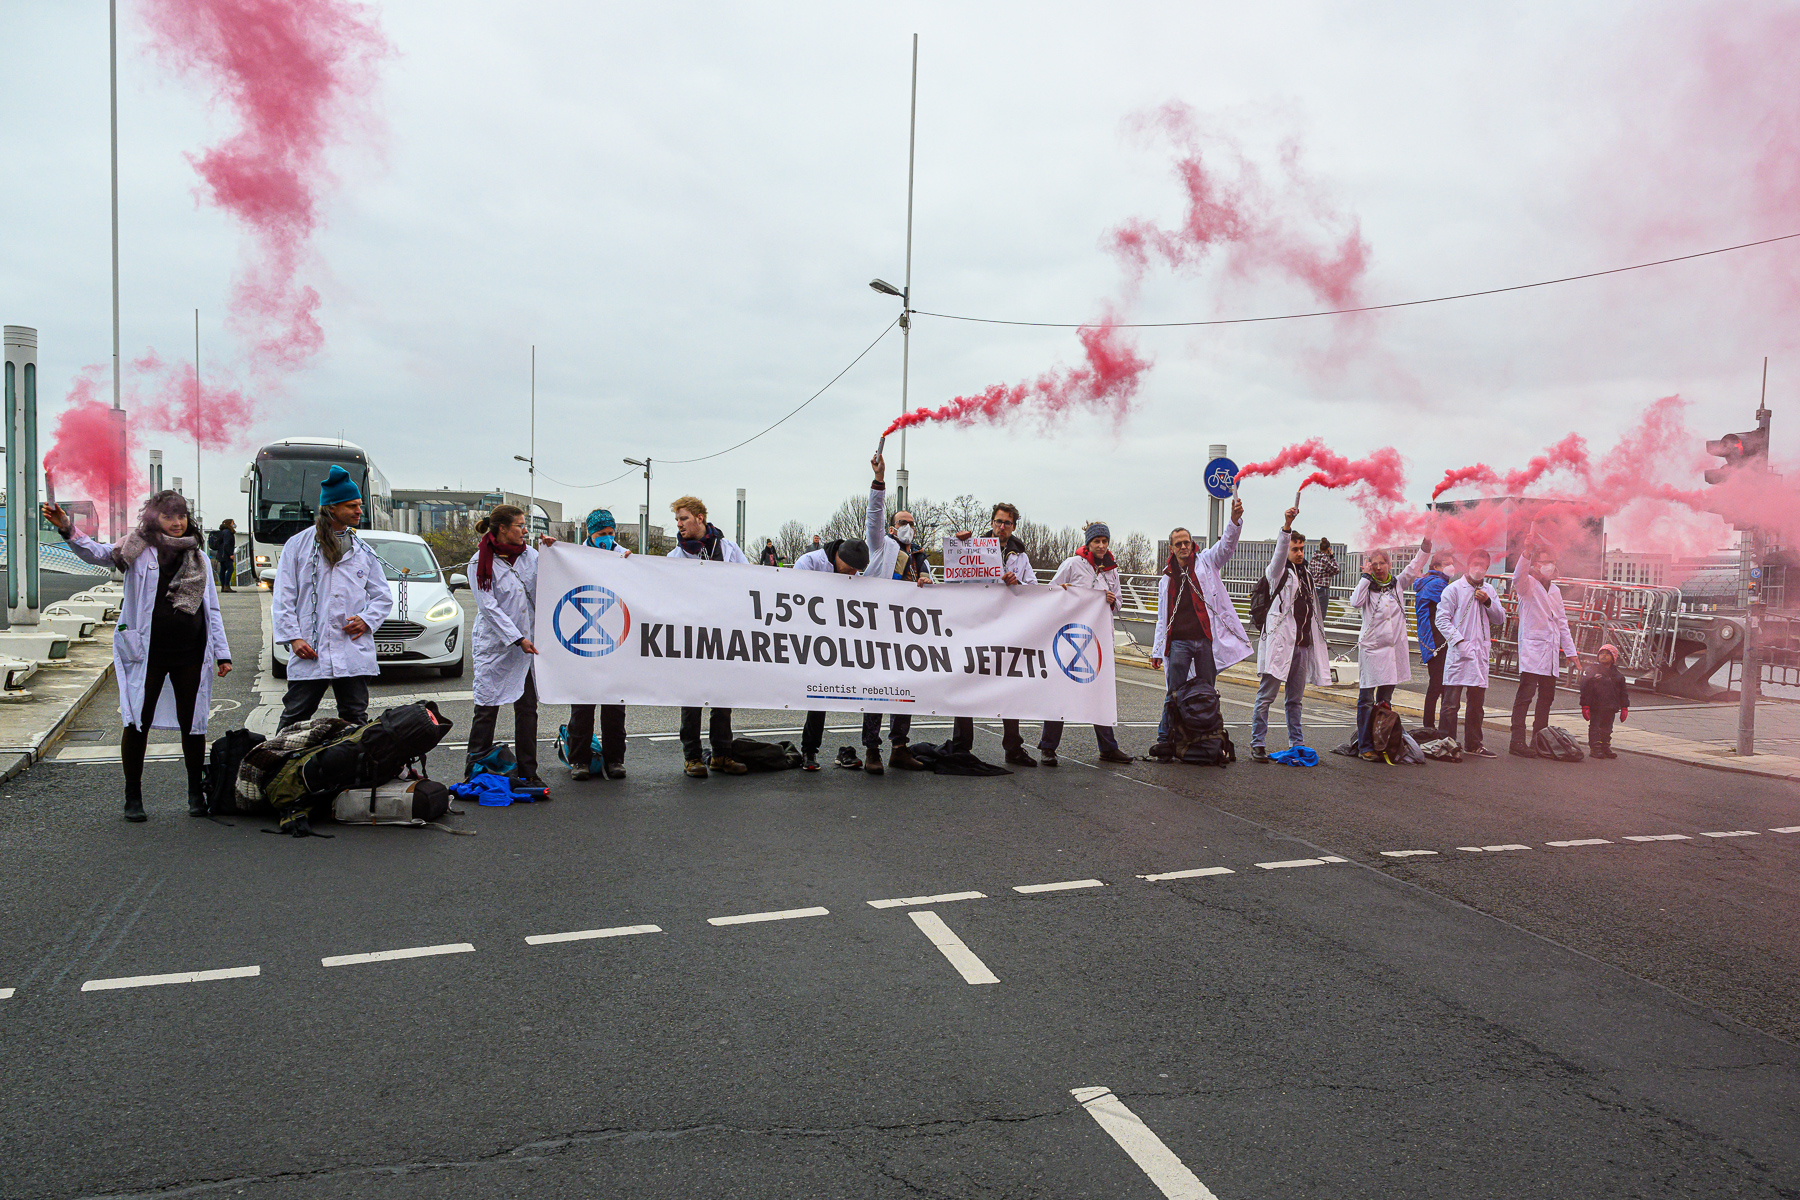
\includegraphics[width=\textwidth]{geteilte-Folien/Bilder/20220406-14-05-09.jpg}\\
\supertinycaption{% 
%Scientist Rebellion blockiert die Kronprinzenbrücke um auf Veröffentlichung IPCC-Report
%  hinzuweisen. 
Scientist Rebellion blockiert Kronprinzenbrücke in Berlin, 06.04.2022. Bild: CC-BY: Stefan Müller}
\end{column}
\begin{column}{35mm}
{\tiny
\begin{itemize}
\item[–] Andreas Zilker, Geograf,
\item[–] Anja Freiwald, Biotechnologin,
\item[–] Christian Bläul, Physiker
\item[–] Dr. Cornelia Huth, Ernährungswissenschaftlerin und Epidemologin, 
\item[–] Daniele Artico, Physiker,
%Florian Zander, 
\item[–] Friedrich Gräber, B.Sc. Biochemie,
%Harald Walsberg, Klimaaktion, Klimaschutz, 
\item[–] Kyle Topfer, Umweltwissenschaftler,
\item[–] Michael Hofmann, theoretischer Physiker,
\item[–] Dr. Nana-Maria Grüning, Biologin, 
\item[–] Prof. Dr. Nikolaus Froitzheim, Strukturgeograf,
\item[–] Dr. Stephanie Rach, Tierärztin,
\item[–] Wolfgang Metzeler-Kick, Ingenieur für technischen Umweltschutz,
\item[–] Dr. Valeria Scagliotti, Biologin,

\item[–] Seit 4/2022 internationale Proteste, auch Peter Kalmus, Klimaforscher bei NASA.

\#DontLookUp

\end{itemize}
}
\end{column}
\end{columns}

}

\frame{
\frametitlefit{Chomsky: I support the actions of the Just Stop Oil coalition}

\vfill\vfill
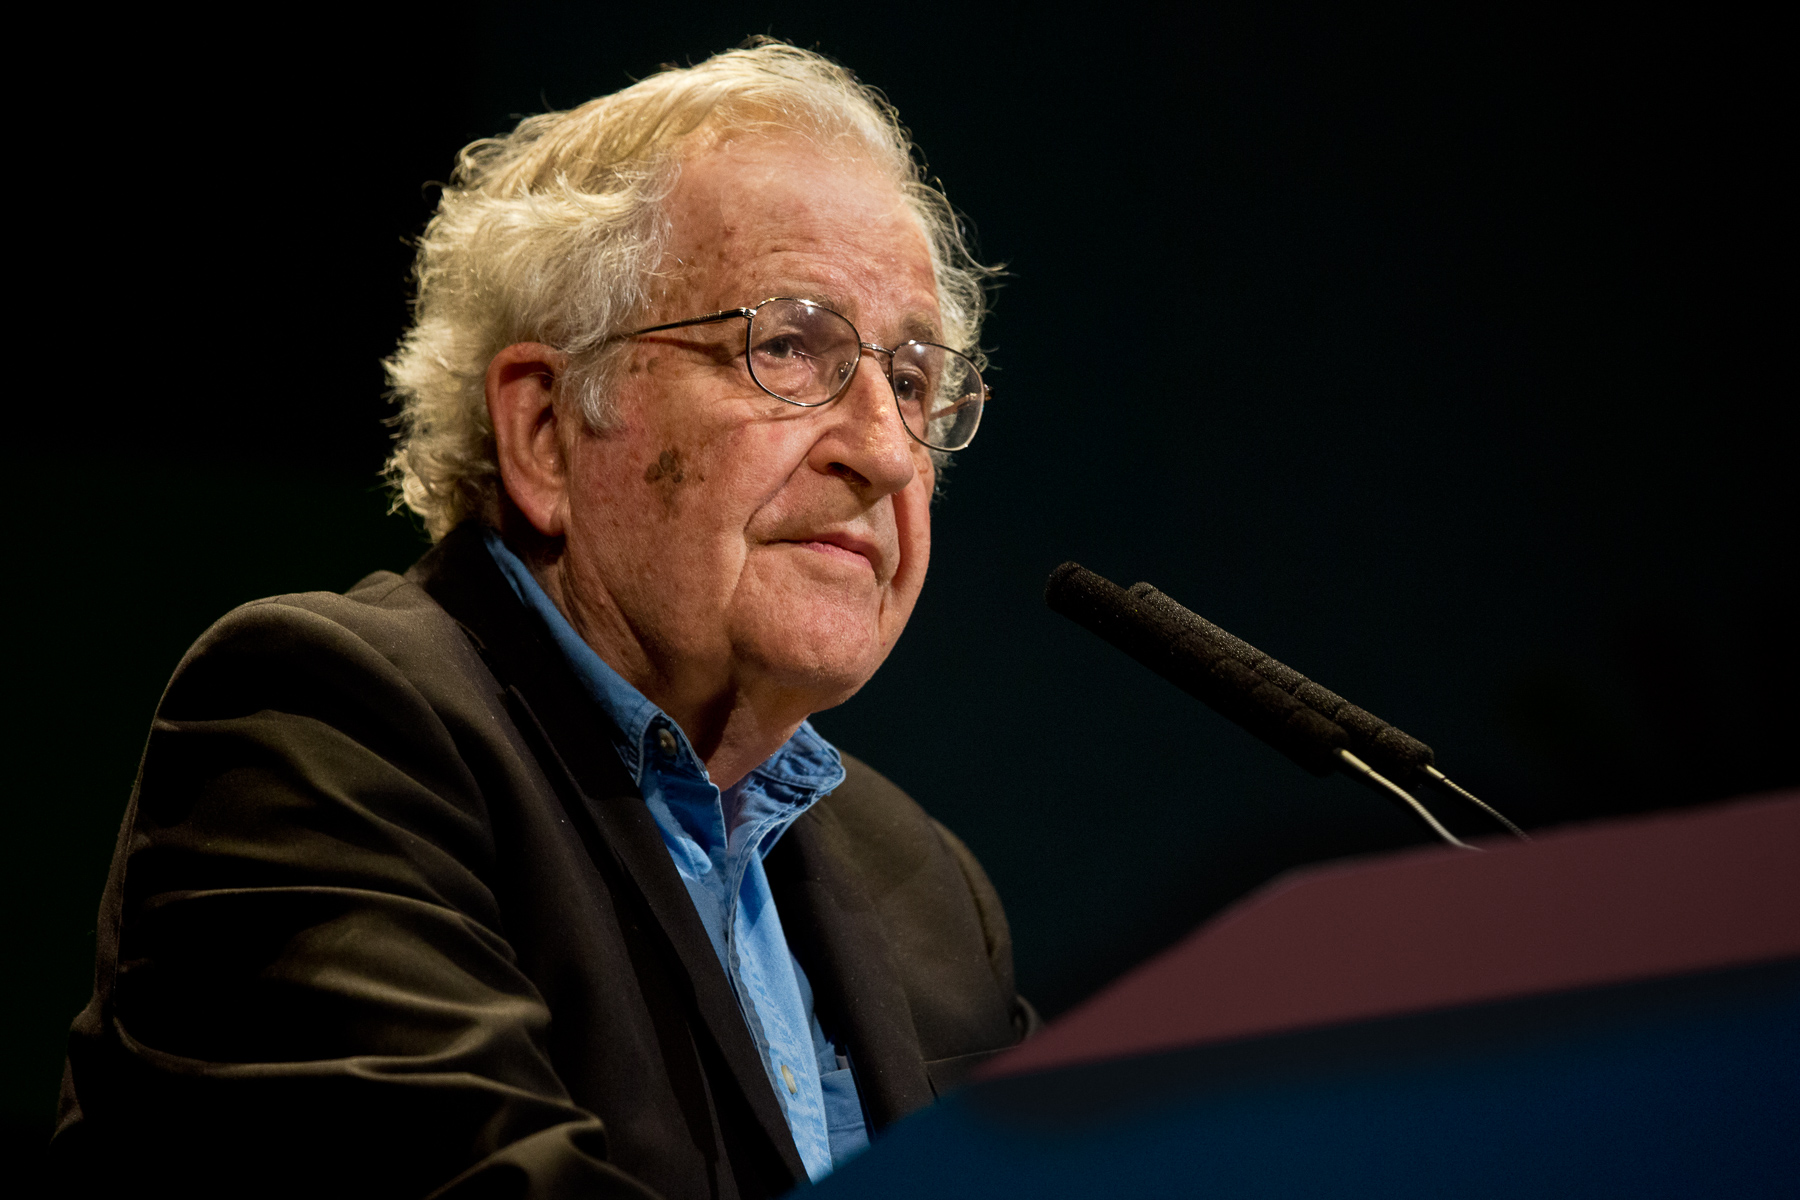
\includegraphics[width=0.65\textwidth]{geteilte-Folien/Bilder/chomsky-20150312-18-15-32.jpg}\\
\supertinycaption{% 
Noam Chomsky, 12.03.2015. Bild: CC-BY-SA: Augusto Starita}

\vfill

Video: \href{https://youtu.be/sTS04viZcGU}{Noam Chomsky on Just Stop Oil}

}

\frame{
\frametitle{Was ist Just Stop Oil? Was die Koalition?}

\begin{itemize}
\item Just Stop Oil ist eine britische Aktionsgruppe aus dem Extinction Rebellion-Umfeld.
\item Im Gegensatz zu XR blockieren sie keine Straßen, um die Politik zum Handeln aufzufordern,
sondern sie blockieren direkt relevante Infrastruktur.
\item Untertunnelung von Zufahrten zu Öl-Terminals.
\item Aus gewaltfreiem zivilem Ungehorsam ist gewaltfreier ziviler Widerstand geworden.

\bigskip

\item Was ist die Koalition?

\begin{itemize}
\item Scientist Rebellion (laut Prof. Niko Froitzheim, 13.05.2022, 1000 scientists weltweit)
\item Aufstand der Letzten Generation
\item Save old Growth (Kanada)
\item \ldots
\item Scientist Rebellion solidarisiert sich explizit mit dem Aufstand der Letzten Generation.
\end{itemize}
\end{itemize}


}

\frame[shrink=5]{
\frametitle{Katastrophenereignisse der letzten Jahre (2021--2022)}

\begin{itemize}
\item Kältewelle in den USA:
  \href{https://www.tagesschau.de/multimedia/video/video-827413.html}{Tagesschau 22.02.2021}

\item Hitze in USA/Kanada: \href{https://www.tagesschau.de/multimedia/video/video-884869.html}{Tagesschau 02.07.2021}

\item Starkregen in China (12 Tote):
  \href{https://www.tagesschau.de/multimedia/video/video-893071.html}{Tagesschau 21.07.2021} (U-Bahn)

\item Starkregen in New York (44 Tote):
  \href{https://www.tagesschau.de/multimedia/video/video-913415.html}{Tagesschau 03.09.2021}

%\item Welt: https://www.youtube.com/watch?v=msLx4ZdjUFU

\item Überflutungen Kanada (Notstand): \href{https://www.youtube.com/watch?v=3DKGoELrCN0}{Tageschau 18.11.2021}

\item Permafrostböden in der Arktis schmelzen:
  \href{https://www.mdr.de/wissen/arktis-fluesse-versiegen-rentier-eisbaer-dominoeffekt-100.html}{gute Doku im MDR}

\item Hochwasserkatastrophe in Henan, 300 Tote, 14 in U-Bahn, 200.000 evakuiert:
  \href{https://taz.de/Hochwasserkatastrophe-in-Henan/!5787142/}{taz 23.07.2021}, \href{https://www.tagesschau.de/ausland/asien/china-ueberschwemmungen-131.html}{Tagesschau 02.08.2021}



\item Antarktis 40° zu warm, Arktis 30°:
  \href{https://www.rnd.de/wissen/antarktis-temperaturen-40-grad-zu-hoch-ist-die-hitzewelle-nur-ein-aeusserst-unwahrscheinliches-3GKA6GBUIJBXHBS5OARICI2GNA.html}{rnd 22.03.2022}

\item Hunderte Millionen Menschen in Pakistan, Nord-Indien, Bangladesch  45°–48°
  \href{https://www.tagesschau.de/multimedia/video/video-1024679.html}{Tagesschau 29.04.2022},
  \href{https://www.bbc.com/news/world-asia-india-61242341}{BBC mit Film}
\end{itemize}

Is ja weit weg! Nee, isses nicht:  Ahrtal, Starkregen in Berlin 2017

30 Mrd € Schäden im Ahrtal 2021.\\
Auf Jahre Handwerker*innen beschäftigt.\\
Aber in diesem und jedem kommenden Jahr wird es neue Katastrophen geben.

Dürren. (\href{https://www.nationalgeographic.de/umwelt/2022/03/hydrologen-warnen-deutschland-trocknet-aus}{National
  Geographic, 22.03.2022})

Lieferketten gestört. 
%Teilweise durch Corona. Sich verstärkende Krisen. Und Zoonosen sind auch duch

}


\frame{
\frametitle{Folgen}

\begin{itemize}
\item Och, is doch schön, wenn's 'n bisschen wärmer wird.
\item Nee, isses nicht:\\
 Artensterben: Arten wanderen zu den Polen bzw. nach oben. 

Aber unterschiedliche Trigger:
  Temperatur bzw. Licht. 

Wenn Futter auf anderen Trigger reagiert, sterben Lebewesen aus. 

Die Ernährungskette wird löchrig. Es droht ein Kollaps. Wir sind mitten drin. (Hering in der Ostsee)

\item Regionen der Welt werden ubewohnbar. Hitze, Fluten.

\item Migration, Kriege.


\end{itemize}

}

\frame{
\frametitlefit{Prof. Dr. Maja Göpel zu existenziellen Bedrohungen der Menschheit}

\vfill
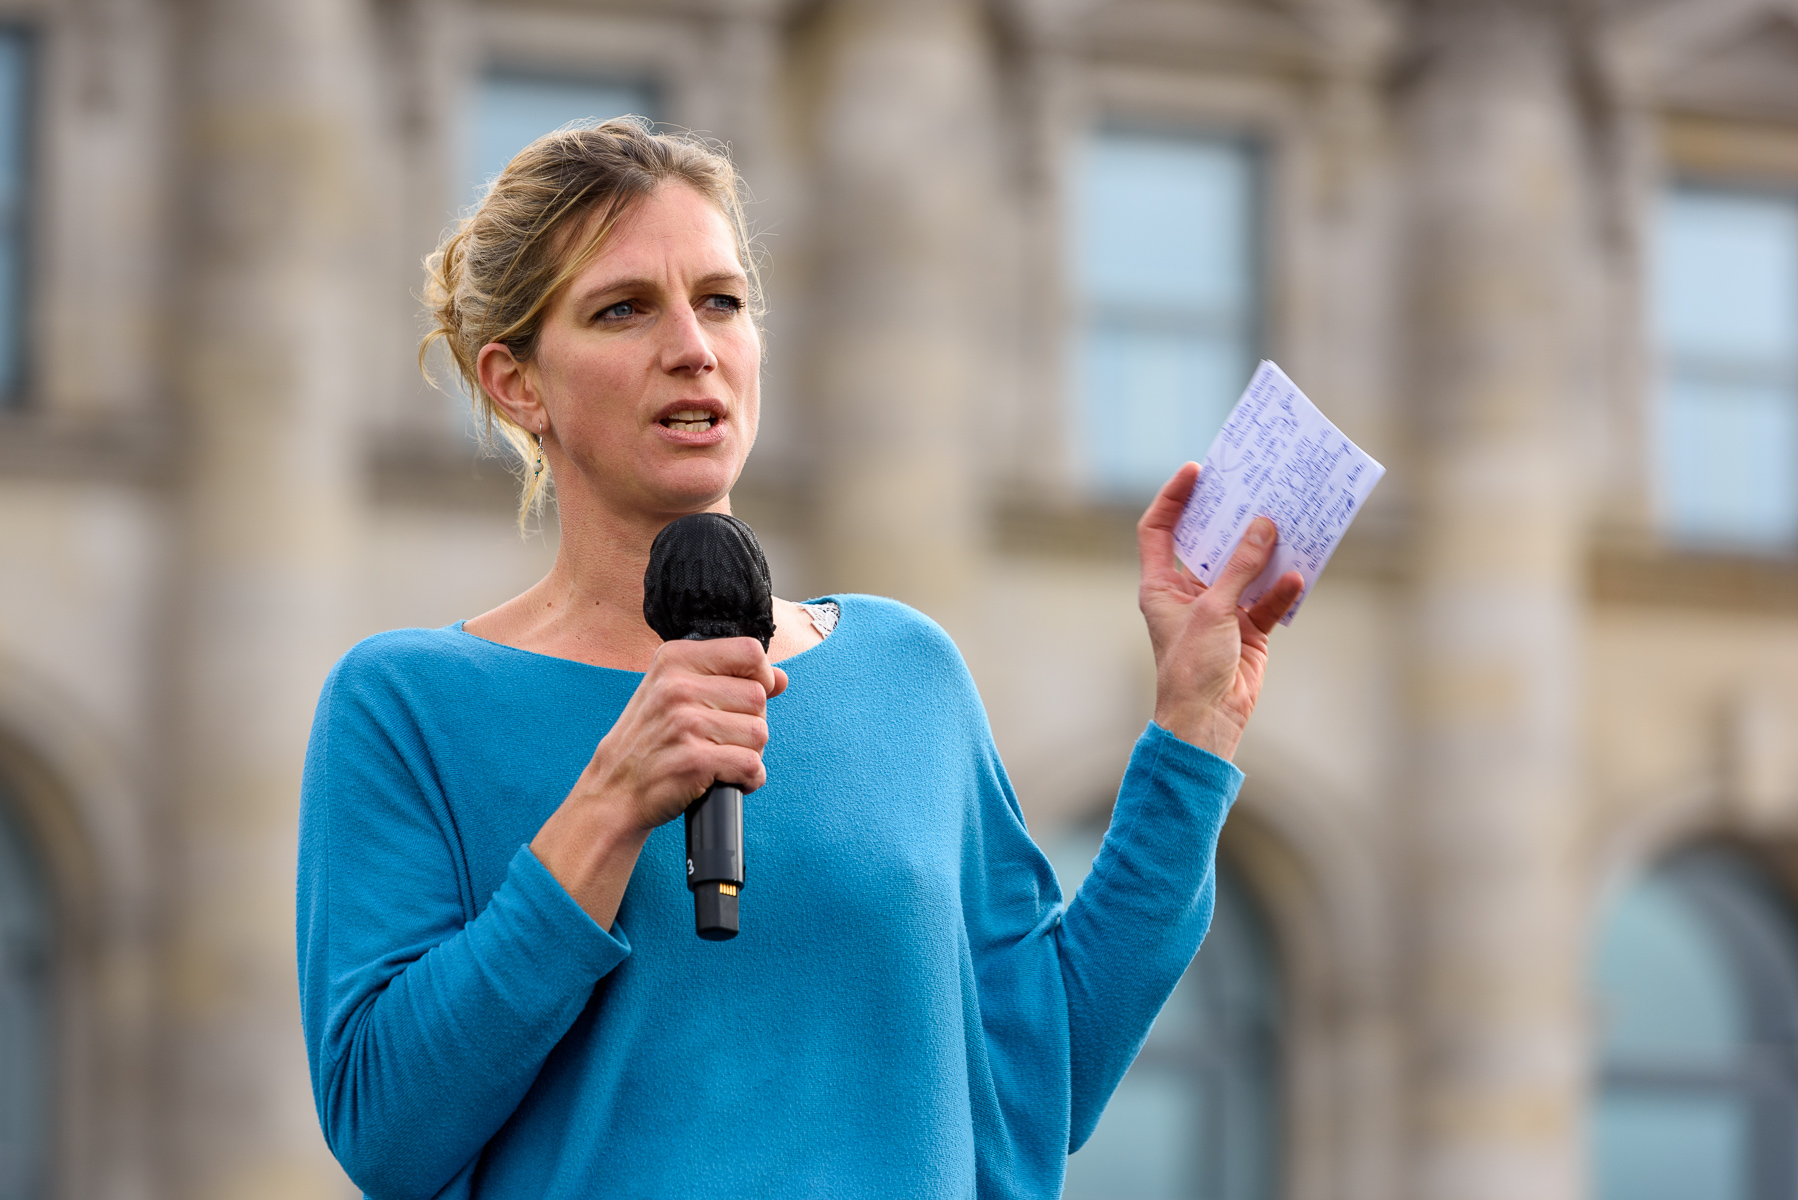
\includegraphics[width=0.65\textwidth]{geteilte-Folien/Bilder/20210924-12-39-42.jpg}\\
\supertinycaption{Maja Göpel spricht bei FFF am 24.09.2021, Bild CC-BY: Stefan Müller}
\vfill

\href{https://www.youtube.com/watch?v=Mp3z9z3Ecv4}{Video BPK}:
fünf ökologisch und die sechste Massenvernichtungswaffen
\vfill

}

\subsection{6.\ IPCC-Sachstandsbericht}

\frame{
\frametitle{Was ist los?}

\begin{itemize}
\item 6.\ IPCC-Sachstandsbericht
\item Die Lage ist verheerend. Das, was wir haben, haben wir bei 1,1° oder 1,2°. Angestrebt sind 1,5°
  also viel schlimmer. Aber so, wie wir jetzt handeln, kommen wir nicht bei 1,5° an.

\end{itemize}


}

\frame[shrink=5]{
\frametitle{CO2-Budget: Grad-Ziele, Budget und Wahrscheinlichkeiten}

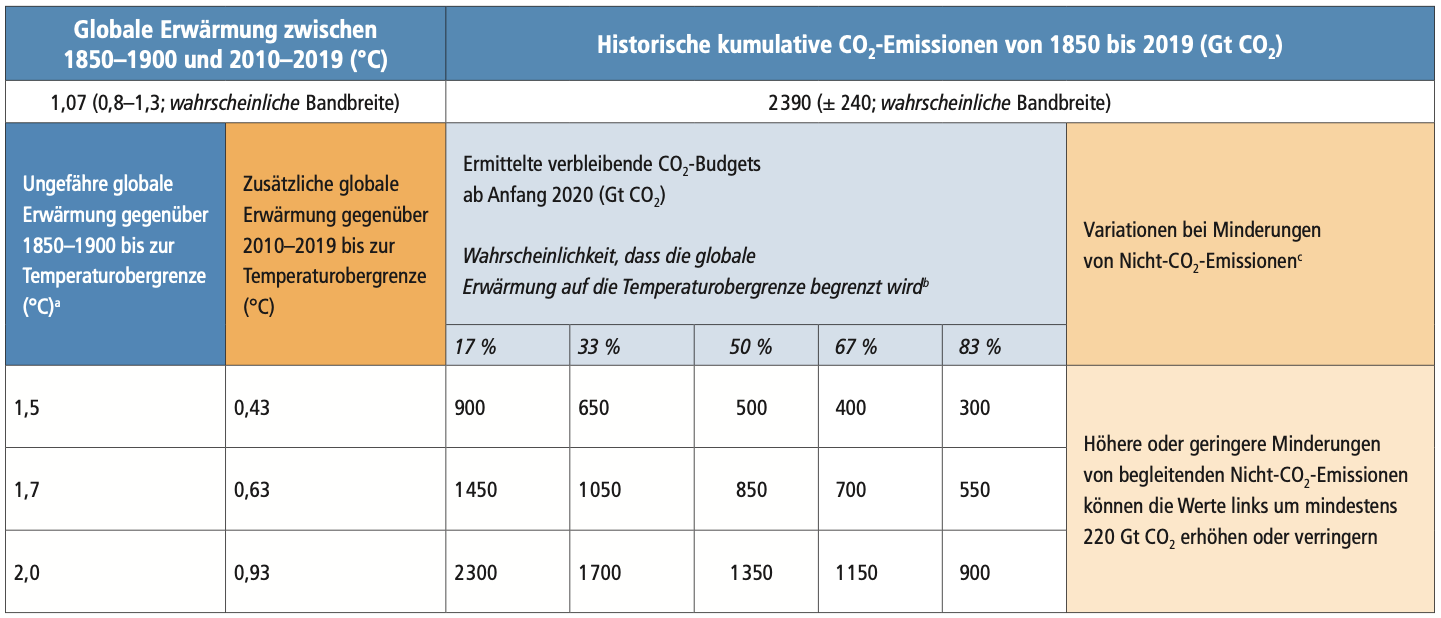
\includegraphics[width=\textwidth]{geteilte-Folien/Bilder/IPCC-CO2-Restbudget.png}\\

{\small
\begin{itemize}
\item 1,5° mit 83\,\% Wahrscheinlichkeit bedeutet ein Restbudget von 300Gt CO2.
\item Die Tabelle ist aber von Anfang 2020 \citep[\page 32]{IPCC2021-deutsch}.
\item Inzwischen haben wir weitere 70Gt CO2 emittiert.
\item Es bleiben also 230Gt für die ganze Welt.
\end{itemize}
}

}

\frame{
\frametitle{Der kleine Rest: CO2 historisch}

\begin{itemize}
\item Wie teilen wir den Rest auf? Gerecht natürlich! Aber was heißt das?
\item Es gibt fünf Verfahren für die Aufteilung \citep[\page 48]{Sachverstaendigenrat2020a}.
\item Wir setzen einfach die Zeit 1850 bis Ende CO2 an und geben allen Ländern gleiche
  Verschmutzungsrechte.
\item Upsi. Unsers ist ja schon alle. (Quelle: \href{https://www.carbonmap.org/\#Historical}{The Carbon Map})


\end{itemize}

\vfill
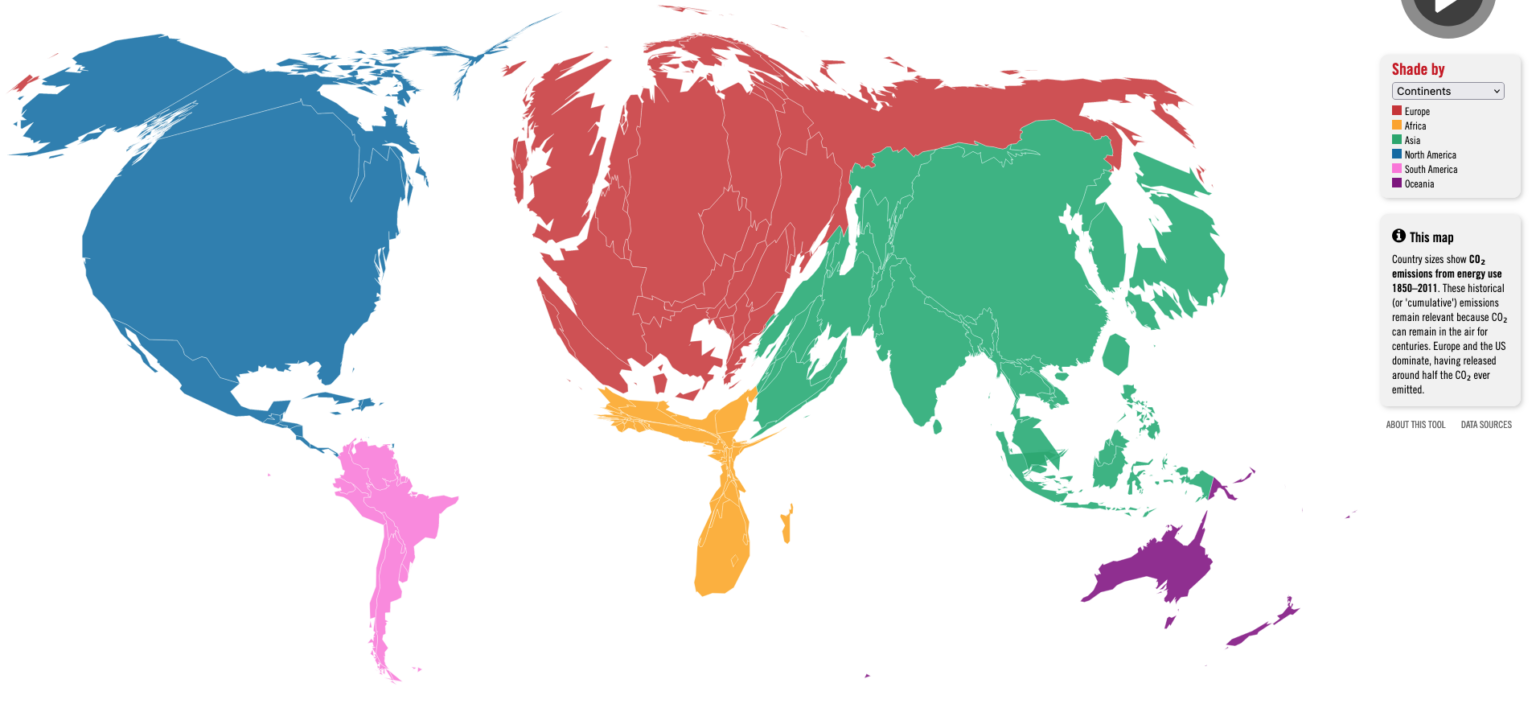
\includegraphics[width=.8\textwidth]{geteilte-Folien/Bilder/CO2-historisch.png}
\vfill

}

\frame{
\frametitle{CO2 pro lebendem Einwohner}

\begin{itemize}
\item Dann eben irgendwie anders gerecht. Wir teilen das unter den Lebenden auf.
\item D hat gegenwärtig 2\,\% des Ausstoßes, aber nur 1\,\% der Weltbevölkerung.
\item 1\,\% bedeutet 2,3 Gt für Deutschland.
\item "`Unter diesen ganzen Tonnen kann sich ja niemand etwas vorstellen."', Svenja Schulze,
  Bundesumweltministerin 2019 auf die Frage, wie hoch denn unser Restbudget wäre.
\item Was bedeutet das für jede/n Einzelnen. 2,3Gt / 83 Mio = 27,7 t.
\item Der Durchschnitts CO2-Ausstoß pro Person in Deutschland sind 9–11t pro Jahr.
\item Das heißt: In drei Jahren ist alles alle.
\end{itemize}

}

\frame{
\frametitle{Wir machen es anteilig, wie immer}

\begin{itemize}
\item Gerecht per Kopf geht ja nicht! Wir können ja nicht plötzlich, \ldots (Sarcasm)
\item Methode: grandfathering:\\
      Wir machen weiter Dreck, weil wir das schon immer gemacht haben.
\item Westen darf mehr als Entwicklungsländer. Das ist die Methode der EU.
\item Die gute Nachricht: Wir haben dann noch doppelt so lange Zeit.
\item Upsi. Sind ja auch nur sechs Jahre.

%\item Sechs Jahre = 1 freiwilliges soziales Jahr + Studium.

\bigskip

\item Nebenbemerkung: Wenn jeder sich seine Lieblingsmethode aussucht, landen wir bei
  3,2°. \citep[\page 48]{Sachverstaendigenrat2020a}


\end{itemize}


}

\frame{
\frametitle{Zur Einordnung: ein einzelnes Auto $\to$ alles weg}

\begin{itemize}
\item Autos sind in Deutschland durchschnittlich 10 Jahre zugelassen.
\item In dieser Zeit stoßen Verbrenner so viel CO2 aus, wie jeder noch übrig hat.
\item Dabei ist die Herstellung nicht berücksichtigt. Ja nach Auto 10–30t.
\item Die Herstellung fällt auch bei E-Autos an.
\item $\to$ Car is over.
\end{itemize}

\flushright\vspace{-7mm}\begin{tabular}{@{}l@{}}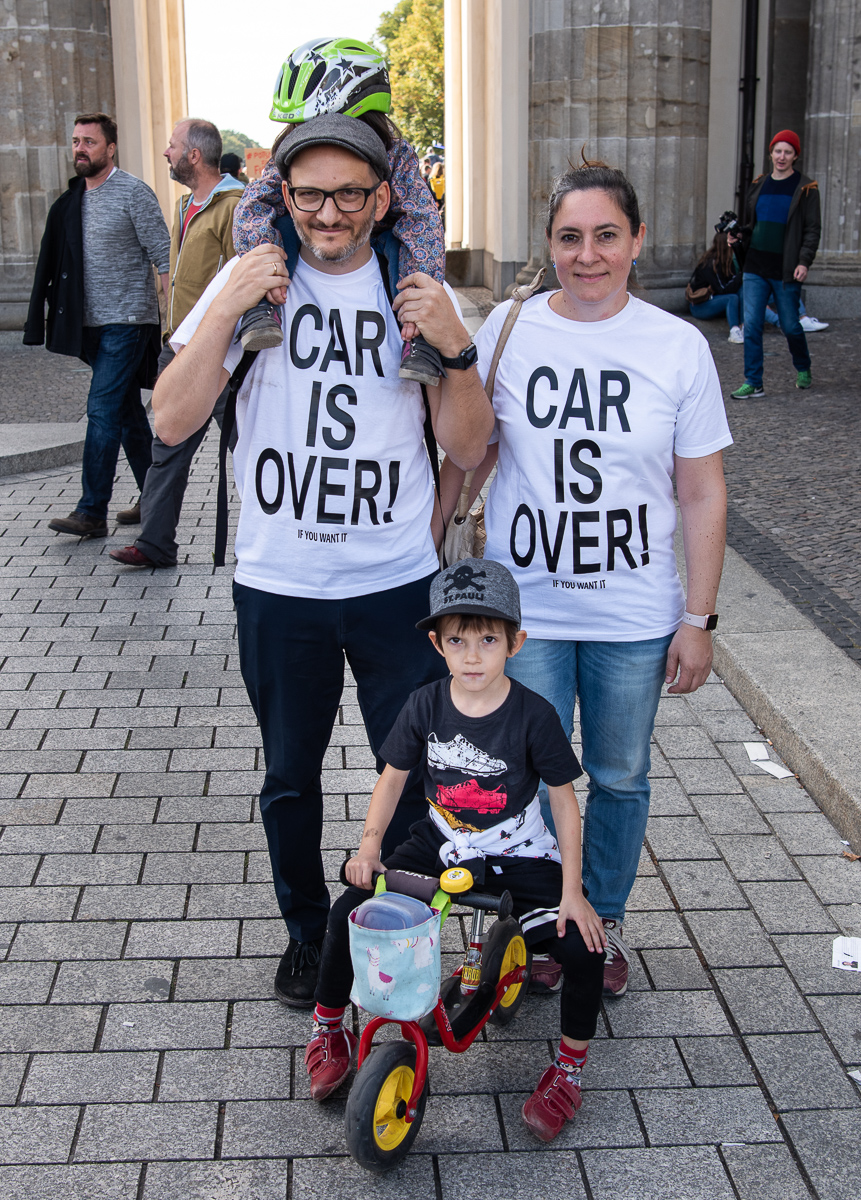
\includegraphics[width=.27\textwidth]{geteilte-Folien/Bilder/car-is-over-20190920-15-06-18.jpg}\\
\raisebox{2mm}[0pt][0pt]{\supertinycaption{Bei FFF, 20.09.2019, CC-BY St Mü}}\end{tabular}\hspace{8mm}


}


\subsection{UN-Generalsekretär António Guterres}

\frame{
\frametitle{UN-Generalsekretär António Guterres}


\begin{itemize}
\item António Guterres: \href{https://media.un.org/en/asset/k1x/k1xcijxjhp}{Link}

\item Amtliche Übersetzung auf Deutsch: \href{https://unric.org/de/ipcc280202022/}{Link}



\end{itemize}


}


\frame[shrink=5]{
\frametitlefit{Blockierer*innen hätten sich den Text nicht passender ausdenken können}

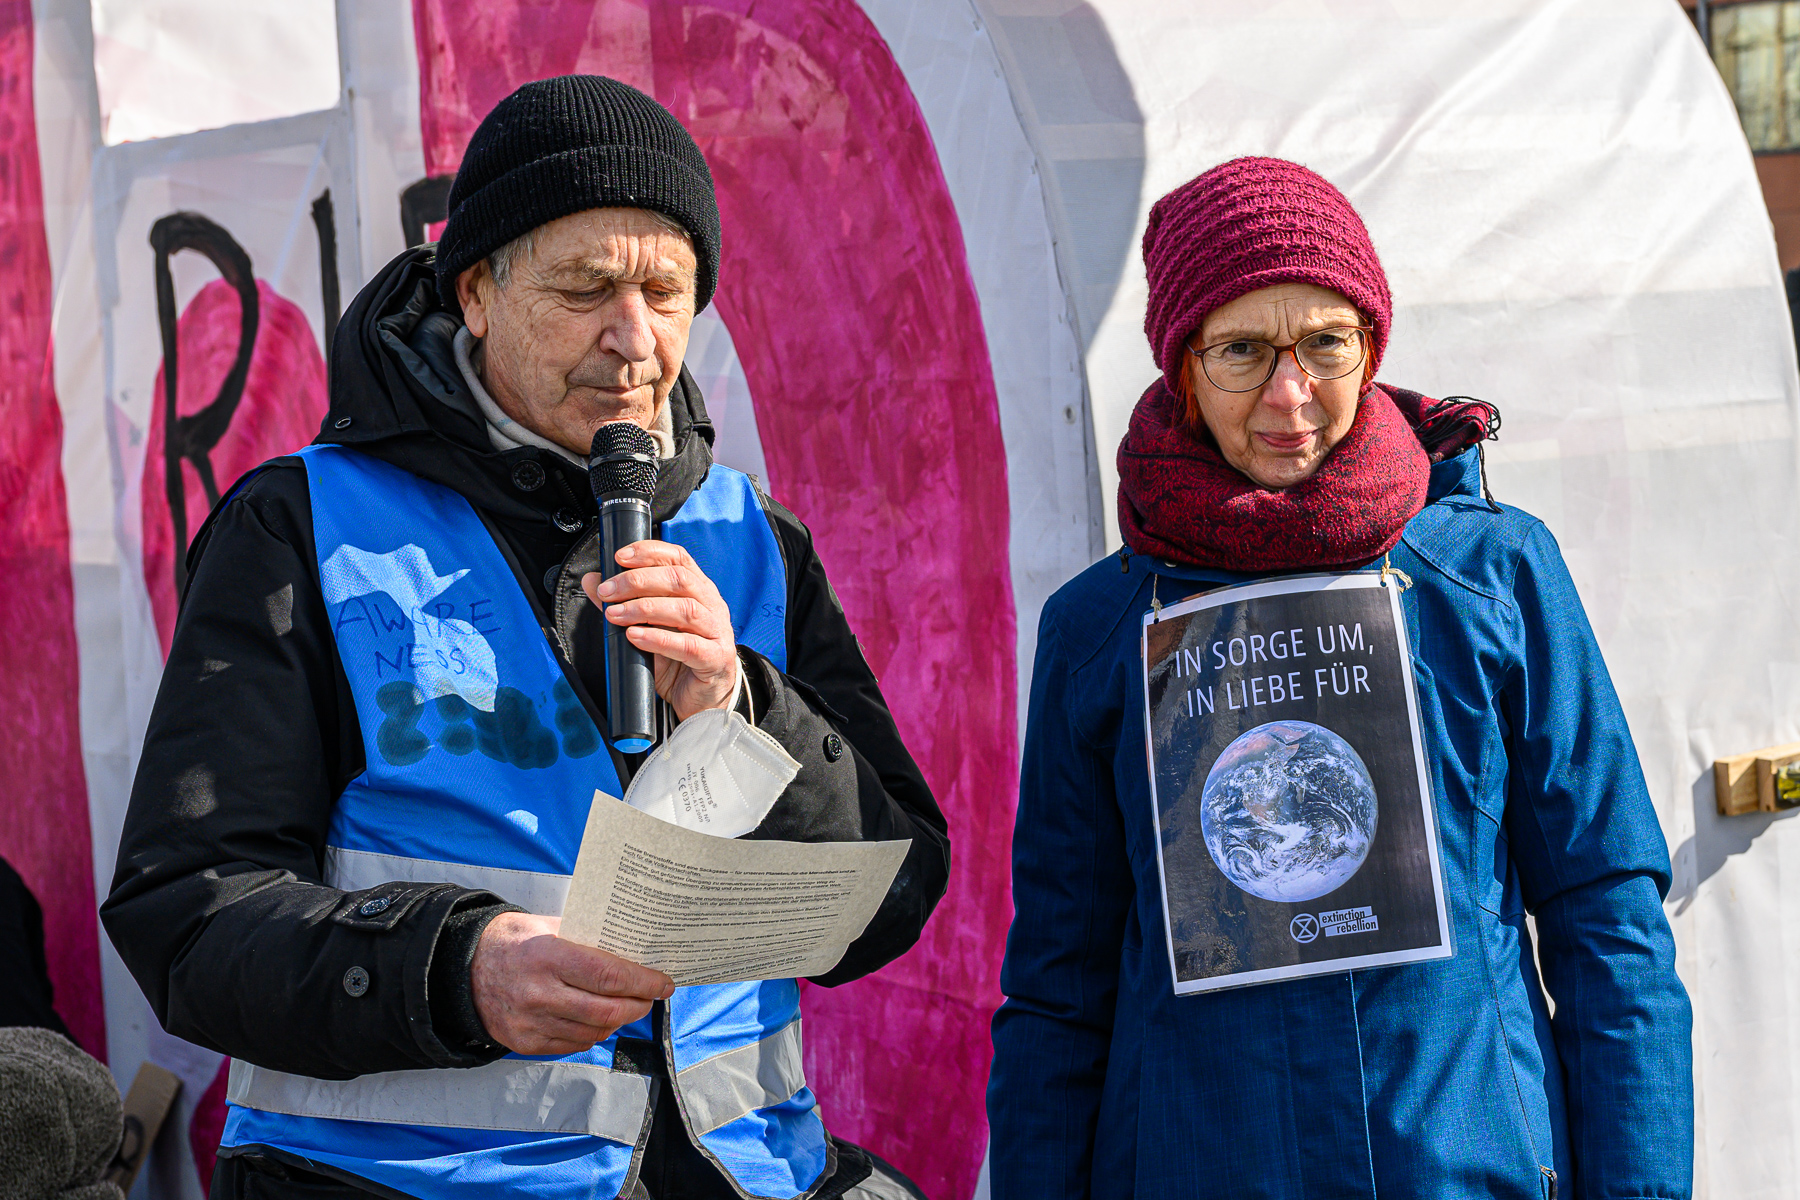
\includegraphics[width=.5\textwidth]{geteilte-Folien/Bilder/20220305-13-26-59.jpg}\\
\supertinycaption{Blockade der Marschallbrücke in Berlin durch Extinction Rebellion, 05.03.22. Bild: CC-BY Stefan Müller}

\tiny
„Die G20 müssen mit gutem Beispiel vorangehen, sonst wird die Menschheit einen noch tragischeren Preis zahlen.

Ich weiß, dass die Menschen überall ängstlich und wütend sind.

Ich bin es auch.

Jetzt ist es an der Zeit, die Wut in Taten umzusetzen.

Jeder Bruchteil eines Grades zählt.

Jede Stimme kann einen Unterschied machen.

Und jede Sekunde zählt.

Ich danke Ihnen.“ António Guterres, 28.02.2022


}




\frame[shrink=5]{
\frametitle{Was kann man selbst tun?}


Es ist schlimm, wenn man das Gefühl hat, selbst nichts tun zu können.\\
Ein bisschen kann man tun:
\begin{itemize}
\item weniger/kein Fleisch essen
\item weniger/nicht fliegen
\item In der Stadt Auto abschaffen. Sonst weniger/anders fahren.
\item weniger/anders heizen und lüften
\end{itemize}

\pause
Wichtiger sind aber die großen gesellschaftlichen Veränderungen.
\begin{itemize}
\item politisch aktiv werden/bleiben
\item Bürger*innenrat (Vertreter*innen alle Parteien wollen das inzwischen: Koalition, Schäubele,
  Köhler, \ldots)
\begin{itemize}
\item Steuern
\item Tempolimit
\item Agrarwende, Verkehrswende, Energiewende
\item usw.
\end{itemize}
\item Für all das gibt es Mehrheiten in der Bevölkerung.\\
      Klimaräte in Frankreich und Dänemark waren erfolgreich.\\
      Es gab auch in D schon einen (\href{taz, 25.06.2021}{taz, 25.06.2021})
\end{itemize}


}


\frame{
\frametitle{Was müssen wir alle gemeinsam tun?}


\begin{itemize}
\item Just stop oil! (und Kohle) "`It's now or never! Failure is not an option!"' (Chomsky, 2022)
\item Guardian: Carbon Bombs \href{https://www.theguardian.com/environment/ng-interactive/2022/may/11/fossil-fuel-carbon-bombs-climate-breakdown-oil-gas}{Link}
\item Lea Dohm (Psychologists for Future, 13.05.2022):\\ Macht, was Ihr am besten könnt,\\ was Euch Spaß
  macht.\\Macht es in der Gruppe.

\end{itemize}

}

\frame{
\frametitle{Zum Beispiel: Stadtradeln}

\begin{itemize}
\item Habe ich gerade zum Aufstand aufgerufen?
\item Ach i wo.
\item Wir machen alle Stadtradeln. In der Gruppe!
\item Das unschlagbare Linguisten-Team hat schon 27 Mitglieder.
\item Link ist im Moodle.
\end{itemize}

}

\exewidth{(35)}
\subtitle{Einleitung}

\huberlintitlepage[22pt]


%\if 0

\iftoggle{einfsprachwiss-exclude}{
\section{Motivation fromale Syntax und Phrasenstrukturgrammatiken}
}

\iftoggle{hpsgvorlesung}{

\subsection{Ziele}

\frame{
\frametitle{Ziele}


\begin{itemize}[<+->]
\item Vermittlung grundlegender Vorstellungen über deutsche Syntax
\item Gefühl für die Daten, Zusammenhänge und Komplexität
\item Einführung in Grundannahmen in der HPSG
\item Befähigung zum Schreiben formaler Grammatiken
\item Die Erleuchtung und Erlangung übernatürlicher Kräfte
\end{itemize}


}

}

\iftoggle{syntaxvorlesungen}{

\frame{
\frametitle{Alte Weisheit}

{}[Grammatik ist] das Tor zur Freiheit, die Medizin für die Krankheiten der Sprache, der Reiniger
aller Wissenschaften; sie verbreitet ihr Licht über ihnen; \ldots{} sie ist
die erste Sprosse auf der Leiter, die zur Realisierung übernatürlicher Kräfte führt und der
gerade, königliche Weg für diejenigen, die die Freiheit suchen. (Bhartrhari, Spruchdichter,
gest.\ vor 650 n. Chr., aus \emph{Vakyapadiya}, gefunden von Gabriele Knoll)

}
}

\iftoggle{hpsgvorlesung}{
\outline{

\begin{itemize}
\item Wozu Syntax? / Phrasenstrukturgrammatiken
\item Formalismus
\item Valenz und Grammatikregeln
\item Komplementation
\item Semantik
\item Adjunktion und Spezifikation
\item Das Lexikon: Typen und Lexikonregeln
\item Topologie des deutschen Satzes
\item Konstituentenreihenfolge
\item Nichtlokale Abhängigkeiten
\item Relativsätze
\item Lokalität
%\item Komplexe Prädikate: Der Verbalkomplex
\end{itemize}
}
}%\end{hpsgvorlesung}


\iftoggle{einfsprachwiss-exclude}{
\frame{
\frametitlefit{Literaturhinweise}

\begin{itemize}
\item Literatur: \citew[Kapitel~1]{MuellerLehrbuch} bzw.\ \citew[Kapitel~1]{MuellerGTBuch}
\item Englische Version des Grammatiktheoriebuches: \citew[Kapitel~1]{MuellerGT-Eng}
\end{itemize}

\vspace{1cm}

%%\rotbf{Achtung, wichtiger Hinweis: Diese Literaturangabe hier bedeutet,\\dass Sie die Literatur zum
%%   nächsten Mal lesen sollen!!!!}
%% }
}
}%\end{einfsprachwiss-exclude}


\subsection{Wozu Syntax?}



\frame{
\frametitle{Wozu Syntax?}

\begin{itemize}
\item Literatur: \citew[Kapitel~1]{MuellerLehrbuch} bzw.\ \citew[Kapitel~1]{MuellerGTBuch}
\medskip

\item Zeichen: Form-Bedeutungs-Paare \citep{Saussure16a-Fr}
\pause
\item Wörter, Wortgruppen, Sätze
\pause
\item Sprache $\stackrel{?}{=}$ endliche Aufzählung von Wortfolgen\\
\pause
      Sprache ist endlich, wenn man maximale Satzlänge annimmt
      \eal
      \ex Dieser Satz geht weiter und weiter und weiter und weiter \ldots
\pause
      \ex {}[Ein Satz ist ein Satz] ist ein Satz.
      \zl
\pause
      extrem viele Sätze, Beschränkung der Wiederholung willkürlich

\item Unterscheidung zwischen \alert{Kompetenz} (das Wissen darüber, was geht) und
  \alert{Performanz} (der Benutzung des Wissens)

\end{itemize}
}


\frame{
\frametitle{Die Kinder von Bullerbü}

Und wir beeilten uns, den Jungen zu erzählen, wir hätten von Anfang an gewußt, daß es nur eine
Erfindung von Lasse gewesen sei. Und da sagte Lasse, die Jungen hätten gewußt, daß wir gewußt
hätten, es sei nur eine Erfindung von ihm. Das war natürlich gelogen, aber vorsichtshalber sagten
wir, wir hätten gewußt, die Jungen hätten gewußt, daß wir gewußt hätten, es sei nur eine Erfindung
von Lasse. Und da sagten die Jungen -- ja -- jetzt schaffe ich es nicht mehr aufzuzählen, aber es
waren so viele "`gewußt"', daß man ganz verwirrt davon werden konnte, wenn man es hörte. (S.\,248)

\bigskip

Wir sind prinzipiell in der Lage, komplexere Sätze zu bilden (Kompetenz), aber irgendwann werden wir
verwirrt, weil unsere Gehirne nicht mehr mitmachen (Performanz).


}




\frame{
\frametitle{Kreativität}


\begin{itemize}
\item Wir können Sätze bilden, die wir noch nie gehört haben $\to$\\
      muss Strukturierung, Muster geben

\end{itemize}


}

\frame{
\frametitle{Direkte Evidenz für syntaktische Strukturen?}

\begin{itemize}
\item Wir können feststellen, dass wir Regeln verwenden,\\
      indem wir Kinder beobachten.
      
      Kinder wenden Regeln mitunter falsch an (bzw. eben ihre eigenen Regeln).

\pause
\item Beispiel aus der Morphologie:
\eal
\ex[*]{
die Baggers
}
\ex[*]{
die Ritters
}
\zl
\end{itemize}
}


\frame{
\frametitle{Wozu Syntax? Bedeutung aus Bestandteilen ermitteln}

\begin{itemize}
\item Bedeutung einer Äußerung aus den Bedeutungen ihrer Teile bestimmen
      \ea
      Der Mann kennt diese Frau.
      \z
\pause
\item Syntax: Art und Weise der Kombination, Strukturierung 
      \eal
      \ex Die Frau kennt die Mädchen.
      \ex Die Frau kennen die Mädchen.
\pause
      \ex Die Frau schläft.
      \ex Die Mädchen schlafen.
      \zl
        Subjekt-Verb-Kongruenz $\to$ Bedeutung von (\mex{0}a,b) ist eindeutig
\end{itemize}

}

\subsection{Warum formal?}
\frame[shrink=20]{
\frametitle{Warum formal?}


Precisely constructed models for linguistic structure can play an
important role, both negative and positive, in the process of discovery 
itself. By pushing a precise but inadequate formulation to
an unacceptable conclusion, we can often expose the exact source
of this inadequacy and, consequently, gain a deeper understanding
of the linguistic data. More positively, a formalized theory may 
automatically provide solutions for many problems other than those
for which it was explicitly designed. Obscure and intuition-bound
notions can neither lead to absurd conclusions nor provide new and
correct ones, and hence they fail to be useful in two important respects. 
I think that some of those linguists who have questioned
the value of precise and technical development of linguistic theory
have failed to recognize the productive potential in the method
of rigorously stating a proposed theory and applying it strictly to
linguistic material with no attempt to avoid unacceptable conclusions by ad hoc adjustments or loose formulation.
\citep[S.\,5]{Chomsky57a}


As is frequently pointed out but cannot be overemphasized, an important goal
of formalization in linguistics is to enable subsequent researchers to see the defects
of an analysis as clearly as its merits; only then can progress be made efficiently.
\citep[S.\,322]{Dowty79a}


\bigskip

\begin{itemize}
\item Was bedeutet eine Analyse genau?
\item Welche Vorhersagen macht sie?
\item Ausschluß anderer Analysen
\end{itemize}


}

% has to be set elsewhere since this file is included into the syntax vorlesung
%\exewidth{(35)}

\subsection{Konstituenz}

\subsubsection{Konstituententests}

\frame{
\frametitle{Einteilung in Einheiten}

\begin{itemize}
\item Sätze können Sätze enthalten, die Sätze enthalten, die \ldots:
\ea
dass Max glaubt, [dass Julius weiß, [dass Otto behauptet, [dass Karl vermutet, [dass Richard bestätigt,
[dass Friederike lacht]]]]]
\z

Das funktioniert wie eine Matrjoschka bzw.\ wie eine Zwiebel.

\pause

\item Genauso kann man in (\mex{1}) Wörter zu Einheiten zusammenfassen:
\ea
Alle Studenten lesen während dieser Zeit Bücher.
\z

Welche?

\end{itemize}


}

\frame{
\frametitle{Schachteln}

\oneline{%
\begin{pspicture}(0,0)(12,1.8)
     \rput[bl](0,0){%
\psset{fillstyle=solid, framearc=0.25,framesep=5pt}
\psframebox{%
\psframebox{%
       \psframebox{alle}
       \psframebox{Studenten}}
\psframebox{lesen}
\psframebox{%
       \psframebox{während}
       \psframebox{%
           \psframebox{dieser}
           \psframebox{Zeit}}}
\psframebox{Bücher}}}
%\psgrid
    \end{pspicture}}

Wir tun alle Wörter, die zusammengehören, in eine Schachtel. 

Diese Schachteln können wieder in andere Schachteln getan werden.

Im Beispiel ist intuitiv klar, was zusammengehört, aber gibt es Tests?

}


\frame{
\frametitle{Konstituenz}

Begriffe:
\begin{description}
\item[Wortfolge]  Eine beliebige linear zusammenhängende Folge von Wörtern,\\
                  die nicht unbedingt syntaktisch oder semantisch zusammengehörig sein müssen.
\item[Wortgruppe, Konstituente, Phrase] Ein Wort oder mehrere Wörter,\\
                  die eine strukturelle Einheit bilden.
\end{description}


}

\iftoggle{syntaxvorlesungen}{
\frame{
\frametitle{Konstituententests}

Welche kennen Sie?
\pause

\begin{itemize}
\item Substituierbarkeit/Pronominalisierungstest/Fragetest
\item Weglaßtest
\item Verschiebetest (Umstelltest)
\item Koordinationstest
\end{itemize}


}
}%\end{syntaxvorlesungen}


\frame{
\frametitle{Konstituententests (I)}


\begin{description}
\item[Substituierbarkeit]
        Kann man eine Wortfolge einer bestimmten
	Kategorie in einem Satz gegen eine andere Wortfolge so austauschen, dass
	wieder ein akzeptabler Satz entsteht, so ist das ein Indiz dafür, dass 
	die beiden Wortfolgen Konstituenten bilden.
        \eal
        \ex Er kennt den Mann.
        \ex Er kennt eine Frau.
        \zl
\pause
\item[Pronominalisierungstest]
        Alles, worauf man sich mit einem Pronomen beziehen
	kann, ist eine Konstituente.
        \eal
        \ex Der Mann schläft.
        \ex Er schläft.
        \zl
%
\end{description}

}

\frame{
\frametitle{Konstituententests (II)}

\begin{description}
\item[Fragetest]
        Was sich erfragen läßt, ist eine Konstituente.
        \eal
        \ex Der Mann arbeitet.
        \ex Wer arbeitet?
        \zl
\pause
\item[Verschiebetest] Wortfolgen, die man ohne Beeinträchtigung der
	Korrektheit des Satzes verschieben bzw.\ umstellen kann, bilden eine Konstituente.
        \eal
        \ex weil keiner diese Frau kennt.
        \ex weil diese Frau keiner kennt.
        \zl
\pause
\item[Koordinationstest]
        Was sich koordinieren läßt, ist eine Konstituente.
        \ea
        Der Mann und die Frau arbeiten.
        \z
\end{description}

}



\iftoggle{konstituentenprobleme}{
\subsubsection{Bemerkungen zum Status der Tests}

\frame{
\frametitle{Bemerkungen zum Status der Tests: Expletiva (I)}

Was ist mit \emph{es} in (\mex{1})?
\ea
Es regnet.
\z
\pause

Substituierbarkeit und Fragetest schlagen fehl:
\eal
\ex[*]{
Der Mann/er regnet.
}
\ex[*]{
Wer/was regent?
}
\zl
Aus denselben Gründen schlägt der Koordinationstest fehl:
\ea[*]{
Es und der Mann regnet.
}
\z

}


\frame{
\frametitle{Bemerkungen zum Status der Tests: Expletiva (II)}

Nur die (allerdings eingeschränkte) Umstellbarkeit ist gegeben:
\eal
\ex[]{
Es regnet.
}
\ex[]{
Regnet es?
}
\ex[]{
weil es jetzt regnet
}
\ex[*]{
weil jetzt es regnet
}
\zl
\eal
\ex[]{
Er sah es regnen.
}
\ex[*]{
Es sah er regnen.
}
\zl

\pause
Daraus folgt: Nicht alle Tests müssen positiv ausfallen,\\
damit eine Wortfolge als Konstituente gelten kann,\\
\dash, die Test stellen keine notwendige Bedingung dar.


}


\frame[shrink=10]{
\frametitle{Bemerkungen zum Status der Tests: Koordination}

%\judgewidth{?*}
\smallframe
Was ist mit \emph{der Mann einen Esel} und \emph{die Frau ein Pferd} in (\mex{1})?
\ea
Deshalb kaufte der Mann einen Esel und die Frau ein Pferd.
\z
\pause

Diese Wörter kann man nur sehr bedingt gemeinsam umstellen:
\ea[?*]{
Der Mann einen Esel kaufte deshalb.
}
\z

Ein Ersetzung durch Pronomina ist nicht ohne Ellipse möglich:
\eal
\ex[\#]{
Deshalb kaufte er.
}
\ex[*]{
Deshalb kaufte ihn.
}
\zl
Die Pronomina stehen nicht für beide logischen Argumente % von \emph{kaufen},
sondern nur für jeweils eins.

\pause
Daraus folgt: Auch wenn einige Tests erfüllt sind,\\
muß es noch lange nicht sinnvoll sein, eine Wortfolge als Konstituente einzustufen,\\
\dash, die Test stellen keine hinreichende Bedingung dar.

}

\frame{
\frametitle{Bemerkungen zum Status der Tests: Voranstellung (I)}
%
\savespace\smallexamples

Normalerweise steht im Deutschen eine Konstituente vor dem Finitum.

{\judgewidth{?*}
\eal
\ex[]{
[Alle Studenten] lesen während der vorlesungsfreien Zeit Bücher.
}
\ex[]{
[Bücher] lesen alle Studenten während der vorlesungsfreien Zeit.
}
\ex[*]{
[Alle Studenten] [Bücher] lesen während der vorlesungsfreien Zeit.
}
\ex[*]{
[Bücher] [alle Studenten] lesen während der vorlesungsfreien Zeit.
}
\zl
}

Voranstellbarkeit vor das finite Verb wird in manchen Definitionen sogar
zum ausschlaggebenden Kriterium für \textit{Satzglied} \citep[S.\,783]{Duden2005}.
}

\frame{
\frametitle{Bemerkungen zum Status der Tests: Voranstellung (II)}

%\begin{tabular}{@{p{0.95\linewidth}}
\alert{Satzgliedtest} [Auch: Konsituententest]. Auf der $\to$ Topikalisierung
beruhendes Verfahren zur Analyse komplexer Konstituenten. Da bei Topikalisierung
jeweils nur eine Konstituente bzw.\ ein $\to$ Satzglied an den Anfang gerückt werden kann,
lassen sich komplexe Abfolgen von Konstituenten (\zb Adverbialphrasen) als
ein oder mehrere Satzglieder ausweisen; in \textit{Ein Taxi quält sich im Schrittempo
durch den Verkehr} sind \textit{im Schrittempo} und \textit{durch den Verkehr}
zwei Satzglieder, da sie beide unabhängig voneinander in Anfangsposition gerückt werden
können. \citep[S.\,446]{Bussmann83a}
%\end{tabular}

\bigskip
nicht mehr enthalten in \citew{Bussmann90a}

}

\frame{
\frametitle{Bemerkungen zum Status der Tests: Voranstellung (III)}


Nach Bußmann:
\begin{itemize}
\item Teile des Materials können einzeln vorangestellt werden. $\to$\\
      Das Material bildet keine Konstituente.
\item Material kann zusammen vorangestellt werden. $\to$\\
      Das Material bildet eine Konstituente.
\end{itemize}

Beide Implikationen sind problematisch.

Die erste ist wegen Beispielen wie (\mex{1}) problematisch:
\eal
\ex \rot{Keine Einigung} \blau{erreichten} Schröder und Chirac \gruen{über den Abbau der Agrarsubventionen}. (tagesschau, 15.10.2002, 20:00)
\ex \gruen{Über den Abbau der Agrarsubventionen} \blau{erreichten} Schröder und Chirac \rot{keine Einigung}.
\zl

}

\frame{
\frametitle{Bemerkungen zum Status der Tests: Voranstellung (IV)}

Obwohl Teile der NP einzeln vorangestellt werden können,
wollen wir die Wortfolge als eine NP analysieren, wenn sie nicht vorangestellt ist.
\ea
Schröder und Chirac \blau{erreichten} \rot{keine Einigung} \gruen{über den Abbau der Agrarsubventionen}.
\z
\pause
Diese Wortgruppe kann auch gemeinsam vorangestellt werden:
\ea
\rot{Keine Einigung} \gruen{über den Abbau der Agrarsubventionen} \blau{erreichten} Schröder und Chirac.
\z

\emph{Keine Einigung über den Abbau der Agrarsubventionen} ist eine Konstituente, 
die unter gewissen Umständen aufgespalten werden kann. 

Bei Aufspaltung können die einzelnen Teilkonstituenten unabhängig voneinander umgestellt werden.

}

\frame{
\frametitle{Bemerkungen zum Status der Tests: Voranstellung (V)}

\small
\savespace
\smallexamples
Der zweite Teil des Konstituententests ist ebenfalls problematisch:


\eal
\ex {}[Dauerhaft] [mehr Arbeitsplätze] gebe es erst, wenn sich eine Wachstumsrate von
      mindestens 2,5 Prozent über einen Zeitraum von drei oder vier Jahren halten lasse. (taz, 19.04.2000, S.\,5)
\ex {}[Wenig] [mit Sprachgeschichte] hat der dritte Beitrag in dieser Rubrik zu tun, [\ldots]
    (ZS für Dialektologie und Linguistik, LXIX, 3/2002, S.\,339)
\zl


Mehr Daten in \citew{Mueller2003b}.

Wörter vor Finitum stehen werder in semantischer noch in syntaktischer Beziehung zueinander
$\to$ nicht sinnvoll, sie als eine Konstituente zu analysieren

\medskip
Die Daten kann man mit einem leeren verbalen Kopf im Vorfeld analysieren,\\
so dass letztendlich wieder V2-Strukturen vorliegen \citep{Mueller2005d}.\\
Trotzdem sind die Daten für Konstituententests problematisch.

Voranstellbarkeit ist nicht hinreichend für Konstituentenstatus.

}

\frame{
\frametitle{Bemerkungen zum Status der Tests: Voranstellung (VI)}

\judgewidth{\#}
\eal
\ex[]{
Er bringt es bis zum Professor.
}
\ex[\#]{
Es bringt er zum Professor.
} 
\zl

\emph{es} ist Konstituente, obwohl es nicht vorangestellt werden kann.

\pause
Genauso:
\eal
\ex[]{
Karl hat sich nicht erholt.
}
\ex[*]{
Sich hat Karl nicht erholt.
}
\zl

\eal
\ex[]{
Er hörte es regnen.
}
\ex[*]{
Es hörte er regnen.
}
\zl

$\to$ Voranstellbarkeit ist nicht notwendig.

Also: Voranstellbarkeit ist weder hinreichend noch notwendig.

}
}%\end{konstituentenprobleme}


\iftoggle{konstituentenprobleme-hinweis}{

\frame{
\frametitle{Warnung}


Achtung: Diese Tests liefern leider nur Indizien für den Konstituentenstatus. 

Zu den Details siehe 
%\citew[Kapitel~1.3.2]{MuellerLehrbuch3}
\citew[Abschnitt~1.3.2]{MuellerGTBuch}.
}

}%\end{konstituentenprobleme-hinweis}

\subsection{Köpfe}



\frame{
\frametitle{Köpfe}

Kopf bestimmt die wichtigsten Eigenschaften einer Phrase
\eal
\ex \alert{Träumt} er?
\ex \alert{Erwartet} er einen dreiprozentigen Anstieg?
\ex \alert{in} diesem Haus
\ex ein \alert{Mann}
\zl

\pause
Kombination eines Kopfes mit anderem Material wird
\alert{Projektion des Kopfes} genannt.

\pause
Eine vollständige Projektion ist eine \alert{Maximalprojektion}.

\pause
Ein Satz ist die Maximalprojektion eines finiten Verbs.
}

\frame{
\frametitle{Beschriftete Schachteln}

\medskip

\centerline{%
\begin{pspicture}(0,0)(7.8,3.4)
     \rput[bl](0,0){%
\psset{fillstyle=solid, framearc=0.25,framesep=5pt}
\psframebox{%
\begin{tabular}{@{}l@{}}
VP\\
\psframebox{%
\begin{tabular}{@{}l@{}}
NP\\[2mm]
       \psframebox{\begin{tabular}{@{}l@{}}
                   Det\\der
                   \end{tabular}}
       \psframebox{\begin{tabular}{@{}l@{}}
                   N\\Mann
                   \end{tabular}}
\end{tabular}}
\psframebox{\begin{tabular}{@{}l@{}}
                   V\\liest
                   \end{tabular}}
\psframebox{%
\begin{tabular}{@{}l@{}}
NP\\[2mm]
           \psframebox{\begin{tabular}{@{}l@{}}
                   Det\\einen
                   \end{tabular}}
           \psframebox{\begin{tabular}{@{}l@{}}
                   N\\Aufsatz
                   \end{tabular}}
\end{tabular}}
\end{tabular}}}
%\psgrid
    \end{pspicture}}


Wer schon einmal umgezogen ist, weiß, dass es sinnvoll ist,\\
Schachteln zu beschriften.

Im obigen Bild steht auf jeder Schachtel etwas über das wichtigste Element in der Schachtel.

}

\frame[shrink=15]{
\frametitle{Schachteln sind austauschbar}


\begin{itemize}
\item Der genaue Inhalt einer Schachtel ist egal:
\eal
\ex er
\ex der Mann
\ex der Mann aus Stuttgart
\ex der Mann aus Stuttgart, den wir kennen
\zl
Wichtig ist: Die Wörter bzw.\ Wortfolgen in (\mex{0}) sind alle nominal und vollständig: NP.

Man kann sie innerhalb größerer Schachtel gegeneinander vertauschen.

\pause
\item Das geht aber nicht mit allen NPen:

\eal
\ex[]{ 
Der Mann liest einen Aufsatz.  
} 
\ex[*]{ 
Die Männer liest einen Aufsatz.  
} 
\ex[*]{ Des Mannes liest einen Aufsatz.  
} 
\zl 

\item Es gibt Eigenschaften, die für die Verteilung (Distribution) von Phrasen wichtig sind.


\end{itemize}


}

\frame{
\frametitle{Ausführlich beschriftete Schachteln}

~\medskip

\oneline{%
\begin{pspicture}(0,0)(16.4,3.4)
     \rput[bl](0,0){%
\psset{fillstyle=solid, framearc=0.25,framesep=5pt}
\psframebox{%
\begin{tabular}{@{}l@{}}
VP, fin\\[2mm]
\psframebox{%
\begin{tabular}{@{}l@{}}
NP, nom, 3, sg, mas\\[2mm]
       \psframebox{\begin{tabular}{@{}l@{}}
                   Det, nom, sg, mas\\der
                   \end{tabular}}
       \psframebox{\begin{tabular}{@{}l@{}}
                   N, nom, sg, mas\\Mann
                   \end{tabular}}
\end{tabular}}
\psframebox{\begin{tabular}{@{}l@{}}
                   V, fin, 3, sg\\liest
                   \end{tabular}}
\psframebox{%
\begin{tabular}{@{}l@{}}
NP, akk, 3, sg, mas\\[2mm]
           \psframebox{\begin{tabular}{@{}l@{}}
                   Det, akk, sg, mas\\einen
                   \end{tabular}}
           \psframebox{\begin{tabular}{@{}l@{}}
                   N, akk, sg, mas\\Aufsatz
                   \end{tabular}}
\end{tabular}}
\end{tabular}}}
%\psgrid
    \end{pspicture}}

Alle Merkmale, die für die Distribution der gesamten Phrase wichtig sind, werden projiziert.

Diese Merkmale werden auch \alert{Kopfmerkmale} genannt.

}


% \frame[shrink=10]{
% \frametitle{Projizierte Merkmale}


% \hfill%
% \begin{tabular}{|l|l|}\hline
% Kategorie    & projizierte Merkmale\\\hline
% Verb         & Kategorie, Verbform ({\it fin\/}, {\it bse\/}, \ldots)\\
% Nomen        & Kategorie, Kasus ({\it nom\/}, {\it gen\/}, {\it dat\/}, {\it acc\/})\\
% %Präposition  & Kategorie, Form der Präposition ({\it an\/}, {\it auf\/}, \ldots)\\
% Adjektiv     & Kategorie, bei flektierten Formen Kasus\\\hline
% \end{tabular}\hfill\hfill\mbox{}
% \pause
% ~
% \bigskip

% Beispiel:
% Wenn \emph{stolzer} den Kasus Genitiv hat,\\
% dann hat auch die gesamte Adjektiv-Phrase Genitiv. 

% \ea
% \emph<3>{einiger \emph<2>{auf ihren Sohn \blau<2>{stolzer}} \blau<3>{Männer}}
% \z

% Das ist wichtig, da die Adjektiv-Phrase mit dem Determinierer und\\
% dem Nomen im Kasus übereinstimmen muß.

% \pause
% Wenn \emph{Männern} in (\mex{1}) Dativ ist, hat die gesamte NP diese Eigenschaft.
% \ea
% den Männern
% \z

% }

%\fi

\subsection{Argumente und Adjunkte}

\frame[shrink=10]{
\frametitle{Argumente}

\begin{itemize}
\item Konstituenten stehen in verschiedenartigen Beziehungen zu ihrem Kopf.
\pause
\item Man unterscheidet zwischen \alert{Argumenten} und \alert{Adjunkten}.
\pause
\item Bestimmte Mitspieler (Aktanten) gehören zur Bedeutung eines Verbs.

\ZB gibt es in Situationen, die durch \emph{lieben} beschrieben werden,\\
immer einen \emph{Liebenden} und einen \emph{Geliebten} / etwas \emph{Geliebtes}.

\eal
\ex Conny liebt Aicke.
\ex $lieben'(Conny', Aicke')$
\zl

(\mex{0}b) ist eine logische Repräsentation für (\mex{0}a).

\relation{Conny} und \relation{Aicke} sind \alert{logische Argumente} von \relation{lieben}.

\pause
\item Syntaktische Argumente entsprechen meistens den logischen (später mehr).
\pause
\item Solche Beziehungen zwischen Kopf und Argumenten werden mit dem Begriff
\alert{Selektion} bzw.\ \alert{Valenz} erfasst.
\pause
\item \citet{Tesniere59a-u} überträgt Valenzbegriff aus der Chemie auf die Linguistik.
\end{itemize}

}


%\BackgroundPicture{periodensystem}{1}{1}
\frame{
\frametitle{Valenz in der Chemie}

\begin{itemize}
\item Atome können sich mit anderen Atomen zu mehr oder weniger stabilen Molekülen verbinden. 

\pause
\item Wichtig für die Stabilität ist, wie Elektronenschalen besetzt sind. 

\pause
\item Eine Verbindung mit anderen Atomen kann dazu führen,\\
dass eine Elektronenschale voll besetzt ist,\\
was dann zu einer stabilen Verbindung führt.

\pause
\item Die Valenz sagt etwas über die Anzahl der Wasserstoffatome aus,\\
die mit einem Atom eines Elements verbunden werden können. 

\pause
\item Sauerstoff hat die Valenz 2 und kann sich zu H$_2$O verbinden.

\pause
\item Man kann nun die Elemente in Valenzklassen einteilen.\\
Elemente mit einer bestimmten Valenz werden im Periodensystem von Mendeleev
in einer Spalte repräsentiert.

\end{itemize}

}

\frame{
\frametitle{Valenz in der Linguistik}

\begin{itemize}
\item Ein Kopf braucht bestimmte Argumente,\\
      um eine stabile Verbindung einzugehen. 
\item Wörter mit der gleichen Valenz (mit gleicher Anzahl und Art von Argumenten)  werden in Valenzklassen eingeordnet, da sie sich in bezug
auf die Verbindungen, die sie eingehen, gleich verhalten. 


\bigskip

\centerline{
\begin{forest}
[O
  [H] 
  [H] ]
\end{forest}
\hspace{5em}
\begin{forest}
[lieben
 [Conny]
 [Aicke] ]
\end{forest}
}

\bigskip

Verbindung von Sauerstoff mit Wasserstoff und Verbindung
eines Verbs mit seinen Argumenten

\end{itemize}

\vfill

}

\frame{
\frametitle{Optionale Argumente}

\begin{itemize}
\item Argumente müssen nicht immer realisiert werden:
\eal
\ex Er wartet auf den Installateur.
\ex Er wartet.
\zl
\pause
Das Präpositionalobjekt von \emph{warten} 
ist ein \alert{fakultatives Argument}.

\pause
\item In nominalen Umgebungen sind Argumente immer optional!
\eal
\ex Jemand liest diese Bücher.
\ex das Lesen dieser Bücher
\ex das Lesen
\zl

\end{itemize}
}

\frame{
\frametitle{Syntaktische Argumente, die keine logischen sind}

\begin{itemize}
\item In unserem bisherigen Beispiel entsprechen die syntaktischen den logischen Argumenten:
\eal
\ex Conny liebt Aicke.
\ex $lieben'(Conny', Aicke')$
\zl

\pause
\item Allerdings gibt es auch Argumente, die keinen semantischen Beitrag leisten:

\eal
\ex Es regnet.
\ex Conny erholt sich.
\zl
\emph{es} und \emph{sich} sind \alert{syntaktische Argumente},\\
aber keine \alert{logischen Argumente}.

\end{itemize}
}

\frame{
\frametitle{Argumente und Adjunkte}


\begin{itemize}
\item Adjunkte füllen keine semantische Rolle
\item Adjunkte sind optional
\item Adjunkte sind iterierbar
\end{itemize}


}


\frame{
\frametitle{Adjunkte füllen keine semantische Rolle}

\begin{itemize}
\item In einer \emph{lieben}"=Situation gibt es einen Liebenden und etwas Geliebtes.

\emph{seit der Schulzeit} in (\mex{1}) ist von anderer Art:
\ea
Conny liebt Aicke seit der Schulzeit.
\z
Es sagt zusätzlich etwas über die Dauer der Relation aus,\\
in der Conny und Aicke zueinander stehen.

\end{itemize}

}

\frame{
\frametitle{Adjunkte sind optional}


\begin{itemize}
\item Adjunkte sind optional:
\eal
\ex Conny liebt Aicke.
\ex Conny liebt Aicke seit der Schulzeit.
\ex Conny liebt Aicke aufrichtig.
\zl
\pause
\item Vorsicht! Das ist auch bei Argumenten mitunter der Fall:
\eal
\ex Conny gibt den Armen Geld.
\ex Conny gibt den Armen.
\pause
\ex Conny gibt Geld.
\pause
\ex Conny gibt gerne.
\pause
\ex Du gibst. (beim Skat)
\pause
\ex Gib!
\zl
\end{itemize}


}


\frame{
\frametitle{Adjunkte sind iterierbar}


\begin{itemize}
\item Argumente können nur einmal mit dem Kopf kombiniert werden:
\ea[*]{
Das Kind das Kind lacht.
}
\z

Die entsprechende Andockstelle des Kopfes (\emph{lacht}) ist besetzt.

\pause
\item Bei Adjunkten ist das anders:

\ea
\label{Beispiel-Iteration-Adjektive}
A: Alle grauen Eichhörnchen sind groß.\\
B: Nein, ich habe ein kleines graues Eichhörnchen gesehen.\\
A: Aber alle kleinen grauen Eichhörnchen sind krank.\\
B: Nein, ich habe ein gesundes kleines graues Eichhörnchen gesehen.\\
\hspaceThis{A:~}\ldots
\z

\end{itemize}

}

\frame{
\frametitle{Weiter Beispiele für Adjunkte}


Adverbial gebrauchtes Adjektiv (nicht alle Adjektive):
\ea
Conny lacht  \emph{laut}.
\z


Relativsätze (nicht alle):
\eal
\ex das Kind, \emph{dem Aicke hilft}
\ex das Kind, \emph{das Aicke hilft}
\zl


Präpositionalphrasen (nicht alle):
\eal
\ex Die Frau arbeitet \emph{in Berlin}.
\ex die Frau \emph{aus Berlin}
\zl



}

%\if 0



\frame{
\frametitle{Andere Bezeichnungen}

\begin{itemize}
\item Argument: Ergänzung

\pause
\item Adjunkt: (freie) Angabe

\pause
\item Argumente werden mitunter in Subjekt und Komplemente aufgeteilt.

\pause
\item auch Aktant für Subjekte und Objekte\\
      (aber nicht Prädikative und Adverbialien)
\pause
\item Zirkumstant für Adverbialien
      \begin{itemize}
      \item Adverbiale des Raumes (Lage, Richtung/Ziel, Herkunft, Weg)
      \item Adverbiale der Zeit (Zeitpunkt, Anfang, Ende, Dauer)
      \item Adverbiale des Grundes.\\
            Hierher werden traditionellerweise auch Adverbialien gestellt,\\
                   die einen Gegengrund oder eine Bedingung ausdrücken.
      \item Adverbiale der Art und Weise. 
      \end{itemize}
\end{itemize}

}


\iftoggle{einfsprachwiss-include}{

\subsection{Grammatische Funktionen}


\subsubsection{Subjekt}

\frame{
\frametitle{Subjekt}

Definition ist nicht trivial.

Für das Deutsche wurden folgende syntaktische Eigenschaften von Subjekten genannt:
\begin{itemize}
\item Kongruenz mit dem finiten Verb
\item Nominativ in nichtkopulativen Sätzen
\item Weglassbarkeit in Infinitivkonstruktionen (Kontrolle)
\item Weglassbarkeit in Imperativsätzen
\end{itemize}

\citet{Reis82}: der zweite Punkt reicht für das Deutsche als Kriterium aus.

Einschränkung auf nichtkopulative Sätze:
\eal
\ex \blaubf{Er} ist ein Lügner.
\ex \blaubf{Er} wurde ein Lügner genannt.
\zl

}

\frame{
\frametitle{Dative sind keine Subjekte}

Kongruenz:
\eal
\ex[]{
Er hilft den Männern.
}
\ex[]{
Den Männern wurde geholfen.
}
\ex[*]{
Den Männern wurden geholfen.
}
\zl

\pause
Keine Kontrolle in Infinitivkonstruktionen:
\eal
\ex[]{
Klaus behauptet, den Männern zu helfen.
}
\ex[]{
Klaus behauptet, dass er den Männern hilft.
}
\pause
\ex[]{
Klaus behauptet, seine Familie zu lieben.
}
\ex[]{
Seine Familie behauptet, geliebt zu werden.
}
\pause
\ex[*]{
Die Männer behaupten, geholfen zu werden.
}
\ex[*]{
Die Männer behaupten, elegant getanzt zu werden.
}
\zl

}

\frame{
\frametitle{Dative sind keine Subjekte}

Weglassbarkeit in Imperativen:
\eal
\ex[]{
Fürchte dich nicht!
}
\ex[*]{
Graue nicht!
}
\ex[]{
Werd einmal unterstützt und \ldots
}
\ex[*]{
Werd einmal geholfen und \ldots
}
\zl

}


\subsubsection{Die Objekte}

\frame{
\frametitle{Die Objekte}

Im Deutschen gibt es Genitiv-, Dativ-, Akkusativ-, und Präpositionalobjekte: 
\eal
\ex Sie gedenken des Mannes.
\ex Sie helfen dem Mann.
\ex Sie kennen den Mann.
\ex Sie denken an den Mann.
\zl
}

\subsubsection{Das Adverbiale}

\frame{
\frametitle{Das Adverbiale}

Adverbialien sind oft Adverbien (daher die Bezeichnung).

Allerdings auch PP, NP, Sätze:
\eal
\ex Er arbeitet in der Universität.
\ex Er arbeitet den ganzen Tag.
\ex Er arbeitet, weil es ihm Spaß macht.
\zl

\emph{den ganzen Tag} ist kein Objekt, sondern adverbialer Akkusativ der Zeit. 

Solche Akkusative kommen mit Verben aus verschiedenen Valenzklassen vor:
\eal
\ex Er liest den ganzen Tag diesen schwierigen Aufsatz.
\ex Er gibt den Armen den ganzen Tag Suppe.
\zl

}


\frame{
\frametitle{Adverbialer Akkusativ der Zeit}

Bei Passivierung ändert sich der Kasus nicht:
\eal
\ex[]{
weil den ganzen Tag gearbeitet wurde
}
\ex[*]{
weil der ganze Tag gearbeitet wurde
}
\zl

Diese Akkusative sind so genannte \alert{semantische Kasus}.

}

\subsubsection{Das Prädikativ}

\frame{
\frametitle{Das Prädikativ}

\eal
\ex Klaus ist \blaubf{klug}.
\ex Er isst den Fisch \blaubf{roh}.
%\ex Er fährt das Auto kaputt.
\zl
\pause

\eal
\ex Sie nannte ihn \blaubf{einen Lügner}.
\ex Er wurde \blaubf{ein Lügner} genannt.
\zl

\pause
Zu weiteren Prädikativen siehe \citew{Duden2005}.

}

}%\end{einfsprachwiss-include}

\subsection[Grammatikmodelle]{Verschiedene Grammatikmodelle}

\frame{
\frametitle{Verschiedene Grammatikmodelle (I)}

\begin{itemize}
\item Dependenzgrammatik (DG)\\\citep{Tesniere80a-u,Tesniere2015a-u,Kunze75a-u,Weber97a,Heringer96a-u,Eroms2000a}
\item Kategorialgrammatik (CG)\\\citep{Ajdukiewicz35a-u,Steedman2000a-u}
\item Phrasenstrukturgrammatik (PSG)\nocite{Bloomfield33a-u}
\item Transformationsgrammatik und deren Nachfolger
      \begin{itemize}
      \item Transformationsgrammatik \\\citep{Chomsky57a,Bierwisch63a}
      \item Government \& Binding \\\citep{Chomsky81a,SS88a,Grewendorf88a}
      \item Minimalismus \\\citep{Chomsky95a-u,Grewendorf2002a}
      \end{itemize}
\end{itemize}


}
\frame{
\frametitle{Verschiedene Grammatikmodelle (II)}

\begin{itemize}
\item Tree Adjoning Grammar\\
      \citep*{JLT75a-u,Joshi87a-u,KJ85a}
\item Generalisierte Phrasenstrukturgrammatik (GPSG)\\\citep*{GKPS85a,Uszkoreit87a}
\item Lexikalisch Funktionale Grammatik (LFG)\\\citep{Bresnan82a-ed,Bresnan2001a,BF96a-ed,Berman2003a}
\item Head-Driven Phrase Structure Grammar (HPSG)\\\citep{ps,ps2,Mueller99a,Mueller2002b,MuellerLehrbuch,HPSGHandbook}
\item Construction Grammar (CxG)\\\citep*{FKoC88a,Goldberg95a,Goldberg2006a,FS2006a-ed}

\bigskip
\item Zu einem Überblick siehe \citew{MuellerGTBuch} bzw.\ \citew{MuellerGT-Eng}.
\end{itemize}


}

\subsection{Phrasenstrukturgrammatiken}


\subsubsection{Phrasenstrukturen}

\frame{
\frametitle{Phrasenstrukturen}

\smallframe
\hfill%
\begin{tabular}{@{}l@{\hspace{1cm}}l@{}}
\scalebox{.75}{%
\begin{forest}
sm edges
[S
  [NP [er] ]
  [NP
    [Det [das] ]
    [N [Buch] ] 
  ]
  [NP
    [Det [dem] ]
    [N [Mann] ] 
  ]
  [V [gibt] ]
]
\end{forest}} &
\scalebox{.75111111}{%
\begin{forest}
sm edges
[V
  [NP [er] ]
  [V
    [NP
      [Det [das] ]
      [N [Buch] ] ]
    [V
      [NP
        [Det [dem] ]
        [N [Mann] ] ]
      [V [gibt] ] ] ] ]
\end{forest}}
\\
\\[-0.4ex]
\begin{tabular}{@{~}l@{ }l@{}}
NP & $\to$ Det, N            \\
S  & $\to$ NP, NP, NP, V  \\
\end{tabular} & \begin{tabular}{@{~}l@{ }l@{}}
NP & $\to$ Det, N  \\
V  & $\to$ NP, V\\
\end{tabular}\\
\end{tabular}
\hfill\mbox{}

\medskip
Das Eigentliche sind die Ersetzungsregeln! Die Bäume sind nur die Visualisierung.\\
%
\pause%
%
Aus Platzgründen auch Klammerschreibweise:\\
{}[\sub{S} [\sub{NP} er] [\sub{NP} [\sub{Det} das] [\sub{N} Buch]]  [\sub{NP} [\sub{Det} dem] [\sub{N} Mann]] [\sub{V} gibt]]

\handoutspace
}

\iftoggle{psgbegriffe}{
\subsubsection{Begriffe}


\frame{
\frametitle{Knoten (\emph{node})}

\vfill
\psset{xunit=5mm,yunit=5mm,nodesep=8pt}
\hfill
\begin{pspicture}(0,0)(14,7.4)
\rput(3,7){\rnode{xp}{A}}
\rput(1,4){\rnode{up}{B}}\rput(5,4){\rnode{xs1}{C}}
\rput(5,1){\rnode{vp}{D}}

\psset{angleA=-90,angleB=90,arm=0pt}
\ncdiag{xp}{up}\ncdiag{xp}{xs1}%
\ncdiag{xs1}{vp}\ncdiag{xs1}{xs2}%
\ncdiag{xs2}{wp}\ncdiag{xs2}{x}%
\ncdiag{wp}{yp}\ncdiag{wp}{ws}%

\pause

%\mode<beamer>{
\psset{linecolor=red}%radius=1em}
%}
%\pscircle(3,7){2ex}
\cnode[linewidth=1.5pt](3,7){1.7ex}{nodeA}
\pscircle[linewidth=1.5pt](1,4){1.7ex}\cnode[linewidth=1.5pt](5,4){1.7ex}{nodeC}
\cnode[linewidth=1.5pt](5,1){1.7ex}{nodeD}

\pause

\rput[l](8,7){\rnode{verz}{verzweigend}}
\rput[l](8,6){\rnode{nverz}{n}icht verzweigend}

%\psset{angleA=180,angleB=0,arm=0pt,arrows=->}
\only<3>{
\ncline{->}{verz}{nodeA}
}
\pause
\only<4>{
\ncline{->}{nverz}{nodeC}
}
%\psgrid
\end{pspicture}
\hfill\hfill\mbox{}
\vfill
}

\frame{

\frametitle{Mutter, Tochter und Schwester}

\vfill
\psset{xunit=5mm,yunit=5mm,nodesep=8pt}
\hspace{1cm}%
%\begin{tabular}{@{}l@{\hspace{1cm}}l@{}}
\begin{pspicture}(0,0)(7.4,7.4)
\rput(3,7){\rnode{xp}{A}}
\rput(1,4){\rnode{up}{B}}\rput(5,4){\rnode{xs1}{C}}
\rput(5,1){\rnode{vp}{D}}

\psset{angleA=-90,angleB=90,arm=0pt}
\ncdiag{xp}{up}\ncdiag{xp}{xs1}%
\ncdiag{xs1}{vp}\ncdiag{xs1}{xs2}%
\ncdiag{xs2}{wp}\ncdiag{xs2}{x}%
\ncdiag{wp}{yp}\ncdiag{wp}{ws}%

%\psgrid
\end{pspicture}
\hspace{1cm}\raisebox{3cm}{\begin{tabular}[t]{@{}l@{}}
A ist die Mutter von B und C\\
C ist die Mutter von D\\
B ist die Schwester von C\\
\end{tabular}}


Verhältnisse wie in Stammbäumen

\vfill

}

\iftoggle{einfsprachwiss-exclude}{
\frame{
\frametitle{Dominanz (\emph{dominance})}

\vfill
\psset{xunit=5mm,yunit=5mm,nodesep=8pt}
\hspace{1cm}
\begin{pspicture}(0,0)(7.4,7.4)
\rput(3,7){\rnode{xp}{A}}
\rput(1,4){\rnode{up}{B}}\rput(5,4){\rnode{xs1}{C}}
\rput(5,1){\rnode{vp}{D}}

\psset{angleA=-90,angleB=90,arm=0pt}
\ncdiag{xs1}{xs2}%
\ncdiag{xs2}{wp}\ncdiag{xs2}{x}%
\ncdiag{wp}{yp}\ncdiag{wp}{ws}%

\alt<2>{
\mode<beamer>{
\psset{linecolor=red}
}
\ncdiag{->}{xp}{up}\ncdiag{->}{xp}{xs1}
}{
\ncdiag{xp}{up}\ncdiag{xp}{xs1}%
}
\alt<2,4>{
\mode<beamer>{
\psset{linecolor=red}
}
\ncdiag{->}{xs1}{vp}
}{
\ncdiag{xs1}{vp}
}
%\psgrid
\end{pspicture}
\hspace{1cm}\raisebox{3cm}{\begin{tabular}[t]{@{}l@{}}
A dominiert \only<2->{B, C und D}\\
\only<3->{C dominiert} \only<4->{D} \\
\end{tabular}}

\bigskip

A dominiert B genau dann, wenn A höher im Baum steht und \\
wenn es eine ausschließlich abwärts führende Linie von A nach B gibt.

\pause\pause\pause

\vfill

}

\frame{

\frametitle{Unmittelbare Dominanz (\emph{immediate dominance})}

\psset{xunit=5mm,yunit=5mm,nodesep=8pt}
\hspace{1cm}
\begin{pspicture}(0,0)(7.4,7.4)
\rput(3,7){\rnode{xp}{A}}
\rput(1,4){\rnode{up}{B}}\rput(5,4){\rnode{xs1}{C}}
\rput(5,1){\rnode{vp}{D}}

\psset{angleA=-90,angleB=90,arm=0pt}
\ncdiag{xs1}{xs2}%
\ncdiag{xs2}{wp}\ncdiag{xs2}{x}%
\ncdiag{wp}{yp}\ncdiag{wp}{ws}%

\alt<2>{
\mode<beamer>{
\psset{linecolor=red}
}
\ncdiag{->}{xp}{up}\ncdiag{->}{xp}{xs1}
}{
\ncdiag{xp}{up}\ncdiag{xp}{xs1}%
}
\alt<4>{
\mode<beamer>{
\psset{linecolor=red}
}
\ncdiag{->}{xs1}{vp}
}{
\ncdiag{->}{xs1}{vp}
}
%\psgrid
\end{pspicture}
\hspace{1cm}\raisebox{3cm}{\begin{tabular}[t]{@{}l@{}}
A dominiert unmittelbar \only<2->{B und C}\\
\only<3->{C dominiert unmittelbar} \only<4->{D} \\
\end{tabular}}

\bigskip

A dominiert unmittelbar B genau dann, wenn \\
A B dominiert und es keinen Knoten C zwischen A und B gibt.

\pause\pause\pause


}


\frame{
\frametitle{Präzedenz}

\begin{description}[<+->]
\item[Präzedenz (\textit{precedence})]~\\ A geht B voran, wenn A in einer Baumgrafik vor B steht und\\
     keiner der beiden Knoten den anderen dominiert. 
\item[Unmittelbare Präzedenz (\emph{immediate precedence})]~\\ Kein Element C zwischen A und B.
\end{description}

}
}%\end{einfsprachwiss-exclude}
}%psgbegriffe


\subsubsection{Eine Beispielgrammatik}


\frame[shrink=8]{
\frametitle{Beispielableitung bei Annahme flacher Strukturen}

\vfill

\bigskip
\parskip0pt
\begin{tabular}[t]{@{}l@{ }l}
\highlight{NP}<5,8> & \highlight{$\to$ Det N}<5,8>\\          
\highlight{S}<10>  & \highlight{$\to$ NP NP NP V}<10>
\end{tabular}\hspace{2cm}%
\begin{tabular}[t]{@{}l@{ }l}
\highlight{NP}<2> & \highlight{$\to$ er}<2>\\
\highlight{Det}<3>  & \highlight{$\to$ das}<3>\\
\highlight{Det}<6>  & \highlight{$\to$ dem}<6>\\
\end{tabular}\hspace{8mm}
\begin{tabular}[t]{@{}l@{ }l}
\highlight{N}<4> & \highlight{$\to$ Buch}<4>\\
\highlight{N}<7> & \highlight{$\to$ Mann}<7>\\
\highlight{V}<9> & \highlight{$\to$ gibt}<9>\\
\end{tabular}
\vfill

\begin{tabular}{@{}llllll@{\hspace{2.5cm}}l}
er            & das          & Buch          & dem          & Mann & gibt                \pause\\
\highlight{NP}<2> & das          & Buch          & dem          & Mann & gibt & \only<handout>{NP $\to$ er}  \pause\\
NP            & \highlight{Det}<3> & Buch          & dem          & Mann & gibt & \only<handout>{Det $\to$ das}  \pause\\
NP            & Det            & \highlight{N}<4>  & dem          & Mann & gibt & \only<handout>{N $\to$ Buch} \pause\\
NP            &              & \highlight{NP}<5> & dem          & Mann & gibt & \only<handout>{NP $\to$ Det N}\pause\\
NP            &              & NP            & \highlight{Det}<6> & Mann & gibt & \only<handout>{Det $\to$ dem}  \pause\\
NP            &              & NP            & Det            & \highlight{N}<7>    & gibt & \only<handout>{N $\to$ Mann} \pause\\
NP            &              & NP            &              & \highlight{NP}<8>       & gibt & \only<handout>{NP $\to$ Det N}\pause\\
NP            &              & NP            &              & NP       & \highlight{V}<9>   & \only<handout>{V $\to$ gibt}  \pause\\
              &              &               &              &      & \highlight{S}<10>   & \only<handout>{S $\to$ NP NP NP V}\\
\end{tabular}

\vfill
}


\begin{frame}[fragile]
\frametitle{Do try this at home!}

Sie können solche Grammatiken selbst ausprobieren.
\begin{itemize}
\item Gehen Sie auf \url{https://swish.swi-prolog.org/}.
\item Klicken Sie "`Program"'.
\item Geben Sie folgendes ein:
\begin{verbatim}
s --> np, v, np, np.
np --> det, n.
np --> [er].
det --> [das].
det --> [dem].
n --> [buch].
n --> [kind].
v --> [gibt].
\end{verbatim}
\item Geben Sie in die untere rechte Box folgendes ein: \texttt{s([er,gibt,das,buch,dem,kind],[]).}
\item Wenn in der Box darüber "`true"' erscheint, feiern Sie!
\end{itemize}

\end{frame}

\frame{
\frametitle{Eine Generative Grammatik}

\begin{itemize}
\item Die Grammatik, die Sie eingegeben haben, kann Sätze erzeugen:
\pause
\item Man kann testen, welche Sätze die Grammatik generiert, indem man folgendes eingibt:
\texttt{s([X],[]),print(X),nl,fail.}

\pause
\item \texttt{s([X],[])} fordert Prolog auf, ein X zu finden, das ein "`s"' ist.
\pause
\item \texttt{print(X),nl} gibt das X und eine newline aus und
\pause
\item \texttt{fail} teilt Prolog mit, dass wir nicht zufrieden sind und dass es noch eine weitere
  Lösung suchen soll.
\pause
\item Es versucht weiter, bis es keine weiteren Lösungen mehr gibt und failt dann.
\pause
\item Einige Grammatiken generieren unendlich viele Xe. Dieser Prozess würde also nie terminieren
  (es sei denn, der Computer hat nicht genug Speicher \ldots).

\end{itemize}

}




\frame{

\frametitle{Von der Grammatik beschriebene Sätze}



\begin{itemize}
\item die Grammatik ist zu ungenau:\\
\begin{tabular}{@{}l@{ }l}
NP & $\to$ Det N\\
S  & $\to$ NP NP NP V\\
\end{tabular}
\eal
\ex[]{
er das Buch dem Mann gibt
}
\ex[*]{
ich das Buch dem Mann gibt\\
\pause
(Subjekt"=Verb"=Kongruenz {\em ich\/}, {\em gibt\/})}
\pause
\ex[*]{
er das Buch den Mann gibt\\\pause
(Kasusanforderungen des Verbs {\em gibt\/} verlangt Dativ)
}
\pause
\ex[*]{
er den Buch dem Mann gibt\\\pause
(Determinator"=Nomen"=Kongruenz {\em den\/}, {\em Buch\/})
}
\zl
\end{itemize}

}

% geht hier nicht, weil das von anderen eingebunden wird
%\exewidth{\exnrfont(12)}

\frame{

\frametitle{Subjekt"=Verb"=Kongruenz (I)}


\begin{itemize}
\item Übereinstimmung in Person (1, 2, 3) und Numerus (sg, pl)
\eal
\ex Ich schlafe. (1, sg)
\ex Du schläfst.  (2, sg)
\ex Er schläft.  (3, sg)
\ex Wir schlafen. (1, pl)
\ex Ihr schlaft.  (2, pl)
\ex Sie schlafen. (3,pl)
\zl
\item Wie drückt man das in Regeln aus?
\end{itemize}

}

\frame{
\frametitle{Subjekt"=Verb"=Kongruenz (II)}

\begin{itemize}
\item Verfeinerung der verwedenten Symbole\\
            aus S $\to$ NP NP NP V wird\\[2ex]
\begin{tabular}{@{}l@{ }l}
S  & $\to$ NP\_1\_sg NP NP V\_1\_sg\\
S  & $\to$ NP\_2\_sg NP NP V\_2\_sg\\
S  & $\to$ NP\_3\_sg NP NP V\_3\_sg\\
S  & $\to$ NP\_1\_pl NP NP V\_1\_pl\\
S  & $\to$ NP\_2\_pl NP NP V\_2\_pl\\
S  & $\to$ NP\_3\_pl NP NP V\_3\_pl\\
\end{tabular}

\item sechs Symbole für Nominalphrasen, sechs für Verben
\item sechs Regeln statt einer
\end{itemize}

}

\frame{

\frametitle{Kasuszuweisung durch das Verb}

\begin{itemize}
\item Kasus muß repräsentiert sein:
\begin{tabular}{@{}l@{ }l}
S  & $\to$ NP\_1\_sg\_nom NP\_dat NP\_acc V\_1\_sg\_ditransitiv\\
S  & $\to$ NP\_2\_sg\_nom NP\_dat NP\_acc V\_2\_sg\_ditransitiv\\
S  & $\to$ NP\_3\_sg\_nom NP\_dat NP\_acc V\_3\_sg\_ditransitiv\\
S  & $\to$ NP\_1\_pl\_nom NP\_dat NP\_acc V\_1\_pl\_ditransitiv\\
S  & $\to$ NP\_2\_pl\_nom NP\_dat NP\_acc V\_2\_pl\_ditransitiv\\
S  & $\to$ NP\_3\_pl\_nom NP\_dat NP\_acc V\_3\_pl\_ditransitiv\\
\end{tabular}
\item insgesamt 3 * 2 * 4 = 24 neue Kategorien für NP
\item 3 * 2 * x  Kategorien für V (x = Anzahl der Valenzmuster)
\end{itemize}

}


\frame[shrink=15]{

\frametitle{Determinator"=Nomen"=Kongruenz}

\begin{itemize}
\item Übereinstimmung in Genus (fem, mas, neu), Numerus (sg, pl) und\\
      Kasus (nom, gen, dat, acc)
\eal
\ex der Mann, die Frau, das Buch (Genus)
\ex das Buch, die Bücher (Numerus)
\ex des Buches, dem Buch (Kasus)
\zl
\pause
\item aus NP $\to$ Det N wird\\[2ex]
\resizebox{\linewidth}{!}{
\begin{tabular}{@{}l@{ }l@{\hspace{4mm}}l@{ }l}
NP\_3\_sg\_nom  & $\to$ Det\_fem\_sg\_nom N\_fem\_sg\_nom & NP\_gen  & $\to$ Det\_fem\_sg\_gen N\_fem\_sg\_gen\\
NP\_3\_sg\_nom  & $\to$ Det\_mas\_sg\_nom N\_mas\_sg\_nom & NP\_gen  & $\to$ Det\_mas\_sg\_gen N\_mas\_sg\_gen\\
NP\_3\_sg\_nom  & $\to$ Det\_neu\_sg\_nom N\_neu\_sg\_nom & NP\_gen  & $\to$ Det\_neu\_sg\_gen N\_neu\_sg\_gen\\
NP\_3\_pl\_nom  & $\to$ Det\_fem\_pl\_nom N\_fem\_pl\_nom & NP\_gen  & $\to$ Det\_fem\_pl\_gen N\_fem\_pl\_gen\\
NP\_3\_pl\_nom  & $\to$ Det\_mas\_pl\_nom N\_mas\_pl\_nom & NP\_gen  & $\to$ Det\_mas\_pl\_gen N\_mas\_pl\_gen\\
NP\_3\_pl\_nom  & $\to$ Det\_neu\_pl\_nom N\_neu\_pl\_nom & NP\_gen  & $\to$ Det\_neu\_pl\_gen N\_neu\_pl\_gen\\[2mm]


\ldots & \hspaceThis{$\to$} Dativ                                                             & \ldots & \hspaceThis{$\to$} Akkusativ\\[2mm]
\end{tabular}
}
\item 24 Symbole für Determinatoren, 24 Symbole für Nomen
\item 24 Regeln statt einer
\end{itemize}
}

\subsubsection{Erweiterung der PSG durch Merkmale}


\frame{

\frametitle{Probleme dieses Ansatzes}

\begin{itemize}
\item Gernalisierungen werden nicht erfaßt.
\item weder in Regeln noch in Kategoriesymbolen
      \begin{itemize}
      \item Wo kann eine NP oder NP\_nom stehen?\\
            Nicht wo kann eine NP\_3\_sg\_nom stehen?
      \item Gemeinsamkeiten der Regeln sind nicht offensichtlich.
      \end{itemize}
\pause
\item Lösung: Merkmale mit Werten und Identität von Werten\\
      Kategoriesymbol: NP Merkmal: Per, Num, Kas, \ldots\\

Wir erhalten \zb die Regeln:\\

\begin{tabular}{@{}l@{ }l}
NP(3,sg,nom)  & $\to$ Det(fem,sg,nom) N(fem,sg,nom)\\
NP(3,sg,nom)  & $\to$ Det(mas,sg,nom) N(mas,sg,nom)\\
\end{tabular}
\end{itemize}
}


\frame{
\frametitle{Merkmale und Regelschemata (I)}

\begin{itemize}
\item Regeln mit speziellen Werten zu Regelschemata verallgemeinern:

\medskip

\begin{tabular}{@{}l@{ }l@{ }l}
NP(\blau<3>{3},\blau<2>{Num},\blau<2>{Kas}) & $\to$ & Det(\gruen<2>{Gen},\blau<2>{Num},\blau<2>{Kas}) N(\gruen<2>{Gen},\blau<2>{Num},\blau<2>{Kas})\\
\end{tabular}
\pause
\item Gen-, Num- und Kas-Werte sind egal,\\
      Hauptsache sie stimmen überein (identische Werte)
\pause
\item Der Wert des Personenmerkmals (erste Stelle in NP(3,Num,Kas))\\
 ist durch die Regel festgelegt: 3.
\end{itemize}
}


\frame{
\frametitle{Merkmale und Regelschemata (II)}

\begin{itemize}
\item Regeln mit speziellen Werten zu Regelschemata verallgemeinern:

\medskip
\begin{tabular}{@{}l@{ }l@{ }l}
NP({3},{Num},{Kas}) & $\to$ & Det(Gen,{Num},{Kas}) N(Gen,{Num},{Kas})\\
S  & $\to$ & NP(\blau<1>{Per1},\blau<1>{Num1},\blau<3>{nom})\\
   &       & NP(Per2,Num2,\blau<3>{dat})\\
   &       & NP(Per3,Num3,\blau<3>{akk})\\
   &       & V(\blau<1>{Per1},\blau<1>{Num1})\\\\
\end{tabular}
\item Per1 und Num1 sind beim Verb und Subjekt gleich.
\pause
\item Bei anderen NPen sind die Werte egal.\\
      (Schreibweise für irrelevante Werte: `\_')
\pause
\item Die Kasus der NPen sind in der zweiten Regel festgelegt.
\end{itemize}

}

%% Kommt dann in Theorie anders, deshalb hier raus
%% \frame{

%% \small
%% \frametitle{Bündelung von Merkmalen}

%% \begin{itemize}
%% \item Kann es Regeln geben, in denen nur der Per-Wert oder nur der Num-Wert identisch sein muß?\\[2ex]

%% \begin{tabular}{@{}l@{ }l@{ }l}
%% S  & $\to$ & NP(Per1,Num1,nom)\\
%%    &       & NP(Per2,Num2,dat)\\
%%    &       & NP(Per3,Num3,akk)\\
%%    &       & V(Per1,Num1)\\\\
%% \end{tabular}
%% \pause
%% \item Gruppierung von Information $\to$ stärkere Generalisierung, stärkere Aussage\\[2ex]

%% \begin{tabular}{@{}l@{ }l@{ }l}
%% S  & $\to$ & NP(Agr1,nom)\\
%%    &       & NP(Agr2,dat)\\
%%    &       & NP(Agr3,akk)\\
%%    &       & V(Agr1)\\\\
%% \end{tabular}

%% wobei Agr ein Merkmal mit komplexen Wert ist: \zb agr(1,sg)
%% \end{itemize}


%% }


\iftoggle{hpsgvorlesung}{
\subsubsection{Abstraktion über Regeln: \texorpdfstring{\xbar}{X-Bar}-Theorie}

\frame{
\frametitle{Abstraktion über Regeln}

\xbar"=Theorie \citep{Jackendoff77a}:

\medskip
\oneline{\(
\begin{array}{@{}l@{\hspace{1cm}}l@{\hspace{1cm}}l}
\xbar\mbox{-Regel} & \mbox{mit Kategorien} & \mbox{Beispiel}\\[2mm]
\overline{\overline{\mbox{X}}} \rightarrow \overline{\overline{\mbox{Spezifikator}}}~~\xbar & \overline{\overline{\mbox{N}}} \rightarrow \overline{\overline{\mbox{DET}}}~~\overline{\mbox{N}} & \mbox{das [Bild von Maria]} \\
\xbar \rightarrow \xbar~~\overline{\overline{\mbox{Adjunkt}}}             & \overline{\mbox{N}} \rightarrow \overline{\mbox{N}}~~\overline{\overline{\mbox{REL\_SATZ}}} & \mbox{[Bild von Maria] [das alle kennen]}\\
\xbar \rightarrow \overline{\overline{\mbox{Adjunkt}}}~~\xbar             & \overline{\mbox{N}} \rightarrow \overline{\overline{\mbox{ADJ}}}~~\overline{\mbox{N}} & \mbox{schöne [Bild von Maria]}\\
\xbar \rightarrow \mbox{X}~~\overline{\overline{\mbox{Komplement}}}*               & \overline{\mbox{N}} \rightarrow \mbox{N}~~\overline{\overline{\mbox{P}}} & \mbox{Bild [von Maria]}\\\\
\end{array}
\)}

X steht für beliebige Kategorie, `*' für beliebig viele Wiederholungen

}

\frame{
\frametitle{\xbar-Theorie}

\xbar-Theorie wird in vielen verschiedenen Frameworks angenommen:\\
\begin{itemize}
\item Government \& Binding (GB): \citew*{Chomsky81a}
\item Lexical Functional Grammar (LFG): \citew{Bresnan82a-ed,Bresnan2001a}
\item Generalized Phrase Structure Grammar (GPSG):\\
      \citew*{GKPS85a}
\end{itemize}

}



\subsection{Hausaufgabe}

\frame{
\frametitle{Hausaufgabe}

\begin{enumerate}
\item Schreiben Sie eine Phrasenstrukturgrammatik, mit der man u.\,a.\ die Sätze in (\mex{1})
      analysieren kann, die die Wortfolgen in (\mex{2}) aber nicht zulässt.
      \eal
      \ex[]{
      Der Mann hilft der Frau.
      }
      \ex[]{
      Er gibt ihr das Buch.
      }
      \ex[]{
      Er wartet auf ein Wunder.
      }
%       \ex[]{
%       Er wartet neben dem Bushäuschen auf ein Wunder.
%       }
      \zl
      \eal
      \ex[*]{
        Der Mann hilft er.
      }
      \ex[*]{
        Er gibt ihr den Buch.
      }
      \zl
      Dabei sollen Sie nicht für jeden Satz einzeln eigene Regeln für NP usw.\ aufstellen, sondern gemeinsame Regeln für
      alle aufgeführten Sätze entwickeln.

      Sie können für Ihre Arbeit auch Prolog benutzen: \url{https://swish.swi-prolog.org} zur Syntax
      für die Grammatiken siehe \url{https://en.wikipedia.org/wiki/Definite_clause_grammar}.
\end{enumerate}

}

}






%\fi

\subsection{\xbar-Syntax}

\subsubsection{Nominalphrasen}
\label{sec-psg-np}

\frame{
\frametitle{Nominalphrasen}

\begin{itemize}
\item Bisher NPen immer Det + N, Nominalphrasen können aber wesentlich komplexer sein:
\eal
\ex ein Buch
\ex ein Buch, das wir kennen
\ex ein Buch aus Japan
\ex ein interessantes Buch
\ex ein Buch aus Japan, das wir kennen
\ex ein interessantes Buch aus Japan
\ex ein interessantes Buch, das wir kennen
\ex ein interessantes Buch aus Japan, das wir kennen
\zl

Zusätzliches Material in (\mex{0}) sind Adjunkte.

\end{itemize}

}

\frame{
\frametitle{Adjektive in NPen}

\begin{itemize}
\item Vorschlag:
\eal
\ex NP $\to$ Det N
\ex NP $\to$ Det A N
\zl
\pause
\item Was ist mit (\mex{1})?
\ea
alle weiteren schlagkräftigen Argumente
\z
\pause
\item Für die Analyse von (\mex{0}) müsste man eine Regel wie (\mex{1}) haben:
\ea 
NP $\to$ Det A A N
\z
\pause
\item Wir wollen keine Höchtszahl für Adjektive in NPen angeben: 
\ea 
NP $\to$ Det A* N
\z
\end{itemize}

}

\frame{
\frametitle{Adjektive in NPen}

\begin{itemize}

\item Problem: Adjektiv und Nomen bilden bei Annahme von (\mex{1}) keine Konstituente.
\ea 
NP $\to$ Det A* N
\z
Konstituententests legen aber Konstituentenstatus von A + N nahe:
\ea
alle [[großen Seeelefanten] und [grauen Eichhörnchen]]
\z

\end{itemize}

}

\frame{
\frametitle{Adjektiv + Nomen als Konstituente}

\begin{itemize}
\item Besser geeignete Regeln:
\eal
\ex NP $\to$ Det \nbar
\ex \nbar $\to$ A \nbar
\ex \nbar $\to$ N
\zl


\hfill%
\scalebox{.65}{%
\begin{forest}
sm edges
[NP
   [Det [ein] ]
   [\nbar
      [N [Eichhörnchen] ] ] ]
\end{forest}}
\hfill
\scalebox{.65}{%
\begin{forest}
sm edges
[NP
   [Det [ein] ]
   [\nbar
      [A [graues] ]
      [\nbar
        [N [Eichhörnchen] ] ] ] ]
\end{forest}}
%
\hfill
\scalebox{.65}{%
\begin{forest}
sm edges
[NP
  [Det [eine] ]
    [\nbar
    [A [großes] ]
       [\nbar
       [A [graues] ]
         [\nbar
         [N [Eichhörnchen] ] ] ] ] ]
\end{forest}}
\hfill\mbox{}
%
\end{itemize}

}





% Das Adjektiv \emph{klug} schränkt die Menge der Bezugselemente der Nominalgruppe ein. Nimmt man ein
% weiteres Adjektiv wie \emph{glücklich} dazu, dann bezieht man sich nur auf die Frauen, die sowohl glücklich
% als auch klug sind. Solche Nominalphrasen können \zb in Kontexten wie dem folgenden verwendet
% werden:
% \ea
% \label{Beispiel-Iteration-Adjektive}
% A: Alle klugen Frauen sind unglücklich.\\
% B: Nein, ich kenne eine glückliche kluge Frau.
% \z
% Man kann sich nun überlegen, dass dieses schöne Gespräch mit Sätzen wie \emph{Aber alle glücklichen
%   klugen Frauen sind schön} und einer entsprechenden Antwort weitergehen kann. Die Möglichkeit,
% Nominalphrasen wie \emph{eine glückliche kluge Frau} weitere Adjektive hinzuzufügen, ist im
% Regelsystem in (\mex{-1}) angelegt.

% Wir haben jetzt eine wunderschöne kleine Grammatik entwickelt, die Nominalphrasen mit
% Adjektivmodifikatoren analysieren kann. Dabei wird der Kombination von Adjektiv und Nomen
% Konstituentenstatus zugesprochen. Der Leser wird sich jetzt vielleicht fragen, ob man nicht genauso
% gut die Kombination aus Determinator und Adjektiv als Konstituente behandeln könnte, denn es gibt
% auch Nominalgruppen der folgenden Art:
% \ea
% diese schlauen und diese neugierigen Frauen
% \z
% Hier liegt jedoch noch eine andere Struktur vor: Koordiniert sind zwei vollständige Nominalphrasen,
% wobei im ersten Konjunkt ein Teil gelöscht wurde:% \footnote{
% %   Außerdem gibt es bei entsprechendem Kontext natürlich noch die Lesart, in der sich \emph{diese schlauen} nicht auf Frauen
% %   sondern \zb auf Männer bezieht:
% % \ea
% % Hier stehen mehrere Gruppen von Männern
% \ea
% diese schlauen \st{Frauen} und diese neugierigen Frauen
% \z
% Man findet ähnliche Phänomene im Satzbereich und sogar bei Wortteilen:
% \eal
% \ex dass Peter dem Mann das Buch \st{gibt} und Maria der Frau die Schallplatte gibt
% \ex be- und entladen
% \zl
% % Dass in (\mex{-1}) wirklich keine normale symmetrische Koordination vorliegt, sieht man, wenn man
% % (\mex{-1}) mit (\mex{1}) vergleicht:
% % \ea
% % diese schlauen Frauen und klugen Männer
% % \z
% % Mit (\mex{0}) verweist man auf eine Gruppe, die aus schlauen Frauen und klugen Männern besteht,
% % wohingegen man mit (\mex{-2}) auf zwei Gruppen verweist, nämlich

\frame{
\frametitle{Andere Adjunkte}


\begin{itemize}
\item Andere Adjunkte analog:
\eal
\ex \nbar $\to$ \nbar PP
\ex \nbar $\to$ \nbar Relativsatz
\zl
\pause
\ex Mit den bisher aufgeführten Regeln können wir alle bisher genannten
Determinator-Adjunkt-Nomen-Kombinationen analysieren.

\end{itemize}

}

\frame{
\frametitle{Komplemente}


\begin{itemize}
\item Bisher besteht \nbar nur aus einem Nomen,\\
      aber einige Nomina erlauben neben Adjunkten auch Argumente:
\eal
\ex der Vater von Peter
\ex das Bild vom Gleimtunnel
\ex das Kommen des Installateurs
\zl

\pause
\item Deshalb:
\ea
\nbar $\to$ N PP
\z

\end{itemize}

}

\frame{
\frametitle{Komplemente (und Adjunkte)}

\hfill

\centerfit{%
\begin{forest}
sm edges
[NP
 [Det [das] ]
 [\nbar
   [N [Bild] ]
   [PP [vom Gleimtunnel,roof ] ] ] ]
\end{forest}%
\hspace{2em}%
\begin{forest}
sm edges
[NP
  [Det [das] ]
  [\nbar
    [\nbar
      [N [Bild] ]
      [PP [vom Gleimtunnel,roof ] ] ] 
    [PP [im Gropiusbau,roof ] ] ] ]
\end{forest}}


}

\frame[shrink=25]{
\frametitle{Fehlende Nomina}

\savespace
\begin{itemize}
\item Nomen fehlt, aber Adjunkte sind vorhanden:
\eal
\ex ein interessantes \_
\ex ein interessantes \_ aus Hamburg
\ex ein interessantes \_, das alle kennen
\zl
\pause
\item Nomen fehlt, aber Komplement des Nomens ist vorhanden:
\eal
\ex (Nein, nicht der Vater von Klaus),
    der \_ von Peter war gemeint.
\ex (Nein, nicht das Bild von der Stadtautobahn),
    das \_ vom Gleimtunnel war beeindruckend.
\ex (Nein, nicht das Kommen des Tischlers),
    das \_ des Installateurs ist wichtig.
\zl
\pause
\item PSG: \alert{Epsilonproduktion}
\pause
\item Notationsvarianten:
\eal
\ex N $\to$
\ex N $\to$ $\epsilon$
\zl 

\pause
\item Regeln in (\mex{0}) = leeren Schachteln, die aber dieselbe
Beschriftung tragen, wie die Schachteln normaler Nomina. 

\end{itemize}
}

\frame{
\frametitle{Analysen mit leerem Nomen}

\hfill
\begin{forest}
sm edges
[NP
  [Det [ein] ]
  [\nbar
    [A [interessantes] ]
    [\nbar
      [N [\trace ] ] ] ] ]
\end{forest}
\hfill
\begin{forest}
sm edges
[NP
  [Det [das] ]
  [\nbar
    [N [\trace] ]
    [PP [vom Gleimtunnel,roof] ] ] ]
\end{forest}
\hfill%
\mbox{}

}


\frame{
\frametitle{Fehlende Determinatoren}

\begin{itemize}
\item Auch Determinatoren können weggelassen werden.

Plural:
\eal
\ex Bücher
\ex Bücher, die wir kennen
\ex interessante Bücher
\ex interessante Bücher, die wir kennen
\zl

\pause
\item Bei Stoffnomen auch im Singular:
\eal
\ex Getreide
\ex Getreide, das gerade gemahlen wurde
\ex frisches Getreide
\ex frisches Getreide, das gerade gemahlen wurde
\zl

\end{itemize}

}


\frame{
\frametitle{Fehlende Determinatoren}


\centering
\begin{forest}
sm edges
[NP
  [Det [\trace] ]
  [\nbar
    [N [Bücher] ] ] ]
\end{forest}

}

\frame{
\frametitle{Fehlende Determinatoren und fehlende Nomina}

Determinator und Nomen können auch gleichzeitig weggelassen werden:
\eal
\ex Ich lese interessante.
\ex Dort drüben steht frisches, das gerade gemahlen wurde.
\zl

\centerline{%
\scalebox{.9}{%
\begin{forest}
sm edges
[NP
  [Det [\trace] ]
  [\nbar
    [A [interessante] ]
    [\nbar
      [N [\trace] ] ] ] ]
\end{forest}}
}
}

% % Mit diesen wenigen Phrasenstrukturregeln sind die wesentlichen Aspekte der Nominalsyntax
% % abgedeckt. Zwei Probleme werden dem aufmerksamen Leser nicht entgangen sein: Erstens muss man, wenn
% % eine Nominalstruktur kein Adjektiv enthält, ausschließen, dass sowohl der Determinator als auch das
% % Nomen leer sind, denn ansonsten würde man eine leere Nominalphrase ableiten. Das kann man mit
% % zusätzlichen Merkmalen sicherstellen \citep{Netter98a}.\NOTE{genaue Quellenangabe} Zweitens darf das
% % Nomen nicht entfallen, wenn kein Adjektiv in der Nominalgruppe gibt:
% % \eal
% % \ex[]{
% % Wir helfen den Männern.
% % }
% % \ex[]{
% % Wir helfen den schlauen.
% % }
% % \ex[*]{
% % Wir helfen den.
% % }
% % \ex[]{
% % Wir helfen denen.
% % }
% % \ex[]{
% % Wir helfen denen mit Hut.
% % }
% % \ex[]{
% % Wir helfen denen, die wir kennen.
% % }
% % \zl
% % In den Fällen ohne Adjektiv muss das Demonstrativpronomen verwendet werden.
% %
% %
% % Da man in elliptischen Kontexten beim
% % Auspacken einer ähnlich beschrifteten Schachtel bereits etwas gefunden hat, muss man die leere
% % Schachtel nicht mehr auspacken und so fällt es nicht auf, dass sie nichts enthält.


% %%%%%%%%%%%%%%%%%%%%%%%%%%%%%%%%%%%%%%%%%%%%%%%%%%%%%%%%%%%%%%%%%%%%%%%%%%%%%%%%%%%%%%%%%%%%%%%%%%

\subsubsection{Adjektivphrasen}

\frame[shrink]{
\frametitle{Adjektivphrasen}

\begin{itemize}
\item Bisher nur einfache Adjektive wie \emph{interessant}.
\pause
\item Mitunter sind Adjektivphrasen aber sehr komplex:
\eal
\ex der [seiner Frau treue] Mann
\ex der [auf seine Tochter stolze] Mann
\ex der [seine Frau liebende] Mann
\ex der [von seiner Frau geliebte] Mann
\zl
\pause
\item \dash, Regel für attributive Adjektive muss angepasst werden:
\ea
\nbar $\to$ AP \nbar
\z
\pause
\item
Regeln für AP:
\eal
\ex AP $\to$ NP A
\ex AP $\to$ PP A
\ex AP $\to$ A
\zl

\end{itemize}

}

\if 0

In den bisher ausgearbeiteten Regeln gibt es zwei Unschönheiten. Das sind die Regeln für Adjektive
bzw.\ Nomina ohne Komplemente in (\mex{0}c) bzw.\ (\ref{NP-Regeln-Nbar-N}) --  hier als (\mex{1}) wiederholt:
\ea
\nbar $\to$ N
\z
Werden diese Regeln angewendet, ergeben sich Teilbäume mit unärer Verzweigung, \dash mit einer Mutter,
die nur eine Tochter hat. Für ein Beispiel siehe Abbildung~\ref{Abbildung-Adjektive-in-NP}. Wenn wir
bei unserem Gleichnis mit den Schachteln bleiben, heißt das, dass es eine Schachtel gibt, die eine
Schachtel enthält, in der dann der eigentlich relevante Inhalt steckt. 

Im Prinzip hindert uns aber nichts, den Inhalt gleich in die größere Schachtel zu tun. Statt der
Regeln in (\mex{1}) verwenden wir einfach die Regeln in (\mex{2}):
\eal
\ex A $\to$ kluge
\ex N $\to$ Mann
\zl
\eal
\label{Lexikon-Projektion}
\ex AP $\to$ kluge
\ex \nbar $\to$ Mann
\zl
Mit (\mex{0}a) wird ausgedrückt, dass \emph{kluge} dieselben Eigenschaften wie vollständige
Adjektivphrasen hat, insbesondere kann es nicht mehr mit einem Komplement kombiniert werden. Das ist
parallel zur Kategoriesierung des Pronomens \emph{er} als NP in den Grammatiken
(\ref{bsp-grammatik-psg}) und (\ref{psg-binaer}).


Die Einordnung von Nomina, die kein Komplement verlangen, als \nbar hat außerdem auch den Vorteil,
dass man nicht erklären muss, warum es neben (\mex{1}a) auch noch die Analyse (\mex{1}b) geben soll, obwohl es
keinen Bedeutungsunterschied gibt.
\eal
\ex {}[\sub{NP} einige [\sub{\nbar} kluge [\sub{\nbar} [\sub{\nbar} Frauen ] und [\sub{\nbar} Männer
]]]]
\ex {}[\sub{NP} einige [\sub{\nbar} kluge [\sub{\nbar} [\sub{N} [\sub{N} Frauen ] und [\sub{N} Männer
]]]]]
\zl
In (\mex{0}a) sind zwei Nomina der Kategorie \nbar koordinativ verknüpft worden. Das Ergebnis einer
Koordination zweier Konstituenten gleicher syntaktischer Kategorie ist immer einer neue Konstituente
derselben syntaktischen Kategorie, in (\mex{0}a) also ebenfalls eine \nbar. Diese wird dann mit dem
Adjektiv und dem Determinator kombiniert.
In (\mex{0}b)) wurden die Nomina kombiniert. Das Ergebnis ist wieder eine Konstituente, die dieselbe
Kategorie hat, wie ihre Teile, also ein N. Dieses N wird zur \nbar, die dann mit dem Adjektiv
verbunden wird. Wenn man Nomina, die kein Komplement verlangen, nicht als N sondern als \nbar
kategorisiert, ergibt sich das beschriebene Problem mit sogenannten unechten Mehrdeutigkeiten
nicht. 

\fi

\subsubsection{Präpositionalphrasen}

\frame[shrink=5]{
\frametitle{Präpositionalphrasen}

\savespace
\begin{itemize}
\item PP-Syntax ist relativ einfach. Erster Vorschlag:
\ea
PP $\to$ P NP
\z
\pause
\item Allerdings können PPen durch Maßangaben oder andere Angaben,\\
      die den Bedeutungsbeitrag der Präposition konkretisieren, erweitert werden:
\eal
\ex {}[[Einen Schritt] vor dem Abgrund] blieb er stehen.\label{Beispiel-Schritt-vor-dem-Abgrund}
\ex {}[[Kurz] nach dem Start] fiel die Klimaanlage aus.
\ex {}[[Schräg] hinter der Scheune] ist ein Weiher.
\ex {}[[Mitten] im Urwald] stießen die Forscher auf einen alten Tempel.
\zl

% Man könnte jetzt für die Analyse von (\mex{0}a,b) eine Regel wie in (\mex{1}) vorschlagen:
% \eal
% \ex PP $\to$ NP PP
% \ex PP $\to$ AP PP
% \zl
% Die Regeln kombinieren eine PP mit einer Maßangabe. Das Ergebnis ist wieder eine PP. Mit den Regeln
% könnte man zwar die Präpositionalphrasen in (\mex{-1}a,b) analysieren, aber leider auch die in
% (\mex{1}):
% \eal
% \ex[*]{
% einen Schritt kurz vor dem Abgrund
% }
% \ex[*]{
% kurz einen Schritt vor dem Abgrund
% }
% \zl
% In (\mex{0}) wurden jeweils beide Regeln aus (\mex{-1}) angewendet.

% Durch Umformulierung der bisherigen Regeln kann man diesen Nebeneffekt vermeiden:
\eal
\ex PP $\to$ NP \pbar
\ex PP $\to$ AP \pbar
\ex PP $\to$ \pbar\label{Regel-PP-P}
\ex \pbar $\to$ P NP
\zl
\end{itemize}

}

\frame{
\frametitle{Präpositionalphrasen}

\hfill
\hfill
\begin{forest}
sm edges
[PP
  [\pbar
    [P [vor] ]
    [NP [dem Abgrund,roof] ] ] ]
\end{forest}
\hfill
\begin{forest}
sm edges
[PP
  [AP [kurz,roof] ]
  [\pbar
    [P [vor] ]
    [NP [dem Abgrund,roof] ] ] ]
\end{forest}
\hfill
\mbox{}

}



\subsubsection{Die \xbar-Theorie}
\label{sec-xbar}

\frame{
\frametitle{Generalisierungen über Regeln}

\begin{itemize}
\item Kopf + Komplement = Zwischenstufe:
\eal
\ex \nbar $\to$ N PP
\ex \pbar $\to$ P NP
\zl
\pause
\item Zwischenstufe + weiter Konstituente = Maximalprojektion
\eal
\ex NP $\to$ Det \nbar
\ex PP $\to$ NP \pbar
\zl
\pause
\item parallele Strukturen auch für AP und VP im Englischen
\end{itemize}

}


\frame{
\frametitle{Adjektivphrasen im Englischen}

\eal
\ex They are proud.
\ex They are very proud.
\ex They are proud of their child.
\ex They are very proud of their child.
\zl

\pause

\eal
\ex AP $\to$ \abar
\ex AP $\to$ Adv \abar
\ex \abar $\to$ A PP
\ex \abar $\to$ A
\zl

}


\frame{
\frametitle{Adjektivphrasen im Englischen}

\eal
\ex AP $\to$ \abar
\ex AP $\to$ AdvP \abar
\ex \abar $\to$ A PP
\ex \abar $\to$ A
\zl


\hfill
\begin{forest}
sm edges
[AP
  [\abar
    [A [proud] ] ] ]
\end{forest}
\hfill
\begin{forest}
sm edges
[AP
  [AdvP [very] ]
  [\abar
    [A [proud] ] ] ]
\end{forest}
\hfill
\begin{forest}
sm edges
[AP
  [\abar
    [A [proud] ]
    [PP [of their child,roof] ] ] ]
\end{forest}
\hfill
\begin{forest}
sm edges
[AP
  [AdvP [very] ]
  [\abar
    [A [proud] ]
    [PP [of their child,roof] ] ] ]
\end{forest}
\hfill
\mbox{}
\hfill
\mbox{}

}

\frame{
\frametitle{Weitere Abstraktion}

\begin{itemize}
\item Haben gesehen, wie man über Kasus- und Genuswerte u.\,ä. abstrahieren kann (Variablen in
  Regelschemata).

\ea
NP({3},{Num},{Kas}) $\to$ D(Gen,{Num},{Kas}), N(Gen,{Num},{Kas})
\z

\pause
\item Genauso kann man über Wortart abstrahieren.\\
      Statt AP, NP, PP, VP schreibt man XP.
\pause
\item Satt (\mex{1}), schreibt man (\mex{2}):
\eal
\ex PP $\to$ \pbar
\ex AP $\to$ \abar
\zl
\ea
XP $\to$ \xbar
\z
\end{itemize}


}


\frame{
\frametitle{\xbar-Theorie: Annahmen (II)}

Phrasen sind mindestens dreistöckig:
\begin{itemize}
\item X$^0$ = Kopf
\item X$'$ = Zwischenebene (= \xbar, sprich X-Bar, X-Strich; $\to$ Name des Schemas) 
\item XP = oberster Knoten (=~X$''$ = $\overline{\overline{\mbox{X}}}$), auch Maximalprojektion genannt
\end{itemize}
%Neuere Analysen $\to$ teilweise Verzicht auf nichtverzweigende X$'$-Knoten
\nocite{Muysken82a}


}

\frame[shrink]{
\frametitle{Minimaler und maximaler Ausbau von Phrasen}

\bigskip

\small\hfill
\begin{forest}
sm edges
[XP
  [\xbar [X] ] ]
\end{forest}
\hfill
\begin{forest}
%where n children=0{}{},
%sm edges
%for tree={parent anchor=south, child anchor=north,align=center,base=bottom}
[XP
  [specifier]
  [\xbar
    [adjunct]
    [\xbar
      [complement] [X] ] ] ]
\end{forest}
\hfill\mbox{}


\begin{itemize}
\item Adjunkte sind optional\\
$\to$ muss nicht unbedingt ein X$'$ mit Adjunkttochter geben.
\pause
\item Für manche Kategorien gibt es keinen Spezifikator, oder er ist optional (\zb A).\\
%(Zusätzliche Regel nötig $\overline{\overline{\mbox{X}}} \rightarrow \xbar$)
\pause
\item zusätzlich mitunter: Adjunkte an XP und Kopfadjunkte an X. 
\iftoggle{gb-intro}{
(dazu \hyperlink{inkorporation}{später})
}
\end{itemize}

}

\frame{
\frametitle{\xbar-Theorie: Regeln nach \citew{Jackendoff77a}}\nocite{KP90a}\nocite{Pullum85a}



\oneline{\(
\begin{array}{@{}l@{\hspace{1cm}}l@{\hspace{1cm}}l}
\xbar\mbox{-Regel} & \mbox{mit Kategorien} & \mbox{Beispiel}\\[2mm]
\overline{\overline{\mbox{X}}} \rightarrow \overline{\overline{\mbox{Spezifikator}}}~~\xbar &
                                                                                              \overline{\overline{\mbox{N}}} \rightarrow \overline{\overline{\mbox{DET}}}~~\overline{\mbox{N}} & \mbox{das [Bild vom Gleimtunnel]} \\
\xbar \rightarrow \xbar~~\overline{\overline{\mbox{Adjunkt}}}             & \overline{\mbox{N}}
                                                                            \rightarrow
                                                                            \overline{\mbox{N}}~~\overline{\overline{\mbox{REL\_SATZ}}}
                                           & \mbox{[Bild vom Gleimtunnel] [das alle kennen]}\\
\xbar \rightarrow \overline{\overline{\mbox{Adjunkt}}}~~\xbar             & \overline{\mbox{N}}
                                                                            \rightarrow
                                                                            \overline{\overline{\mbox{ADJ}}}~~\overline{\mbox{N}}
                                           & \mbox{schöne [Bild vom Gleimtunnel]}\\
\xbar \rightarrow \mbox{X}~~\overline{\overline{\mbox{Komplement}}}*               &
                                                                                     \overline{\mbox{N}} \rightarrow \mbox{N}~~\overline{\overline{\mbox{P}}} & \mbox{Bild [vom Gleimtunnel]}\\\\
\end{array}
\)}

X steht für beliebige Kategorie, X ist Kopf,\\
`*' steht für beliebig viele Wiederholungen

\medskip
X kann links oder rechts in Regeln stehen

}


\if 0
\begin{figure}[htb]
\hfill
\begin{tabular}[b]{@{}ccccc@{}}
\multicolumn{2}{c}{\node{np}{NP}}\\[3ex]
%
\node{detp}{DetP}    & \multicolumn{2}{c}{\node{nbar}{\nbar}}\\[3ex]
%
\node{detbar}{\detbar} & \node{ap}{AP}     & \multicolumn{2}{c}{\node{nbar2}{\nbar}}\\[3ex]
%
\node{det}{Det}     & \node{abar}{\abar}  & \node{n}{N}    & \multicolumn{2}{c}{\node{pp}{PP}}\\[3ex]
%
                    & \node{A}{A}         &                & \multicolumn{2}{c}{\node{pbar}{\pbar}}\\[3ex]
%
                    &                     &      & \node{p}{P}   & \node{npmaria}{NP}\\[3ex]
%
        &        &      &     & \node{nbar3}{\nbar}\\[3ex]
%
        &        &      &     & \node{n2}{N}\\[3ex]
%
\node{das}{das}     & \node{schoene}{schöne} & \node{Bild}{Bild} & \node{von}{von} & \node{maria}{Paris}\\
\end{tabular}
\nodeconnect{np}{detp}\nodeconnect{np}{nbar}%
\nodeconnect{detp}{detbar}\nodeconnect{detbar}{det}\nodeconnect{det}{das}%
\nodeconnect{nbar}{ap}\nodeconnect{nbar}{nbar2}%
\nodeconnect{nbar2}{n}\nodeconnect{nbar2}{pp}%
\nodeconnect{pp}{pbar}\nodeconnect{pbar}{p}%
\nodeconnect{pbar}{npmaria}\nodeconnect{p}{von}%
\nodeconnect{npmaria}{nbar3}\nodeconnect{nbar3}{n2}\nodeconnect{n2}{maria}%
\nodeconnect{ap}{abar}\nodeconnect{abar}{A}\nodeconnect{A}{schoene}%
\nodeconnect{n}{Bild}
%
%
\hfill
\begin{tabular}[b]{@{}cc@{}}
\multicolumn{2}{c}{\node{np-sim}{NP}}\\[3ex]
%
\node{detp-sim}{DetP}    & \node{nbar-sim}{\nbar}\\[3ex]
%
\node{detbar-sim}{\detbar} & \node{n-sim}{N}\\[3ex] 
%
\node{det-sim}{Det}\\[3ex]
%
\node{das-sim}{das}     & \node{Bild-sim}{Bild}\\
\end{tabular}
\nodeconnect{np-sim}{detp-sim}\nodeconnect{np-sim}{nbar-sim}%
\nodeconnect{detp-sim}{detbar-sim}\nodeconnect{detbar-sim}{det-sim}\nodeconnect{det-sim}{das-sim}%
\nodeconnect{nbar-sim}{n-sim}\nodeconnect{n-sim}{Bild-sim}%
\hfill\mbox{}
\caption{\label{Abb-das-schoene-Bild-von-Paris}\xbar"=Analyse von \emph{das schöne Bild von Paris}
  und \emph{das Bild}}
\end{figure}
In der abgebildeten Analyse geht man davon aus, dass wirklich alle Nicht"=Köpfe Phrasen sind, man
nimmt also auch an, dass es eine Determinatorphrase gibt, obwohl die Determinatoren nicht mit
anderen Elementen kombiniert werden. Abbildung~\vref{Abb-GB-Min-Max} zeigt den minimalen und
maximalen Ausbau von Phrasen.
\begin{figure}[htb]
\centerline{%
\begin{tabular}[t]{c}
\node{xp}{XP}\\[5ex]
\node{xs}{X$'$}\\[5ex]
\node{x}{X}\\
\end{tabular}%
\nodeconnect{xp}{xs}\nodeconnect{xs}{x}\hspace{10ex}%
\begin{tabular}[t]{cccc}
\multicolumn{2}{c}{\hspace{18mm}\node{xp2}{XP}}\\[5ex]
\node{spec}{Spezifikator} & \multicolumn{2}{c}{\node{xs2}{X$'$}}\\[5ex]
                          & \node{adj}{Adjunkt} & \multicolumn{2}{c}{~~~~~\node{xs22}{X$'$}}\\[5ex]
                          &                     & \node{comp}{Komplement} & \node{x2}{X}\\
\end{tabular}
\nodeconnect{xp2}{spec}\nodeconnect{xp2}{xs2}%
\nodeconnect{xs2}{adj}\nodeconnect{xs2}{xs22}%
\nodeconnect{xs22}{comp}\nodeconnect{xs22}{x2}}
\caption{\label{Abb-GB-Min-Max}Minimaler und maximaler Ausbau von Phrasen}
\end{figure}
Beispiele für den minimalen Ausbau stellen die Determinatorenphrasen in
Abbildung~\ref{Abb-das-schoene-Bild-von-Paris}, der Baum für \emph{proud} in
Abbildung~\ref{Abbildung-AP} dar.
Adjunkte sind optional, weshalb es nicht unbedingt ein X$'$ mit Adjunkttochter geben muss. Für manche
Kategorien gibt es keinen Spezifikator, oder er ist optional.
%(Zusätzliche Regel nötig $\overline{\overline{\mbox{X}}} \rightarrow \xbar$)
Zusätzlich zu den eingezeichneten Verzweigungen werden mitunter Adjunkte an XP und Kopfadjunkte an X
zugelassen.

Die unären Verzweigungen bei Determinatoren sind unschön, aber konsequent.\footnote{
  Zu alternativen Varianten der \xbart, die ohne elaborierte Strukturen für Determinatoren
  auskommen, siehe auch \citew{Muysken82a}.
}
Die unären Verzweigungen für die NP für \emph{Paris} in
Abbildung~\ref{Abb-das-schoene-Bild-von-Paris} mögen ebenfalls Befremden auslösen, erscheinen aber
bei Berücksichtigung folgender stärker ausgebauter Nominalphrasen plausibler:
\eal
\ex das Paris der dreißiger Jahre
\ex die Maria aus Hamburg
\zl
Die unären Projektionen sind dennoch hässlich, was uns hier aber nicht weiter beunruhigen soll, denn
wir haben bei der Diskussion der Lexikoneinträge in (\ref{Lexikon-Projektion}) gesehen, dass sich unär verzweigende
Knoten zu einem großen Teil vermeiden lassen und dass es sogar erstrebenswert ist, diese Strukturen
zu vermeiden, da man sich ansonsten unechte Mehrdeutigkeiten einhandeln würde. In den kommenden
Kapiteln werden wir Ansätze wie Kategorialgrammatik und HPSG kennenlernen, die keine unären
Regeln für Adjektive und Nomina annehmen. 


\fi

\exewidth{(145)}
\section{Transformationsgrammatik bis Government \& Binding (GB)}

\outline{

\begin{itemize}
\item Begriffe
\item Phrasenstrukturgrammatiken
\item \blaubf{Government \& Binding (GB)}
\item Generalisierte Phrasenstrukturgrammatik (GPSG)
\item Lexikalisch-Funktionale Grammatik (LFG)
%\item Lexical Mapping Theory (LMT)
%\item PATR
\item Kategorialgrammatik (CG)
\item Kopfgesteuerte Phrasenstrukturgrammatik (HPSG)
\item Konstruktionsgrammatik (CxG)
\item Baumadjunktionsgrammatik (TAG)
\end{itemize}
}

\iftoggle{gb-intro}{
\section{Government \& Binding}

%\if 0


\frame{
\frametitle{Gliederung}

\begin{itemize}
%\item Ziele
%\item Wiederholung von Grundbegriffen
%\item Grundfragen der Sprachwissenschaft
\item Grammatikmodelle
\begin{itemize}
\item Phrasenstrukturgrammatik
\item Transformationsgrammatik und deren Nachfolger
\begin{itemize}
\item \blaubf{Geschichtliches und Motivation}
\item Das T-Modell im Überblick
\item Grundbegriffe: Theta-Rollen, Externes Argument, \ldots
\item Lexikoneinträge
\item Syntaktische Kategorien
\item \xbar-Schemata
\item Die Struktur des deutschen Satzes
\item Kasus
\item NP-Bewegung
\item Bindungstheorie
\item \emph{w}-Bewegung
\item Inkorporation
\end{itemize}
\end{itemize}
\end{itemize}

}

}%\end{gb-intro}

\subsection{Geschichtliches und Motivation}

\frame{
\frametitle{Transformationsgrammatik}

\begin{itemize}
\item Noam Chomsky, MIT, argumentiert für Transformationen \citep{Chomsky57a}

\pause
\item Manfred Bierwisch (Dissertation Leipzig, 1960) ist der erste Deutsche, der
  transformationsgrammatische Ansätze verfolgt \citep{Bierwisch63a}

\pause
\item später an der Akademie der Wissenschaften der DDR
\pause
\item nicht immer einfach \ldots

\pause
\item Interessantes Gespräch mit Carla Umbach und Annette Leßmöllmann

\url{http://www.gespraech-manfred-bierwisch.de/}

\pause
\item West-Deutschland Lehrbuch 1971 \citep{BechertClementThummel1971a-u} 
%  und Gründung der Linguistischen
%  Berichte durch Peter Hartmann und Arnim von Stechow.

\pause
\item Transformationsgrammatik (heute Government \& Binding bzw. Minimalismus) ist weit verbreitet
      mit eigenen Tagungen, Zeitschriften, Buchreihen

\end{itemize}


}

\frame{
\frametitle{Phrasenstrukturgrammatiken und natürliche Sprachen}

Chomsky: Zusammenhänge zwischen bestimmten Sätzen (\zb Aktiv und Passiv) können nicht erfaßt
      werden. $\to$
      Transformationen:

\begin{table}[H]
\begin{tabular}{@{}l@{~}l@{~}l@{~}l}
NP& V &NP &$\to$ 3 [\sub{AUX} be] 2en [\sub{PP} [\sub{P} by] 1]\\
1 & 2 &3\\
\end{tabular}
\end{table}

\eal
\ex John loves Mary.
\ex Mary is loved by John.
\zl

Ein Baum mit der Symbolfolge auf der linken Regelseite wird auf einen Baum mit der Symbolfolge
auf der rechten Regelseite abgebildet.

}


\frame{
\frametitle{Transformation eines Aktivbaumes in einen Passivbaum}

\vfill

%\oneline{%
\hfill
\begin{forest}
%sm edges
[S, for tree={parent anchor=south, child anchor=north}
  [NP [John] ]
  [VP
    [V [loves] ]
    [NP [Mary] ] 
  ]]
\end{forest}
\hspace{1em}
\raisebox{6\baselineskip}{$\leadsto$}
\hspace{1em}
  \begin{forest}
  %sm edges
  [S, for tree={parent anchor=south, child anchor=north}
  	[NP[Mary]]
	[VP
	[Aux[is, tier=word]]
	[V[loved, tier=word]]
	[PP
	[P[by, tier=word]]
	[NP[John, tier=word]]]]]
\end{forest}
\hfill\mbox{}
%}

\vfill

\begin{tabular}{@{}l@{~}l@{~}l@{~}l}
NP& V &NP &$\to$ 3 [\sub{AUX} be] 2en [\sub{PP} [\sub{P} by] 1]\\
1 & 2 &3\\
\end{tabular}

\vfill

}


\iftoggle{einfsprachwiss-exclude}{
\frame{
\frametitle{Komplexität, Transformationen und natürliche Sprachen}

\small
\begin{itemize}
\item Es gibt Ersetzungsgrammatiken verschiedener Komplexität.\\(Chomsky-Hierarchie, Typ 3--0)
\pause
\item bisher behandelte so genannte kontextfreie Grammatiken sind vom Typ 2.
\pause
\item höchste Komplexitätsstufe (Typ 0) ist zu mächtig für natürliche Sprachen.\\
$\to$ Einschränkung nötig.
\pause
\item Transformationsgrammatiken entsprechen Typ-0-Phrasenstrukturgrammatiken hinsichtlich ihrer
      Komplexität \citep{PR73a-u}.
\pause
\item Transformationen sind nicht genügend restringiert,\\Interaktionen nicht überschaubar,\\
      Probleme mit Transformationen, die Material löschen (siehe \citew{Klenk2003a})
\pause
\item $\to$ neue theoretische Ansätze, Government \& Binding: Einschränkungen für Form der Grammatikregeln,
      Wiederauffindbarkeit von Elementen in Bäumen, allgemeine Prinzipien zur Beschränkung von Transformationen

\end{itemize}

}

\frame{
\frametitle{Hypothese zum Spracherwerb: Prinzipien \& Paramater}

\begin{itemize}
\item<+-> Ein Teil der sprachlichen Fähigkeiten ist angeboren.\\
          (Wird nicht von allen Linguisten geteilt! Diskussion: \citew{MuellerGTBuch2,MuellerGT-Eng1})
\item<+-> Prinzipien, die von sprachlichen Strukturen nicht verletzt werden dürfen.
\item<+-> Die Prinzipien sind parametrisiert, \dash es gibt Wahlmöglichkeiten.\\
      Ein Parameter kann für verschiedene Sprachen verschieden gesetzt sein.

\medskip
\pause
      Beispiel: \\

Prinzip: Ein Kopf steht in Abhängigkeit vom Parameter {\sc stellung}\\
vor oder nach seinen Komplementen.

\medskip
%% \begin{tabular}[t]{@{}l@{ }l@{}}
%%                 Englisch  &$\to$ Verb steht vor Komplementen\\
%%                 Japanisch &$\to$ Verb steht nach Komplementen\\
%%                 \end{tabular}


\eal
\ex 
\gll be showing pictures of himself\\
     ist zeigend Bilder von sich\\\jambox{(English)}
\ex
\gll zibun -no syasin-o mise-te iru\\
     sich  von Bild     zeigend sein\\\jambox{(Japanisch)}
\zl

\end{itemize}

}
}%\end{einfsprachwiss-exclude}

\lecture{T-Modell}{t-modell-lec}

\subsection{Das T-Modell}


\iftoggle{gb-intro}{%
\frame{

\frametitle{Gliederung}

\begin{itemize}
%% \item Ziele
%% \item Wiederholung von Grundbegriffen
%% \item Grundfragen der Sprachwissenschaft
\item Grammatikmodelle
\begin{itemize}
\item Phrasenstrukturgrammatik
\item Transformationsgrammatik und deren Nachfolger
\begin{itemize}
\item Geschichtliches und Motivation
\item \blaubf{Das T-Modell im Überblick}
\item Grundbegriffe: Theta-Rollen, Externes Argument, \ldots
\item Lexikoneinträge
\item Syntaktische Kategorien
\item \xbar-Schemata
\item Die Struktur des deutschen Satzes
\item Kasus
\item NP-Bewegung
\item Bindungstheorie
\item \emph{w}-Bewegung
\item Inkorporation
\end{itemize}
\end{itemize}
\end{itemize}

}

}%\end{gb-intro}

\frame{
\frametitle{Tiefen- und Oberflächenstruktur}

\begin{itemize}[<+->]
\item Chomsky hat behauptet, dass man mit einfachen PSGen gewisse Zusammenhänge nicht adäquat erfassen kann.\\
      \ZB den Zusammenhang zwischen Aktivsätzen und Passivsätzen.

\item Er nimmt deshalb eine zugrundeliegende Struktur an,\\
      die sogenannte \blaubf{Tiefenstruktur}.

\item Eine Struktur kann auf eine andere Struktur abgebildet werden.

Dabei können \zb Teile gelöscht oder umgestellt werden. 

Als Folge solcher Transformationen gelangt man
von der Tiefenstruktur zu einer neuen Struktur, der \blaubf{Oberflächenstruktur}.

\medskip
\begin{tabular}{@{}l@{ = }l@{}}
\emph{Surface Structure} & S-Struktur\\
\emph{Deep Structure} & D-Struktur\\
\end{tabular}
\end{itemize}

}

%\beamertemplatebackfindforwardnavigationsymbolshorizontal


\frame[label=t-modell]{
\frametitle{Das T-Modell}


%% \centerline{%
%% \resizebox{0.8\linewidth}{!}{
%% \begin{tabular}{@{}ccc@{}}
%% \xbar-Theorie der \\
%% \node{psr}{Phrasenstrukturregeln} & & \hyperlink{lexikon}{\node{lex}{Lexikon}}\\[6ex]
%% &\hyperlink{ds}{\node{ds}{D-Struktur}}\\[2ex]
%% \mc{3}{@{}c@{}}{\hyperlink{move-alpha}{move-$\alpha$}}\\[4ex]
%% &\hyperlink{ss}{\node{ss}{S-Struktur}}\\[6ex]
%% \node{tilg}{Tilgungsregeln},             && \node{ana}{Regeln des anaphorischen Bezugs,}\\
%% \node{filter}{Filter, phonol.\ Regeln}  && \node{quant}{der Quantifizierung und der Kontrolle}\\[6ex]
%% \hyperlink{pf}{\node{pf}{Phonetische}}             && \hyperlink{lf}{\node{lf}{Logische}}\\
%% \hyperlink{pf}{Form (PF)}               && \hyperlink{lf}{Form (LF)}\\
%% \end{tabular}
%% \anodeconnect{psr}{ds}\anodeconnect{lex}{ds}
%% \anodeconnect{ds}{ss}
%% \anodeconnect{ss}{tilg}\anodeconnect{ss}{ana}
%% \anodeconnect{filter}{pf}\anodeconnect{quant}{lf}
%% }}

\vfill
\centerline{%
\begin{forest}
for tree = {edge={->},l=4\baselineskip}
[D-structure
     [S-structure,edge label={node[midway,right]{move $\alpha$}} 
            [Deletion rules{,}\\Filter{,} phonol.\ rules
                    [Phonetic\\Form (PF)]]
            [Anaphoric rules{,}\\rules of quantification and control
                    [Logical\\Form (LF)]]]]
\end{forest}}

\vfill

}



\gotobuttonleft{t-modell}{T-Modell}

\frame[label=lexikon]{
\frametitle{Das T-Modell: Das Lexikon}
\showsingleitemframe
\savespace
\begin{itemize}
\item<+> Enthält zu jedem Wort einen Lexikoneintrag mit Information zu:
\begin{itemize}\itemsep0pt
\item morphophonologischer Struktur
\item syntaktischen Merkmalen
\item Selektionsraster (=~Valenzrahmen)
\item \ldots
\end{itemize}
Beinhaltet Wortformen- und Morphemliste sowie eine Wortbildungskomponente (=~Morphologie)

\item<+> Lexikon bildet Schnittstelle zur semantischen Interpretation\\
der einzelnen Wortformen.

\item<+> Wortschatz ist nicht von Universalgrammatik bestimmt,\\
nur bestimmte strukturelle Anforderungen sind prädeterminiert

\item<+> Morphosyntaktische Merkmale (\zb Genus) ebenfalls nicht vorbestimmt:
Universalgrammatik gibt nur Bandbreite von Möglichkeiten vor.
% und setzt einige Minimalanforderungen.
\end{itemize}

}

\frame{
\frametitle{Das T-Modell: D-Struktur, Move-$\alpha$ und S-Struktur (I)}

\begin{itemize}
\item<+-> Phrasenstruktur $\to$\\
Beschreibung der Beziehungen zwischen einzelnen Elementen mögl.

\item<+-> Gewisses Format für Regeln ist vorgegeben (\xbar-Schema).

Lexikon + Strukturen der \xbar-Syntax = Basis für die D-Struktur

\hypertarget{ds}{D-Struktur} = syntaktische Repräsentation der im Lexikon festgelegten
Selektionsraster (Valenzrahmen) der einzelnen Wortformen.
\end{itemize}


}

\frame{
\frametitle{Das T-Modell: D-Struktur, Move-$\alpha$ und S-Struktur (II)}

\begin{itemize}
\item<+-> Konstituenten stehen an der Oberfläche nicht unbedingt an der Stelle,
die der Valenzrahmen vorgibt:
\eal
\ex {}[dass] der Mann der Frau das Buch gibt
\ex Gibt der Mann der Frau das Buch?
\ex Der Mann gibt der Frau das Buch.
\zl
\item<+-> deshalb Transformationsregel für Umstellungen:\\
\hypertarget{move-alpha}{Move-$\alpha$} = "`Bewege irgendetwas irgendwohin!"'

Was genau wie und warum bewegt werden kann,\\
wird von Prinzipien geregelt.

\end{itemize}


}

\frame[label=ss]{
\frametitle{Das T-Modell: D-Struktur, Move-$\alpha$ und S-Struktur (III)}

\begin{itemize}
\item Von Lexikoneinträgen bestimmte Relationen zwischen einem Prädikat
und seinen Argumenten müssen für semantische Interpretation auf allen Repräsentationsebenen auffindbar sein.

\item
$\to$ Ausgangspositionen bewegter Elemente durch Spuren markiert.

\eal
\ex {}[dass] der Mann der Frau das Buch gibt
\ex Gibt$_i$ der Mann der Frau das Buch \_$_i$?
\ex {}[Der Mann]$_j$ gibt$_i$ \_$_j$ der Frau das Buch \_$_i$.
\zl

Verschiedene Spuren werden mit Indizes markiert.\\
Andere Darstellung: \emph{e} oder \emph{t}.

\item
\hypertarget{ss}{S-Struktur} ist eine oberflächennahe Struktur,\\
darf aber nicht mit real geäußerten Sätzen gleichgesetzt werden.
\end{itemize}
}


\frame[label=pf]{
\frametitle{Das T-Modell: Die Phonetische Form}

Auf PF werden phonologische Gesetzmäßigkeiten eines Satzes repräsentiert. 

Sie stellt den Output zum Sprechmodul dar.

\pause
Beispiel: \emph{wanna}"=Kontraktion

\eal
\ex The students want to visit Paris.
\ex The students wanna visit Paris.
\zl
Die Kontraktion in (\mex{0}) wird durch die optionale Regel in (\mex{1}) lizenziert:
\ea
want + to $\to$ wanna
\z


}

\frame[label=lf]{
\frametitle{Das T-Modell: Die Logische Form (I)}

\begin{itemize}
\item Logische Form ist eine syntaktische Ebene, die zwischen der S-Struktur und der
semantischen Interpretation eines Satzes vermittelt.

anaphorischer Bezug (Bindung): Worauf bezieht sich ein Pronomen?
\eal
\ex Peter kauft einen Tisch. Er gefällt ihm.
\ex Peter kauft eine Tasche. Er gefällt ihm.
\ex Peter kauft eine Tasche. Er gefällt sich.
\zl

\pause
\item Quantifizierung:
\ea
Every man loves a woman.
\z
$\forall x \exists y (man(x) \to (woman(y) \wedge love(x,y))$\\
$\exists y \forall x (man(x) \to (woman(y) \wedge love(x,y))$
\end{itemize}

}

\frame{
\frametitle{Das T-Modell: Die Logische Form (II)}

Kontrolltheorie:\\
Wodurch wird die semantische Rolle des Infinitiv-Subjekts gefüllt?

\eal
\ex Der Professor schlägt dem Studenten vor,\\die Klausur noch mal zu schreiben.
\pause
\ex Der Professor schlägt dem Studenten vor,\\die Klausur nicht zu bewerten.
\pause
\ex Der Professor schlägt dem Studenten vor,\\gemeinsam ins Kino zu gehen.
\zl

}

%\beamertemplatenavigationsymbolsempty 
\mode<beamer>{\beamertemplatebackfindforwardnavigationsymbolshorizontal}

\subsection{Das Lexikon}

\frame{
\frametitle{Lexikon: Grundbegriffe (I)}

\small
\begin{itemize}
\item Bedeutung von Wörtern $\to$ Phrasenbildung mit bestimmten Rollen ("`handelnde Person"'
      oder "`betroffene Sache"')

      Beispiel: semantischer Beitrag von \emph{kennen} in (\mex{1}a) ist (\mex{1}b):
      \eal
\ex Maria kennt den Mann.
\ex kennen'(x,y)
\zl
\pause
\item Solche Beziehungen werden mit dem Begriff \blaubf{Selektion} bzw.\ \blaubf{Valenz} erfaßt.

Achtung:\\
Logische Valenz kann sich von syntaktischer Valenz unterscheiden!
\pause
\item Man spricht auch von \blaubf{Subkategorisierung}:

\emph{kennen} ist für ein Subjekt und ein Objekt subkategorisiert.

Das Wort \emph{subkategorisieren} hat sich verselbständigt, auch wie folgt gebraucht:

\emph{kennen} subkategorisiert für ein Subjekt und ein Objekt.
\end{itemize}


}

\lecture{Lexikon}{lexikon}

\frame{
\frametitle{Lexikon: Grundbegriffe (II)}
\savespace
\begin{itemize}
\item \emph{kennen} wird auch \blaubf{Prädikat} genannt\\
(weil \emph{kennen'} das logische Prädikat ist).

Vorsicht:\\
entspricht nicht der Verwendung des Begriffs in der Schulgrammatik.
\pause
\item Subjekt und Objekt sind die \blaubf{Argumente} des Prädikats.
\pause
\item Spricht man von der Gesamtheit der Selektionsanforderungen, verwendet man
Begriffe wie \blaubf{Argumentstruktur}, \blaubf{Valenzrahmen}, \blaubf{Selektionsraster},
\blaubf{Subkategorisierungsrahmen}, \blaubf{thematisches Raster} oder
\blaubf{Theta-Raster} = \blaubf{$\theta$-Raster}
(\emph{thematic grid}, \emph{Theta-grid})
\pause
\item \blaubf{Adjunkte} (oder Angaben) modifizieren semantische Prädikate,\\
man spricht auch von Modifikatoren.\\
Adjunkte sind in Argumentstrukturen von Prädikaten nicht vorangelegt.
\end{itemize}



}



\frame{
\frametitle{Das Theta-Kriterium}

\label{theta-kriterium}%
Argumente nehmen im Satz typische Positionen (Argumentpositionen) ein.

Theta-Kriterium:
\begin{itemize}
\item Jede Theta-Rolle wird an genau eine Argumentposition vergeben.
\item Jede Phrase an einer Argumentposition bekommt genau eine Theta-Rolle.
\end{itemize}

}


\frame{
\frametitle{Externes Argument und interne Argumente}

\savespace
\begin{itemize}[<+->]
\item Argumente stehen in Rangordnung, \dash, man kann zwischen ranghohen und rangniedrigen Argumenten unterscheiden.

\item Ranghöchstes Argument von V und A hat besonderen Status. 

Weil es oft (im manchen Sprachen: immer) an einer Position außerhalb der Verbal- bzw.\ Adjektivphrase steht,\\
wird es auch als \blaubf{\hypertarget{ext-arg}{externes Argument}} bezeichnet. 

\item Die übrigen Argumente stehen an Positionen\\
      innerhalb der Verbal- bzw. Adjektivphrasen.

Bezeichnung: \blaubf{internes Argument} oder \blaubf{Komplement}

\item Faustregel für einfache Sätze: Externes Argument = Subjekt.
\end{itemize}

}

\frame{
\frametitle{Einzelne Theta-Rollen}
%\savespace
\begin{itemize}
\item<+-> Wenn es sich bei den Argumenten um Aktanten handelt,\\
kann man drei Klassen von Theta-Rollen unterscheiden. 

\item<+-> Wenn ein Verb mehrere Theta-Rollen dieser Art vergibt,\\
hat Klasse 1 gewöhnlich den höchsten Rang, Klasse 3 den niedrigsten:   

\begin{itemize}
\item Klasse 1: \blaubf{Agens} (handelnde Person), Auslöser eines Vorgangs oder Auslöser einer Empfindung (Stimulus), \blaubf{Träger einer Eigenschaft}
\item<+-> Klasse 2: \blaubf{Experiencer} (wahrnehmende Person), \blaubf{nutznießende Person} (Benefaktiv) (oder auch das Gegenteil: vom einem Schaden betroffene Person), \blaubf{Possessor} (Besitzer, Besitzergreifer   oder auch das Gegenteil: Person, der etwas abhanden kommt oder fehlt)
\item<+-> Klasse 3: \blaubf{Patiens} (betroffene Person oder Sache), \blaubf{Thema}
\end{itemize}

\item<+-> Vorsicht!\\
großes Wirrwarr bei Zuordnungen von semantischen Rollen zu Verben
\nocite{Gruber65a-u,Fillmore68,Fillmore71a-u,Jackendoff72a-u,Dowty91a}
\end{itemize}
}

\iftoggle{gb-intro}{
\frame{
\frametitle{Theta-Rolle und syntaktische Kategorie (I)}


\begin{itemize}
\item Argumente meist als \blaubf{Nominalphrasen} realisiert:
\ea
{}[\sub{NP} Der Beamte] verlangte [\sub{NP} einen schriftlichen Antrag].
\z
\pause
\item bei passender Theta-Rolle auch als \blaubf{Nebensatz}:
\eal
\ex Der Beamte verlangte,\\
    {}[dass der Antrag schriftlich eingereicht wird].
\ex Der Beamte verlangte,\\
    {}[den Antrag schriftlich einzureichen].
\zl
\pause
\item oder als \hyperlink{sc}{\blaubf{Small Clause}} = satzwertige Fügung ohne Verb,\\
      bestehend aus Nominalphrase + Prädikativ
\eal
\ex Anna findet, [dass das Häschen niedlich ist]. (Nebensatz)
\ex Anna findet [das Häschen niedlich]. (Small Clause)
\zl
\eal
\ex Otto macht, [dass der Tisch sauber wird]. (Nebensatz)
\ex Otto macht [den Tisch sauber]. (Small Clause)
\zl
\end{itemize}

}

\frame{
\frametitle{Theta-Rolle und syntaktische Kategorie (II)}

Angabe der syntaktischen Kategorie eines Arguments (NP, Nebensatz%
%\iftoggle{gb-intro}{, Small Clause}
) 
im Theta-Raster meist unnötig ($\to$ freie Wahl).

\medskip
Allerdings:
\eal
\ex[]{
Er weiß, dass Peter kommt.
}
\ex[*]{
Er kennt, dass Peter kommt.
}
\ex[]{
Er kennt die Vermutung, dass Peter kommt.
}
\zl

}
} % gb-intro


\frame{
\frametitle{Ein Lexikoneintrag (I)}

\small
Über welche Information muss man verfügen, um ein Wort sinnvoll anzuwenden? 

Antwort: Das mentale Lexikon enthält Lexikoneinträge (englisch: \emph{lexical entries}),\\ 
in denen die spezifischen Eigenschaften der syntaktischen Wörter aufgeführt sind:  

\begin{itemize}
\item Form
\item Bedeutung (Semantik)
\item Grammatische Merkmale:\\
      syntaktische Wortart + morphosyntaktische Merkmale   
\item Theta-Raster
\end{itemize}



}

\frame{
\frametitle{Ein Lexikoneintrag (II)}


{\footnotesize
\begin{tabular}{|l|ll|}
\hline
Form     & \emph{hilft}&\\\hline
Semantik & helfen'     &\\\hline
Grammatische Merkmale & \multicolumn{2}{l|}{Verb, 3.\ Person Singular Indikativ Präsens Aktiv}\\\hline\hline
%\setlength{\arrayrulewidth}{9pt}
Theta-Raster                &&\\\hline
Theta-Rollen                & \underline{Agens} & Benefaktiv\\[2mm]\hline
Grammatische Besonderheiten &                   & Dativ\\\hline
\end{tabular}
}

\bigskip
Argumente sind nach dem Rang geordnet:\\
ranghöchstes Argument steht ganz links. 

In diesem Fall ist das ranghöchste Argument das externe Argument.

Das externe Argument wird unterstrichen.

}

\iftoggle{gb-intro}{
\frame{
\frametitle{Ein Lexikoneintrag (III)}


\begin{itemize}[<+->]
\item Bei den grammatischen Besonderheiten wird nur angegeben,\\
was nicht von allgemeinen Regeln abgeleitet werden kann,\\
also besonders zu lernen ist. 

\item \emph{helfen} $\to$ Kasus des internen Arguments = Dativ\\
(Zweiwertige Verben haben sonst internes Argument im Akkusativ)

\item Kasus des externen Arguments folgt aus allgemeinen Regeln:\\
In einfachen Sätzen erscheint es als Subjekt und erhält Nominativ. 

\item Argumente von \emph{helfen} werden gewöhnlich als NPen realisiert.
\end{itemize}
}
}% gb-intro


\lecture{\xbar-Theorie}{x-bar}
\subsection{\xbar-Theorie}


\iftoggle{gb-intro}{
\frame{
\frametitle{Gliederung}

\begin{itemize}
%% \item Ziele
%% \item Wiederholung von Grundbegriffen
%% \item Grundfragen der Sprachwissenschaft
\item Grammatikmodelle
\begin{itemize}
\item Phrasenstrukturgrammatik
\item Transformationsgrammatik und deren Nachfolger
\begin{itemize}
\item Geschichtliches und Motivation
\item Das T-Modell im Überblick
\item Grundbegriffe: Theta-Rollen, Externes Argument, \ldots
\item Lexikoneinträge
\item Syntaktische Kategorien
\item \blaubf{\xbar-Schemata}
\item Die Struktur des deutschen Satzes
\item Kasus
\item NP-Bewegung
\item Bindungstheorie
\item \emph{w}-Bewegung
\item Inkorporation
\end{itemize}
\end{itemize}
\end{itemize}

}
}%\end{gb-intro}


\frame{

\frametitle{Anmerkung zur Verbreitung von \xbar-Regeln}

\xbar-Theorie wird auch in vielen anderen Frameworks angenommen:\\
\begin{itemize}
%\item Government \& Binding (GB):\\\citew*{Chomsky93a}
\item Lexical Functional Grammar (LFG):\\\citew{Bresnan82a-ed,Bresnan2001a,BF96a-ed,Berman2003a}
\item Generalized Phrase Structure Grammar (GPSG):\\ \citew*{GKPS85a}
\end{itemize}

Es wird nicht unbedingt dasselbe Kategorieninventar benutzt.\\
Insbesondere bei sogenannten funktionalen Kategorien (\zb INFL).

}

\subsubsection{Köpfe}


\frame{
\frametitle{\xbar-Theorie: Köpfe}
\pause
Kopf bestimmt die wichtigsten Eigenschaften\\
einer Wortgruppe/Phrase/Projektion
\eal
\ex Karl \blaubf{schläft}.
\ex Karl \blaubf{liebt} Maria.
\ex \blaubf{in} diesem Haus
\ex ein \blaubf{Mann}
\zl


}

\subsubsection{Lexikalische Kategorien}

\frame{
\frametitle{\xbar-Theorie: Lexikalische Kategorien}
\label{slide-lex-kat-gb}%

Untereinteilung in lexikalische und funktionale Kategorien\\ 
($\approx$ Unterscheidung zwischen offenen und geschlossenen Wortklassen)

Lexikalische Kategorien: 
\begin{itemize}
\item V = Verb
\item N = Nomen
\item A = Adjektiv
\item P = Präposition
\item Adv = Adverb
\end{itemize}
% Abney87a:64--65 Meinunger2000a:38--39

}

\iftoggle{einfsprachwiss-exclude}{
\frame[shrink=10]{
\frametitle{\xbar-Theorie: Lexikalische Kategorien (Kreuzklassifikation)}
%\label{slide-lex-kat-gb}%


Versuch, die lexikalischen Kategorien mittels Kreuzklassifikation auf elementarere Merkmale zurückzuführen:

\bigskip

\centerline{\renewcommand{\arraystretch}{1.5}
\begin{tabular}{|c|c|c|}\hline
 & $-$ V & + V \\\hline
$-$ N & P = [ $-$ N, $-$ V] &  V = [ $-$ N, + V] \\\hline
  + N & N = [+ N, $-$ V]    &  A = [+ N, + V]\\\hline
\end{tabular}
}
\pause

\bigskip

Kreuzklassifikation $\to$ einfach auf Adjektive und Verben referieren:\\
Alle lexikalischen Kategorien, die [ + V] sind,\\
sind entweder Adjektive oder Verben.

Generalisierungen mgl.\ \zb: [ + N]-Kategorien können Kasus tragen 
% [ $-$ N]-Kategorien können Kasus regieren (allerdings auch A)
\medskip

Anmerkung: Adverbien können als einstellige Präpositionen behandelt werden.\nocite{Chomsky70a}

}



\frame{
\frametitle{Kopfposition in Abhängigkeit von Kategorie}

Bei Präpositionen und Nomina steht der Kopf vorn:
\eal
\ex \gruen{für} Marie
\ex \gruen{Bild} von Maria
\zl

Bei Adjektiven und Verben steht er hinten:
\eal
\ex dem König \gruen{treu}
\ex dem Mann \gruen{helfen}
\zl

\pause

$\to$ \begin{tabular}[t]{@{}l@{}}
      {}[+ V] $\equiv$ Kopf hinten\\
      {}[$-$ V] $\equiv$ Kopf vorn\\
      \end{tabular}

\pause
Problem: Postpositionen (P = [$-$ V])
\ea
des Geldes wegen
\z

}
}%\end{einfsprachwiss-exclude}

\iftoggle{gb-intro}{
\frame{

\frametitle{Kasuszuweisung in Abhängigkeit von Kategorie}

\citet[S.\,48]{Chomsky93a}:
Im Englischen haben nur Präpositionen und Verben kasustragende Argumente.

Nur [$-$ N]-Kategorien weisen im Englischen Kasus zu.

\pause
Wie ist das im Deutschen?
\pause
\ea
dem König treu
\z
\pause
Trotzdem will man mitunter Teilklassen herausgreifen,\\
um etwas über sie zu sagen.
\pause
Oder eventuell: [$-$ N]-Kategorien weisen in allen Sprachen Kasus zu,
in manchen Sprachen kommen noch weitere Kategorien hinzu.

}

\frame{
\frametitle{Anmerkung zu Kreuzklassifikationen}

\begin{itemize}
\item Beschreibungen mittels Merkmalen, die +/$-$ als Wert haben,\\
machen Vorhersagen über mögliche Wertbelegungen.

Zwei Merkmale $\to$ vier Kombinationen,\\
Drei Merkmale $\to$ acht Kombinationen

\item Wenn Wertkombinationen nicht belegt sind,\\
sind binäre Merkmale nicht geeignet.

\end{itemize}

}
}%\end{gb-intro}

\subsubsection{Funktionale Kategorien}

\frame{
\frametitle{\xbar-Theorie: Funktionale Kategorien}

%\begin{gb-intro}
Keine Kreuzklassifikation:\bigskip
%\end{gb-intro}


\begin{tabular}{lp{\linewidth}@{}}
C   & COMP = complementizer\\[\baselineskip]
I   & Finitheit (sowie Tempus und Modus);\\
    & in älteren Arbeiten auch INFL (engl. inflection = Flexion),\\
    & in neueren Arbeiten auch T (Tempus) \\[\baselineskip]
\iftoggle{gb-intro}{
Agr & Agreement (Übereinstimmung, Kongruenz)\\[\baselineskip]
}
D   & Determinierer (Artikelwort)\\[\baselineskip]
\end{tabular}


}



\subsubsection{Annahmen und Regeln}


\frame{
\frametitle{\xbar-Theorie: Annahmen (I)}

\begin{itemize}
\item \blaubf{Endozentrizität}:\\
Jede Phrase hat einen Kopf,\\
und jeder Kopf ist in eine Phrase eingebettet.\\
(fachsprachlich: Jeder Kopf wird zu einer Phrase projiziert.)\\
Phrase und Kopf haben die gleiche syntaktische Kategorie. 

\iftoggle{gb-intro}{
\pause
\item \blaubf{Binarität} als heute vorherrschende Annahme:\nocite{Kayne84a-u}\\
Phrasenstrukturen verzweigen binär,\\
\dash, es gibt keine Drei- oder Mehrfachverzweigungen. 
}
\pause
\item Die Äste von Baumstrukturen können sich nicht überkreuzen.\\
(\emph{Non-Tangling Condition})
\end{itemize}

}

% \frame{
% \frametitle{\xbar-Theorie: Annahmen (II)}

% Phrasen sind mindestens dreistöckig:
% \begin{itemize}
% \item X$^0$ = Kopf
% \item X' = Zwischenebene (X-Bar, X-Strich; $\to$ Name des Schemas) 
% \item XP = oberster Knoten (=~X'' = $\overline{\overline{\mbox{X}}}$), auch Maximalprojektion genannt
% \end{itemize}
% Neuere Analysen $\to$ teilweise Verzicht auf nichtverzweigende X'-Knoten
% \nocite{Muysken82a}


% }

% \frame[shrink]{
% \frametitle{Minimaler und maximaler Ausbau von Phrasen}

% \bigskip

% \small\centerline{\begin{tabular}[t]{c}
% \node{xp}{XP}\\[5ex]
% \node{xs}{X'}\\[5ex]
% \node{x}{X}\\
% \end{tabular}%
% \nodeconnect{xp}{xs}\nodeconnect{xs}{x}\hspace{10ex}%
% \begin{tabular}[t]{cccc}
% \multicolumn{2}{c}{\hspace{18mm}\node{xp2}{XP}}\\[5ex]
% \node{spec}{Spezifikator} & \multicolumn{2}{c}{\node{xs2}{X'}}\\[5ex]
%                           & \node{adj}{Adjunkt} & \multicolumn{2}{c}{~~~~~\node{xs22}{X'}}\\[5ex]
%                           &                     & \node{comp}{Komplement} & \node{x2}{X}\\
% \end{tabular}
% \nodeconnect{xp2}{spec}\nodeconnect{xp2}{xs2}%
% \nodeconnect{xs2}{adj}\nodeconnect{xs2}{xs22}%
% \nodeconnect{xs22}{comp}\nodeconnect{xs22}{x2}}


% \begin{itemize}
% \item Adjunkte sind optional\\
% $\to$ muss nicht unbedingt ein X' mit Adjunkttochter geben.
% \pause
% \item Für manche Kategorien gibt es keinen Spezifikator, oder er ist optional.\\
% %(Zusätzliche Regel nötig $\overline{\overline{\mbox{X}}} \rightarrow \xbar$)
% \pause
% \item zusätzlich mitunter: Adjunkte an XP und Kopfadjunkte an X. 
% \ifthenelse{\boolean{gb-intro}}{
% (dazu \hyperlink{inkorporation}{später})
% }{}
% \end{itemize}

% }


% \frame{
% \frametitle{\xbar-Theorie: Regeln nach \citep{Jackendoff77a}}\nocite{KP90a}\nocite{Pullum85a}



% \oneline{\(
% \begin{array}{@{}l@{\hspace{1cm}}l@{\hspace{1cm}}l}
% \xbar\mbox{-Regel} & \mbox{mit Kategorien} & \mbox{Beispiel}\\[2mm]
% \overline{\overline{\mbox{X}}} \rightarrow \overline{\overline{\mbox{Spezifikator}}}~~\xbar & \overline{\overline{\mbox{N}}} \rightarrow \overline{\overline{\mbox{DET}}}~~\overline{\mbox{N}} & \mbox{das [Bild von Maria]} \\
% \xbar \rightarrow \xbar~~\overline{\overline{\mbox{Adjunkt}}}             & \overline{\mbox{N}} \rightarrow \overline{\mbox{N}}~~\overline{\overline{\mbox{REL\_SATZ}}} & \mbox{[Bild von Maria] [das alle kennen]}\\
% \xbar \rightarrow \overline{\overline{\mbox{Adjunkt}}}~~\xbar             & \overline{\mbox{N}} \rightarrow \overline{\overline{\mbox{ADJ}}}~~\overline{\mbox{N}} & \mbox{schöne [Bild von Maria]}\\
% \xbar \rightarrow \mbox{X}~~\overline{\overline{\mbox{Komplement}}}*               & \overline{\mbox{N}} \rightarrow \mbox{N}~~\overline{\overline{\mbox{P}}} & \mbox{Bild [von Maria]}\\\\
% \end{array}
% \)}

% X steht für beliebige Kategorie, X ist Kopf,\\
% `*' steht für beliebig viele Wiederholungen

% \medskip
% X kann links oder rechts in Regeln stehen

% }

%\fi

\iftoggle{gb-intro}{
\subsubsection{Verbalphrasen}


\frame{
\frametitle{Verbalphrasen: Externes Argument und Spezifikator}
\savespace
\begin{itemize}
\item ranghöchstes Verbargument hat besonderen Status.\\
      (in einfachen Sätzen = Subjekt)
\begin{itemize}
\item Standardannahme: ranghöchstes Argument steht immer außerhalb der VP ($\to$~\hyperlink{ext-arg}{externes Argument}).
VP hat keinen Spezifikator.
\pause
\item neuere Arbeiten: Subjekt wird zunächst als VP-Spezifikator generiert.\nocite{FS86a-u,KS91a-u} 
In einigen Sprachen wird es von dort aus immer an eine Position außerhalb der VP angehoben, in anderen Sprachen, so auch im Deutschen, zumindest unter bestimmten Bedingungen (zum Beispiel bei Definitheit).\nocite{Diesing92a}
\end{itemize}
\pause
Wir folgen der Standardannahme.
%\iftoggle{{gb-intro}{\\
%Einzelheiten und Besonderheiten (Passiv, nichtakkusativische V)  später.}
\pause
\item Übrige Argumente sind Komplemente der VP (=~interne Argumente).

Wenn Verb ein einziges Komplement verlangt,\\
ist dieses nach \xbar-Schema Schwester des Kopfes V$^0$ und Tochter von V'.\\
Prototypisches Komplement: Akkusativobjekt.
\end{itemize}


}



\frame[shrink=13]{
\frametitle{Verbalphrasen: Adjunkte}

Adjunkte (freie Angaben) zweigen entsprechend dem \xbar-Schema oberhalb der Komplemente von V' ab.

\ea
weil der Mann morgen den Jungen trifft
\z

{\small\begin{tabular}{ccc}
\multicolumn{2}{c}{\node{vp}{VP}}\\[4ex]
\multicolumn{2}{c}{\node{vs}{V'}}\\[4ex]
\node{adv}{Adv} & \multicolumn{2}{c}{\node{vs2}{V'}}\\[4ex]
                & \node{np}{NP} & \node{v}{V}\\[5ex]
\node{nat}{morgen} & de\node{dj}{n Jung}en    & \node{kennt}{trifft}\\
\end{tabular}
\nodeconnect{vp}{vs}%
\nodeconnect{vs}{adv}\nodeconnect{vs}{vs2}%
\nodeconnect{adv}{nat}%
\nodeconnect{vs2}{np}\nodeconnect{vs2}{v}%
\nodetriangle{np}{dj}%
\nodeconnect{v}{kennt}
}



}



\frame{
\frametitle{Verbalphrasen: Dreistellige Verben (I)}


Was passiert mit dreistelligen Verben (Verben mit zwei Komplementen)?
\ea
als Anna ihrer Freundin den Brief zeigte
\z
\pause
{\small\begin{tabular}{ccc}
\multicolumn{3}{c}{\node{vpd}{VP}}\\[4ex]
\multicolumn{3}{c}{\node{vsd}{V'}}\\[6ex]
\node{npd}{NP} & \node{npd2}{NP} & \node{vd}{V}\\[5ex]
ihr\node{if}{er Freun}din & de\node{db}{n Bri}ef    & \node{zeigte}{zeigte}\\
\end{tabular}
\nodeconnect{vpd}{vsd}%
\nodeconnect{vsd}{npd}\nodeconnect{vsd}{npd2}\nodeconnect{vsd}{vd}%
\nodetriangle{npd}{if}%
\nodetriangle{npd2}{db}%
\nodeconnect{vd}{zeigte}}

\vfill

Struktur ist nicht binär verzweigend.


}

\frame{
\frametitle{Verbalphrasen: Dreistellige Verben (II)}


Alternative: binär verzweigende Strukturen
%% \ea
%% als Anna ihrer Freundin den Brief zeigte.
%% \z

\begin{tabular}{ccc}
\multicolumn{2}{c}{\node{vpd3}{VP}}\\[4ex]
\multicolumn{2}{c}{\node{vsd3}{V'}}\\[4ex]
\node{npd3}{NP} & \multicolumn{2}{c}{\node{vsd32}{V'}}\\[4ex]
                & \node{npd32}{NP} & \node{vd3}{V}\\[5ex]
ih\node{if3}{rer Freund}in & de\node{db3}{n Bri}ef    & \node{zeigte3}{zeigte}\\
\end{tabular}
\nodeconnect{vpd3}{vsd3}%
\nodeconnect{vsd3}{npd3}\nodeconnect{vsd3}{vsd32}%
\nodetriangle{npd3}{if3}%
\nodeconnect{vsd32}{npd32}\nodeconnect{vsd32}{vd3}%
\nodetriangle{npd32}{db3}%
\nodeconnect{vd3}{zeigte3}

}

\frame{
\frametitle{Verbalphrasen: Binarität}

Binär verzweigende Strukturen:
\begin{itemize}
\item brauchen zusätzliche Regeln für Rekursion mit X' und Argumenten\\
brauchen Mechanismus, der sicherstellt,\\
dass Adjunkte nach Komplementen mit Köpfen verbunden werden.
\pause
\item alternativ:\\
      zusätzliche Kategorien, die helfen, das \xbar-Schema einzuhalten\\
      Stichwort VP-Shell-Analyse \citep{Larson88a-u}
\end{itemize}

}

\frame{
\frametitle{Binär verzweigende vs.\ flache Strukturen und Lernbarkeit}

Die Argumentation in \citew[Kapitel~2.5]{Haegeman94a-u} ist dubios.

Manche der betrachteten Strukturen scheiden schon aus semantischen Gründen aus.

Mit Lernbarkeitsargumenten wird viel Schindluder getrieben.

%% \pause
%% Beispiel für Lernbarkeitsargumentation:\\

%% Daten X, Y, Z sind Evidenz dafür, dass Sprache A eine VP hat.\\
%% Sprecher der Sprache A haben keine für sie zugängliche Evidenz im Input,
%% die es ermöglicht, diese Tatsache zu lernen. $\to$ Existenz der VP
%% ist Bestandteil der Universalgrammatik und damit angeboren. $\to$
%% alle Sprachen besitzen eine VP.
%%
%% Fanselow87a:Chapter 1




}



\subsubsection{Nominalphrasen}

\frame{
\frametitle{Nominalphrasen: Spezifikatoren und Adjunkte}

\begin{columns}

\column{80mm}
Artikelwörter (Determinierer) sind Spezifikatoren der NP. 

\bigskip
Etikettierung der Kategorie in der Fachliteratur:\\
D (Determinierer) oder Art (Artikel). 

\bigskip
Attributive Adjektivphrasen (AP) sind Adjunkte; sie werden normalerweise links angefügt:

\bigskip
\uncover<2->{
Relativsätze sind ebenfalls Adjunkte, stehen aber rechts vom Kopf N$^0$.
}
\column{40mm}
\only<1->{
{\small%
\begin{tabular}{cccc}
\multicolumn{3}{c}{\node{np}{NP}}\\[4ex]
\node{dp}{DP}  & \multicolumn{3}{c}{\node{ns}{N'}~~~~}\\[4ex]
\node{ds}{D'}  & \node{ap}{AP}    & \multicolumn{2}{c}{\node{ns2}{N'}}\\[4ex]
\node{d}{\dnull}    & \node{as}{A'}    & \node{ap2}{AP}   & \node{ns3}{N'}\\[4ex]
               & \node{a}{\anull}      & \node{as2}{A'}   & \node{n}{\nnull}   \\[4ex]
               &                  & \node{a2}{\anull}     &               \\[4ex]
\node{das}{das} & \node{dicke}{dicke} & \node{alte}{alte} & \node{buch}{Buch}\\
\end{tabular}%
\nodeconnect{np}{dp}\nodeconnect{np}{ns}%
\nodeconnect{dp}{ds}\nodeconnect{ds}{d}%
\nodeconnect{ns}{ap}\nodeconnect{ns}{ns2}%
\nodeconnect{ap}{as}\nodeconnect{as}{a}%
\nodeconnect{ns2}{ap2}\nodeconnect{ns2}{ns3}\nodeconnect{ns3}{n}%
\nodeconnect{ap2}{as2}\nodeconnect{as2}{a2}%
\nodeconnect{d}{das}\nodeconnect{a}{dicke}\nodeconnect{a2}{alte}\nodeconnect{n}{buch}%
}%
}
\end{columns}
\pause

}

\frame{
\frametitle{Nominalphrasen: Genitivattribute (I)}

\begin{itemize}
\item<+-> Nominalphrasen im Genitiv (Genitivattribute): 
verschiedene Typen: 
\begin{itemize}
\item Genitivus possessivus
\item Genitivus subjectivus
\item Genitivus  objectivus 
\end{itemize}
In (\mex{1}) Subjekt- und Objekt-Lesart möglich:
\ea
Die aus Angst um ihre Sicherheit und die ihrer Familie zurückgetretenen Journalisten berichten von \blauit{Einschüchterungen Pekinger Politiker und prochinesischer Kreise} in Hongkong.\footnote{taz, 29.05.2004, S.\,11}
\z
Durch Kontext klar: Subjektlesart
\item<+-> erscheinen im Deutschen an zwei Positionen:\\
          vor dem Nomen (=~pränominal) und danach (=~postnominal). 

\eal
\ex {}[des Kaisers] neue Kleider
\ex {}die neuen Kleider [des Kaisers] 
\zl
\end{itemize}

}

\frame{
\frametitle{Nominalphrasen: Genitivattribute (II)}

\begin{itemize}
\item<+-> pränominaler Genitiv tritt nie zusammen mit Artikelwort auf

\item<+-> pränominaler Genitiv legt übergeordnete NP in Definitheit fest,\\
verhält sich also in dieser Hinsicht wie ein definiter Artikel. 

$\to$ Annahme: solche NPs nehmen ebenfalls die Spezifikatorposition ein.

\item<+-> Umstritten ist, ob dies die "`Originalposition"' der Genitivphrase ist (Genitiv-NP dort basisgeneriert) oder ob sie dorthin bewegt worden ist. 

\bigskip
\item<+-> Postnominale Genitivphrasen sind teils Komplemente (=~valenzbedingt), teils Adjunkte.
\eal
\ex der Vater des Jungen (Komplement)
\ex die Konstruktion einer Vertikalsonnenuhr (Komplement)
\ex der Mantel des Jungen (Adjunkt)
\zl
\end{itemize}

}

\frame{
\frametitle{Nominalphrasen: NP (III)}

Präpositionalphrasen als Attribute von Nomen sind Komplement (\mex{1}) oder Adjunkt (\mex{2}): 
\eal
\ex die Freude [über den Erfolg]
\ex der Anteil [am Erfolg] 
\zl
\eal
\ex die Brücke [über die Weser] 
\ex die Sitzung [am Freitag]
\zl

}

\frame{
\frametitle{Nominalphrasen: DP (I)}

\begin{columns}

\column{95mm}
Alternativer Ansatz (sehr oft in neueren Arbeiten):\\
Nominalphrasen sind in eine funktionale Kategorie DP eingebettet;
sie sind Komplement des Kopfes D.\nocite{Abney87a-u}

\pause
\bigskip
Der Artikel wird entweder mit D identifiziert:

\column{25mm}
{\small
\begin{tabular}{cc}
\multicolumn{2}{c}{\node{dp}{DP}}\\[4ex]
\multicolumn{2}{c}{\node{ds}{D'}}\\[4ex]
\node{d}{\dnull} & \node{np}{NP}\\[4ex]
  & \node{ns}{N'}\\[4ex]
  & \node{n}{\nnull}\\[4ex]
\node{das}{das} & \node{buch}{Buch}\\
\end{tabular}
\nodeconnect{dp}{ds}%
\nodeconnect{ds}{d}\nodeconnect{ds}{np}%
\nodeconnect{np}{ns}\nodeconnect{ns}{n}%
\nodeconnect{d}{das}%
\nodeconnect{n}{buch}%
}
\end{columns}

}

\frame{
\frametitle{Nominalphrasen: DP (II)}

\begin{columns}

\column{85mm}
Oder Artikel wird als Spezifikator der DP analysiert (syntaktische Kategorie: Art):

\column{35mm}
{\small
\begin{tabular}{ccc}
\multicolumn{3}{c}{\node{dp2}{DP}}\\[4ex]
\node{artp}{ArtP} & \multicolumn{2}{c}{\node{ds2}{D'}}\\[4ex]
\node{arts}{Art'} & \node{d2}{\dnull} & \node{np2}{NP}\\[4ex]
\node{art}{Art$^0$}  &  & \node{ns2}{N'}\\[4ex]
     &  & \node{n2}{\nnull}\\[4ex]
\node{das2}{das} & \node{e}{[~~]} & \node{buch2}{Buch}\\
\end{tabular}
\nodeconnect{dp2}{ds2}%
\nodeconnect{dp2}{artp}\nodeconnect{artp}{arts}\nodeconnect{arts}{art}%
\nodeconnect{ds2}{d2}\nodeconnect{ds2}{np2}%
\nodeconnect{np2}{ns2}\nodeconnect{ns2}{n2}%
\nodeconnect{d2}{e}
\nodeconnect{art}{das2}%
\nodeconnect{n2}{buch2}%
}

\end{columns}


}

\subsubsection{Adjektivphrasen}

\frame{
\frametitle{Adjektivphrasen: Komplemente (I)}


Adjektive können interne Argumente (Komplemente) bei sich haben:\\
\begin{itemize}
\item Genitivobjekt\pause
\ea
Er ist [\sub{AP} [\sub{A'}  [\sub{NP} des kalten Wetters] überdrüssig]].
\z
\pause
\item Dativobjekt\pause
\ea
Er ist [\sub{AP} [\sub{A'}  [\sub{NP} seinem Vater] ähnlich]].
\z
\pause
\item Akkusativobjekt\pause
\ea
Er ist [\sub{AP} [\sub{A'}  [\sub{NP} den Lärm] gewohnt]].
\z
\pause
\item Präpositionalobjekt\pause
\ea
Er ist [\sub{AP} [\sub{A'}  [\sub{PP} auf ihre Tochter] stolz]].
\z
\end{itemize}

}

\frame{
\frametitle{Adjektivphrasen: Komplemente (II)}


\begin{itemize}
\item Prädikative
\ea
Sie ist [\sub{AP} [\sub{A'}  [\sub{KonjP} als Geschäftsführerin] tätig]].
\z
\pause
\item Adverbialien
\pause
\ea
Er ist [\sub{AP} [\sub{A'}  [\sub{PP} in Bremen] ansässig]].
\z
\end{itemize}

}

\frame{
\frametitle{Adjektivphrasen: Spezifikatoren}


\begin{itemize}
\item Adverbiale Akkusative und andere Gradausdrücke sind Spezifikatoren:
\ea
Der Sack ist [\sub{AP} [\sub{NP} einen Zentner] [\sub{A'}  [\sub{A} schwer]]]. 
\z

Alternative: eine spezielle funktionale Hülle DegP für Gradausdrücke\\
(DegP =~Degree Phrase, Gradphrase),\\
analog zur DP-Hypothese: Deg$^0$ ist leer und \emph{einen Zentner} steht in SpecDegP.
\end{itemize}

}

\frame{
\frametitle{Adjektivphrasen: Externes Argument}

\begin{itemize}
\item<+-> Adjektive haben wie Verben ein externes Argument.
\item<+-> Wenn die AP als Adjunkt ein Nomen modifiziert (=~attributives Adjektiv), ist der Schwesterknoten N' der AP mit dem externen Argument koreferent. 

\item<+-> Bei prädikativen Adjektiven fungiert meist das Subjekt oder das Akkusativobjekt als externes Argument der AP: 
\eal
\ex {}[\sub{NP} Der Tisch] ist [\sub{AP} sauber]. 
\ex Otto macht [\sub{NP} den Tisch] [\sub{AP} sauber].
\zl

\end{itemize}

}

\frame[label=sc]{
\frametitle{Adjektivphrasen -- Exkurs: Small Clauses (I)}


\begin{description}
\item[Theta-Kriterium]
Jedes Argument bekommt genau eine Theta-Rolle.
\end{description}

Theta-Kriterium $\to$\\
Objekt in (\mex{1}) bekommt nur von der AP eine Theta-Rolle.
\ea
Otto macht [\sub{NP} den Tisch] [\sub{AP} sauber].
\z
\pause
Zwei Möglichkeiten für den Umgang mit (\mex{0})
\begin{enumerate}
\item Wir verwerfen das Theta-Kriterium\\
      und lassen zu, dass es Argumente gibt, die keine Theta-Rolle bekommen. (\zb in LFG, HPSG)
\item 
Generativen Grammatik Chomsky'scher Prägung:\\
Beziehung zwischen dem Verb einerseits und dem Objekt und der prädikativen AP 
andererseits kommt über eine satzartige Zwischenschicht zustande, 
ein sogenannter Small Clause.%(hier relativ theorieneutral als SC (=~Small Clause) klassifiziert) 
\end{enumerate}
}

\frame{
\frametitle{Adjektivphrasen -- Exkurs: Small Clauses (II)}

Zumindest in Fällen wie (\mex{1}a) ist Paraphrase mit finitem Satz möglich (\mex{1}b):

\eal
\ex Otto macht [\sub{SC} [\sub{NP} den Tisch] [\sub{AP} sauber] ].
\ex Otto macht, [dass [\sub{NP} der Tisch] [\sub{AP} sauber] wird].
\zl

\emph{machen} selegiert in (\mex{0}a--b) 
ein Argument mit Theta-Rolle PROPOSITION, das je nachdem als Small Clause oder als finiter Nebensatz 
realisiert wird.

Small Clauses sind nicht unproblematisch (\citew[Kapitel~7.4]{Mueller2002b} und \compare{sc-probleme}{SC-Probleme})\\
und es gibt Alternativen (auch im GB-Framework).


}

\subsubsection{Präpositionalphrasen}

\frame{
\frametitle{Präpositionalphrasen: Komplemente}

Sieht man von als P kategorisierten Adverbien \compare{slide-lex-kat-gb}{Kreuzklassifikation} ab,
haben Präpositionen immer ein Komplement.

\vfill

\centerline{\begin{tabular}{cc}
\multicolumn{2}{c}{\node{dp}{PP}~~~~}\\[4ex]
\multicolumn{2}{c}{\node{ds}{P'}~~~~}\\[4ex]
\node{d}{P} & \node{np}{NP}\\[6ex]
\node{mit}{mit} & de\node{dk}{n Kinde}rn\\
\end{tabular}%
\nodeconnect{dp}{ds}%
\nodeconnect{ds}{d}\nodeconnect{ds}{np}%
\nodetriangle{np}{dk}%
\nodeconnect{d}{mit}%
%
\hspace{4cm}%
\begin{tabular}{cc}
\multicolumn{2}{c}{\node{pp}{PP}~~~~}\\[4ex]
\multicolumn{2}{c}{\node{ps}{P'}~~~~}\\[4ex]
\node{np2}{NP} & \node{p}{P}\\[6ex]
de\node{dk2}{n Kinde}rn & \node{zuliebe}{zuliebe}\\
\end{tabular}%
\nodeconnect{pp}{ps}%
\nodeconnect{ps}{p}\nodeconnect{ps}{np2}%
\nodetriangle{np2}{dk2}%
\nodeconnect{p}{zuliebe}%
}

\vfill

Manchmal unterteilt man in Prä- und Postpositionen,\\
manchmal faßt man alles unter Präposition zusammen.

}

\frame{
\frametitle{Spezifikatoren der PP und Verwendeung von PPen}

\begin{itemize}
\item Als Spezifikatoren lassen sich Gradausdrücke auffassen,\\
\zb NPs im Akkusativ (=~adverbialer Akkusativ) oder Adverbphrasen: 

\eal
\ex {}[\sub{PP} [\sub{NP} einen Tag] [\sub{P'}  vor [\sub{NP} der Abreise]]]
\ex {}[\sub{PP} [\sub{AdvP} kurz] [\sub{P'}  vor [\sub{NP} der Abreise]]] 
\zl
\pause
\item Präpositionalphrasen, die von Verben und Adjektiven abhängen,\\
können als Objekte, Prädikative oder Adverbialien fungieren;\\
in diesen Funktionen können sie vom Verb oder Adjektiv verlangte Komplemente sein 
oder als Adjunkte die Verbalphrase bzw.\ den Satz modifizieren.
\end{itemize}

}

}%\end{gb-intro}


%%%%%%%%%%%%%%%%%%%%%%%%%%%%%%%%%%%%%%%%%%%%%%%%%%%%%%%%%
%%   $RCSfile: 3-gengram-grundfragen.tex,v $
%%  $Revision: 1.1 $
%%      $Date: 2004/04/26 14:10:21 $
%%    Authors: Stefan Mueller (CL Uni Bremen)
%%    Purpose: course slides
%%   Language: LaTeX
%%%%%%%%%%%%%%%%%%%%%%%%%%%%%%%%%%%%%%%%%%%%%%%%%%%%%%%%%

\subsection{Die Struktur des deutschen Satzes}

%\if 0

\iftoggle{gb-intro}{

\frame{

\frametitle{Gliederung}

\begin{itemize}
%% \item Ziele
%% \item Wiederholung von Grundbegriffen
%% \item Grundfragen der Sprachwissenschaft
\item Grammatikmodelle
\begin{itemize}
\item Phrasenstrukturgrammatik
\item Transformationsgrammatik und deren Nachfolger
\begin{itemize}
\item Geschichtliches und Motivation
\item Das T-Modell im Überblick
\item Grundbegriffe: Theta-Rollen, Externes Argument, \ldots
\item Lexikoneinträge
\item Syntaktische Kategorien
\item \xbar-Schemata
\item \blaubf{Die Struktur des deutschen Satzes}
\item Kasus
\item NP-Bewegung
\item Bindungstheorie
%\item \emph{w}-Bewegung
\item Inkorporation
\end{itemize}
\end{itemize}
\end{itemize}

}
}%\end{gb-intro}

\subsubsection{Exkurs: CP und IP im Englischen}

\frame[shrink]{
\frametitle{Die Struktur des deutschen Satzes}


\begin{itemize}
\item In früheren Arbeiten zum Englischen gab es für Sätze Regeln wie: 
\eal
\ex S $\to$ NP VP
\ex S $\to$ NP Infl VP
\zl

\begin{forest}
sm edges
[S
  [NP
  	[Ann,roof]]
  [INFL
  	[will]]
  [VP
  	[V$'$
		[V$^0$[read]]
		[NP[the newspaper, roof]]]]]
\end{forest}

\pause
\item Diese Regeln entsprechen nicht dem \xbar-Schema.


\end{itemize}

}



\subsubsubsection{C und I}

% \frame{
% \frametitle{C und I}

% \begin{itemize}
% \item Anmerkung: Die Benennung der Kategorien C und I ist teilweise nur noch wissenschaftsgeschichtlich motivierbar.
% \begin{itemize}
% \item<+-> Älterer Terminus für C$^0$: COMP = englisch \emph{complementizer},\\
% unterordnende Konjunktion, wie sie prototypisch in Objektnebensätzen (\emph{complement clauses}) auf"|tritt.
% \item<+-> Neuerer Terminus für I$^0$: T = Tempus (englisch \emph{tense}). 
% \item<+-> Älterer Terminus für I$^0$: INFL = englisch \emph{inflection};\\
% gemeint: Flexion des Verbs (Konjugation); \\
% Vorgänger: AUX = englisch \emph{auxiliary} = Hilfsverb.
% \end{itemize}
% \ifthenelse{\boolean{gb-intro}}{
% \item<+-> Bevor wir uns CP und IP im Deutschen zuwenden\\
% betrachten wir das Englische.
% }{}
% \end{itemize}


% }


\subsubsubsection{IP und VP im Englischen}

\frame{
\frametitle{Exkurs: IP und VP im Englischen: Hilfsverben}

\savespace\small\parskip0pt


\centerline{
\begin{forest}
sm edges
[IP
  [NP
  	[Ann,roof]]
  [I$'$
  	[I$^0$
  		[will]]
	[VP
  	[V$'$
		[V$^0$[read]]
		[NP[the newspaper, roof]]]]]]
\end{forest}}


\begin{itemize}
\item Statt dessen INFL als Kopf, der eine VP als Komplement nimmt.
\item Hilfsverben stehen in \inull (=~Aux).
\item Satzadverbien können zwischen Hilfsverb und Vollverb stehen.
\end{itemize}

}


\frame{
\frametitle{IP und VP im Englischen: Sätze ohne Hilfsverb}

\savespace\small\parskip0pt

\centerline{%
\begin{forest}
sm edges
[IP
	[NP[Ann,roof]]
	[I$'$
		[I$^0$[-s]]
		[VP
			[V$'$
				[V$^0$[read-]]
				[NP[the newspaper, roof]]]]]]
\end{forest}
}

\begin{itemize}
\item Hilfsverben stehen in \inull (=~Aux).
\item Position kann leer bleiben.\\
Wird dann mit der flektierten Form des finiten Verbs verknüpft.

Früher: In \inull stand das Affix \suffix{s}, das Verb bewegt sich in die \inull-Position.
\end{itemize}

}


\frame{
\frametitle{Englische Sätze mit Komplementierer}

\psset{xunit=1cm,yunit=5.4mm}
\psset{nodesep=4pt,linewidth=0.8pt,arrowscale=2}


\hfill\scalebox{0.73}{%
\begin{forest}
sm edges
[CP
[C$'$
	[C$^0$[that]]
	[IP
		[NP[Ann,roof]]
		[I$'$
			[I$^0$[will]]
			[VP
				[V$'$
					[V$^0$[read]]
					[NP[the newspaper, roof]]]]]]]]
\end{forest}}\hfill\hfill\mbox{}

\begin{itemize}
\item Der Komplementierer (\emph{that}, \emph{because}, \ldots) verlangt eine IP.
\end{itemize}

}

\subsubsubsection{CP, IP und VP im Englischen}

\frame[shrink]{
%\frame{
\frametitle{CP, IP und VP im Englischen: Fragesätze}

\savespace\small\smallexamples\parskip0pt\itemsep0pt


\centerline{%
\scalebox{.8}{
\begin{forest}
sm edges
[IP
		[NP[Ann,roof]]
		[I$'$
			[I$^0$[\trace$_k$]]
			[VP
				[V$'$
					[V$^0$[read]]
					[NP[the newspaper,roof]]]]]]
\end{forest}}}

\begin{itemize}
\item Ja/nein-Fragen werden durch Voranstellung des Hilfsverbs gebildet:
\ea
Will Ann read the newspaper?
\z
\pause
\item \emph{wh}-Fragen werden durch zusätzliche Voranstellung vor das Hilfsverb gebildet:
\ea
What will Ann read?
\z
\item Umstellung des Hilfsverbs erfolgt in Position, die sonst der Komplementierer innehat.
\end{itemize}

}


\frame[shrink]{
\frametitle{CP, IP und VP im Englischen: Fragesätze}

\vfill

\hfill
\scalebox{.9}{
\begin{forest}
sm edges
[CP
[XP [\trace]]
[C$'$
	[C$^0$[will$_k$]]
	[IP
		[NP[Ann,roof]]
		[I$'$
			[I$^0$[\trace$_k$]]
			[VP
				[V$'$
					[V$^0$[read]]
					[NP[the newspaper,roof]]]]]]]]
\end{forest}}
\hfill
\only<2->{\scalebox{.9}{
\begin{forest}
sm edges
[CP
[NP[what$_i$]]
[C$'$
	[C$^0$[will$_k$]]
	[IP
		[NP[Ann,roof]]
		[I$'$
			[I$^0$[\trace$_k$]]
			[VP
				[V$'$
					[V$^0$[read]]
					[NP[\trace$_i$]]]]]]]]
\end{forest}}}
\hfill\mbox{}

\vfill

\pause

}



\iftoggle{gb-intro}{
\frame{
\frametitle{Grundannahmen zu CP, IP und VP im Englischen}

\begin{itemize}
\item Die \blaubf{D-Struktur} ist die Phrasenstruktur,\\
die sich aus den \blaubf{Theta-Rastern} der beteiligten \blaubf{lexikalischen Einheiten} ergibt.
\item Die \blaubf{S-Struktur} berücksichtigt
zusätzlich die Anforderungen der \blaubf{funktionalen Kategorien}.

Besonders wichtig:\\
Funktionale Kategorien können \blaubf{Bewegungen} auslösen. 
\end{itemize}

}



\subsubsubsection{Strukturelle Regeln für die Satzstruktur des Englischen}


\frame{
\frametitle{Strukturelle Regeln für die Satzstruktur des Englischen (I)}


\begin{itemize}
\item Vollverben stehen immer an Position \vnull.
\pause
\item Satzadverbialien stehen am linken Rand der VP (Einzelheiten umstritten).
\pause
\item In einfachen affirmativen (nicht verneinten) Sätzen mit einer
einzigen Verbform ist \inull lexikalisch leer. 

\pause
\item Für Kongruenz zwischen Subjekt und Verb ist die Kategorie I zuständig 
(sogenanntes Spec-Head-Agreement, hier Kongruenz zwischen der Subjektposition
SpecIP und dem Kopf \inull) $\to$ 
muss eine "`unsichtbare"' Beziehung zwischen \inull und \vnull geben.

\pause 
Heute geht man von Verkettung von \vnull mit der leeren \inull-Position aus. 

\pause
Früher: "`Affix-Hopping"':\nocite{Chomsky75a} \inull war nur
mit grammatischen Merkmalen (insbesondere Tempus und Modus sowie Person und
Numerus) und allenfalls mit einem Affix (\zb \emph{-s}, \emph{-ed}) besetzt.
Affix musste aus phonologischen Gründen zum Verb "`hinunterhüpfen"'.


\end{itemize}

}

\frame{
\frametitle{Strukturelle Regeln für die Satzstruktur des Englischen (II)}

\begin{itemize}[<+->]
\item Hilfsverben (Auxiliare) \emph{be}, \emph{have}, \emph{will}, \emph{shall}, \emph{can}, \emph{may}, \emph{must}\\
haben syntaktische Kategorie I.

\item In verneinten Sätzen tritt das semantisch leere Hilfsverb \emph{do} auf (Kategorie: auch I). 
\item Die CP-Schicht wird nur bei bestimmten Satzarten gefüllt, und zwar mit \blaubf{Bewegung} von
Elementen aus IP und VP. 

Dabei gilt das universelle \blaubf{Prinzip der
Strukturerhaltung}: An eine Phrasenposition (zum Beispiel Spec-Position) kann
nur eine Phrase bewegt werden, an eine Kopfposition nur ein Kopf.

\end{itemize}

}

\frame{
\frametitle{Regeln: Interrogativ-Hauptsätze (I)}

%\setlength\leftmargini{1em}
In Interrogativ-Hauptsätzen finden die folgenden Bewegungen statt: 
\begin{itemize}
\item Interrogative XP $\to$ SpecCP 
\item \inull $\to$ \cnull
\end{itemize}


{\footnotesize

\begin{tabular}{|l|l|l|l|l|l|l|}\hline
SpecCP    & \cnull     & SpecIP & \inull   & Satzadv       & \vnull    & Rest der VP\\\hline\hline
What$_i$  & will$_k$   & Ann    & t$_k$   & usually       & read      & t$_i$ in the pub?\\
What$_i$  & does$_k$   & Ann    & t$_k$   & usually       & read      & t$_i$ in the pub?\\\hline
\end{tabular}

}
}

\frame{
\frametitle{Regeln: Interrogativ-Hauptsätze (II)}

Bei Entscheidungsfragen sowie Frage nach dem Subjekt\\
keine Bewegung nach SpecCP:


{\footnotesize
\begin{tabular}{|l|l|l|l|l|l|l|}\hline
SpecCP    & \cnull     & SpecIP & \inull   & Satzadv       & \vnull    & Rest der VP\\\hline\hline
          & Will$_k$   & Ann    & \_$_k$   & usually       & read      & the newspaper in the pub?\\
          & Did$_k$    & Ann    & \_$_k$   & usually       & read      & the newspaper in the pub?\\
          & Didn't$_k$ & Ann    & \_$_k$   & usually       & read      & the newspaper in the pub?\\
          &            & Who    & read$_k$ s  & usually       & \_$_k$ & the newspaper in the pub?\\
          &            & Who    & will     & usually       & read      & the newspaper in the pub?\\\hline
\end{tabular}
}


\pause
\inull $\to$ \cnull (außer bei Frage nach dem Subjekt).\\
Bewegung von leerem \inull ist ausgeschlossen;\\
stattdessen wird in \cnull das semantisch leere Hilfsverb \emph{do} eingeführt. 

}

\frame{
\frametitle{Regeln: Interrogativnebensätze}


\begin{itemize}
\item<+-> In \emph{wh}-Interrogativnebensätzen und in \emph{wh}-Relativsätzen wird nur SpecCP
besetzt, und zwar mit einer Phrase, die ein \emph{wh}-Wort (\emph{what}, \emph{who}, \emph{which}, \emph{where}, \ldots)
enthält. 
\eal
\ex I wonder whether he will come.
\ex the man who you saw
\zl
Man spricht hier von \emph{wh}-Bewegung.
\item<+-> (\emph{wh}-Interrogativnebensätze sind nicht die einzige Option für Relativsätze im Englischen!)
\end{itemize}

}

\frame{
\frametitle{Regeln: Konjunktionalnebensätze}


\begin{itemize}

\item<+-> Konjunktionalnebensätze: unterordnende Konjunktion (Complementizer) steht in \cnull. 
\ea
He believes that he will win.
\z
\item<+-> In älteren Sprachstufen und dialektal noch heute wird \cnull auch bei
\emph{wh}-Interrogativ-Nebensätzen mit der unterordnenden Konjunktion \emph{that} besetzt
(vgl.\ die analoge Erscheinung im Frühneuhochdeutschen und in deutschen Dialekten):
\ea
Men shal knowe what that I am \citep[S.\,122]{Haegeman94a-u} 
\z
\end{itemize}

}

\subsubsubsection{Zwei Arten von Bewegung}
\frame{
\frametitle{Zwei Arten von Bewegung}

Fazit: Es treten zwei Arten von Bewegungen auf:
\begin{itemize}
\item Bewegung von Phrasen an Spezifikatorpositionen und 
\item Bewegung von Köpfen an die jeweils unmittelbar übergeordnete Kopfposition
\end{itemize}


}

\frame{
\frametitle{\normalsize Übersicht: CP, IP und VP im Englischen}
%
\savespace
{\scriptsize
\hspace{\leftmargin}\begin{tabular}{|l|l|l|l|l|l|l|}\hline
SpecCP    & \cnull     & SpecIP & \inull   & Satzadv       & \vnull    & Rest der VP\\\hline\hline
          &            & Ann    & read$_k$ s   & usually      & \_$_k$ & the newspaper in the pub.\\
          &            & Ann    & will     & usually       & read      & the newspaper in the pub.\\
          &            & Ann    & does not & usually       & read      & the newspaper in the pub.\\ 
          & that       & Ann    & read$_k$ s  & usually       & \_$_k$ & the newspaper in the pub.\\
          & Will$_k$   & Ann    & t$_k$   & usually       & read      & the newspaper in the pub?\\
          & Did$_k$    & Ann    & t$_k$   & usually       & read      & the newspaper in the pub?\\
          & Didn't$_k$ & Ann    & t$_k$   & usually       & read      & the newspaper in the pub?\\
          &            & Who    & read$_k$ s  & usually       & \_$_k$ & the newspaper in the pub?\\
          &            & Who    & will     & usually       & read      & the newspaper in the pub?\\
What$_i$  & will$_k$   & Ann    & t$_k$   & usually       & read      & t$_i$ in the pub?\\
What$_i$  & does$_k$   & Ann    & t$_k$   & usually       & read      & t$_i$ in the pub?\\\hline\hline
%
what$_i$  & [ \_ ]     & Ann    & read$_k$ s   & usually       & \_$_k$      & t$_i$ in the pub.\\
what$_i$  & [ \_ ]     & Ann    & will     & usually       & read      & t$_i$ in the pub.\\
which$_i$ & [ \_ ]     & Ann    & read$_k$ s  & usually       & \_$_k$ & t$_i$ in the pub.\\
which$_i$ & [ \_ ]     & Ann    & will     & usually       & read      & t$_i$ in the pub.\\\hline
\end{tabular}

\begin{itemize}\itemsep0pt
\item Leere Köpfe, sofern von Anfang an leer: \_ oder e (englisch empty = leer)
\item Wegbewegte Köpfe und Phrasen = t (englisch \emph{trace} = Spur)
\item Die Indexe (i, j, k, \ldots) machen klar, welche Phrase zu welcher leeren Position gehört.
\end{itemize}
}

}

}%\end{gb-intro}

\subsubsection{Topologie des deutschen Satzes}

\frame{
\frametitle{Topologie des deutschen Satzes (I)}

Bevor wir uns dem CP/IP-System für das Deutsche zuwenden, müssen einige deskriptive Begriffe geklärt
werden:

\begin{itemize}
\item Die Abfolge der Konstituenten im Deutschen wird unter Bezugnahme auf topologische
Felder erklärt.

\pause
\item Wichtige Arbeiten zum Thema topologische Felder sind:\\
\citew{Drach37},  \citew{Reis80a} und \citew{Hoehle86}.

\pause
\item Im folgenden werden die Begriffe \emph{Vorfeld}, \emph{linke/rechte Satzklammer},
\emph{Mittelfeld} und \emph{Nachfeld} eingeführt.

\citew{Bech55a} hat noch weitere Felder für die Beschreibung der Abfolgen innerhalb von Verbalkomplexen
eingeführt, die hier aber vorerst ignoriert werden.
\end{itemize}


}

\frame{
\frametitle{Verbstellungstypen und Begriffe}

\savespace
\begin{itemize}
\item Verbendstellung
      \ea
      Peter hat erzählt, \rot<5->{dass} er das Eis \braun<5->{\gruen<4>{gegessen} \blauit<-4>{hat}}.
      \z
\pause
\item Verberststellung
        \ea
      \rot<4->{\blauit<-3>{Hat}} Peter das Eis \braun<5->{\gruen<4>{gegessen}}?
      \z
\pause
\item Verbzweitstellung
      \ea
      Peter \rot<4->{\blauit<-3>{hat}} das Eis \braun<5->{\gruen<4>{gegessen}}.
      \z
\end{itemize}

\pause
\begin{itemize}[<+->]
\item verbale Elemente nur in (\mex{-2}) kontinuierlich
\item \rot<5->{linke} und \braun<5->{rechte} Satzklammer
\item Komplementierer (\emph{weil}, \emph{dass}, \emph{ob}) in der linken Satzklammer
\item Komplementierer und finites Verb sind komplementär verteilt
\item Bereiche vor, zwischen u.\ nach Klammern: Vorfeld, Mittelfeld, Nachfeld
\end{itemize}


}

\frame{
\frametitle{Topologie des deutschen Satzes im Überblick}


\resizebox{\textwidth}{!}{
\begin{tabular}{@{}lllll@{}}
\rowcolor{structure!15}Vorfeld & linke Klammer & Mittelfeld                             & rechte Klammer & Nachfeld                   \\ 
\\
\rowcolor{structure!10}Karl    & schläft.      &                                        &                &                            \\
                       Karl    & hat           &                                        & geschlafen.    &                            \\
\rowcolor{structure!10}Karl    & erkennt       & Maria.                                 &                &                            \\
                       Karl    & färbt         & den Mantel                             & um             & den Maria kennt.           \\
\rowcolor{structure!10}Karl    & hat           & Maria                                  & erkannt.       &                             \\
                       Karl    & hat           & Maria als sie aus dem Zug stieg sofort & erkannt.       &                             \\
\rowcolor{structure!10}Karl    & hat           & Maria sofort                           & erkannt        & als sie aus dem Zug stieg. \\
                       Karl    & hat           & Maria zu erkennen                      & behauptet.     &            \\
\rowcolor{structure!10}Karl    & hat           &                                        & behauptet      & Maria zu erkennen.         \\ 
\\
\rowcolor{structure!10}        & Schläft       & Karl?                                  &                &                            \\
                               & Schlaf!       &                                        &                &                             \\
\rowcolor{structure!10}        & Iß            & jetzt dein Eis                         & auf!           &                             \\
        & Hat           & er doch das ganze Eis alleine          & gegessen.            &      \\  \\
\rowcolor{structure!10}        & weil          & er das ganze Eis alleine               & gegessen hat   & ohne sich zu schämen.\\
        & weil          & er das ganze Eis alleine               & essen können will    & ohne gestört zu werden.    \\
\rowcolor{structure!10}wer     &               & das ganze Eis alleine                  & gegessen hat.  &                             \\
\end{tabular}
}

}

% \frame{
% \frametitle{Der Prädikatskomplex}
% %


% \begin{itemize}
% \item<+-> mehrere Verben in der rechten Satzklammer: Verbalkomplex
% \item<+-> manchmal wird auch von diskontinuierlichen Verbalkomplexen
%       gesprochen (Initialstellung das Finitums)
% \item<+-> auch prädikative Adjektive (\mex{1}a) und Resultativprädikate (\mex{1}b) werden zum Prädikatskomplex gezählt:
%       \eal
%       \ex dass Karl seiner Frau treu ist
%       \ex dass Karl das Glas leer trinkt
%       \zl
% \end{itemize}

% }

\frame{
\frametitle{Die Rangprobe}
%


\begin{itemize}
\item<+-> Felder nicht immer besetzt
      \ea
      \field{Der Mann}{VF} \field{gibt}{LS} \field{der Frau das Buch,}{MF} \field{die er kennt}{NF}.
      \z
\item<+-> Test: Rangprobe \citep[S.\,72]{Bech55a}
\eal
\ex[]{
Der Mann hat der Frau das Buch gegeben, die er kennt.
}
\ex[*]{
Der Mann hat der Frau das Buch, die er kennt, gegeben.
}
\zl
Ersetzung des Finitums durch ein Hilfsverb $\to$\\
Hauptverb besetzt die rechte Satzklammer.
\end{itemize}

}


\frame{
\frametitle{Rekursives Auf"|tauchen der Felder}

\begin{itemize}
\item \citet*[S.\,82]{Reis80a}: Rekursion\\
      Vorfeld kann in Felder unterteilt sein:
\eal
\ex Die Möglichkeit, etwas zu verändern, ist damit verschüttet
      für lange lange Zeit.
\ex {}[Verschüttet für lange lange Zeit] ist damit die Möglichkeit, 
      etwas zu ver"-ändern.
\ex Wir haben schon seit langem gewu"st, da"s du kommst.
\ex {}[Gewu"st, da"s du kommst,] haben wir schon seit langem.
\zl
\pause
\item im Mittelfeld beobachtbare Permutationen auch innerhalb komplexer Vorfelder

\eal
\ex {}[\gruen{Seiner Tochter} \blau{ein Märchen} erzählen] wird er wohl müssen.
\ex {}[\blau{Ein Märchen} \gruen{seiner Tochter} erzählen] wird er wohl müssen.
\zl
\end{itemize}

}

\iftoggle{gb-intro}{
\frame{
\frametitle{Bemerkung zu Interrogativphrasen und Relativpronomina}

\begin{itemize}
\item Zuordnung zum Vorfeld dadurch motiviert, dass im Bairischen
      zusätzlich zur w/d-Phrase ein Komplementierer auftreten kann.
\item außerdem theorieinterne Gründe (Phrasenposition vs.\ Kopfposition)
\item Diese Zuordnung schafft allerdings empirische Probleme:
      \begin{itemize}
      \item Komplementierer kann mit w-Phrase koordiniert werden \citep{Reis85} %S. 301
      \item w/d-Phrasen verhalten sich in bezug auf Verum-Fokus genauso wie Komplementierer
      \item w/d-Phrasen können in Dialekten wie Komplementierer flektiert werden
      \end{itemize}
\end{itemize}


}
}

\frame{
\frametitle{Übung}

Bestimmen Sie die topologischen Felder in den Sätzen in (\mex{1}):
\eal
\ex Der Mann hat gewonnen, den alle kennen.
\ex Er gibt ihm das Buch, das Klaus empfohlen hat.
\ex Maria hat behauptet, dass das nicht stimmt.
\ex Peter hat das Buch gelesen,\\das Maria dem Schüler empfohlen hat,\\der neu in die Klasse gekommen ist.
\ex Komm!
\zl

}

\subsubsection{CP und IP im Deutschen}

\frame{
\frametitle{Das topologische Modell mit CP, IP, VP (I)}

\vfill
\centerline{
\scalebox{.7}{
\begin{forest}
    sn edges original,empty nodes
    [CP
      [{}
        [XP,terminus
          [SpecCP\\prefield, name=p1
          ]
        ]
      ]
      [C$'$
            [{}
              [C$^0$, terminus
                [C$^0$\\left SB, name=c0
                ]
              ]
            ]
            [IP
              [{}
                [XP, terminus
                  [{IP (without I$^0$, V$^0$)\\middle field}
                    [SpecIP\\subject position, set me left, name=specip
                    ]
                    [phrases inside\\the VP, name=p3
                    ]
                  ]
                ]
              ]
              [I$'$
                      [VP, name=vp
                        [V$^0$, name=v0, terminus, no path, anchor=east
                          [{V$^0$, I$^0$\\right SB}, name=p2, set me left
                          ]
                        ]
                      ]
                      [{}
                            [I$^0$, terminus, name=io
                            ]
                      ]
              ]
            ]
      ]
    ]
    \draw [thick]
      (p1.north west) rectangle (io.east |- p3.south);
    \draw
      ($(c0.north east)!1/2!(specip.west |- c0.north east)$) coordinate (p6) -- (p6 |- p3.south)
      ($(p1.north east)!1/2!(c0.north west)$) coordinate (p4) -- (p3.south -| p4)
      ($(specip.north east)!1/2!(p3.north west)$) coordinate (p5) -- (p3.south -| p5)
      ($(p2.north west)!1/2!(p2.north west -| p3.east)$) coordinate (p7) -- (p3.south -| p7)
      (p6 |- p2.south) -- (p2.south -| p7)
      (vp.south) -- (v0.center -| p3.west) -- (v0.west)
      (v0.east) -- +(4.5pt,0) -- (vp.south)
      ;
\end{forest}}}

}

% \frame{
% \frametitle{Das topologische Modell mit CP, IP, VP (II)}

% \footnotesize
% \resizebox{0.99\textwidth}{!}{
% \begin{tabular}{|l|l|l|l|l|}
% \hline
% %
% SpecCP    & \cnull      & \mc{2}{l|}{IP (ohne \inull, \vnull)} & \vnull, \inull\\
% Vorfeld   & Linke       & \mc{2}{l|}{Mittelfeld}                      & Rechte\\\cline{3-4}
%           & Satzklammer & SpecIP           & Phrasen innerhalb der VP & Satzklammer\\
%           &             & Subjektsposition &                          &\\\hline\hline
%           & dass         & Anna & [das Buch] [auf den Tisch] & legt$_k$ [ \_ ]$_k$\\
% \pause
%           & ob  & Anna & [das Buch] [auf den Tisch] & legt$_k$ [ \_ ]$_k$ \\\hline\hline
% \pause
% \ifthenelse{\boolean{gb-intro}}{
% wer$_i$      & [ \_ ] & [ t ]$_i$ & [das Buch] [auf den Tisch] & legt$_k$ [ \_ ]$_k$\\
% \pause
% was$_i$      & [ \_ ] & Anna & [ t ]$_i$ [auf den Tisch] & legt$_k$ [ \_ ]$_k$\\\hline\hline
% \pause
% }{}
%           & Legt$_k$ & Anna & [das Buch] [auf den Tisch]? & [ t ]$_k$ [ t ]$_k$\\
% \pause
%           & Legt$_k$ & Anna & [das Buch] [auf den Tisch], & [ t ]$_k$ [ t ]$_k$ \\\hline\hline
% \pause
% Anna$_i$     & legt$_k$ & [ t ]$_i$ & [das Buch] [auf den Tisch] & [ t ]$_k$ [ t ]$_k$\\
% \pause
% Wer$_i$      & legt$_k$ & [ t ]$_i$ & [das Buch] [auf den Tisch]? & [ t ]$_k$ [ t ]$_k$\\
% \pause
% {}[Das Buch]$_i$ & legt$_k$ & Anna & [ t ]$_i$ [auf den Tisch] & [ t ]$_k$ [ t ]$_k$\\
% \pause
% Was$_i$      & legt$_k$ & Anna & [ t ]$_i$ [auf den Tisch]? & [ t ]$_k$ [ t ]$_k$\\
% \pause
% {}[Auf den Tisch]$_i$ & legt$_k$ &Anna & [das Buch] [ t ]$_i$ & [ t ]$_k$ [ t ]$_k$\\\hline
% \end{tabular}
% }

% \pause
% \vfill
% Achtung: Die Bezeichner SpecCP u.\ SpecIP sind keine Kategoriensymbole. Sie kommen
% in Grammatiken mit Ersetzungsregeln nicht vor! Sie bezeichnen nur Positionen im Baum.

% }

\subsubsubsection{Deutsch als SOV-Sprache}

\frame{
\frametitle{Deutsch als SOV-Sprache}

\begin{itemize}

\item Köpfe von VP und IP (\vnull und \inull) stehen im Deutschen rechts und bilden
zusammen die rechte Satzklammer. 

\pause
\item Subjekt und alle anderen Satzglieder (Komplemente und Adjunkte) stehen links davon und bilden das
Mittelfeld. 

\pause
\item Deutsch ist damit zumindest in der D-Struktur eine sogenannte
SOV-Sprache (=~Sprache mit Grundabfolge Subjekt--Objekt-- Verb)

\begin{itemize}
\item SOV Deutsch, \ldots
\item SVO Englisch, Französisch, \ldots
\item VSO Walisisch, Arabisch, \ldots 
\end{itemize}
Etwa 40\,\% aller Sprachen sind SOV-Sprachen, etwa 25\,\% sind SVO. 


\pause
\item Nebeneffekt der SOV-Struktur: Je enger sich ein Satzglied auf das
Verb bezieht, desto näher steht es an der rechten Satzklammer und auch dann,
wenn das Verb wegbewegt wurde.
\end{itemize}

}

\frame{
\frametitlefit{Motivation der Verbletztstellung als Grundstellung: Partikeln}

\citew%[S.\,34--36]
{Bierwisch63a}: Sogenannte Verbzusätze oder Verbpartikel\\
bilden mit dem Verb eine enge Einheit.
\eal
\ex weil er morgen \blau{anfängt}
\ex Er \blau{fängt} morgen \blau{an}.
\zl
Diese Einheit ist nur in der Verbletzstellung zu sehen, was dafür spricht, diese
Stellung als Grundstellung anzusehen.
}

% \frame{
% \frametitle{Stellung der infiniten Verben}


% \eal
% \ex Dieses Buch sollte gelesen werden müssen.
% \ex This book should have been read.
% \zl

% }

\frame{
\frametitle{Stellung in Nebensätzen}

Verben in infiniten Nebensätzen und in durch eine Konjunktion eingeleiteten
finiten Nebensätzen stehen immer am Ende\\
(von Ausklammerungen ins Nachfeld abgesehen):
\eal
\ex Der Clown versucht, Kurt-Martin die Ware \blaubf{zu geben}.
\ex dass der Clown Kurt-Martin die Ware \blaubf{gibt}
\zl
}

\frame{
\frametitle{Stellung der Verben in SVO und SOV-Sprachen}

\citet{Oersnes2009b}: 
\eal
\ex dass er ihn gesehen$_3$ haben$_2$ muss$_1$
\ex 
\gll at han må$_1$ have$_2$ set$_3$ ham\\
     dass er muss haben gesehen ihn\\
\zl


}

\frame{
\frametitle{Skopus}

\citew[Abschnitt~2.3]{Netter92}:
Skopusbeziehungen der Adverbien hängt von ihrerer Reihenfolge ab (Präferenzregel?):\\
Links stehendes Adverb hat Skopus über folgendes Adverb und Verb.

\eal
\ex weil er [absichtlich [nicht lacht]]
\ex weil er [nicht [absichtlich lacht]]
\zl
\pause
Bei Verberststellung ändern sich die Skopusverhältnisse nicht.
\eal
\ex Er lacht absichtlich nicht.
\ex Er lacht nicht absichtlich.
\zl
}


\subsubsubsection{C -- die linke Satzklammer}


\frame{
\frametitle{\cnull{} -- die linke Satzklammer in Nebensätzen}

\cnull entspricht der linken Satzklammer und wird wie folgt besetzt:
\begin{itemize}
\item In Konjunktionalnebensätzen steht die unterordnende Konjunktion\\ (der Complementizer) wie im Englischen in \cnull. 

Das Verb bleibt in der rechten Satzklammer.
\ea
Er glaubt, dass sie kommt.
\z
\iftoggle{gb-intro}{
\pause
\item In Relativ- und \emph{w}-Interrogativnebensätzen bleibt die Position \cnull standardsprachlich leer. 
(In früheren und regionalen Varietäten des Deutschen konnte/kann \cnull besetzt werden.)

Das Verb bleibt ebenfalls in der rechten Satzklammer. 
\eal
\ex der Mann, den wir kennen
\ex Ich frage mich, wen du überhaupt kennst.
\zl
}
\end{itemize}

}
\frame{
\frametitle{\cnull{} -- die linke Satzklammer in Verberst- und -zweitsätzen}

\begin{itemize}
\item In Verberst- und Verbzweitsätzen wird das finite Verb über die Position \inull nach \cnull bewegt: 
\vnull $\to$  \inull $\to$ \cnull. 
\eal
\ex dass er sie kenn- -t \jambox{(Verb in \vnull)}
\ex dass er sie \_$_i$ [kenn-$_i$ -t] \jambox{(Verb in \inull)}
\ex {}[Kenn-$_i$ -t]$_j$ er sie \_$_i$ \_$_j$? \jambox{(Verb in \cnull)}
\zl

\iftoggle{gb-intro}{
\pause
\item Direkte Bewegung von \vnull nach \cnull wird durch eine im Sprachvergleich gut abgesicherte,
hier aber nicht direkt nachweisbare Beschränkung ausgeschlossen, den sogenannten \emph{Head Movement Constraint}\nocite{Travis84a-u}.
\item Für das Auftreten von Spuren gibt es allgemeine Beschränkungen,\\
      die denen der \siehe \hyperlink{bt}{Pronomenbindung} entsprechen.\\
      Das \emph{Head Movement Constraint} kann aus diesen Beschränkungen abgeleitet werden \citep{Baker88a}.
}
\end{itemize}

}

\subsubsubsection{SpecCP - das Vorfeld}

\frame{
\frametitle{SpecCP -- das Vorfeld in Deklarativsätzen (I)}

Die Position SpecCP entspricht dem Vorfeld und wird wie folgt besetzt:
\begin{itemize}
\item Deklarativsätze (Aussage-Hauptsätze): XP wird ins Vorfeld bewegt.
\ea
Gibt der Mann dem Kind jetzt den Mantel?
\z
\pause
\eal
\ex Der Mann gibt dem Kind jetzt den Mantel.
\pause
\ex Dem Kind gibt der Mann jetzt den Mantel.
\pause
\ex Den Mantel gibt der Mann dem Kind jetzt.
\pause
\ex Jetzt gibt der Mann dem Kind den Mantel.
\zl
\end{itemize}

}


\frame{

\frametitle{Verbbewegung und Bewegung nach SpecCP}

\vfill
\centerline{\scalebox{0.8}{
\begin{forest}
sm edges
[CP
[NP [diesen Mann$_i$, roof]]
[C$'$
	[C$^0$[(kenn-$_j$ -t)$_k$]]
	[IP
		[NP [jeder,roof]]
		[I$'$
			[VP
				[V$'$
					[NP[\trace$_i$]]
					[V$^0$[\trace$_j$]]]]
			[I$^0$ [\trace$_k$]]]]]]
\end{forest}}}
\vfill


}

\frame[shrink]{
\frametitle{SpecCP -- das Vorfeld in Deklarativsätzen (II)}

\begin{itemize}
\item Ausschlaggebender Faktor für die Auswahl der zu bewegenden Phrase ist die Informationsstruktur des Satzes:\\
Was an vorangehende oder sonstwie bekannte Information anknüpft, steht innerhalb des Satzes eher
links ($\to$ vorzugsweise im Vorfeld), und was für den Gesprächspartner neu ist, steht eher rechts. 
\pause
\item Bewegung ins Vorfeld von Deklarativsätzen wird auch Topikalisierung genannt.\\
      Der Fokus kann aber auch im Vorfeld stehen. Auch Expletiva.
\pause
\item Achtung:\\
      Vorfeldbesetzung hat nicht denselben Status wie die Topikalisierung im Englischen!
\pause
\item Analyse funktioniert auch für sogenannte Fernabhängigkeiten:
      \ea
      {}[Um zwei Millionen Mark]$_i$ soll er versucht haben,\\ {}[eine Versicherung \_$_i$ zu betrügen].
      \z
\end{itemize}

}


\iftoggle{gb-intro}{
\frame{
\frametitle{SpecCP -- das Vorfeld in Nebensätzen}

In Relativ- und \emph{w}-Interrogativsätzen wird eine Phrase mit einem entsprechenden Wort (je nachdem: Determinierer, Pronomen, Adverb) ins Vorfeld gestellt.
\begin{itemize}
\item Relativsätze müssen ein Relativpronomen in der vorangestellten Phrase enthalten:
\eal
\ex der Mann, [\blauit{der}] das gesagt hat
\pause
\ex der Mann, [\blauit{den}] wir kennen
\pause
\ex der Mann, [\blauit{dessen} Vorschlag] wir diskutieren
\pause
\ex der Mann, [von \blauit{dem}] wir reden
\pause
\ex der Mann, [über \blauit{dessen} Vorschlag] wir reden
\pause
\ex die Art und Weise, [\blauit{wie}] wir über ihn reden
\zl
\end{itemize}

}
\frame{
\frametitle{SpecCP -- das Vorfeld in Nebensätzen}

\begin{itemize}
\item Interrogativsätze müssen ein Interrogativpronomen in der vorangestellten Phrase enthalten:
\eal
\ex Ich frage mich, [\blauit{wer}] das gesagt hat.
\pause
\ex Ich frage mich, [\blauit{wen}] du überhaupt kennst.
\pause
\ex Ich frage mich, [\blauit{wessen} Vorschlag] wir gerade diskutieren.
\pause
\ex Ich frage mich, [von \blauit{wem}] wir gerade reden.
\pause
\ex Ich frage mich, [über \blauit{wessen} Vorschlag] wir gerade reden.
\pause
\ex Ich frage mich, [\blauit{wie}] wir über ihn reden (sollten).
\pause
\ex Ich frage mich, [\blauit{ob}] er kommt.
\zl
\pause
\item
Man spricht hier von \blaubf{\emph{w}-Bewegung} (für Engl.\ \emph{wh}-Bewegung)\\
(auch im Fall von Relativsätzen mit \emph{der}, \emph{die}, \emph{das}).
\pause
%\bigskip
\item In allen übrigen Sätzen bleibt SpecCP leer.\\
(Zu "`unsichtbarer"' Besetzung von SpecCP siehe \hyperlink{np-bewegung}{\emph{w}-Bewegung})
\end{itemize}

}


%\fi 

\subsubsubsection{V und I - die rechte Satzklammer}

\frame{
\frametitle{\vnull und \inull{} -- die rechte Satzklammer (I)}

\savespace
\begin{itemize}
\item Deutsch hat keine lexikalischen Einheiten der Kategorie I,\\
\dash, auch Hilfsverben sind wirkliche Verben (Kategorie V). 
\pause
\item VPen können verschachtelt auf"|treten (Rekursion bzw.\ Rekursivität): 

Eine Regel, hier Einfügung einer VP, kann wiederholt angewendet werden.

Eine untergeordnete VP ist jeweils Komplement der
nächsthöheren.
\ea
Bis Anna\\
{}{\blau<5>[\sub{VP}} {\blau<4>[\sub{VP}} {\blau<3>[\sub{VP}} das Buch auf den Tisch gelegt{\blau<3>]} haben{\blau<4>]} wird{\blau<5>]}, 
\z
\end{itemize}

}

\frame[shrink]{
\frametitle{\vnull und \inull{} -- die rechte Satzklammer (II)}

\setlength\leftmargini{1em}
\begin{itemize}
\item Die I-Position ist verantwortlich für:
\begin{itemize}
\item Finitheit
\item die morphosyntaktischen Merkmale Tempus und Modus
\item die Kongruenz in Person und Numerus zwischen Subjekt und Verb (\emph{Spec-Head-Agreement})
\end{itemize}
\pause
\item Wo steht Verb in Sätzen mit Endstellung des finiten Verbs?% (=~Verbletztsätze):
\begin{itemize}
\item Möglichkeit 1:\\ Das Verb bleibt (wie im Englischen) an der \vnull-Stelle stehen. 
\vnull ist dann mit der leeren \inull-Position verkettet. 
Bezeichnung: verdeckte Verkettung (oder: \hypertarget{abstrakte Bewegung}{abstrakte Bewegung}, verdeckte Bewegung).
\pause
\item Möglichkeit 2:\\ Das Verb wird (wie im Französischen) an die \inull-Stelle angehoben. 
\end{itemize}
\pause
scheint im Dt.\ kein klares Indiz für das eine oder das andere zu geben.

Allg.\ gibt es für Ansatz einer \inull-Position im
Dt.\ keinen direkten Nachweis. 

%% Dass \inull normalerweise am Satzende
%% angesetzt wird, ist eher forschungsgeschichtlich motiviert. 

Im Folgenden: Annahme einer verdeckten Verkettung
\end{itemize}

}

\subsubsubsection{Verbzusätze}

\frame{
\frametitle{Verbzusätze: Kopfadjunkte}

\begin{itemize}
\item Verbzusätze sind "`Nebenköpfe"' zu \vnull, \dash Kopfadjunkte:

\begin{center}%
\begin{tabular}[t]{ccc}
&\node{v1}{\vnull}\\[4ex]
\node{p}{\pnull}   &                  & \node{v2}{\vnull}\\[4ex]
\node{doktor}{an} & & \node{mutter}{lachen}
\end{tabular}%
\nodeconnect{v1}{p}\nodeconnect{v1}{v2}
\nodeconnect{p}{doktor}\nodeconnect{v2}{mutter}
\end{center}


\item Kopfadjunkte stellen eine Erweiterung des \xbar-Schemas dar.\\
(später mehr: \hyperlink{inkorporation}{\siehe Inkorporation})
\end{itemize}



}

\frame{
\frametitle{Verbzusätze}

\begin{itemize}
\item In V1- und V2-Sätzen "`strandet"' der Verbzusatz am Satzende, es wird also nur die eigentliche Verbform bewegt.
\eal
\ex Als Anna die Tür aufschloss, 
\ex Anna schloss die Tür auf. 
\ex Schließ die Tür auf, Anna! 
\zl

\pause
\item In Verbletztsätzen bilden Verbzusatz und Verbform in der gesprochenen Sprache eine Einheit, \dash ein prosodisches Wort.

Indiz dafür, dass das Verb in Verbletztsätzen tatsächlich an der Position \vnull steht. 

\pause
\item Anders verhalten sich Präfixbildungen (\zb \emph{verschließen}) und\\
"`feste Zusammensetzungen"' (\zb \emph{untersuchen}, \emph{umarmen}).
\end{itemize}


}

%\if 0
\subsubsubsection{SpecIP}

\frame{
\frametitlefit{Subjektposition SpecIP im Deutschen: Gibt es immer ein Subjekt?}

\begin{itemize}
\item \blaubf{Projektionsprinzip}:\\
Lexikalische Information muss syntaktisch realisiert werden. 
\item \blaubf{erweitertes Projektionsprinzip (EPP)}:\\
Lexikalische Information muss syntaktisch realisiert werden. 

Jeder Satz enthält ein Subjekt. 

\pause
\item Ein Problem für die These der universellen Geltung des EPP sind deutsche Sätze wie: 

\eal
\ex Heute wird nicht gearbeitet. 
\ex Mir ist kalt. 
\ex Ihn schwindelt.
\ex Ihm graut vor der Prüfung.
\zl
\end{itemize}

}

\frame{
\frametitlefit{Subjektposition SpecIP im Deutschen: Konstituentenstellung (I)}


Es gibt Linksversetzungen im Mittelfeld (innerhalb von IP und VP). 

Bezeichnung: \emph{Scrambling} (nach spöttischem Ausspruch des Deutschkenners Mark
Twain, vgl.\ \emph{scrambled eggs} = Rührei, \siehe auch \citew{Ross67,Ross86a-u}).
\nocite{Twain1880a}

\pause
Auslösende Faktoren von Scrambling: 
\begin{itemize}\itemsep0pt
%\item Belebtheit (präferierte Abfolge: Belebtes vor Unbelebtem)
\item Definitheit (präferierte Abfolge: Bestimmtes vor Unbestimmtem)
\item Informationsgehalt (präferierte Abfolge: Bekanntes vor Neuem)
\item Konstituentenlänge (kurz vor lang)\nocite{Behaghel09,Behaghel30}
\end{itemize}

\pause
Umgestellte Konstituenten können vor dem Subjekt stehen, bzw.\ Subjekt zwischen
anderen Konstituenten:
\eal
\ex dass [im Saal] [drei Paare] tanzen. 
\ex weil [dieses Buch] [niemand] [auf den Tisch] gelegt hat. 
\zl
$\to$ Ansatz einer Subjektposition ist nicht so offensichtlich wie im Englischen.

}

\frame{
\frametitlefit{Subjektposition SpecIP im Deutschen: Konstituentenstellung (II)}

\eal
\ex dass [im Saal] [drei Paare] tanzen. 
\ex weil [dieses Buch] [niemand] [auf den Tisch] gelegt hat. 
\zl

Vermutung:\\
Scrambling in (\mex{0}) = Bewegung einer XP an Adjunktposition vor der Subjektposition

Aber das ist nicht sicher nachweisbar: Wenn es stimmt, dass unbetonte Objektpronomen wie \emph{es} am linken
Rand der VP (an der sogenannten Wackernagelposition) stehen, weisen die
folgenden Varianten darauf hin, dass die Subjektphrase zwar an der
Subjektposition vor der Wackernagelposition stehen kann, aber nicht muss: 
\eal
\ex[]{
dass [\sub{Nom} Anna] es sofort entdeckte
}
\ex[]{
dass \_$_i$ es [\sub{Nom} Anna]$_i$ sofort entdeckte 
}
%% \ex[*]{
%% dass [Dativ Anna] es sofort auf"|fiel
%% }
%% \ex[]{
%% dass es [Dativ Anna] sofort auf"|fiel 
%% }
\zl


}

\frame{
\frametitlefit{Subjektposition SpecIP im Deutschen: Konstituentenstellung (III)}


Deutung: Im Deutschen kann das Subjekt an zwei Positionen stehen.  
\begin{itemize}
\item Option 1: Das Subjekt steht «weiter unten» im Satz (am ehesten an der
Position SpecVP) und ist mit der leeren Subjektposition SpecIP verkettet
(=~verdeckte Verkettung; andere Fachausdrücke: verdeckte Bewegung, abstrakte
Bewegung). 

\pause
{\small (leere Subjektposition kann auch für subjektlose Sätze
postuliert, wenn auch nicht nachgewiesen werden $\to$ rein theorieinterne
Rettung für das EPP.

Dann muss man aber sicherstellen, dass solche leeren Subjekte nicht an Stellen
auf"|treten, an denen nicht-leere Subjekte stehen müssen.)}

\pause
\item Option 2: Das Subjekt steht an der Subjektposition SpecIP. 
\end{itemize}
\pause
Fazit: Im Deutschen ist zwischen Subjekt (=~Argument im Nominativ) und Subjektposition (=~SpecIP)
zu unterscheiden.


}

\subsubsubsection{Expletiva}

\frame[label=expletivum]{
\frametitle{Expletiva: Pseudo-Argumente}

\begin{itemize}
\item Expletivum = "`Füllform"', Obergriff für Pseudo-Argument, Platzhalter und Korrelat 
\pause
\item Pronomina: (E: \emph{it}, D: \emph{es}, F: \emph{il}, \emph{le}) als gewöhnliches Subjekt oder Objekt (Stellvertreter) mit Bezug auf eine Nominalphrase:
\eal
\ex (I am reading a book.) [It] is interesting. I like [it]. 
\ex (Ich lese ein Buch.) [Es] ist interessant. Ich mag [es].
\ex (Je lis un livre.) [Il] est intéressant. Je [l']estime.
\zl
\pause
\item Expletiv I: Pronomen als Pseudo-Argument (unpersönliches Subjekt oder Objekt): 
\eal
\ex {}[It] is raining. %Take [it] easy! 
\ex {}[Es] regnet. Sie bringt [es] bis zur Professorin.
\ex {}[Il] pleut.
\zl
\end{itemize}
}

\frame{
\frametitle{Expletiva: Korrelate zu Nebensätzen}

%% \begin{itemize}
%% \item 
Expletiv II: Pronomen als Korrelat eines Nebensatzes\\
(Engl.\ nur von Subjektnebensätzen, Dt.\ auch von Objektnebensätzen)
%(Index i: jeweiligen Phrasen "`gehören zusammen"'):
\eal
\ex {}[It]$_i$ strikes me [that Bill did not come]$_i$
\ex Mich störte [es]$_i$, [dass Otto ständig gähnte]$_i$ 
\zl
\ea
Anna schätzte [es]$_i$ nicht, [dass Otto ständig gähnte]$_i$
\z

\pause
Pronominaladverb als Korrelat (Nebensatz entspricht Präpositionalobjekt): 
\ea
Anna fand sich nicht [damit]$_i$ ab, [dass Otto ständig gähnte]$_i$
\z
%\end{itemize}
}

\exewidth{\exnrfont(235)}
\frame{
\frametitle{Expletiva: Vorfeldplatzhalter}


\begin{itemize}
\item Expletiv III: Pronomen \emph{es} als Vorfeldplatzhalter ($\neq$ Subjektplatzhalter) (Deutsch!): 
\eal
\ex {}[Es] kamen drei Männer.\\(Aber nicht: *Es scheint, dass es drei Männer kamen.) 
\ex {}[Es] wurde gearbeitet.\\(Aber nicht: *Es scheint, dass es gearbeitet wurde.) 
\zl
\pause
\item Expletiv IV: Adverb \emph{there} als Subjektplatzhalter (Englisch!)   nur in Verbindung mit einer nachgestellten Nominalphrase, mit der das Verb gegebenenfalls kongruiert: 
\ea
{}[There]$_i$ were [three men]$_i$ in the room.\\
(Auch: It seems, that [there]$_i$ were [three men]$_i$ in the room.)
\z
\end{itemize}
}

\frame{
\frametitle{Expletiva: Subjektplatzhalter}


\begin{itemize}
\item Expletiv V: Pronomen als Subjektplatzhalter (Französisch)   das Verb kongruiert nur mit dem Expletiv:
\ea
{}[Il]$_i$ est [arrêté trois hommes]$_i$.\\(Auch: Il semble qu [il]$_i$ est arrêté [trois hommes]$_i$.) 
\z
\end{itemize}


Anmerkung: Als eine Art
Expletiv kann man auch das Reflexivpronomen bei echt reflexiven Verben ansehen
(z.\,B.: \emph{sich beeilen}, \emph{sich etwas vornehmen}).


}

\frame{
\frametitle{Das englische \emph{there}}

\resizebox{\textwidth}{!}{\begin{tabular}{|l|l|l|l|l|l|l|}\hline
SpecCP & \cnull & SpecIP & \inull & Satzadverbialien & \vnull   & Rest der VP\\\hline\hline
       &        & There  & arrive$_k$ d &                  & \_$_k$ & three Magi.\\
       &        & There  & will   &                  & arrive   & three Magi.\\
       & Will$_k$  & there  & t$_k$ &                  & arrive   & three Magi?\\
       & that   & there  & will   &                  & arrive   & three Magi.\\\hline
\end{tabular}}

\bigskip

Frage: Wo genau steht die Phrase \emph{three Magi}?\\
(\alt<beamer>{\compare{Kasus}{Kasuslehre}}{\siehe Kasuslehre}, 
Stichwort \hyperlink{unakk}{"`nichtakkusativische Verben"'})

}

\frame{
\frametitle{Das Vorfeld-\emph{es}}


\resizebox{\textwidth}{!}{
\begin{tabular}{|l|l|l|l|l|}
\hline
%
SpecCP    & \cnull      & \mc{2}{l|}{IP (ohne \inull, \vnull)} & \vnull, \inull\\
Vorfeld   & Linke       & \mc{2}{l|}{Mittelfeld}                      & Rechte\\\cline{3-4}
          & Satzklammer & SpecIP           & Phrasen innerhalb der VP & Satzklammer\\
          &             & Subjektsposition &                          &\\\hline\hline
Es        & tanzen$_k$     & drei Paare & im Saal.                       & t$_k$ t$_k$ \\
          & dass         & drei Paare & im Saal                        & tanzen$_k$ \_$_k$\\
          & dass         & *es        & drei Paare im Saal             & tanzen$_k$ \_$_k$\\
{}[Drei Paare]$_i$ & tanzen$_k$   & t$_i$     & im Saal                        & t$_k$ t$_k$\\
{}[Drei Paare]$_i$ & tanzen$_k$   & *es t$_i$ & im Saal                        & t$_k$ t$_k$\\\hline
\end{tabular}
}

\bigskip
Man beachte, dass der Stern bei \emph{es} im
dritten und fünften Beispiel den Satz als ungrammatisch kennzeichnet.



}




\subsubsubsection{Spuren und Bewegung}

\frame{
\frametitle{Gründe für den Ansatz von Spuren bei Bewegung (I)} %: Anforderung von mehreren Positionen}
%

Auslöser von Bewegung scheint ganz allgemein zu sein, dass eine Konstituente
ein Merkmal aufweist, das "`eigentlich"' nicht zu der Position paßt, an der sie
steht, sondern zu einer anderen weiter oben im Baum. 

Besonders typisch sind Phrasen mit Fragewörtern\\
(interrogative Determinierer, Pronomen und Adverbien):
\ea
Ich weiß nicht, [was] Anna erwartet hat.  
\z

\begin{itemize}\itemsep0pt\topsep0pt\partopsep0pt
\item {}[was] ist internes Argument (Objekt) von \emph{erwartet}
 und sollte Bestandteil der VP, genauer Schwester der Verbform \emph{erwartet}, sein.
%
\item {}[was] enthält Fragewort, das die Satzart (Satzmodus)
 "`Fragesatz"' deutlich macht; damit gebildete Phrase sollte in
Spezifikatorposition SpecCP des Satzkerns \cnull stehen.
\end{itemize}
}

\frame{
\frametitle{Gründe für den Ansatz von Spuren bei Bewegung (II)}

Lösung: Verkettung der beiden Positionen.\\
Phrase an der oberen Position sichtbar $\to$ Bezeichnung = \emph{Bewegung}
\ea
Ich weiß nicht, [was]$_i$ Anna [t]$_i$ erwartet hat.\\
(Gemeint: Ich nehme an, dass Anna [etwas] erwartet hat. Worum handelt es sich?) 
\z

}


\frame{
\frametitle{Beschränkungen}

%\savespace\small

Konstituenten können nicht beliebig verkettet bzw.\ bewegt werden. 

Metaphorisch ausgedrückt: Der Weg durch den Strukturbaum muss von der Endposition aus
bis zur Ausgangsposition überblickt werden.\\
Diese Beobachtung wird mit dem Konzept der Spur formalisiert: 

\ea[*]{
Ich weiß nicht, [was]$_i$ dann der Tag kam, an dem Anna [t]$_i$ erwartete.\\
(Intendiert: Ich nehme an, dass dann der Tag kam, an dem Anna [etwas] erwartet hat. Worum handelt es
 sich?)
}
\z
I.\,A.\ sind eingebettete CPs (= Nebensätze) Hindernisse für den Blick zurück zur Ausgangsposition,
\dash aus Nebensätzen kann nichts  herausbewegt (extrahiert) werden.
 
}

%% \frame{
%% \frametitle{Beschränkungen (II)}


%% Abweichungen (hier markiert mit `!') besonders interessant:

%% \eal
%% \ex ! [Was]$_i$ glaubst du, dass Anna [t]$_i$ liest?
%% \ex ? [Wer]$_i$ glaubst du, dass [t]$_i$ dieses Buch liest?\\(Beurteilung schwankt!) 
%% \ex * [Was]$_i$ glaubst du nicht, dass jemand [t]$_i$ liest? 
%% \zl

%% }

\frame{
\frametitle{Verschiedene Bewegungsarten: A- und A'-Bewegung}

\savespace

Bewegungen folgen nicht alle denselben Regeln. 

Fachliteratur unterscheidet zwischen A-Bewegung und A'-Bewegung\\
(lies: Non-A-Bewegung; andere Schreibweise: \abar-Bewegung).

\emph{A} steht für \emph{Argument}, genauer für \emph{Argumentposition}.
\begin{itemize}\itemsep0pt
\item A-Bewegung: Bewegung zur Subjektposition (SpecIP), auch als NP-Bewegung bezeichnet.
Die Subjektposition ist eine Argumentposition.   
\item A'-Bewegung:
\begin{itemize}
\item Bewegung ins Vorfeld (SpecCP), also Topikalisierung und \emph{w}-Bewegung; 
\item Linksversetzung im Mittelfeld (Scrambling); 
\item Bewegung schwach betonter Pronomen an die Wackernagel-Position; 
\item Ausklammerung ins Nachfeld (Rechtsextraposition)\\
\ldots
\end{itemize}
\end{itemize}

\hyperlink{np-bewegung}{NP-Bewegung} und \hyperlink{w-Bewegung}{\emph{w}-Bewegung} werden noch behandelt.


}


\subsubsubsection{Small Clauses: verblose Satzäquivalente}

\frame[label=sc]{
\frametitle{Small Clauses: verblose Satzäquivalente (I)}

\smallexamples\small\parskip1pt
Bestimmte verblose Prädikativkonstruktionen werden auf eine Konfiguration zurückgeführt, 
in der Prädikativ + Bezugs-NP satzähnliche Einheit bilden.

\pause
Häufig wird dafür eine besondere funktionale Kategorie Agr (=~\emph{Agreement}; deutsch: Kongruenz,
Übereinstimmung) angesetzt. 

\pause
Prädikativ ist Komplement von Agr, die Bezugs-NP dessen Spezifikator.

\pause
Bezugsphrase = externes Argument des Prädikativs\\
(oder etwas unpräzise dessen Subjekt)

\pause
\agrnull ist teils leer (\mex{2}a), teils von einem Element besetzt, das traditionell als Konjunktion ((\mex{2}b) \emph{als}) oder als Präposition
((\mex{2}c) \emph{für}) bestimmt wird.

\ea
Der Torwart sagte, [\sub{CP} der Schiedsrichter sei ein Trottel] 
\z
\eal
\ex Der Torwart nannte [\sub{AgrP} den Schiedsrichter einen Trottel].
\ex Der Torwart betrachtete [\sub{AgrP} den Schiedsrichter als einen Trottel].
\ex Der Torwart hält [\sub{AgrP} den Schiedsrichter für einen Trottel].
\zl
Zum Kasus des Small-Clause-Spezifikators später.

}

\frame{
\frametitle{Small Clauses: verblose Satzäquivalente (II)}

%\enlargethispage{-\baselineskip}
%
\vfill
\centerline{\scalebox{0.5}{%
\begin{tabular}{ccccccc}
\mc{3}{c}{\node{cp}{CP}}\\[5ex]
\mc{3}{c}{\node{cs}{C'}}\\[6ex]
\node{c}{C}&             \mc{4}{c}{\node{ip}{IP}}\\[6ex]     
       & \node{np1}{NP}          &                    & & \mc{3}{c}{\node{is}{I$'$}}\\[5ex]
       &             & & \mc{3}{c}{\node{vp}{VP}}                                          & \node{i}{I}\\[5ex]
       &             & & \mc{3}{c}{\node{vs}{V$'$}}\\[5ex]
       &             & \mc{3}{c}{\node{agrp}{AgrP}}                               & \node{v}{V}\\[5ex]
       &             & \node{np2}{NP}                 & \mc{2}{c}{\node{agrs}{Agr$'$}}\\[5ex]
       &             &                    & \node{agr}{Agr} & \node{np3}{NP}\\[6ex]
\node{weil}{weil}& de\node{dt}{r Torwa}rt & den\node{ds}{ Schiedsrich}ter & \node{fuer}{für}      & ei\node{et}{nen Trott}el & \node{haelt}{hält}   & \node{tr}{\_}\\
\end{tabular}
\nodeconnect{cp}{cs}%
\nodeconnect{cs}{c}\nodeconnect{cs}{ip}%
\nodeconnect{ip}{np1}\nodeconnect{ip}{is}%
\nodeconnect{is}{vp}\nodeconnect{is}{i}%
\nodeconnect{vp}{vs}%
\nodeconnect{vs}{agrp}\nodeconnect{vs}{v}%
\nodeconnect{agrp}{np2}\nodeconnect{agrp}{agrs}%
\nodeconnect{agrs}{agr}\nodeconnect{agrs}{np3}%
\nodeconnect{c}{weil}\nodeconnect{agr}{fuer}%
\nodeconnect{v}{haelt}\nodeconnect{i}{tr}%
\nodetriangle{np1}{dt}\nodetriangle{np2}{ds}\nodetriangle{np3}{et}%
}}
%\mbox{}
\nocite{Abraham93a}

}

\frame[label=sc-probleme]{
\frametitle{Probleme: Voranstellbarkeit des Small Clause}

Im Deutschen bilden der Small-Clause-Spezifikator und der Rest der Small Clause
auf der Ebene der S-Struktur keine Konstituente, was noch gesondert zu erklären
wäre: 

\eal
\ex[]{
{}[\sub{CP}\hspace{4mm} Der Schiedsrichter sei ein Trottel], sagte der Torwart. 
}
\ex[*]{
{}[\sub{AgrP} Den Schiedsrichter für einen Trottel] hält der Torwart. 
}
\zl

}

\frame{
\frametitle{Probleme: Kategorie des Small Clause}

\small\smallexamples\parskip0pt
Außerdem: Manche Verben kommen nur mit Prädikativen
bestimmter Kategorien vor (\citealt[S.\,70]{Fanselow91a}; \citealt[S.\,63]{Demske94a}; \citealt[S.\,232]{Hoekstra87a}).
%
\eal
\ex[]{
Herr K.\ ist kein Verbrecher.
}
\ex[]{
Herr K.\ ist unschuldig.
}
\ex[]{
Herr K.\ ist in Berlin.
}
\zl
\eal
\ex[*]{
Der Richter macht Herrn K.\ einen Verbrecher.
}
\ex[]{
Das Gericht macht Herrn K.\ müde.
}
\ex[]{
Der Richter macht Herrn K.\ zum Verbrecher.
}
\zl
\eal
\ex[]{
Herr K.\ nennt den Richter einen Idioten.
}
\ex[]{
Herr K.\ nennt den Richter voreingenommen.
}
\ex[*]{
Herr K.\ nennt den Richter als/zum Idioten.
}
\zl
Small Clauses wären aber alle Agr-Projektionen $\to$\\
direkte Selektion der Kategorie unmöglich

}

\frame{
\frametitle{Konsequenz}

Nicht in allen GB-Varianten werden Small Clauses angenommen,\\
in HPSG werden die Phänomene anders behandelt.
\nocite{Bresnan82c,Williams83a,Booij90a,Hoekstra87a,Hoeksema91c,Fanselow91a,NW93a,Neeleman94a,Neeleman95a,ps2,Stiebels96a,Winkler97a}

Siehe \citew{Mueller2002b} und Vorlesung im nächsten Semester.

}

}%\end{gb-intro}
%\fi

\iftoggle{einfsprachwiss-exclude}{

\iftoggle{gb-intro}{

\subsection{Lokale Umstellung}

\frame{
\frametitle{Lokale Umstellung}


\begin{itemize}
\item Im \mf können Argumente in nahezu beliebiger Abfolge angeordnet werden.
\eal
\ex {}[weil] \rot{der Mann} \gruen{der Frau} \blau{das Buch} gibt
\ex {}[weil] \rot{der Mann} \blau{das Buch} \gruen{der Frau} gibt
\ex {}[weil] \blau{das Buch} \rot{der Mann} \gruen{der Frau} gibt
\ex {}[weil] \blau{das Buch} \gruen{der Frau} \rot{der Mann} gibt
\ex {}[weil] \gruen{der Frau} \rot{der Mann} \blau{das Buch} gibt
\ex {}[weil] \gruen{der Frau} \blau{das Buch} \rot{der Mann} gibt
\zl
\pause
\item In (\mex{0}b--f) muss man die Konstituenten anders betonen
und die Menge der Kontexte, in denen der Satz mit der jeweiligen Abfolge
geäußert werden kann, ist gegenüber (\mex{0}a) eingeschränkt \citep{Hoehle82a}. 

Abfolge in (\mex{0}a) = \blau{Normalabfolge} bzw.\ die \blau{unmarkierte Abfolge}.
\end{itemize}
}

\frame{
\frametitle{Zwei Möglichkeiten zur Analyse der lokalen Umstellung}


Es gibt theoretisch zwei Möglichkeiten (siehe \citew{Fanselow93a}):
\begin{itemize}[<+->]
\item Man nimmt eine Grundabfolge an und leitet alle anderen Abfolgen über Move-$\alpha$ daraus ab.
\Zb \citew{Frey93a}.
\pause
\item Man läßt verschiedene Grundstrukturen zu, die für die Analysen der verschiedenen Abfolgen direkt verwendet werden.\\
Es gibt keine Spuren. \Zb \citew{Fanselow2001a}.
%% \pause
%% \item Der Ansatz mit verschiedenen Grundstrukturen ist nicht so schlimm, wie ein reiner
%% Phrasenstrukturansatz, da
\item Obwohl mittels Skopusambiguitäten immer für den bewegungsbasierten Ansatz argumentiert wurde,
sind es gerade Skopusdaten,\\
die gegen diesen Ansatz sprechen \citep{Kiss2001a,Fanselow2001a}.
\end{itemize}


}

}% not gb-intro


}%\end{einfsprachwiss-exclude}


\input{passiv-als-bewegung}


\subsection{Zusammenfassung}

\frame{
\frametitle{Zusammenfassung}

Ziele:
\begin{itemize}
\item Zusammenhang zwischen bestimmten Strukturen erfassen, z.\,B.:
      \begin{itemize}
      \item Aktiv/Passiv
      \item Verbletzt-/Verberst-/Verbzweitstellung
      \item nahezu freie Abfolge der Konstituenten im Mittelfeld bei bestimmbarer Grundabfolge
      \end{itemize}
      Abbildung von D-Struktur auf S-Struktur.
\pause
\item Spracherwerb erklären. Dazu
      \begin{itemize}
      \item möglichst allgemeines Regel-Gerüst, das für alle Sprachen gleich ist\\
            (\xbart)
      \item allgemeine Prinzipien, die für alle Sprachen gelten, aber parametrisierbar sind
      \end{itemize}

\end{itemize}

}

\frame{
\frametitle{Übung}

Zeichnen Sie Syntaxbäume für die folgenden Sätze:
\eal
\ex dass der Mann der Frau hilft
\ex dass die Frau den Mann liebt
\ex dass der Mann geliebt wird
\ex Der Mann hilft der Frau.
\ex Der Mann wird geliebt.
\zl




}

%% -*- coding:utf-8 -*-

\section{Generalized Phrase Structure Grammar (GPSG)}

\outline{

\begin{itemize}
\item Begriffe
\item Phrasenstrukturgrammatiken
\item Government \& Binding (GB)
\item \blau{Generalisierte Phrasenstrukturgrammatik (GPSG)}
\item Lexikalisch-Funktionale Grammatik (LFG)
%\item Lexical Mapping Theory (LMT)
%\item PATR
\item Kategorialgrammatik (CG)
\item Kopfgesteuerte Phrasenstrukturgrammatik (HPSG)
\item Konstruktionsgrammatik (CxG)
\item Baumadjunktionsgrammatik (TAG)
\end{itemize}
}

\frame{
\frametitle{Generalized Phrase Structure Grammar (GPSG)}

\begin{itemize}
\item Die GPSG wurde als Antwort auf die Transformationsgrammatik Ende der 70er Jahre entwickelt.
\pause
\item Hauptpublikation: das Buch von \citet*{GKPS85a}.
\pause
\item Eine GPSG für das Deutsche wurde von \citet{Uszkoreit87a} entwickelt.
\pause
\item Chomsky hat gezeigt, dass Phrasenstrukturgrammatiken inadäquat sind.\\
      GPSG erweitert PSG so, dass für Chomskys Punkte eine adäquate Behandlung möglich wird:
\begin{itemize}
\item keine Beschränkung auf atomare Kategorien \citep{Harman63a}
\pause
\item andere Behandlung der lokalen Umstellung
\pause
\item Passiv als Meta-Regel
\pause
\item Fernabhängigkeiten als Folge lokaler Abhängigkeiten
\end{itemize}
\pause
\item Wir gucken diese Erweiterungen im folgenden an.
\end{itemize}


}

\subsection{Allgemeines zum Repräsentationsformat}

\frame[shrink=0]{
\frametitle{Allgemeines zum Repräsentationsformat}

\begin{itemize}
\item Kategorien sind Mengen von Merkmal-Wert-Paaren
\pause
\item Lexikoneinträge haben ein Merkmal namens \subcat. Der Wert ist eine Zahl.
      Diese Zahl sagt etwas darüber aus, in welcher Grammatikregel das Wort verwendet werden kann.
\pause
\item Beispiele nach \citew{Uszkoreit87a}:

\begin{tabular}{@{}l@{~$\to$~}ll@{}}
V2  & H[5]                              & (kommen, schlafen)\\
V2  & H[6], N2[Case Acc]                & (kennen, suchen)\\
V2  & H[7], N2[Case Dat]                & (helfen, vertrauen)\\
V2  & H[8], N2[Case Dat], N2[Case Acc]  & (geben, zeigen)\\
V2  & H[9], V3[+dass]                   & (wissen, glauben)\\
\end{tabular}

Diese Regeln lizenzieren VPen, \dash die Kombination eines Verbs mit seinen Komplementen, aber nicht
mit dem Subjekt.

\pause
\item Die Zahlen nach den Kategoriesymbolen (V bzw.\ N) geben die \xbar-Stufe an.\\
      Das Maximum ist bei Uszkoreit drei, nicht wie oft angenommen zwei.
\pause
\item H steht für Head.

\end{itemize}

}

\subsection{Prinzipien: Das Kopf-Merkmalsprinzip}

\frame{
\frametitle{Prinzipien: Das Kopf-Merkmalsprinzip}

Head Feature Convention:\\
Mutterknoten und Head-Tochter müssen in allen Head-Merkmalen übereinstimmen,\\
außer wenn die Merkmale mit explizitem Wert vorgegeben sind.



}

\subsection{Lokale Umstellung}

\frame{
\frametitle{Lokale Umstellung}


\begin{itemize}
\item Im \mf können Argumente in nahezu beliebiger Abfolge angeordnet werden.
\eal
\ex {}[weil] \rot{der Mann} \gruen{der Frau} \blau{das Buch} gibt
\ex {}[weil] \rot{der Mann} \blau{das Buch} \gruen{der Frau} gibt
\ex {}[weil] \blau{das Buch} \rot{der Mann} \gruen{der Frau} gibt
\ex {}[weil] \blau{das Buch} \gruen{der Frau} \rot{der Mann} gibt
\ex {}[weil] \gruen{der Frau} \rot{der Mann} \blau{das Buch} gibt
\ex {}[weil] \gruen{der Frau} \blau{das Buch} \rot{der Mann} gibt
\zl
\pause
\item In (\mex{0}b--f) muß man die Konstituenten anders betonen
und die Menge der Kontexte, in denen der Satz mit der jeweiligen Abfolge
geäußert werden kann, ist gegenüber (\mex{0}a) eingeschränkt \citep{Hoehle82a}. 

Abfolge in (\mex{0}a) = \blau{Normalabfolge} bzw.\ die \blau{unmarkierte Abfolge}.
\end{itemize}
}



\frame{
\frametitle{Motivation für Linearisierungsregeln (I)}

%\smallframe
\savespace
Motivation: Permutation mit Phrasenstrukturregeln $\to$\\
braucht für ditransitive Verben sechs Phrasenstrukturregeln für Verbletztstellung:
\ea
\begin{tabular}[t]{@{}l@{ }l@{ }l@{ }l@{ }l@{ }}
S  & $\to$ NP[nom]& NP[acc] & NP[dat] & V\\
S  & $\to$ NP[nom]& NP[dat] & NP[acc] & V\\
S  & $\to$ NP[acc]& NP[nom] & NP[dat] & V\\
S  & $\to$ NP[acc]& NP[dat] & NP[nom] & V\\
S  & $\to$ NP[dat]& NP[nom] & NP[acc] & V\\
S  & $\to$ NP[dat]& NP[acc] & NP[nom] & V\\
\end{tabular}
\z
}

\frame{
\frametitle{Motivation für Linearisierungsregeln (II)}

Plus sechs Regeln für Verberststellung:

\ea
\begin{tabular}[t]{@{}l@{ }l@{ }l@{ }l@{ }l}
S  & $\to$ V NP[nom]& NP[acc] & NP[dat]\\
S  & $\to$ V NP[nom]& NP[dat] & NP[acc]\\
S  & $\to$ V NP[acc]& NP[nom] & NP[dat]\\
S  & $\to$ V NP[acc]& NP[dat] & NP[nom]\\
S  & $\to$ V NP[dat]& NP[nom] & NP[acc]\\
S  & $\to$ V NP[dat]& NP[acc] & NP[nom]\\
\end{tabular}
\z

Die Regeln erfassen eine Generalisierung nicht.

Genauso für transitive Verben und entsprechende andere Valenzrahmen.

}

\frame{
\frametitle{Abstraktion von linearer Abfolge: Dominanz}

\begin{itemize}
\item \citet*{GKPS85a}:\\
      Trennung von unmittelbarer Dominanz (\emph{immediate dominance} = ID) und
      linearer Abfolge (\emph{linear precedence} = LP)
\pause
\item Dominanzregeln sagen nichts über die Reihenfolge der Töchter.
\ea
\begin{tabular}[t]{@{}l@{ }l}
S  & $\to$ V, NP[nom], NP[acc], NP[dat]\\
\end{tabular}
\z

Regel in (\mex{0}) sagt nur, dass S die anderen Knoten dominiert:
\medskip
\centerline{%
\begin{forest}
sm edges
[S
  [V]
  [{NP[nom]}]
  [{NP[acc]}]
  [{NP[dat]}] ]
\end{forest}}
\medskip

\pause
\item wegen Aufhebung der Anordnungsrestriktion für die rechte Regelseite:\\
      statt zwölf Regeln nur noch eine 

\end{itemize}
}


\frame{
\frametitle{Abstraktion von linearer Abfolge: Lineare Abfolge}

\begin{itemize}
\item LP"=Beschränkungen über lokale Bäume, \dash Bäume der Tiefe eins:


\begin{table}[H]
\centerline{%
\begin{forest}
sm edges
[S
  [V]
  [{NP[nom]}]
  [{NP[acc]}]
  [{NP[dat]}] ]
\end{forest}}
\end{table}

~\medskip

      $\to$ Können etwas über die Abfolge von V, NP[nom], NP[acc] und NP[dat] sagen.


\end{itemize}
}


\frame{
\frametitle{Erneute Formulierung von Restriktionen}


\begin{itemize}
\item ohne Restriktionen für die rechte Regelseite gibt es zu viel Freiheit

\medskip
\begin{tabular}[t]{@{}l@{ }l}
S  & $\to$ V, NP[nom], NP[acc], NP[dat]\\
\end{tabular}

\medskip
Die Regel läßt Abfolgen mit dem Verb zwischen NPen zu:
\ea[*]{
Der Frau der Mann gibt ein Buch.
}
\z
\pause
\item Linearisierungsregeln schließen solche Anordnungen dann aus.

\ea
\begin{tabular}[t]{@{}l@{~$<$~}l@{}}
V[+MC]  & X\\
X       & V[$-$MC]\\
\end{tabular}
\z
{\sc mc} steht hierbei für \emph{main clause}. 

Die LP-Regeln stellen sicher, dass das Verb in Hauptsätzen (+{\sc mc}) vor allen anderen
Konstituenten steht und in Nebensätzen ($-${\sc mc}) nach allen anderen.

\end{itemize}
}

\subsection{Meta-Regeln}

\frame[shrink=10]{
\frametitle{Einführung des Subjekts über eine Meta-Regel}

Bisher sehen unsere Regeln aber so aus:

\ea
\begin{tabular}[t]{@{}l@{~$\to$~}ll@{}}
V2  & H[7], N2[Case Dat]                & (helfen, vertrauen)\\
V2  & H[8], N2[Case Dat], N2[Case Acc]  & (geben, zeigen)\\
\end{tabular}
\z

\pause

Mit (\mex{0}) können wir nur VPen, aber keine Sätze mit Subjekt analysieren.

\pause

Verwenden Meta-Regel, die sagt: Wenn es in der Grammatik eine Regel der Form "`V2 besteht aus irgendwas"' gibt,
dann muß es auch eine Regel\\ "`V3 besteht aus dem, woraus V2 besteht + einer NP im Nominativ"' geben.

\pause

Formal:
\ea
V2  $\to$ W $\mapsto$\\
V3  $\to$ W, N2[Case Nom]
\z

W steht dabei für eine beliebige Anzahl von Kategorien.

}

\frame{
\frametitle{Einführung des Subjekts über eine Meta-Regel}



\ea
V2  $\to$ W $\mapsto$\\
V3  $\to$ W, N2[Case Nom]
\z



\pause

Diese Meta-Regel erzeugt aus den Regeln in (\mex{1}) die Regeln in (\mex{2}):
\ea
\begin{tabular}[t]{@{}l@{~$\to$~}ll@{}}
V2  & H[7], N2[Case Dat]                & (helfen, vertrauen)\\
V2  & H[8], N2[Case Dat], N2[Case Acc]  & (geben, zeigen)\\
\end{tabular}
\z

\ea
\begin{tabular}[t]{@{}l@{~$\to$~}l@{}}
V3  & H[7], N2[Case Dat], N2[Case Nom]                \\
V3  & H[8], N2[Case Dat], N2[Case Acc], N2[Case Nom]  \\
\end{tabular}
\z

\pause

Damit stehen Subjekt und andere Argumente gemeinsam auf der rechten Seite der Regel und können also
beliebig angeordnet werden,\\
so lange die LP-Regeln nicht verletzt sind.

}










\subsection{Passiv als Meta-Regel}

\frame[shrink=15]{
\frametitle{Passiv als Meta-Regel}
\savespace\smallexamples

Beim Passiv passiert folgendes:
\begin{itemize}
\item Das Subjekt wird unterdrückt.
\item Wenn es ein Akkusativobjekt gibt, wird dieses zum Subjekt.
\end{itemize}

Das gilt für alle Verbklassen, die ein Passiv bilden können. Dabei ist es egal,
ob die Verben einstellig, zweistellig oder dreistellig sind:
\eal
\ex weil er noch gearbeitet hat
\ex weil noch gearbeitet wurde
\zl
\eal
\ex weil er an Maria gedacht hat
\ex weil an Maria gedacht wurde
\zl
\eal
\ex weil sie ihn geschlagen hat
\ex weil er geschlagen wurde
\zl
\eal
\ex weil er ihm den Aufsatz gegeben hat
\ex weil ihm der Aufsatz gegeben wurde
\zl

}

\frame[shrink=5]{
\frametitle{Passiv als Meta-Regel}

\begin{itemize}
\item In der PSG müßte man für jedes Satzpaar jeweils zwei Regeln aufschreiben.
\pause
\item In GPSG gibt es Meta-Regeln für das Passiv.

\pause
\item Zu jeder Aktiv-Regel mit Subjekt und Akkusativobjekt wird eine Passiv-Regel mit unterdrücktem
  Subjekt lizenziert. Der Zusammenhang ist also erfaßt.
\pause
\item Unterschied zu Transformationsgrammatik/GB:\\
      Es gibt nicht zwei Bäume, die in Beziehung zueinander gesetzt werden,\\
      sondern jeweils Aktiv-Regeln werden zu Passiv-Regeln in Beziehung gesetzt. 

      Mit den Aktiv- bzw. Passiv-Regeln kann man dann zwei unabhängige Strukturen ableiten, \dash
      (\mex{1}b) ist nicht auf (\mex{1}a) bezogen.

\eal
\ex weil sie ihn geschlagen hat
\ex weil er geschlagen wurde
\zl


      Die Generalisierung in bezug auf Aktiv/Passiv ist aber dennoch erfaßt.
\end{itemize}

}

\frame{
\frametitle{Passiv im Englischen}

\citet*{GKPS85a} schlagen folgende Meta-Regel vor:
\ea
VP  $\to$ W, NP $\mapsto$\\
VP[PAS]  $\to$ W, (PP[\emph{by}])
\z
Diese Regel besagt, dass Verben, die ein Objekt verlangen, in einer Passiv-VP auch ohne dieses Objekt
auftreten können. 

Bei den Passiv-VPen kann eine \emph{by}-PP angeschlossen werden.

(VP entspricht V2)

}

\frame{
\frametitle{Probleme der VP-bezogenen Passivmetaregel}

\begin{enumerate}
\item Regel nimmt nicht auf Verb bezug (nicht alle Verben erlauben Passivierung).
\pause
% \item Es ist unklar, wie die Semantik parallel zur Syntax aufgebaut werden soll:
%       Die Regel in (\mex{0}) unterdrückt ein NP-Argument in der VP. 
%       Dieses Argument ist aber ein Objekt. Rein syntaktisch stellt das System der GPSG-Metaregeln
%       die richtige Menge von ID-Regeln zur Verfügung, in der Semantik muss man aber sicherstellen,
%       dass das durch eine Metaregel eingeführte Subjekt mit dem unterdrückten Objekt übereinstimmt.
% \pause
\item Unpersönliches Passiv kann nicht durch Unterdrückung eines Objekts abgeleitet werden.
      Eine uneinheitliche Behandlung des Passivs scheint unumgänglich zu sein, wenn man (\mex{0})
      aufrechterhalten will.
\end{enumerate}


}


\subsection{Fernabhängigkeiten als Folge lokaler Abhängigkeiten}


\frame{
\frametitle{Fernabhängigkeiten als Folge lokaler Abhängigkeiten}

\begin{itemize}
\item Bisher können wir nur Verberst- und Verbletztstellung erklären.
\eal
\ex {}[dass] der Mann der Frau das Buch gibt
\ex Gibt der Mann der Frau das Buch?
\zl
\item Was ist mit Verbzweitstellung?
\eal
\ex Der Mann gibt der Frau das Buch.
\ex Der Frau gibt der Mann das Buch.
\zl
\item Verbzweitstellung wird als Fernabhängigkeit mittels einer Folge lokaler Abhängigkeiten
 analysiert.

 Eine der großen Leistungen bei der
  Entwicklung der GPSG besteht in der Entwicklung einer Alternative zu Transformationen für die
  Analyse von Fernabhängigkeiten. (siehe aber auch schon \citew{Harman63a})
\end{itemize}

}

\subsubsection{Meta-Regel zur Einführung von Fernabhängigkeiten}


\frame{
\frametitle{Meta-Regel zur Einführung von Fernabhängigkeiten}

Nehmen beliebige Kategorie X aus der Menge der Kategorien auf der rechten Regelseite und
repräsentieren sie auf der linken Seite mit Slash (`/'):
\ea
V3  $\to$ W, X $\mapsto$\\
V3/X  $\to$ W
\z
\pause

Diese Regel erzeugt aus (\mex{1}) die Regeln in (\mex{2}):
\ea
\begin{tabular}[t]{@{}l@{~$\to$~}l@{}}
V3  & H[8], N2[Case Dat], N2[Case Acc], N2[Case Nom] 
\end{tabular}
\z
\ea
\begin{tabular}[t]{@{}l@{~$\to$~}l@{}}
V3/N2[Case Nom] &  H[8], N2[Case Dat], N2[Case Acc]\\
V3/N2[Case Dat] &  H[8], N2[Case Acc], N2[Case Nom]\\
V3/N2[Case Acc] &  H[8], N2[Case Dat], N2[Case Nom]\\
\end{tabular}
\z

}

\subsubsection{Regel zur Abbindung von Fernabhängigkeiten}

\frame{
\frametitle{Regel zur Abbindung von Fernabhängigkeiten}


\ea
V3[+Fin] $\to$ X[+Top], V3[+MC]/X
\z
X steht dabei für eine beliebige Kategorie,\\
die per `/' in V3 als fehlend markiert wurde.

\pause
Die für unsere Beispiele interessanten Fälle zeigt (\mex{1}):
\ea
\begin{tabular}[t]{@{}l@{~$\to$~}l@{~}l@{}}
V3[+Fin] & N2[+Top, Case Nom], & V3[+MC]/N2[Case Nom]\\
V3[+Fin] & N2[+Top, Case Dat], & V3[+MC]/N2[Case Dat]\\
V3[+Fin] & N2[+Top, Case Acc], & V3[+MC]/N2[Case Acc]\\
\end{tabular}
\z

\pause
Linearisierungsregel sorgt dafür, dass X vor dem restlichen Satz steht:
\ea
{}[+Top] $<$ X
\z


}


\subsubsection{Eine Beispielanalyse}

\frame{
\frametitle{Eine Beispielanalyse}


\centerline{%
\scalebox{0.85}{
\begin{forest}
sm edges
[{V3[+\textsc{fin}, $+$\textsc{mc}]}
  [{N2[dat,+\textsc{top}]} [dem Mann,roof] ]
  [{V3[+\textsc{mc}]/N2[dat]}
    [{V[8,+\textsc{mc}]} [gibt] ]
    [{N2[nom]} [er] ] 
    [{N2[acc]} [das Buch, roof] ] ] ]
\end{forest}
}}

\begin{itemize}
\item Metaregel lizenziert Regel, die Dativobjekt in Slash einführt.
\item Diese wird angewendet und lizenziert den Teilbaum für \emph{gibt er das Buch}.
\item Lineariesierungsregel ordnet Verb ganz links an (V[+MC] $<$ X).
\item Im nächsten Schritt wird die Konstituente hinter dem Slash abgebunden.
\end{itemize}

}

\subsubsection{Ein Beispiel mit Fernabhängigkeit}

\frame{
\frametitle{Ein Beispiel mit Fernabhängigkeit (I)}

In (\mex{1}) hängen alle NPen vom selben Verb ab:
\ea
Dem Mann gibt er das Buch.
\z
Man könnte sich ein kompliziertes System von Linearisierungsregeln einfallen
lassen, das es dann erlaubt, (\mex{0}) mit einer ganz flachen Struktur zu analysieren.
\pause

Allerdings braucht man dann immer noch eine Analyse für:

\eal
\ex Wen glaubst du, dass ich getroffen habe?
\ex Gegen ihn falle es den Republikanern hingegen schwerer,\\
    Angriffe zu lancieren.\footnote{
  taz, 08.02.2008, S.\,9
}
\zl

(\mex{0}) kann man nicht über lokale Umstellung erklären, denn \emph{wen} hängt nicht von
\emph{glaubst} sondern von \emph{getroffen} ab und \emph{getroffen} befindet sich in einem anderen Teilbaum.

}

\frame{
\frametitle{Ein Beispiel mit Fernabhängigkeit (II)}

\begin{itemize}
\item Die Analyse von (\mex{1}) besteht aus mehreren Schritten: Einführung, Weitergabe und Abbindung
  der Information über die Fernabhängigkeit. 
\ea
Wen glaubst du, dass ich getroffen habe?
\z

\pause

\item \emph{ich getroffen habe} ist V3/NP[acc]\\
(durch Metaregel lizenzierte Grammatikregel)


\item \emph{dass ich getroffen habe} ist V3/NP[acc]\\
      (Weitergabe der \slasch"=Information)

\pause
\item \emph{glaubst du, dass ich getroffen habe} ist V3/NP[acc]\\
      (Weitergabe der \slasch"=Information)

\pause
\item \emph{Wen glaubst du, dass ich getroffen habe} ist V3\\
      (Abbindung der \slasch"=Information in Grammatikregel)

\end{itemize}

}

\frame{
\frametitle{Ein Beispiel mit Fernabhängigkeit (III)}


\vfill
\centerline{%
\scalebox{0.75}{%
\begin{forest}
sm edges,empty nodes
[{V3[+\textsc{fin},+\textsc{mc}]}
  [{N2[acc,+\textsc{top}]} [wen] ]
  [{V3[+\textsc{mc}]/N2[acc]}
    [{V[9,+\textsc{mc}]} [glaubst] ]
    [{N2[nom]} [du] ] 
    [{V3[+dass,$-$\textsc{mc}]/N2[acc]} 
      [{}[dass] ]
      [{V3[$-$dass,$-$\textsc{mc}]/N2[acc]} 
         [{N2[nom]} [ich] ]
         [{V[6,$-$\textsc{mc}]} [gesehen habe,roof] ] ] ] ] ]
\end{forest}
}
}

\vfill
Hierbei habe ich vereinfachend angenommen,\\
dass \emph{getroffen habe} sich wie ein einfaches transitives Verb verhält.
\vfill

}

\include{hpsg-formalismus}
\exewidth{(123)}

\section{Lexical Functional Grammar (LFG)}

\outline{

\begin{itemize}
\item Begriffe
\item Phrasenstrukturgrammatiken
\item Government \& Binding (GB)
\item Generalisierte Phrasenstrukturgrammatik (GPSG)
\item \blau{Lexikalisch-Funktionale Grammatik (LFG)}
%\item Lexical Mapping Theory (LMT)
%\item PATR
\item Kategorialgrammatik (CG)
\item Kopfgesteuerte Phrasenstrukturgrammatik (HPSG)
\item Konstruktionsgrammatik (CxG)
\item Baumadjunktionsgrammatik (TAG)
\end{itemize}
}

\frame{
\frametitle{Lexical Functional Grammar (LFG)}


\begin{itemize}[<+->]
\item In den 80er Jahren von Joan Bresnan und Ron Kaplan entwickelt.\nocite{BK82a}

\item LFG gehört zur West-Coast-Linguistik:\\
      Joan Bresnan (LFG) und Ivan Sag (HPSG) sind Chomsky"=Schüler\\
      (MIT liegt an der Ostküste der USA,\\
       Stanford bzw.\ Palo Alto liegen an der Westküste)

% die anderen ja wohl auch.
%\item LFG steht (was ihren Anspruch anbelangt) in der GB-Tradition.
%implemenatorisch ist sie verwandt mit der FUG (Martin Kay, 19xx), die u.a. aus der
%Debatte um die ATNs entstanden ist
%was Chomsky für die GB, ist Joan Bresnan für die LFG
\item LFG will implementierbar und psycholinguistisch adäquat sein

\item Lehrmaterial und Überblicksartikel:
      \citew{Bresnan2001a,Dalrymple2006a}

\item Literatur zum Deutschen: \citew{Berman96a-u,Berman2003a}

\end{itemize}

}


\subsection{Allgemeines zum Repräsentationsformat}

\frame{
\frametitle{Allgemeines zum Repräsentationsformat}

\begin{itemize}
\item Mehrere Repräsentationsebenen:
      \begin{itemize}
      \item c-Struktur (Konstituentenstruktur, durch PSG lizenziert, \xbar-Strukturen)
\pause
      \item f-Struktur (funktionale Struktur)
      \end{itemize}
\pause
\item Abbildungen vermitteln zwischen den Strukturen.
\end{itemize}

}

\subsubsection{Funktionale Struktur}


\subsubsubsection{Grammatische Funktionen}

\frame[shrink=10]{
\frametitle{Grammatische Funktionen und F-Struktur}


In LFG spielen grammatische Funktionen (Subjekt, Objekt, \ldots) eine große Rolle.\\
Sie sind Primitiva der Theorie.

\pause

Einem Satz wie (\mex{1}a) wird eine funktionale Struktur (f-Struktur) wie in (\mex{1}b) zugeordnet:

\eal
\ex David devoured a sandwich.
\ex \lfgms{ pred & `devour\sliste{\lfgsubj,\lfgobj}'\\
         subj & \lfgms{ pred &  `David' \\
                   }\\
         obj  & \lfgms{ spec & A\\
                     pred & `sandwich'\\
                   }\\
       }
\zl

Jedes Inhaltswort steuert ein {\sc pred} bei. In der {\sc pred}"=Spezifikation ist festgelegt,
welche grammatischen Funktionen ein Kopf regiert. (Rektion = Subkategorisierung)

}

\frame{
\frametitle{Regierbare grammatische Funktionen}

Entsprechende Funktionen werden \blaubf{regierbare grammatische Funktionen} (\emph{governable
  grammatical functions}) genannt. 

Beispiele sind:

\begin{tabular}[t]{@{}lp{26em}@{}} 
\sc subj: & Subjekt \\ 
\pause
\sc obj: & Objekt\\ 
\pause
%% \sc comp: & Satz- oder abgeschlossenes (nicht-prädikatives) Infinitivkomplement\\
\sc comp & (u.\,a.) Satzkomplement\\
%% \sc xcomp: & offenes (prädikatives) Komplement, oft infinitivisch, dessen {\sc subj}"=Funktion
%% extern kontrolliert wird\\
\objtheta: & sekundäre {\sc obj}"=Funktionen, die mit einer besonderen,\\
           & sprachspezifischen Menge grammatischer Rollen verbunden sind. Im Englischen nur
           \lfgobj\downlett{THEME}\\
\pause
\obltheta: & eine Gruppe thematisch beschränkter obliquer Funktionen wie \zb {\obl\downlett{GOAL}}
oder {\obl\downlett{AGENT}}, die oft adpositionalen Phrasen in der c-Struktur entsprechen.
\end{tabular}

}

\frame{
\frametitle{Nicht-regierbare grammatische Funktionen}

Außerdem gibt es \blaubf{nicht-regierbare grammatische Funktionen}:

Beispiele sind:
\begin{tabular}[t]{@{}lp{26em}@{}} 
\sc adj: & Adjunkte \\ 
\pause
\sc topic: & das Topik einer Äußerung\\ 
\pause
\sc focus: & der Fokus einer Äußerung\\
\end{tabular}



}

\subsubsubsection{Funktionale Beschreibungen}



\frame{
\frametitle{Funktionale Beschreibungen}


Bezug auf den Wert des Merkmals {\sc tense} in einer funktionalen Struktur $f$
\ea
($f$ \lfgtense)
\z

\pause

In einer f-Beschreibung kann man etwas über den Wert aussagen,\\
den dieses Merkmal haben muß:
\ea
($f$ \lfgtense) = \lfgpast
\z

\pause

Wir können auch sagen, dass ein Merkmal eine bestimmte f-Struktur als Wert hat.
Der Ausdruck in (\mex{1}) sagt, dass das \subjm in $f$ die f-Struktur $g$ ist:

\ea
($f$ \lfgsubj) = $g$
\z

}

\frame[shrink]{

\eal
\ex David sneezed.
\ex 
\begin{tabular}[t]{l}
($f$ \lfgpred) = {\small `SNEEZE\arglist{\lfgsubj}'}\\
($f$ \lfgtense) = {\small PAST}\\
($f$ \lfgsubj) = $g$\\
($g$ \lfgpred) = {\small `David'}
\end{tabular}
\zl

\pause
Die Beschreibung in (\mex{0}) gilt für die folgende Struktur:

\ea
$f$: \lfgms{ pred  & `SNEEZE\arglist{\lfgsubj}'\\
          tense & PAST\\
          subj  & $g$: \onems{ pred `David' }\\
        }
\z

Die Beschreibung gilt auch für viele andere Strukturen, die noch weitere Merkmale enthalten, wir
sind aber nur an den Strukturen interessiert,\\
die minimal die Information enthalten, die wir vorgegeben haben.

}


\exewidth{(100)}
\frame{

\eal
\ex David sneezed.
\ex 
%% \begin{tabular}[t]{@{}ll@{}}
%% \begin{tabular}[t]{@{}cc@{}}
%% \multicolumn{2}{c}{\node{ip}{IP}}\\[2ex]
%% \rnode{b}{\node{np}{NP}}       & \node{i1}{I'}\\[2ex]
%% \node{n1}{N$'$}     & \node{vp}{VP}\\[2ex]     
%% \node{n}{N}         & \node{v1}{V$'$}\\[2ex]   
%% \node{David}{David} & \node{v}{V}\\[2ex]       
%%                     & \node{sneezed}{sneezed}\\
%% \end{tabular}
%% &
%% \lfgms{
%% pred & `SNEEZE\arglist{\lfgsubj}'\\
%% tense & PAST\\
%% subj  & \rnode{i}{\lfgms{ pred & `David' \\
%%                       }}\\
%% }\\
%% \ltor[-15]{b}[175]{i}
%% \Aput*{$\phi$}
%% \end{tabular}
\tree{IP}{%
  \tree[b]{NP}{\tree{N$'$}{\tree{N}{\le{David}}}}
  \tree{I$'$}{\tree{VP}{\tree{V$'$}{\tree{V}{\le{sneezed}}}}}}%
\hspace*{4em}%
\raisebox{-2em}{\lfgms{
pred & `SNEEZE\arglist{\lfgsubj}'\\
tense & PAST\\
subj  & \rnode{i}{\lfgms{ pred & `David' \\
                      }}\\
}}\\
\ltor[-15]{b}[175]{i}
\Aput*{$\phi$}
\zl


Eine Phrase und ihr Kopf entsprechen immer derselben f-Struktur.\\
IP, I$'$ und I, (und auch VP) werden auf dieselbe f-Struktur abgebildet.

}


\frame{



\ea
\begin{tabular}[t]{@{}c@{}}
\rnode{a}{\rnode{v1}{V$'$}}\\[2ex]
\rnode{b}{\rnode{v}{V}}\\[2ex]
\rnode{sneezed}{sneezed}\\
\end{tabular}
\hspace*{4em}
\rnode{d}{\raisebox{-2em}{\fd{\fdand{\feat{\lfgpred}{\small `SNEEZE\arglist{\lfgsubj}'}
                    \feat{\lfgtense}{\small PAST}}}}}
\ncline{v1}{v}\ncline{v}{sneezed}%
\ltor{a}{d}
\Aput*{$\phi$}
\ltor{b}{d}
\z

}


\frame{

\eal
\ex David is yawning.

\ex {\tree[a]{IP}{%
  \tree{NP}{\tree{N$'$}{%
    \tree{N}{\le{\em David}}}}
  \tree[b]{I$'$}{%
    \tree[c]{I}{\le{\em is}}
    \tree[d]{VP}{\tree[e]{V$'$}{\tree[f]{V}{\le{\em yawning}}}}}}}%
\hspace*{4em}%
{\rnode{o}{\raisebox{-2em}{\fd{\fdand{\feat{\lfgpred}{\small `YAWN\arglist{\lfgsubj}'}
                    \feat{\lfgtense}{\small PRES}
           \feat{\lfgsubj}{\fdand{\feat{\lfgpred}{\small `David'}}}}}}}}
\ltor{a}{o}
\ltor{b}{o}
\ltor[10]{c}{o}
\ltor{d}{o}
\ltor{e}{o}
\ltor{f}{o}
\zl

}



%% \subsubsection{Funktionale Eindeutigkeit ({\em Functional Uniqueness})}

%% \frame{
%% \frametitle{Funktionale Eindeutigkeit ({\em Functional Uniqueness})}

%% }

\subsubsection{Vollständigkeit ({\em Completeness})}

\frame{
\frametitle{Vollständigkeit (\emph{Completeness})}

Elemente, die in {\sc pred} verlangt werden, müssen auch realisiert werden:

\eal
\ex[*]{David devoured.
}
\ex[]{
\lfgms{ pred & `devour\sliste{\lfgsubj,\lfgobj}'\\
         subj & \lfgms{ pred &  `David' \\
                   }\\
       }
}
\zl

In (\mex{0}b) fehlt {\sc obj}, weshalb (\mex{0}a) als ungrammatisch erkannt wird.

}

\subsubsection{Kohärenz ({\em Coherence})}

\frame[shrink]{
\frametitle{Kohärenz (\emph{Coherence})}

Alle Argumentfunktionen in einer f-Struktur müssen im Wert des
lokalen  \textsc{pred}-Attribut seligiert sein.
\eal
\ex[*]{
David devoured a sandwich that Peter sleeps.%\\
%`David verschlang ein Sandwich, dass Peter schläft.'
}
\ex[]{
\lfgms{ pred & `devour\sliste{\lfgsubj,\lfgobj}'\\
         subj & [ {\sc pred}  `David' ] \\
         obj  & \lfgms{ spec &  A\\
                     pred & `sandwich'\\
                   }\\
         comp & \lfgms{ pred & `sleep\sliste{\lfgsubj}'\\
                     subj & \lfgms{ pred & `Peter'\\
                               }\\
                   } 
       }
}
\zl

(\mex{0}a) ist ausgeschlossen,\\
da {\sc comp} nicht bei den Argumenten von `devour' auftaucht.

}


\subsubsection{Beschränkung der c-Struktur/f-Struktur-Beziehung}

\frame{ 
\frametitle{Beschränkung der c-Struktur/f-Struktur-Beziehung}

die f-Struktur des unmittelbar dominierenden Knotens: \up\\*
die f-Struktur des gegenwärtigen c-Struktur-Knotens: \down

\ea
V$'$ $\to$ \begin{tabular}[t]{@{}r@{~=~}l@{}}
           \multicolumn{2}{@{}l@{}}{\hspaceThis{f-Struktur der Mutter~}V}\\
           \up &  \down\\ 
           f-Struktur der Mutter & eigene f-Struktur\\
           \end{tabular}
\z


\ea
\talltree[a]{V$'$}{\le[b]{V}}%
\hspace*{3em}%
\rnode{d}{[\ ]}
\ltor{a}{d}
\ltor{b}{d}
\z

}

\frame{
\frametitle{V$'$-Regel mit Objekt}

\ea
\phraserule{V$'$}{
\rulenode{V\\* \up = \down}
\rulenode{NP\\*(\up\ \lfgobj) = \down}}
\z

\ea
\talltree[a]{V$'$}{\le[b]{V} \le[c]{NP}}%
\hspace*{3em}%
\rnode{d}{\fd{\fdand{\feat{\lfgobj}{\rnode{e}{[\ ]}}}}}
\ltor{a}{d}
\ltor[20]{b}{d}
\ltor{c}[190]{e}
\z

\bigskip

Annotation an der NP sagt:\\
Die f-Struktur des Knotens unterhalb von NP ist identisch\\
mit dem {\sc obj}"=Wert in der f-Struktur der Mutter.


}

\frame{
\frametitle{Ein Lexikoneintrag}


Genauso in Lexikoneinträgen:

\ea
\catlexentry{sneezed}{V}{(\up\ \lfgpred) = {\small `SNEEZE\arglist{\lfgsubj}'}\\*
                     (\up\ \lfgtense) = \small PAST}
\z

\ea
\tree{V}{\le{sneezed}}
\hspace*{4em}
\rnode{d}{\mbox{\fd{\fdand{\feat{\lfgpred}{\small `SNEEZE\arglist{\lfgsubj}'}
                    \feat{\lfgtense}{\small PAST}}}}}
\ltor{top}{d}
\z



}

\subsection{Passiv als lexikalischer Prozeß}

\subsection{Lexikalische Integrität ({\em Lexical Integrity})}

\frame[shrink=10]{
\frametitle{Lexikalische Integrität (\emph{Lexical Integrity})}


\citet{BM95a}:\\
Wörter sind die "`Atome"', aus denen sich die syntaktische Struktur
zusammensetzt.  Syntaktische Regeln können keine Wörter erzeugen
oder auf die interne Struktur von Wörtern Bezug nehmen.

Jeder Terminalknoten (jedes "`Blatt"' des Baumes) ist ein Wort.

\pause

Daraus ergibt sich:\\
Analysen wie folgende GB-Analyse für (\mex{1}) sind ausgeschlossen:

\ea
\gll Marie ne parlerait pas \\
     Marie \textsc{neg} speak.\textsc{cond.3sg} \textsc{neg}\\ %%???
\glt `Marie würde nicht sprechen.'
\z
In Pollocks Analyse befinden sich Wortbestandteile (Morpheme) in bestimmten Baumpositionen und
werden erst nach gewissen Umstellungen zusammengeführt.

}


\frame{
\frametitlefit{GB-Analyse mit Morphemen als Terminalsymbolen (Pollock 1989)}\nocite{Pollock89a-u}

\vfill
\centerline{%
\scalebox{0.5}{
\begin{forest}
for tree={parent anchor=south, child anchor=north,align=center,base=bottom}
[AgrP
	[Spec-AgrP,name=specagr]
	[Agr$'$
		[Agr
			[\textit{-ait},name=ait]]
		[NegP
			[Spec-NegP
				[\textit{pas},name=pas]]
			[Neg$'$
				[Neg
					[\textit{ne},name=ne]]
				[TP
					[Spec-TP]
					[T$'$
						[T
							[\textit{-er-},name=er]]
						[VP
							[Spec-VP
								[\textit{Marie},name=marie]]
							[V$'$
								[V
									[\textit{parl-},name=parl]]]]]]]]]]
\begin{pgfinterruptboundingbox}% otherwise the picture gets larger due to the control points
\draw[->,dotted] (parl.south west) .. controls +(225:1cm) and +(south:0.4cm) .. (er.south);
\draw[->,dotted] (er.south west) .. controls +(left:1cm) and +(south:0.4cm) .. (ne.south);
\draw[->,dotted] (ne.south west) .. controls +(left:1cm) and +(south:0.4cm) .. (ait.south);
\draw[->,dotted] (marie.-90) .. controls +(225:6cm) and +(250:3cm) .. (specagr.-90);
\end{pgfinterruptboundingbox}
\end{forest}
}%scalebox
}

\vfill
\hfill Marie ne parlerait pas\hfill\mbox{}

\vfill
}%frame

\frame{
\frametitle{Lexikalische Integrität und Passiv}

\begin{itemize}
\item Beobachtung: Neben dem verbalen Passiv gibt es passivische
Adjektive, die die gleichen morphologischen Idiosynkrasien aufweisen
wie die entsprechenden Partizipien \citep[\page 31]{Bresnan2001a}



\eal
\ex a well-written novel (write -- written)
\ex a recently given talk (give -- given)
\ex my broken heart (break -- broken)
\ex an uninhabited island (inhabit -- inhabited)
\ex split wood (split -- split)
\zl

\pause

\item Wenn man von lexikalischer Integrität ausgeht,\\
      dann müssen Adjektive im Lexikon abgeleitet sein.

\pause
\item Wenn das verbale Passiv ein phrasenstruktureller Prozess w\"are,\\
      dann w\"are Formengleichheit ein unerkl\"arter Zufall.


\end{itemize}


}


\frame{
\frametitle{Passiv als lexikalischer Prozeß}


  \begin{itemize}[<+->]
  \item Grammatische Funktionen sind Primitiva\\ 
  (\dash nicht abgeleitet aus der Baum-Position [\zb Subjekt = SpecIP])
  \item W\"orter (d.h. vollst\"andig flektierte Wortformen) bestimmen
  die grammatische Funktion ihrer Argumente
  \item Es besteht eine Hierarchie von Grammatischen Funktionen
  \item Bei der Bildung von Partizipien in der Morphologie verliert
  das "`h\"ochstwertige"' Verbargument seinen Status 
  \item Das n\"achste Argument r\"uckt nach und wird nicht als OBJECT,\\
  sondern als SUBJECT realisiert.
  \end{itemize}


}

\frame{
\frametitle{Die Lexikonregel}

\begin{itemize}
\item Das Nachrücken und die Zuweisung von grammatischen Funktionen regelt die \blaubf{Lexical
  Mapping Theory}.
\pause
\item In früheren Arbeiten \citep{Bresnan82a} war das noch explizit kodiert:
\ea
Passivierungsregel:\\
\begin{tabular}{@{}l@{~$\mapsto$~}l@{}}
(SUBJ) & $\varnothing$/(OBL)\\
(OBJ)  & (SUBJ)
\end{tabular}
\z
Das besagt: Das Subjekt wird entweder nicht ausgedrückt ($\varnothing$) oder\\
als obliques Element (im Deutschen \emph{von}"=PP)

Wenn es ein Akkusativ"=Objekt gibt, wird dieses zum Subjekt.
\end{itemize}

}



\subsection{Verbstellung}

\frame[shrink=5]{
\frametitle{Verbstellung}

\begin{itemize}
\item Es werden zwei Möglichkeiten vorgeschlagen:
      \begin{itemize}
      \item eine Spur in Verbletztstellung (wie in GB auch) (siehe \citew{Choi99a-u}) und
\pause
      \item sogenannte \blaubf{erweiterte Kopfdomänen} (\emph{extended head domains}).
      \end{itemize}
\pause
\item Erweiterte Kopfdomänen: Verb wird in der Verbphrase einfach weggelassen:
\ea
VP $\to$ (NP) (NP) (NP) (V)
\z
Alle Bestandteile der VP sind optional,\\
was durch die Klammern gekennzeichnet wird.
\pause
\item Wie in GB-Analysen steht das Verb in der C-Position.\\
      Es steuert von da seine f-Struktur-Information bei.
\pause
\item VP ohne V? Es muß nur
  sichergestellt werden, dass bei einer Analyse eines Satzes alle notwendigen Bestandteile (und nur
  die) vorhanden sind. 

Das regeln die Beschränkungen für Vollständigkeit und Kohärenz. 

Von wo die Information kommt, ist dabei nicht wichtig.

\end{itemize}

}

\frame{
\frametitle{Ein Beispiel für die Verberststellungsanalyse}




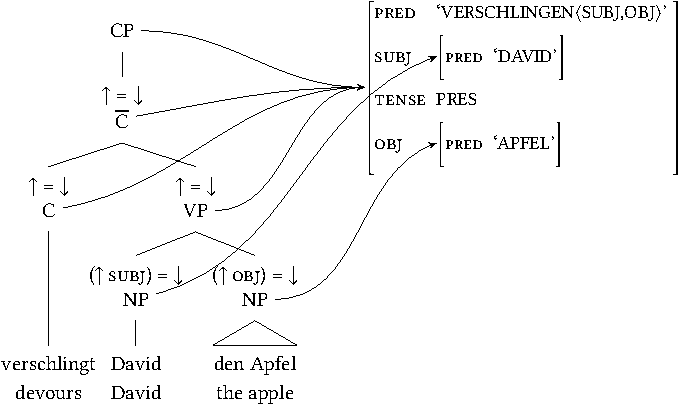
\includegraphics[width=.9\textwidth]{Figures/verschlingt-david-den-apfel-lfg-lsp-crop}

\bigskip

Analyse frei nach \citet[\page 41]{Berman2003a}.


}


\subsection{Lokale Umstellungen}

\frame{
\frametitle{Lokale Umstellungen}

\begin{itemize}
\item Zwei Möglichkeiten werden in der Literatur diskutiert:
      \begin{itemize}
      \item Umstellung von Argumenten aus einer Basiskonfiguration wie in GB\\
            (siehe \citew{Choi99a-u})
\pause
      \item direkte Ableitung über Phrasenstrukturregeln (siehe \citew{Berman96a-u,Berman2003a})
      \end{itemize}
\end{itemize}

}

\frame[shrink=15]{
\frametitle{Unterspezifikation des Kasus in der c-Struktur}

\begin{itemize}
\item Die Regel, die wir schon kennen, sagt nichts über den Kasus oder die grammatischen Funktionen
  der Elemente aus:
\ea
VP $\to$ (NP) (NP) (NP) (V)
\z
Wenn man die grammatische Funktion einer NP erst in Abhängigkeit von ihrem Kasus bestimmt, dann kann
  man mit der Regel in (\mex{0}) alle Anordnungen der Nominalphrasen ableiten.

\item \citet[\page 37]{Berman2003a} schlägt ähnliche Analyse vor:\\
\ea
      (\down {\sc case}) = ACC $\Rightarrow$ (\up \lfgobj)=\down{}
\z

%% Nee, denn das macht sie mit Spur.
%%
%%       Problem bei Fernabhängigkeiten, da Vorfeldelemente nicht unbedingt zur obersten f-Struktur
%%       beitragen.
%% \ea
%% Wen glaubst du, dass ich getroffen habe.
%% \z
%% Wenn hier \emph{wen} (\up \lfgobj)=\down{} ist, wird die f-Struktur für \emph{glauben} inkohärent.

%\item Brutale Lösung: Aufzählung aller Permutationen mit Kasus und f-Struktur-Annotation in den
%Phrasenstrukturregeln.
%
% Wen glaubst du, dass Peter seinen Freund belehrt, dass ich getroffen habe.
% Wenn man statt \up obj einen Regulären Ausdruck (\up COMP* \lfgobj) verwenden würde,
% Dann könnte wen zu belehren gehen und ihn zu getroffen
%
% Peter hat ihm versprochen, öfter zu helfen.
%
\end{itemize} 


}



\subsection{Fernabhängigkeiten und Funktionale Ungewißheit}

\subsubsection{Diskursfunktionen}


\frame{
\frametitle{Fernabhängigkeiten: Diskursfunktionen (I)}


\begin{itemize}
\item Beobachtung: die versetzte Konstituente (\emph{Chris} in
(\mex{1})) ist durch zwei Funktionen ausgezeichnet:
\ea
Chris, we think that David saw.
\z

  \begin{itemize}
  \item eine \blaubf{Argumentfunktion}, die kanonisch an anderer
  Stelle realisiert w\"urde\\
  (im Beispiel \textsc{obj} des Verbs \emph{saw}),
\pause
  \item eine besondere Hervorhebung des informationsstrukturellen
  Status in diesem Satzgef\"uge -- eine sog.\ \blaubf{Diskursfunktion}\\
  (im Beispiel \textsc{topic} des Matrixsatzes).
  \end{itemize}
\end{itemize}

}

\frame{
\frametitle{Diskursfunktionen (II)}

\begin{itemize}
\item Grammatikalisierte Diskursfunktionen: \textsc{topic} und \textsc{focus}\\
      (daneben wird \textsc{subj} als Default"=Diskursfunktion klassifiziert).
  \begin{itemize}
  \item Nur \textbf{grammatikalisierte} Diskursfunktionen werden auf
  f-Struktur markiert, also solche, die einem festen syntaktischen
  Mechanismus unterliegen und mit dem Rest der Syntax interagieren.

%%   (F\"ur die umfassende Repr\"asentation von informationsstrukturellen
%%   Eigenschaften wird in LFG eine separate Informationsstruktur
%%   angenommen.)
\pause
  \item Im Gegensatz zu den Argumentfunktionen werden die
  Diskursfunktionen \textsc{topic} und \textsc{focus} nicht lexikalisch subkategorisiert\\
 (unterliegen also nicht der \emph{Completeness}- und
  \emph{Coherence}-Bedingung)
\pause
  \item \textsc{topic} und \textsc{focus} werden 
%\"uber funktionale oder anaphorische Kontrolle 
  mit einer f-Struktur identifiziert,\\
  die eine Argument-Funktion tr\"agt.
  \end{itemize}
\end{itemize}

}

\frame{
\frametitle{Diskursfunktionen in der f-Struktur}
\smallframe

\eal
\ex Chris, we think that David saw.
\ex 
\lfgms{ pred & `think\sliste{ \lfgsubj, \comp }' \\
        topic & \rnode{topic}{\lfgms{ pred & `Chris' \\
                                   }}\\[4mm]
        subj & \lfgms{ pred & `pro'\\
                     }\\
        comp & \lfgms{ pred & `see\sliste{ \lfgsubj, \lfgobj }\\
                       subj & \lfgms{ pred & `David' \\
                                    }\\
                       obj  & \rnode{obj}{}\\
                     }\\
      }
\nccurve[ncurv=2.2]{topic}{obj}
\zl

\bigskip
Der Strich sagt: Der Wert von {\sc topic} ist mit dem von \textsc{comp obj} identisch.

Als Beschränkung: (\up  \textsc{topic})=(\up \textsc{comp obj})
}

\frame{
\frametitle{Verschiedene Einbettungstiefen (I)}

\eal
\ex Chris, we saw.
\ex 
\lfgms{ pred & `see\sliste{ \lfgsubj, \lfgobj }' \\
        topic & \rnode{topic}{\lfgms{ pred & `Chris' \\
                                   }}\\[4mm]
        subj & \lfgms{ pred & `pro'\\
                     }\\
        obj  & \rnode{obj}{}\\
      }
%\nodecurve[r]{topic}[r]{obj}{15em}
\nccurve[nodesepA=1pt,ncurv=2.2]{topic}{obj}
\zl

\bigskip

Als Beschränkung: (\up  \textsc{topic})=(\up \textsc{obj})
}


\frame{
\frametitle{Verschiedene Einbettungstiefen (II)}
\smallframe

\eal
\ex Chris, we think Anna claims that David saw.
\ex 
\scalebox{0.85}{%
\lfgms{ pred & `think\sliste{ \lfgsubj, \comp }' \\
        topic & \rnode{topic}{\lfgms{ pred & `Chris' \\
                                   }}\\[4mm]
        subj & \lfgms{ pred & `pro'\\
                     }\\
        comp & \lfgms{ pred & `claim\sliste{ \lfgsubj, \comp }\\
                       subj & \lfgms{ pred & `Anna' \\
                                   }\\
                       comp & \lfgms{ pred & `see\sliste{ \lfgsubj, \lfgobj }\\
                                      subj & \lfgms{ pred & `David' \\
                                                   }\\
                                      obj  & \rnode{obj}{}\\
                                    }\\
                     }\\
      }
%\nodecurve[r]{topic}[r]{obj}{15em}%
\nccurve[ncurv=2.2]{topic}{obj}
}
\zl

Als Beschränkung: (\up  \textsc{topic})=(\up \textsc{comp comp obj})
}

\frame{
\frametitle{Funktionale Ungewißheit}

\begin{itemize}
\item Die Beschränkungen sind c-Struktur-Beschränkungen:
\begin{tabular}{@{}ccc@{~=~}lc@{}}
CP & $\rightarrow$ & \multicolumn{2}{l}{\hspaceThis{(\up \textsc{topic})}XP} & C$'$ \\
 & &  (\up \textsc{topic}) & \down & \up=\down \\
 & &  (\up \textsc{topic}) & (\up \textsc{comp obj})\\
\end{tabular}

\pause
\item Wir haben aber auch andere Einbettungestiefen:

(\up  \textsc{topic})=(\up \textsc{obj})\\
(\up  \textsc{topic})=(\up \textsc{comp obj})\\
(\up  \textsc{topic})=(\up \textsc{comp comp obj})\\
\ldots

\pause
\item Die Generalisierung über diese Gleichungen ist:

(\up  \textsc{topic})=(\up \textsc{comp* obj})
\medskip

Dabei steht der `*' für beliebig viele Vorkommen von \comp.

\end{itemize}

}

\frame{
\frametitle{Disjunktionen und Variablen für grammatische Funktionen}


\begin{itemize}[<+->]
\item Im Deutschen kann nicht nur ein {\sc topic} im Vorfeld stehen,\\
      sondern auch ein \focus.
\item Man kann in LFG-Gleichungen auch Disjunktionen verwenden:

(\up  \textsc{topic$|$focus})=(\up \textsc{comp* obj})

\item Für \textsc{topic$|$focus} kann man einen eigenen Bezeichner einführen:\\
      {\sc df} steht für eine Disjunktion der Diskursfunktionen.


%% \begin{tabular}{@{}ccc@{~=~}lc@{}}
%% CP & $\rightarrow$ & \multicolumn{2}{l}{\hspaceThis{(\up \textsc{topic})}XP} & C$'$ \\
%%  & &  (\up \textsc{DF}) & \down & \up=\down \\
%%  & &  (\up \textsc{DF}) & (\up \textsc{comp* GF})\\
%% \end{tabular}

\end{itemize}

}

\subsection{Zusammenfassung}

\frame{
\frametitle{Zusammenfassung}

\begin{itemize}
\item LFG ist unifikationsbasiert, arbeitet mit Merkmalsstrukturen und PSG-Regeln
\item Grammatische Funktionen sind Primitive der LFG,\\
      sie sind nicht strukturell definiert (wie in der GB)
\item LFG ist lexikalistisch. Valenzänderungen wie bei Passivierung erfolgen im Lexikon
mittels lexikalischer Regeln.
\end{itemize}

}

% \subsection{Lexical Mapping Theory (LMT)}

\outline{

\begin{itemize}
\item Begriffe
\item Phrasenstrukturgrammatiken
\item Generalisierte Phrasenstrukturgrammatik (GPSG)
\item Lexikalisch-Funktionale Grammatik (LFG)
\item Lexical Mapping Theory (LMT)
\item PATR
\item Kategorialgrammatik (CG)
\item Kopfgesteuerte Phrasenstrukturgrammatik (HPSG)
%\item Konstruktionsgrammatik (CxG)
\item Baumadjunktionsgrammatik (TAG)
\end{itemize}
}

\frame{

}
\section{Kategorialgrammatik (CG)}

\outline{

\begin{itemize}
\item Begriffe
\item Phrasenstrukturgrammatiken
\item Government \& Binding (GB)
\item Generalisierte Phrasenstrukturgrammatik (GPSG)
\item Lexikalisch-Funktionale Grammatik (LFG)
%\item Lexical Mapping Theory (LMT)
%\item PATR
\item \blaubf{Kategorialgrammatik (CG)}
\item Kopfgesteuerte Phrasenstrukturgrammatik (HPSG)
\item Konstruktionsgrammatik (CxG)
\item Baumadjunktionsgrammatik (TAG)
\end{itemize}
}



\frame{
\frametitle{Kategorialgrammatik}

\begin{itemize}
\item Kategorialgrammatik ist die älteste der hier besprochenen Theorien \citep{Ajdukiewicz35a-u}.
\item Heute hauptsächlich in Edinburgh, Uetrecht und Amsterdam betrieben.
\item Wichtige Artikel und Bücher von \citet{Steedman91a,Steedman2000a-u,SB2006a-u}
\end{itemize}

}

\subsection{Allgemeines zum Repräsentationsformat}


\frame{
\frametitle{Motivation der Kategorialgrammatik}


\begin{itemize}
\item komplexe Kategorien ersetzen das \subcat"=Merkmal der GPSG

\medskip
\begin{tabular}[t]{@{}l@{\hspace{1cm}}l}
Regel                              & Kategorie~im~Lexikon\\
vp $\to$ v(ditrans) np~np          & (vp/np)/np  \\
vp $\to$ v(np\_and\_pp) np~pp(to)  & (vp/pp)/np  \\
\end{tabular}
\medskip


%
\pause
\item Es gibt nur noch sehr wenige, sehr abstrakte Regeln:

\ea
\blaubf{Multiplikationsregel}\\
\emph{Regel1}: X/Y * Y = X 
\z

Diese Regel sagt: Kombiniere ein X, das ein Y sucht, mit dem Y,\\
wenn es rechts von X/Y steht.
\pause

\item Valenz ist nur noch einmal kodiert, nämlich im Lexikon.

Bisher Valenz in den Grammatikregeln und im \subcat-Merkmal des Lexikoneintrags.
\end{itemize}
}

\frame{
\frametitle{Ein Beispiel}


\ea
\blaubf{Multiplikationsregel}\\
\emph{Regel1}: X/Y * Y = X 
\z

Diese Regel sagt: Kombiniere ein X, das ein Y sucht, mit dem Y,\\
wenn es rechts von X/Y steht.

%% \begin{center}
%%   \deriv{3}{
%%      \ccggf{I}  & \ccggf{saw} & \ccggf{the~man} \\
%%      \uline{1}  & \uline{1} & \uline{1}\\
%%      \ccgcf{NP} & \ccgcf{(S\bs NP)/NP} & \ccgcf{NP}\\
%%       &  \fapply{2}  \\
%%        & \gccmc{2}{\ccgcf{S\bs NP}} \\
%%        \bapply{3}  \\
%%       \cgmc{3}{\ccgcf{S}}
%%      }
%% \end{center}

\deriv{2}{
%\begin{tabular}{@{}cc@{}}
chased       & Mary\\
%\uline{1}    & \uline{1} \\
\hr & \hr\\
vp/np   & np\\
\multicolumn{2}{@{}c@{}}{\visible<2->{\forwardapp}} \\
\multicolumn{2}{@{}c@{}}{\visible<2->{vp}}\\
%\cgmc<2->{2}{vp}\\
%\end{tabular}
}


\pause
%\item für `/' meist Linksassoziativität \dh (vp/pp)/np = vp/pp/np

\pause

Kategorie v wird nicht mehr benötigt.

}

\frame{
\frametitle{Kategorialgrammatik}

\begin{itemize}
\item vp kann auch eleminiert werden: vp = s$\backslash$np

\ea
\emph{Regel2}: Y * X$\backslash$Y = X 
\z

\pause
\deriv{4}{
the  & cat & chased         & Mary\\
\hr  & \hr & \hr            & \hr\\
np/n & n   & (s\bs np)/np   & np\\
\multicolumn{2}{@{}c}{\visible<3->{\forwardapp}} & \multicolumn{2}{c@{}}{\visible<4->{\forwardapp}}\\
\multicolumn{2}{c}{\visible<3->{np}}             & \multicolumn{2}{c@{}}{\visible<4->{s\bs np}}\\
\multicolumn{4}{@{}c@{}}{\visible<5->{\backwardapp}}\\
\multicolumn{4}{c@{}}{\visible<5->{s}}\\
}

\pause\pause\pause
\pause
\item kein expliziter Unterschied zwischen Phrasen und Wörtern:
\begin{itemize}
\item intransitives Verb = Verbphrase = $(s \backslash np)$
\item genauso Eigennamen = Nominalphrasen = np
\end{itemize}
\end{itemize}
}


\frame{

\frametitle{Modifikation}

\begin{itemize}
\item optionale Modifikatoren:

vp $\to$ vp~pp \\
noun $\to$ noun~pp

beliebig viele PPen nach einer VP bzw.\ einem Nomen
\pause
\item Modifikatoren allgemein haben Form: $X \backslash X$ bzw.\ $X / X$
\pause
\item Prämodifikator für Nomina:

noun $\to$ adj~noun\\

Adjektive = $n/n$
\pause
\item Postmodifier für Nomina: $n \backslash n$
\pause
\item vp-Modifikator $\to$  X = $s \backslash np$
\pause
\item vp-Modifikator: $(s \backslash np) \backslash (s \backslash np)$. 

\end{itemize}
}

\frame{
\frametitle{Ableitung mit einer Kategorialgrammatik}
\vfill
% Eine typische Kategorialgrammatik benutzt nur s, np und n als Hauptkategorien. Manchmal werden noch pps als
% Komplementpräpositionalphrasen zugelassen.

% Eine Ableitung in der CG ist im wesentlichen ein binär verzweigender Baum, wird aber meistens wie folgt repräsentiert:
% Ein Pfeil unter einem Paar von Kategorien zeigt an, daß diese mit einer Kombinationsregel kombiniert werden.
% Die Richtung des Pfeils gibt die Richtung der Kombination an. Das Ergebnis wird unter den Pfeil geschrieben.
% Ein Beispiel zeigt Abbildung \ref{abb-cg}.

\oneline{%
\deriv{9}{
The  & small & cat & chased       & Mary & quickly                & round                     & the & garden\\
\hr  & \hr   & \hr & \hr          & \hr  & \hr                    & \hr                       & \hr & \hr\\
np/n & n/n   & n   & (s\bs np)/np & np   & (s\bs np)\bs (s\bs np) & (s\bs np)\bs (s\bs np)/np & np/n & n\\
     & \multicolumn{2}{c}{\forwardapp} & \multicolumn{2}{c@{}}{\forwardapp}\\
     & \multicolumn{2}{c}{n}           & \multicolumn{2}{c@{}}{s\bs np}\\
\multicolumn{3}{@{}c}{\forwardapp}        & \multicolumn{3}{c@{}}{\backwardapp}\\
\multicolumn{3}{@{}c}{np}                 & \multicolumn{3}{c@{}}{s\bs np}\\
&&&&&&&\multicolumn{2}{c@{}}{\forwardapp}\\
&&&&&&&\multicolumn{2}{c@{}}{np}\\
&&&&&&\multicolumn{3}{c@{}}{\forwardapp}\\
&&&&&&\multicolumn{3}{c@{}}{(s\bs np)\bs (s\bs np)}\\
&&&\multicolumn{6}{c@{}}{\backwardapp}\\
&&&\multicolumn{6}{c@{}}{s\bs np}\\
\multicolumn{9}{@{}c@{}}{\backwardapp}\\
\multicolumn{9}{@{}c@{}}{s}\\
}}
% Eine Kategorialgrammatik mit den beiden Multiplikationsregeln, die oben angegeben wurden, ist schwach äquivalent
% zu einer kontextfreien Grammatik. Solche Grammatiken wurden zuerst von Ajdukiewicz diskutiert. Die Äquivalenz
% zu den CFG wurde von Bar-Hillel bewiesen. Deshalb wird ein solches System auch AB genannt. 

% Obwohl AB schwach äquivalent zu kontextfreien Grammatiken ist, ermöglicht das System die Beschreibung
% verschiedener linguistischer Phänomene auf elegante Weise. In der CFG müßte man für entsprechende
% Beschreibungen Merkmale benutzen.
\vfill
}


\subsection{Verbstellung}

\subsubsection{Variable Verzweigung}

\frame{
\frametitle{Verbstellung}

\begin{itemize}
\item \citet[S.\,159]{Steedman2000a-u} für das Niederländische:

\eal
\ex gaf (`geben') mit Verbletztstellung: (S\sub{+SUB}$\backslash$NP)$\backslash$NP
\ex gaf (`geben') mit Verberststellung: (S\sub{$-$SUB}/NP)/NP
\zl

Das eine \emph{geben} verlangt Argumente rechts und das andere links von sich.

\pause
\item Die beiden Lexikoneinträge werden über Lexikonregeln zueinander in Beziehung gesetzt.

\end{itemize}


}
\frame{
\frametitle{Anmerkung zu dieser Analyse der Verbstellung}

Man beachte: Die NPen müssen in verschiedenen Reihenfolgen mit dem Verb kombiniert werden. Die
  Normalstellung entspricht:

\eal
\ex mit Verbletztstellung: (S\sub{+SUB}$\backslash$NP[nom])$\backslash$NP[acc]
\ex mit Verberststellung: (S\sub{$-$SUB}/NP[acc])/NP[nom]
\zl

Zur Kritik an solchen Analysen mit variabler Verzweigung siehe \citew{Mueller2005c}.


}


\subsubsection{Verbstellung mit Spur}

\frame{
\frametitle{Verbstellung mit Spur}

\citet{Jacobs91a} schlägt eine Spur in Verbletztstellung vor,\\
die die Argumente des Verbs und das Verb in Erststellung selbst als Argument verlangt.


}


\subsection{Konstituentenstellung}

\frame{
\frametitle{Konstituentenstellung}


\begin{itemize}
\item Bisher haben wir Kombination nach links und Kombination nach rechts gesehen.
      Die Abbindung der Argumente erfolgte immer in einer festen Reihenfolge (von außen nach
      innen).

\pause
\item \citet{SB2006a-u} unterscheiden: 
      \begin{itemize}
      \item Sprachen, in denen die Reihenfolge der Abbindung egal ist
\pause
      \item Sprachen, in denen die Richtung der Kombination egal ist
      \end{itemize}

\pause
\vfill
\begin{tabular}{@{}lll@{}}
Englisch   & (S$\backslash$NP)/NP     & S(VO)\\
Latein     & S\{$|$NP[nom], $|$NP[acc] \} & freie Stellung\\
Tagalog    & S\{/NP[nom], /NP[acc] \} & freie Stellung, verbinitial\\
Japanisch  & S\{$\backslash$NP[nom], $\backslash$NP[acc] \} & freie Stellung, verbfinal\\
\end{tabular}

\vfill
Elemente in Klammern in beliebiger Reihenfolge abbindbar

Steht `$|$' statt `$\backslash$' oder `/', dann ist die Abbindungsrichtung egal.

\end{itemize}

}

\subsection{Passiv}

\frame{
\frametitle{Passiv}

Lexikonregel:
\eal
\ex lieben: S\sub{+SUB} \{ $\backslash$NP[nom]$_i$, $\backslash$NP[acc]$_j$ \}
\ex geliebt: S\sub{pas} \{ $\backslash$NP[nom]$_j$, $\backslash$PP[von]$_i$ \}
\zl

}


\subsection{Fernabhängigkeiten}


\frame{
\frametitle{Fernabhängigkeiten}

\citet[S.\,614]{SB2006a-u}:
\ea
the man that Manny says Anna married
\z
\pause

Lexikoneintrag für Relativpronomen:
\ea
(N$\backslash$N)/(S/NP)
\z
Wenn ich rechts von mir einen Satz finde, dem noch eine NP fehlt,\\
dann kann ich mit dem zusammen einen N-Modifikator (N$\backslash$N) bilden. 

Das Relativpronomen ist in dieser Analyse der Kopf (Funktor).



}


\subsubsection{Type Raising}

\frame{
\frametitle{Type Raising}



Die Kategorie np kann durch {\em type raising} in die Kategorie $(s/(s\backslash np))$
umgewandelt werden. Kombiniert man diese Kategorie mit $(s\backslash np)$ erhält man dasselbe Ergebnis
wie bei einer Kombination von np und $(s\backslash np)$ mit Regel 2.
\eal
\ex np * s $\backslash$ np $\to$ s 
\ex s / (s $\backslash$ np) * s $\backslash$ np $\to$ s
\zl

\pause

Man dreht durch Type Raising die Selektionsrichtung um.

In (\mex{0}a) selegiert ein Verb (bzw.\,s) links von sich eine NP,\\
in (\mex{0}b) selegiert ein Nomen rechts von sich ein Verb (s),\\
das links von sich eine NP erwartet.

Das Ergebnis der Kombination ist in beiden Fällen ein Satz.




}


\subsubsection{Vorwärts- und Rückwärtskomposition}

\frame{
\frametitle{Vorwärts- und Rückwärtskomposition}

\ea
\begin{tabular}[t]{@{}l@{\hspace{1cm}}l}
X/Y * Y/Z = X/Z & Vorwärtskomposition~(fc) \\
Y$\backslash$Z * X$\backslash$Y = X$\backslash$Z & Rückwärtskomposition~(bc)
\end{tabular}
\z 

Beispiel Vorwärtskomposition:

Wenn ich Y finde, bin ich ein vollständiges X.

Ich habe ein Y, dem aber noch ein Z fehlt.

Wenn ich dieses Element mit X/Y verbinde, bekomme ich etwas,\\
das ein X ist, wenn es noch mit einem Z verbunden wird.

%% \begin{tabular}{@{}llll@{}}
%% Fido                & chased  & Mary\\
%% S/(S$\backslash$NP) & (s$\backslash$np)/np   & np\\
%% \multicolumn{2}{c}{\visible<3->{np}}        & \multicolumn{2}{c}{\visible<4->{s$\backslash$np}}\\
%% \multicolumn{4}{c}{\visible<5->{s}}\\
%% \end{tabular}

%% \pause\pause\pause
%% \pause
}


\subsubsection{Relativsätze mit Fernabhängigkeiten}


\frame{
\frametitle{Relativsätze mit Fernabhängigkeiten}


\deriv{5}{
that                                & Manny                                                   & says                              & Anna                 & married\\
\hr                                 & \forwardt                                               & \hr                               & \forwardt            & \hr \\
%
%
(N\bs N)/\braun<5->{(S/NP)} & S/\rot<2->{(S\bs NP)}                           & \rot<2->{(S\bs NP)}/S     & S/\gruen<3->{(S\bs NP)} & \gruen<3->{(S\bs NP)}/NP\\
                                    & \multicolumn{2}{c}{\visible<2->{\forwardc}} & \multicolumn{2}{c@{}}{\visible<3->{\forwardc}}\\
%
%
                                    & \multicolumn{2}{c@{}}{\visible<2->{S/\blau<4->{S}}}                    & \multicolumn{2}{c@{}}{\visible<3->{\blau<4->{S}/NP}}\\
                                    & \multicolumn{4}{c@{}}{\visible<4->{\forwardc}}\\
                                    & \multicolumn{4}{c@{}}{\visible<4->{\braun<5->{S/NP}}}\\
\multicolumn{5}{@{}c@{}}{\visible<5->{\forwardapp}}\\
\multicolumn{5}{@{}c@{}}{\visible<5->{N\bs N}}\\
}



}


\frame{
\frametitle{Anmerkung zu dieser Relativsatzanalyse}


Die Annahme, dass das Relativpronomen der Kopf ist, ist problematisch, da Rattenfängerkonstruktionen
wie (\mex{1}) nicht einfach erklärt werden können \citep{Pollard88a}.


\eal
\ex Here's the minister [[in [the middle [of [whose sermon]]]] the dog barked].\footnote{
\citet[S.\,212]{ps2}
}
\ex Reports [the height of the lettering on the covers of which] the government prescribes should be
abolished.\footnote{
\citet[S.\,109]{Ross67}\nocite{Ross86a-u}
}
\zl

Zu Analysen siehe \citep{Morrill95a,Steedman97a}.

}

\subsection{Übungsaufgabe}

\frame{
\frametitle{Übungsaufgabe}


Analysieren Sie den Satz:
\ea
Die Kinder im Zimmer lachen laut.
\z





}

%\section{PATR-II}

\outline{

\begin{itemize}
\item Begriffe
\item Phrasenstrukturgrammatiken
\item Generalisierte Phrasenstrukturgrammatik (GPSG)
\item Lexikalisch-Funktionale Grammatik (LFG)
\item Lexical Mapping Theory (LMT)
\item PATR
\item Kategorialgrammatik (CG)
\item Kopfgesteuerte Phrasenstrukturgrammatik (HPSG)
%\item Konstruktionsgrammatik (CxG)
\item Baumadjunktionsgrammatik (TAG)
\end{itemize}
}

\frame{

}
\section{HPSG}

\outline{

\begin{itemize}
\item Begriffe
\item Phrasenstrukturgrammatiken
\item Government \& Binding (GB)
\item Generalisierte Phrasenstrukturgrammatik (GPSG)
\item Lexikalisch-Funktionale Grammatik (LFG)
%\item Lexical Mapping Theory (LMT)
%\item PATR
\item Kategorialgrammatik (CG)
\item \blau{Kopfgesteuerte Phrasenstrukturgrammatik (HPSG)}
\item Konstruktionsgrammatik (CxG)
\item Baumadjunktionsgrammatik (TAG)
\end{itemize}
}


\frame{
\frametitle{Head-Driven Phrase Structure Grammar (HPSG)}


\begin{itemize}[<+->]
\item Von Carl Pollard und Ivan Sag Mitte der 80er Jahre entwickelt\\
      \citep{ps,ps2}
\item HPSG gehört wie LFG zur West-Coast-Linguistik.
\item Lehrmaterial und Überblicksartikel:\\
      \citew{MuellerLehrbuch3,MuellerArten,LM2006a,MuellerCurrentApproaches}\nocite{Mueller99a,Mueller2002b}
\item Handbuch mit Einführung und Überblickskapiteln zu diversen Phänomenen und Theorievergleich: \citet*{HPSGHandbook}
\item Ivan Sag war einer derjenigen, die GPSG entwickelt haben.
\end{itemize}




}


\subsection{Allgemeines zum Repräsentationsformat}

\frame{

\frametitle{Grundlegendes zur HPSG}
\small
\begin{itemize}
\item lexikalisiert (head-driven/kopfgesteuert)
\pause
\item zeichenbasiert \citep{Saussure16a-de}
\pause
%\item unifikationsbasiert
\item getypte Merkmalstrukturen (Lexikoneinträge, Phrasen, Prinzipien)
\pause
\item Mehrfachvererbung
\pause
\item monostratale Theorie\\~\\
\begin{minipage}[t]{2.5cm}
~\\[-20mm]
\begin{itemize}
\item \blau<6>{Phonologie}\rnode{1}{}
\item \blau<7>{Syntax}\rnode{2}{}
\item \blau<8>{Semantik}\rnode{3}{}
\end{itemize}
\end{minipage}%
\parbox[t]{3cm}{
\resizebox{5cm}{!}{
\(
\ms[word]{
\rnode{4}{phon}   & \blau<6>{\phonliste{ Grammatik }} \\[1mm]
synsem$|$loc & \ms[loc]{ \rnode{5}{cat}  & \blau<7>{\ms[cat]{ head & \ms[noun]{ case & \ibox{1}\\
                                                       }\\[6mm]
                                       spr & \liste{ DET[{\sc case}~\ibox{1}] } \\
                                     }} \\[6mm]
              \rnode{6}{cont} & \blau<8>{\ldots \ms[grammatik]{ inst & X \\
                                   }}\\
            }\\
}
\)
}
}
\end{itemize}
}

\frame{
\frametitle{Einflüsse}

\begin{itemize}[<+->]
\item Kategorialgramamtik\\
      (Funktor-Argument-Strukturen, Valenz, Argumentkomposition)
\item GPSG\\
      (ID/LP-Format, Slash-Mechanismus für Fernabhängigkeiten)
\item Government \& Binding\\
      (u.a.\,Analyse der Verbstellung im Deutschen)
\end{itemize}



}


\frame{
\frametitle{Valenz und Grammatikregeln: PSG}


\begin{itemize}
\item große Anzahl von Regeln:\\
      \begin{tabular}[t]{l@{~$\to$~}l@{\hspace{6em}}l}
      S &  NP, V               & {\em X schläft\/}\\
      S &  NP, NP, V           & {\em X Y liebt\/}\\
      S &  NP, PP[{\it über\/}], V           & {\em X über Y spricht\/}\\
      S &  NP, NP, NP, V       & {\em X Y Z gibt\/}\\
      S &  NP, NP, PP[{\it mit\/}], V       & {\em X Y mit Z dient\/}\\
      \end{tabular}
\pause
\item Verben müssen mit passender Regel verwendet werden.
\end{itemize}

}

\frame{

\frametitle{Valenz und Grammatikregeln: HPSG}

\begin{itemize}
\item Argumente als komplexe Kategorien in der lexikalischen Repräsentation
      eines Kopfes repräsentiert\\
      (wie Kategorialgrammatik)
\pause
\item \begin{tabular}[t]{@{}lll}
      Verb             & \comps\\
      {\em schlafen\/} & \sliste{ NP }\\
      {\em lieben\/}   & \sliste{ NP, NP }\\
      {\em sprechen\/} & \sliste{ NP, PP[{\it über\/}] }\\
      {\em geben\/}    & \sliste{ NP, NP, NP }\\
      {\em dienen\/}   & \sliste{ NP, NP, PP[{\it mit\/}] }\\  
      \end{tabular}
\end{itemize}


}

\frame{
\frametitle{Beispielstruktur mit Valenzinformation (I)}

\vfill
\hfill
\begin{forest}
sm edges
[V{[\comps \eliste]}
	[{\ibox{1} NP[\type{nom}]}
		[Peter]]
	[V{[\comps \sliste{ \ibox{1} }]}
		[schläft]]]
\end{forest}
\hfill\hfill\mbox{}
\vfill
V[\comps \sliste{ }] entspricht hierbei einer vollständigen Phrase\\
(VP oder auch S)
\vfill
}

\frame{
\frametitle{Beispielstruktur mit Valenzinformation (II)}

\vfill
\hfill
\begin{forest}
sm edges
[V{[\comps \eliste]}
	[{\ibox{1} NP[\type{nom}]}
		[Peter]]
	[V{[\comps \sliste{ \ibox{1} }]}
		[{\ibox{2} NP[\type{acc}]}
			[Maria]]
		[V{[\comps \sliste{ \iboxsp{1}, \ibox{2} }]}
			[erwartet]]]]
\end{forest}\hfill\hfill\mbox{}
\vfill

}



\frame{
\frametitle{SOV vs.\ SVO: Repräsentation von Subjekten}

\begin{itemize}
\item Wissenschaftler*innen, die zum Deutschen arbeiten, nehmen an, dass das Subjekt finiter Verben
  sich wie andere Argumente verhält. (\citealp{Pollard90a-Eng}; \citealp[\page 376]{Eisenberg94b})

HPSG: Subjekte und Komplemente werden auf derselben Valenzliste repräsentiert (\comps).

\pause
\item English: Subjekte sind anders.
\pause
\item \argst ist die zugrundeliegende Repräsentation, die alle Argumente enthält. \citep{DKW2021a}
\pause
\item Sprachabhängige Verteilung auf die Valenzmerkmale \spr und \comps.

\medskip
\oneline{%
\begin{tabular}[t]{@{}llll}
      verb          & \spr                      & \comps                                     & \argst\\
      \emph{sleep}  & \sliste{ NP[\type{nom}] } & \sliste{}                                  & \sliste{ NP[\type{nom}] }\\
      \emph{expect} & \sliste{ NP[\type{nom}] } & \sliste{ NP[\type{acc}] }                  & \sliste{ NP[\type{nom}], NP[\type{acc}] }\\
      \emph{speak}  & \sliste{ NP[\type{nom}] } & \sliste{ PP[\type{about}] }                & \sliste{ NP[\type{nom}], PP[\type{about}] }\\
      \emph{give}   & \sliste{ NP[\type{nom}] } & \sliste{ NP[\type{acc}], NP[\type{acc}] }  & \sliste{ NP[\type{nom}], NP[\type{acc}], NP[\type{acc}] }\\
      \emph{serve}  & \sliste{ NP[\type{nom}] } & \sliste{ NP[\type{acc}], PP[\type{with}] } & \sliste{ NP[\type{nom}], NP[\type{acc}], PP[\type{with}] }\\  
      \end{tabular}}

\end{itemize}


}

\frame{
\frametitle{Beispielanalyse mit \spr und \comps}

\centerline{%
\scalebox{.8}{%
\begin{forest}
sm edges
[V{\feattab{\spr \eliste,\\
            \comps \eliste}}
  [\ibox{1} NP [Kim]]
  [V{\feattab{\spr \sliste{ \ibox{1} },\\
              \comps \eliste}}
    [V{\feattab{\spr \sliste{ \ibox{1} },\\
                \comps \sliste{ \ibox{2} }}}
      [talks]]
    [\ibox{2} P{\feattab{\spr \sliste{ },\\
                \comps \sliste{ }}}
      [P{\feattab{\spr \sliste{ },\\
                \comps \sliste{ \ibox{3} }}} [about]]
      [\ibox{3} N{\feattab{\spr \sliste{ },\\
                     \comps \sliste{ }}}
        [\ibox{4} Det [the]]
        [N{\feattab{\spr \sliste{ \ibox{4} },\\
                     \comps \sliste{ }}} [summer] ]]]]]
\end{forest}}}

}


\subsubsection{Repräsentation der Konstituentenstruktur}

\frame{
\frametitle{Repräsentation der Konstituentenstruktur}

\centerline{%
\begin{forest}
sm edges
[NP
	[Det
		[dem;the]]
	[N
		[Mann;man]]]
\end{forest}
}

Der Baum kann mit Merkmalsbeschreibungen repräsentiert werden:

\ea
\ms{ 
  phon     & \phonliste{ dem Mann }\\[1mm]
  head-dtr & \onems{ phon \phonliste{ Mann }
                 }\\
  non-head-dtrs & \sliste{ \onems{ phon \phonliste{ dem }
                            }}
}
\z

}

\subsubsection{Feature geometry}

\frame{
\frametitle{Komplette Merkmalsgeometrie}

\ea
\label{LE-Grammatik}
\scalebox{.7}{%
\ms[word]{
phon   & \phonliste{ Grammatik } \\[1mm]
synsem & \ms{ loc & \ms[local]{ cat  & \ms[category]{ head & \ms[noun]{ case & \ibox{1}
                                                                      }\\[3mm]
                                                     spr & \sliste{ Det[\textsc{case}~\ibox{1}] }\\
                                                     comps & \eliste\\[1pt]
                                                    } \\[6mm]
                                cont & \ms[mrs]{
                                       ind & \ibox{2} \ms{ per & third\\
                                                           num & sg\\
                                                           gen & fem\\
                                                         }\\
                                       rels & \sliste{ \ms[grammatik]{ inst & \ibox{2} 
                                                                    } }
                                        }
                              }\\
               nonloc & \ms{ inher$|$slash   & \eliste{}\\
                             to-bind$|$slash & \eliste{}\\
                           }
            }
}}
\z

Information, die für Strukturteilung gebraucht wird, wird zusammen gruppiert.


}

\subsubsection{ID-Schemata}

\frame{
\frametitle{Das Kopf-Komplement-Schema (vorläufig)}


\type{head-complement-phrase}\istype{head"=complement"=phrase} \impl\\
\onems{
      synsem$|$loc$|$cat$|$comps \ibox{1} \\
      head-dtr$|$synsem$|$loc$|$cat$|$comps \ibox{1} $\oplus$ \sliste{ \ibox{2} } \\
      non-head-dtrs \sliste{ [ \synsem \ibox{2} ] }
      }

\pause

\ea
\onems[head-complement-phrase]{
phon \phonliste{ Peter schläft }\\
synsem$|$loc$|$cat$|$comps \eliste\\
head-dtr \onems{ phon \phonliste{ schläft }\\
                 synsem$|$loc$|$cat$|$comps \sliste{ \ibox{1} NP[\type{nom}] }
               }\\
non-head-dtrs \sliste{ \onems{ phon \phonliste{ Peter }\\
                               \synsem \ibox{1}
                             } }
}
\z


}

\subsubsection{LP-Regeln}

\frame{
\frametitle{Linearisierungsregeln}

\eal
\ex\label{lp-ini-arg} 
Head[\initial$+$] $<$ Complement
\ex 
Complement $<$ Head[\initial --]
\zl

\pause
Präpositionen haben \initialw `$+$' und müssen deshalb ihren Argumenten vorangehen.
\eal
\ex[]{
{}[in [den Schrank]]
}
\ex[*]{
{}[[den Schrank] in]
}
\zl
\pause
Verben in Letztstellung haben den Wert `$-$' und müssen ihren Argumenten folgen.
\eal
\ex[]{
{}dass [er [ihn umfüllt]]
}
\ex[*]{
{}dass [er [umfüllt ihn]]
}
\zl


}


\subsubsection{Kopfmerkmale}

\frame{
\frametitle{Kopfmerkmale}

\begin{itemize}
\item Information über die Verbform muss am obersten Knoten der Projektion verfügbar sein:
\eal
\label{bsp-projektion-v-merkmale}
\ex[]{
{}[Dem Mann helfen] will er nicht.
}
\ex[]{
{}[Dem Mann geholfen] hat er nicht.
}
\ex[*]{
{}[Dem Mann geholfen] will er nicht.
}
\ex[*]{
{}[Dem Mann helfen] hat er nicht.
}
\zl
\end{itemize}
}


\frame{
\frametitle{Projektion von Merkmalen entlang des Kopfpfades}

\settowidth{\offset}{V[\type{fi}}
\settowidth{\offsetup}{V[\type{fin}}
\centerline{
\begin{forest}
sm edges, for tree={l+=\baselineskip}
[\gruen{V}{[\gruen{\type{fin}}, \comps \eliste]}, name=fin1
	[\ibox{1} NP{[\type{nom}]}
		[jemand]]
	[\gruen{V}{[\gruen{\type{fin}}, \comps \sliste{ \ibox{1} }]}, name=fin2
		[\ibox{2} NP{[\textit{dat}]}
			[dem Kind,roof]]
		[\gruen{V}{[\gruen{\type{fin}}, \comps \sliste{ \ibox{1}, \ibox{2} }]}, name=fin3
			[\ibox{3} NP{[\textit{acc}]}
				[das Buch,roof]]
			[\gruen{V}{[\gruen{\type{fin}}, \comps \sliste{ \ibox{1}, \ibox{2}, \ibox{3} }]}, name=fin4
				[gibt]]]]]	
tikz={\draw[<->] ($(fin1.south west)+(\offsetup,0)$) to ($(fin2.north west)+(\offset,0)$);
      \draw[<->] ($(fin2.south west)+(\offsetup,0)$) to ($(fin3.north west)+(\offset,0)$);
      \draw[<->] ($(fin3.south west)+(\offsetup,0)$) to ($(fin4.north west)+(\offset,0)$);}
\end{forest}
}

}

\frame{
\frametitle{Strukturteilung der \head-Werte}

\centerline{
\scalebox{.8}{%
\begin{forest}
sm edges
[\ms{head & \gruen{\ibox{1}}\\
     comps & \sliste{ }
     }
	[{\ibox{2} NP{[\type{nom}]}}
		[jemand]]
	[\ms{
             head & \gruen{\ibox{1}}\\
             comps & \sliste{ \ibox{2} }
             }
		[\ibox{3} NP{[\textit{dat}]}
			[dem Kind, roof]]
		[\ms{
                                                                                   head & \gruen{\ibox{1}}\\
                                                                                   comps & \sliste{ \ibox{2}, \ibox{3} }
                                                                                    }
			[\ibox{4} NP{[\textit{acc}]}
				[das Buch, roof]]
			[\ms{
                                                                                   head & \gruen{\ibox{1} \ms[verb]{
                                                                                                  vform & fin
                                                                                                  }}\\
                                                                                   comps & \sliste{ \ibox{2}, \ibox{3}, \ibox{4} }
                                                                                    }
				[gibt]]]]]	
\end{forest}}}
}


\subsubsection{Typhierarchien und Vererbung}


\frame{
\frametitle{Typhierarchien und Vererbung}


\centerline{%
\begin{forest}
type hierarchy
[sign
  [word]
  [phrase 
    [non-headed-phrase]
    [headed-phrase [head-complement-phrase]]]]
\end{forest}}

\begin{itemize}
\item Alle Merkmalstrukutren sind in der HPSG getypt.
\pause
\item Typen werden in Hierarchien geordnet.
\pause
\item Subtypen erben Beschränkungen von Obertypen.

\pause

\item Beispiel: \type{headed-phrase}
\ea
\type{headed"=phrase}\istype{headed"=phrase} \impl
\ms{ 
synsem$|$loc$|$cat$|$head \ibox{1}\\
head-dtr$|$synsem$|$loc$|$cat$|$head \ibox{1}\\
} 
\z


\end{itemize}


}


\frame{
\frametitle{Vererbung von Beschränkungen}

\begin{itemize}
\item
\ea
\label{head-arg-schema-hfp}
Head-Complement Schema + Head Feature Principle:\\
\onems[head-complement-phrase~]{
synsem$|$loc$|$cat  \ms{ \visible<2->{\gruen{head}   & \gruen{\ibox{1}}} \\
                          comps & \ibox{2}
                        }\\
head-dtr$|$synsem$|$loc$|$cat \ms{ \visible<2->{\gruen{head}   & \gruen{\ibox{1}}} \\
                                   comps & \ibox{2} $\oplus$ \sliste{ \ibox{3} }
                                 } \\
non-head-dtrs   \sliste{ [ synsem \ibox{3} ] }
}
\z
\medskip

Beschränkungen für \type{head-complement-phrase} \pause
und von \type{headed-phrase} geerbte Beschränkungen
\pause
\item Vererbungshierarchien sind wichtig, um Generalisierungen zu erfassen.\\
Sie werden im Bereich des Lexikons seit \citew*{FPW85a} benutzt.
\end{itemize}


}






\subsection{Passiv}

\frame{
\frametitle{Passiv}

\begin{itemize}[<+->]
\item HPSG folgt Bresnans Argumentation, dass das Passiv im Lexikon behandelt werden sollte.

\item Eine Lexikonregel nimmt den Verbstamm als Eingabe und lizenziert die Partizipform, wobei das
prominenteste Argument (das sogenannte designierte Argument) unterdrückt wird.

\item Da grammatische Funktionen in der HPSG keine Bestandteile der Theorie sind,
      braucht man auch keine Mapping-Prinzipien,\\
      die Objekte auf Subjekte mappen.

\item Allerdings muss die Kasusänderung bei Passivierung erklärt werden.
\end{itemize}



}

\subsubsection{Struktureller Kasus}

\frame{
\frametitle{Struktureller und lexikalischer Kasus}

\begin{itemize}
\item Wenn Kasus von Argumenten von der syntaktischen Umgebung abhängt,
      spricht man von \blau{strukturellem Kasus}. \\
      Ansonsten haben die Argumente \blau{lexikalischen Kasus}.
\pause
\item Beispiele für strukturellen Kasus sind:
\eal
\ex \blau{Der Installateur} kommt.
\pause
\ex Der Mann läßt \blau{den Installateur} kommen.
\pause
\ex das Kommen \blau{des Installateurs}
\zl

\pause
\item In (\mex{0}) handelt es sich um Subjektskasus, in (\mex{1}) um Objektskasus:
\eal
\ex Karl schlägt \blau{den Hund}.
\ex \blau{Der Hund} wird geschlagen.
\zl
\end{itemize}
}

\subsubsection{Lexikalischer Kasus}


\frame{
\frametitle{Lexikalische Kasus}

\begin{itemize}
\item Vom Verb abhängiger Genitiv ist lexikalischer Kasus:\\
      Bei Passivierung ändert sich der Kasus eines Genitivobjekts nicht.
\eal
\ex[]{
Wir gedenken \blau{der Opfer}.
}
\ex[]{
\blau{Der Opfer} wird gedacht.
}
\ex[*]{
\blau{Die Opfer} wird/werden gedacht.
}
\zl
\pause
(\mex{0}b) = unpersönliches Passiv, es gibt kein Subjekt.

\pause
\item Den Dativ zähle ich zu den lexikalischen Kasus (umstritten).
\pause
\item Zur Diskussion und weiteren Fällen von lexikalischem Kasus siehe \citew{MuellerLehrbuch3}.
\end{itemize}

}


\subsubsection{Valenzinformation und das Kasusprinzip}


\frame{
\frametitle{Valenzinformation und das Kasusprinzip}





\begin{prinzip-break}[\hypertarget{case-p}{Kasusprinzip (vereinfacht)}]
\label{case-p}
\begin{itemize}
\item In einer Liste, die sowohl das Subjekt als auch die Komplemente eines verbalen Kopfes
      enthält, bekommt das erste Element mit strukturellem Kasus 
      Nominativ.
\item Alle anderen Elemente der Liste, die strukturellen Kasus tragen, bekommen Akkusativ.
\end{itemize}
\end{prinzip-break}


}

\subsubsubsection{Aktiv}

\frame{
\frametitle{Aktiv}

prototypische Valenzlisten:
\ea
\begin{tabular}[t]{@{}l@{~}l@{~}l}
a. & \emph{schläft}:     & \comps \sliste{ NP[\type{str}]$_j$ }\\
b. & \emph{unterstützt}: & \comps \sliste{ NP[\type{str}]$_j$, NP[\type{str}]$_k$ }\\
c. & \emph{hilft}:       & \comps \sliste{ NP[\type{str}]$_j$, NP[\type{ldat}]$_k$ }\\
d. & \emph{schenkt}:     & \comps \sliste{ NP[\type{str}]$_j$, NP[\type{str}]$_k$, NP[\type{ldat}]$_l$ }\\
\end{tabular}
\z
\emph{str} steht für \emph{strukturell}, \emph{ldat} für lexikalischen Dativ.

\pause
Das erste Element in der \compsl bekommt Nominativ.\\
Alle anderen mit strukturellem Kasus bekommen Akkusativ.

}

\subsubsubsection{Kasusvergabe im Passiv}

\frame[shrink]{
\frametitle{Passiv}

\ea
\begin{tabular}[t]{@{}l@{~}l@{~}l}
a. & \emph{schläft}:     & \comps \sliste{ NP[\type{str}]$_j$ }\\
b. & \emph{unterstützt}: & \comps \sliste{ NP[\type{str}]$_j$, NP[\type{str}]$_k$ }\\
c. & \emph{hilft}:       & \comps \sliste{ NP[\type{str}]$_j$, NP[\type{ldat}]$_k$ }\\
d. & \emph{schenkt}:     & \comps \sliste{ NP[\type{str}]$_j$, NP[\type{str}]$_k$, NP[\type{ldat}]$_l$ }\\
\end{tabular}
\z

Bei Passivierung der Verben ergeben sich die folgenden \comps"=Listen:
\ea
\begin{tabular}[t]{@{}l@{~}l@{~}l}
a. & \emph{geschlafen wird}:  & \comps \sliste{ }\\
b. & \emph{unterstützt wird}: & \comps \sliste{ NP[\type{str}]$_k$ }\\
c. & \emph{geholfen wird}:    & \comps \sliste{ NP[\type{ldat}]$_k$ }\\
d. & \emph{geschenkt wird}:   & \comps \sliste{ NP[\type{str}]$_k$, NP[\type{ldat}]$_l$ }\\
\end{tabular}
\z
In (\mex{0}) steht jetzt eine andere NP an erster Stelle.\\
Wenn diese NP strukturellen Kasus hat, bekommt sie Nominativ,\\
wenn das wie in (\mex{0}c) nicht der Fall ist, bleibt der Kasus, wie er ist,\\
nämlich lexikalisch spezifiziert.
}

\subsection{Verbstellung}

\frame[shrink=5]{
\frametitle{\large Repräsentationen und Lexikonregeln: Verbbewegung}

~
\vfill
\hfill%
%\scalebox{0.85}{%
\begin{forest}
sm edges
[VP
	[V \sliste{ VP//V }, name=vini
	   [V,name=vlast [kennt$_j$]]]
	[VP//V, name=vp
	   [NP [jeder]]
	   [V$'$//V, name=vbar
	     [NP [diesen Roman, roof]]
		[V//V,name=vtrace [ \trace$_j$]]]]]
%\draw[<->] (vone) to (vtwo);
%%\draw (-2,-5) to[grid with coordinates] (4,0.5);
%% \draw[<-] (3,-3.4) .. controls (3.2,-3.6) .. (3.5,-3.4)
%%                    .. controls ()         .. (;
\draw[<->] ($(vtrace.south)+(-.25,.1)$)    to [bend right=45]  ($(vtrace.south)+(.25,.1)$);
\draw[<->] (vtrace)                        to [out=45, in=0]  (vbar);
\draw[<->] ($(vbar.north east)+(-0.2,0)$)  to [out=80, in=0]  (vp);
\draw[<->] ($(vp.north east)+(-0.25,-.1)$)  to [out=145,in=35] ($(vini.north east)+(-.5,-.1)$);
\draw[<->] ($(vini.south east)+(-.45,.1)$) to [bend left=30] ($(vlast.north east)+(-.1,-.1)$);
\end{forest}
%}
\hfill\hfill\mbox{}
\vfill

\begin{itemize}[<+->]
\item In Verberstsätzen steht in der Verbletztposition eine Spur.
\item In Verberststellung steht eine besondere Form des Verbs,\\
      die eine Projektion der Verbspur selegiert.
\item Dieser spezielle Lexikoneintrag ist durch eine Lexikonregel lizenziert.
\item Verbindung Verb/Spur durch Informationsweitergabe im Baum
\end{itemize}

}


\subsection{Lokale Umstellung}

\frame{
\frametitle{Lokale Umstellung}

Mehrere Möglichkeiten (zu Überblick siehe \citealt{MuellerOrder}):
\begin{itemize}
\item ganz flache Strukturen. Umordnung wie bei GPSG
\pause
\item binär verzweigende Strukturen,\\
      Abbindung der Argumente in beliebiger Reihenfolge
\pause
\item Lexikonregeln mit Umordnung der Elemente in Valenzlisten

\end{itemize}

}

\subsubsection{Binär verzweigende Strukturen}

\frame{
\frametitle{Beispiel: Normalabfolge}
\eal
\ex weil jeder diesen Roman kennt
\ex weil diesen Roman jeder kennt
\zl

\centerline{%
\begin{forest}
sm edges
[V{[\comps \sliste{}]}
	[\ibox{1} NP{[\type{nom}]}
		[jeder]]
	[V{[\comps \sliste{ \ibox{1} }]}
		[\ibox{2} NP{[\type{acc}]}
			[diesen Roman, roof]]
		[V{[\comps \sliste{ \iboxsp{1}, \ibox{2} }]}
			[kennt]]]]
\end{forest}
}%

}

\frame{
\frametitle{Beispiel: Umstellung}


\centerline{%
\begin{forest}
sm edges
[V{[\comps \sliste{}]}
	[\ibox{2} NP{[\type{acc}]}
		[diesen Roman, roof]]
	[V{[\comps \sliste{ \ibox{2} }]}
        	[\ibox{1} NP{[\type{nom}]}
	        	[jeder]]
		[V{[\comps \sliste{ \iboxsp{1}, \ibox{2} }]}
			[kennt]]]]
\end{forest}
}%

\medskip
Unterschied nur in Abbindungsreihenfolge der Elemente in \comps
}



\subsection{Fernabhängigkeiten}

\frame{

%\frametitle{Repräsentationen und Lexikonregeln: 
\frametitle{Konstituentenbewegung}

\vfill
\hfill%
\scalebox{0.7}{
\begin{forest}
sm edges
[VP
	[NP$_i$,name=np
		[diesen Roman,roof]]
	[VP/NP,name=vpnp2
		[V
			[V
				[kennt$_j$]]]
		[VP/NP,name=vpnp1
			[NP/NP, name=npnp
				[\trace$_i$]]
			[V$'$
				[NP
					[jeder]]
				[V
				  [\trace$_j$]]]]]]
\draw[<->] ($(npnp.east)$)  to [bend right=45] ($(vpnp1.south east)+(-.25,.1)$);
\draw[<->] ($(vpnp1.north east)+(-.26,-.1)$)  to [bend right=45] ($(vpnp2.east)+(-0,0)$);
\draw[<->] ($(vpnp2.north)+(.26,-0)$) parabola[parabola height=5mm] ($(np.north)+(-.15,0)$);
\end{forest}
}
\hfill\hfill\mbox{}
\vfill
\begin{itemize}[<+->]
\item Wie bei Verbbewegung: Spur an ursprünglicher "`normaler"' Position.
\item Weiterreichen der Information im Baum
\item Konstituentenbewegung ist nicht lokal, Verbbewegung ist lokal\\
      mit zwei verschiedenen Merkmalen modelliert ({\sc slash} vs.\ {\sc dsl})
\end{itemize}

}


\section{Konstruktionsgrammatik (CxG)}

\outline{

\begin{itemize}
\item Begriffe
\item Phrasenstrukturgrammatiken
\item Government \& Binding (GB)
\item Generalisierte Phrasenstrukturgrammatik (GPSG)
\item Lexikalisch-Funktionale Grammatik (LFG)
%\item Lexical Mapping Theory (LMT)
%\item PATR
\item Kategorialgrammatik (CG)
\item Kopfgesteuerte Phrasenstrukturgrammatik (HPSG)
\item \blaubf{Konstruktionsgrammatik (CxG)}
\item Baumadjunktionsgrammatik (TAG)
\end{itemize}
}

\frame{
\frametitle{Konstruktionsgrammatik (I)}

\begin{itemize}[<+->]
\item Konstruktionsgrammatik gehört auch zur West-Coast-Linguistik
\item Sie wurde maßgeblich von Charles Fillmore, Paul Kay und Adele Goldberg geprägt.
\citep*{FKoC88a,KF99a,Kay2002a,Kay2005a,Goldberg95a,Goldberg2006a}

\item Fillmore, Kay, Jakendoff und andere weisen darauf hin, dass Sprache zu großen Teilen aus
  komplexeren Einheiten besteht, die sich jedoch nicht ohne weiters mit den Mitteln beschreiben
  lassen, die wir bisher kennengelernt haben.

\item In Frameworks wie GB wird explizit zwischen Kerngrammatik und Peripherie unterschieden und die
  Peripherie wird weitestgehend ignoriert. Die Kritik der CxG an einer solchen Praxis ist
  berechtigt, da die Zuordnung zur Peripherie mitunter willkürlich scheint und auch nichts gewonnen
  ist, wenn man große Teile von Sprachen von der Beschreibung ausschließt, weil sie teilweise
  irregulär ist.
\end{itemize}

}

\frame{
\frametitle{Konstruktionsgrammatik (II)}

\begin{itemize}
\item Konstruktionsgrammatik gibt es in vielen Varianten:
\begin{itemize}
\item Construction Grammar (Berkeley)
\item Goldbergian/Lakovian Construction Grammar \citep{Goldberg95a,Goldberg2006a}
\item Cognitive Grammar \citep{Dabrowska2004a}
\item Radical Construction Grammar \citep{Croft2001a}
\item Embodied Construction Grammar \citep{BC2005a}
\item Fluid Construction Grammar \citep{SDB2006a-u}
\item Sign-Based Construction Grammar (HPSG-Variante) \citep{Sag2012a}
\end{itemize}
\pause
\item Phänomenbeschreibungen zielen meistens auf phrasale Muster ab.
\item Als Haupterklärungsmittel wird die Vererbung benutzt.\\
      \Zb \citew{Croft2001a,Goldberg2003a}
\pause
\item Deutschsprachiger Sammelband zum Thema: \citew{FS2006a-ed}.
\item Vergleich HPSG/CxG und generelle Diskussion, was CxG ist: \citew{MuellerCxG}
\end{itemize}

}

\frame{
\frametitle{Grundannahmen}

\begin{itemize}
\item kein angeborenes sprachspezifisches Wissen
\item keine Transformationen
\pause
\item keine leeren Elemente
\pause
\item lexikalische Integrität (wie in LFG, HPSG)
\pause
\item Vererbungshierarchien spielen eine große Rolle
\pause
\item Goldberg argumentiert für Konstruktionsstatus von Resultativkonstruktionen \citep{Goldberg95a,GJ2004a}:
\ea
Kim fischt den Teich leer.
\z
\Dh, es gibt keinen Kopf, der die Zahl der Argumente festlegt.\\
Das wird durch die phrasale Resultativkonstruktion geregelt.

Das ist ein fundamentaler Unterschied zur GB, LFG und HPSG.

\end{itemize}

}

\frame{
\frametitle{Formalisierung}

\begin{itemize}
\item Es gibt nur sehr wenige Arbeiten zur Formalisierung der CxG.
\item Formalere Arbeiten sind:\\
\citew{KF99a,Kay2002a},\\
\citew{MR2001a},\\
\citew{Goldberg2003a},\\
\citew{BC2005a},\\
\citew{SDB2006a-u,vanTrijp2011a,Steels2013a}.
\item Eine durch Ideen der CxG beeinflusste Arbeit ist das Buch von Jean-Pierre Koenig (damals Berkeley)
  \citeyearpar{Koenig99a} im Rahmen der HPSG.
\item Fillmore und Kay arbeiten eng mit Sag zusammen,\\
  woraus sich eine HPSG"=Variante ergeben hat,\\
  die Sign"=Based Construction Grammar genannt wird \citep{Sag2012a}.
\end{itemize}

}



\subsection{Probleme phrasaler Ansätze}

\outline{

\begin{itemize}
\item Phrasale Konstruktionen
\item \blau{Probleme phrasaler Ansätze}
      \begin{itemize}
      \item {Probleme mit derivationeller Morphologie: {\it Ge- -e}-Derivation}
      \item {Lexikalische Integrität und phrasale Konstruktionen}
      \item {Aktiv/Passiv und phrasale Konstruktionen}
      \item {Einstöpseln und Kasus}
      \item {Einstöpseln und Koordination}
      \end{itemize}
\item Evidenz für phrasale Ansätze
\end{itemize}

}


\subsubsection{Probleme mit derivationeller Morphologie: {\it Ge- -e}-Derivation}

\frame{
\frametitlefit{Problem: Phrasale Konstruktionen und derivationelle Morphologie}


\begin{itemize}


\item Jackendoffs Rumpel-Konstruktion \citep{Jackendoff2008a}:\nocite{GJ2004a}
\ea
The bus \rot{rumble}d \gruen{around the corner}.\\
{}[\sub{VP} \rot{V} \gruen{PP}] = `go PP in such a way to make a V-ing sound'
\z

\pause
\item Die englische Konstruktion hat ein Ebenbild im Deutschen:
\ea
dass die Straßenbahnen \gruen{um} \gruen{die} \gruen{Ecke} \rot{quietsch}en
\z
\nocite{Mueller2006d}

\pause
\item Deutsch: diskontinuierliches Derivationsmuster interagiert mit der \emph{Quietsch}-Konstruktion:

\ea
wegen des \gruen{Um-die-Ecke}-Ge\rot{quietsch}es der Straßenbahnen
\z

\pause
 
\item Wenn die Bedeutung an der phrasalen Konstruktion hängt,\\
brauchen wir die folgende Allo-Konstruktion:
\ea
{}[\sub{N} \gruen{PP} [\sub{N} [\sub{N-stem} ge- \rot{V-stem} -e] -s]  ]
\z

\end{itemize}

}


\frame{
\frametitle{\geed}

Die Interaktion zwischen \emph{Quietsch}-Konstruktion und \gee ist aber in keiner Weise besonders. 
\nocite{Luedeling2001a,Mueller2002b,Mueller2003a}

Beispiele \geed:\footnote{
aus dem COW"=Korpus \url{http://hpsg.fu-berlin.de/cow/} 9,108,097,177 Token für Dt.
}

\eal
\ex 
an-den-Hals-Gewerfe
\ex 
aus-dem-Bett-Gequäle
%im-Kreis-Gelaufe
%in-die-Welt-Genöle
%in-extremo-Gerocke
%um-den-Brei-Gerede
%um-die-Probleme-herum-Gedeute
%um-sich-Geschmeiße
\ex 
von-oben-herab-Geschreibe
% \ex 
% \gll von-Start-bis-Ziel-im-Regen-Gelaufe\\
%      from-start-to-finnish-in.the-rain-running\\ 
\zl

% \pause

% Note that \emph{um den heißen Brei herumreden} (`to beat about the bush') is an idiom!
% \ea
% um-den-heißen-Brei-Gerede
% \z


% $\to$ lexical analysis seems to be required \citep*{NSW94a,Sag2007a}.

}


\frame{
\frametitle{Lexikonregelansatz für die \emph{quietsch}-Konstruktion}

\begin{itemize}
\item Lexikoneintrag für das intransitive Verb \stem{quietsch} (Listem \sliste{ NP } ) 
\pause
\item Lexikonregel lizenziert \stem{quietsch} (\sliste{ NP, PP })
\pause
\item Flexion oder Derivation gefolgt von Flexion
\pause
\item kombinatorisches System, das Köpfe mit Argumenten kombiniert und Dislokation von
  Konstituenten ermöglicht.
\end{itemize}

}

\subsubsection{Lexikalische Integrität und phrasale Konstruktionen}

\outline{

\begin{itemize}
\item Phrasale Konstruktionen
\item {Probleme phrasaler Ansätze}
      \begin{itemize}
      \item {Probleme mit derivationeller Morphologie: {\it Ge- -e}-Derivation}
      \item \blau{Lexikalische Integrität und phrasale Konstruktionen}
      \item {Aktiv/Passiv und phrasale Konstruktionen}
      \item {Einstöpseln und Kasus}
      \item {Einstöpseln und Koordination}
      \end{itemize}
\item Evidenz für phrasale Ansätze
\end{itemize}

}


\frame{
\frametitle{Lexikalische Integrität und phrasale Konstruktionen}

\begin{itemize}
\item Das Partizip ist nur bildbar, wenn es ein Objekt gibt:
\ea
\begin{tabular}[t]{@{}l@{~}l@{\hspace{3em}}l@{~}l}
a. & * Er tanzt die Schuhe. & c. & Er liebt das Buch.\\
b. & * die getanzten Schuhe & d. & das geliebte Buch\\
\end{tabular}
\z

\pause

\item Mit Resultativprädikat ist Partizip möglich:

\eal
\ex[]{
Er tanzt die Schuhe blutig / in Stücke.
}
\ex[]{\label{blutig-getanzte-schuhe}
die blutig / in Stücke getanzten Schuhe
}
\zl
Das legt nahe, dass die Resultativkonstruktion lexikalisch lizenziert ist. (\citealp[\page
412]{Dowty78a}; \citealp[\page 21]{Bresnan82a}; \citealp{Mueller2006d})

\pause
\item Lexikonbasierte Analysen für die Resultativkonstruktion:
\citew{Simpson83a,Wunderlich92a-u-kopiert,Verspoor97a,Wechsler97a,WN2001a,Mueller2002b,Kay2005a,Jacobs2009a,Welke2009a}.
\end{itemize}

}


\subsubsection{Aktiv/Passiv und phrasale Konstruktionen}

\outline{

\begin{itemize}
\item Phrasale Konstruktionen
\item {Probleme phrasaler Ansätze}
      \begin{itemize}
      \item {Probleme mit derivationeller Morphologie: {\it Ge- -e}-Derivation}
      \item {Lexikalische Integrität und phrasale Konstruktionen}
      \item \blau{Aktiv/Passiv und phrasale Konstruktionen}
      \item {Einstöpseln und Kasus}
      \item {Einstöpseln und Koordination}
      \end{itemize}
\item Evidenz für phrasale Ansätze
\end{itemize}

}


\frame{
\frametitle{Aktiv/Passiv und phrasale Konstruktionen}


\begin{itemize}
\item Fillmore/Kay und \citet{MR2001a} und \citet{CJ2005a}: Passiv ist eine alternative Unifikation von Beschränkungen 

\pause
\item Auch in anderen Theorien:
\begin{itemize}
\item HPSG: \citew[Kapitel~3]{Koenig99a} %\citew[Chapter~4]{MR2001a}; 
\citealp{Koenig99a,DK2000b-u,Kordoni2001b-u}
\item TAG: \citealp{Candito96a}; \citealp[\page 188]{CK2003a-u}
\item Simpler Syntax: \citew{CJ2005a}
\item LFG: \citew{AGT2014a}
\end{itemize}


\end{itemize}

}

\frame{
\frametitle{Passive in Simpler Syntax \citep{CJ2005a}}

\vfill
\scalebox{.7}{%
\begin{tabular}{ccccc}
DESIRE(&{~\rnode{b}{BILL$_2$}}, && & ~{\rnode{sw}{[SANDWICH; DEF]$_3$}})\\
\\[1ex]
       &{\rnode{gf2}{GF$_2$}}    && & {\rnode{gf3}{GF$_3$}}~\\
\\[1ex]
~~~~~~~~~\hfill{}[\sub{S} & {\rnode{np2}{NP$_2$}}  & [\sub{VP} & V$_1$ & ~~{\rnode{np3}{NP$_3$}}]] \\
\\
              & Bill           &  & desires & the sandwich.\\
\end{tabular}
\ncline{b}{gf2}\ncline{gf2}{np2}%
\ncline{sw}{gf3}\ncline{gf3}{np3}%
}
\pause
\vfill\vfill

\scalebox{.7}{%
\begin{tabular}{ccccc}
DESIRE(&~{\rnode{b}{BILL$_2$},} & & & ~{}{\rnode{sw}{[SANDWICH; DEF]$_3$}})\\
\\[1ex]
       &{\rnode{gf2}{GF$_2$}}    &&  & {\rnode{gf3}{GF$_3$}}\\
\\[1ex]
~~~~~~~~~\hfill{}[\sub{S} & {\rnode{np3}{NP$_3$}}  & [\sub{VP} & V$_1$  & by {\rnode{np2}{NP$_2$}}]] \\
\\
              & the sandwich             & & is desired & by Bill.\\
\end{tabular}
\ncline{b}{gf2}\ncline{gf2}{np2}%
\ncline{sw}{gf3}\ncline{gf3}{np3}%
}
\vfill

}


\frame{
\frametitle{Aktiv/Passiv und phrasale Konstruktionen}

\smallexamples


\begin{itemize}
\item Passiv interagiert mit anderen valenzverändernden Konstruktionen:
      \begin{itemize}
      \item Litauisch \citep{Timberlake82a,Wiemer2006a}
      \item Irisch \citep{Noonan94a}
      \item Türkisch \citep{Ozkaragoez86a}
      \item \ldots
      \end{itemize}

\eal\settowidth\jamwidth{(Türkisch)}
\ex%\label{ex-double-passivization-strangle}
\gll Bu şato-da boğ-ul-un-ur.\\
     dieses Schloss-{\sc loc} erwürg-{\sc pass}-{\sc imp}-{\sc aor}\\\jambox{(Türkisch)}
\glt `Man wird erwürgt (von jemandem) in diesem Schloß.'
\ex
\gll Bu oda-da döv-ül-ün-ür.\\
     dieser Raum-{\sc loc} schlag-{\sc pass}-{\sc imp}-{\sc aor}\\
\glt `Man wird geschlaggen (von jemadem) in diesem Raum.'
%% \ex
%% \gll Harp-te vur-ul-un-ur.\\
%%      war-{\sc loc} shoot-{\sc pass}-{\sc pass}-{\sc aor}\\
%% \glt `One is shot (by one) in war.'
\zl

%% \eal\settowidth\jamwidth{(Litauisch)}
%% \ex
%% \gll Vėjas nupūte tą lapelį.\\
%%      wind.\gruen{\nom}{} blies dieses Blatt.\gruen{\acc}\\\jambox{(Litauisch)}
%% \glt `Der Wind blies dieses Blatt herunter.' % The wind blew down that leaf.
%% \ex
%% \gll Tas lapelis vėjo nupūstas.\\
%%      dieses Blatt.\gruen{\nom}.\mas.\sg{} Wind.\gruen{\gen}{} blasen.\nom.\mas.\sg{}\\
%% \glt `Dieses Blatt wurde vom Wind heruntergeblasen.'
%% \ex
%% \gll To     lapelio               būta  vėjo        nupūsto.\\
%%      dieses Blatt.\gruen{\gen}.\mas.\sg{} wurde.\nom.\neu.\sg{} Wind.\gruen{\gen}{} blasen.\gen.\mas.\sg{}\\
%% \glt `Dieses Blatt wurde (wahrscheinlich) vom Wind heruntergeblasen.'
%% \zl

\item \citet{Blevins2003a}: Passiv + Impersonal

\pause
\item Lösung: Passivlexikonregel oder morphem-basierter Ansatz.

\end{itemize}

}

\subsubsection{Einstöpseln und Kasus}

\outline{

\begin{itemize}
\item Phrasale Konstruktionen
\item {Probleme phrasaler Ansätze}
      \begin{itemize}
      \item {Probleme mit derivationeller Morphologie: {\it Ge- -e}-Derivation}
      \item {Lexikalische Integrität und phrasale Konstruktionen}
      \item {Aktiv/Passiv und phrasale Konstruktionen}
      \item \blau{Einstöpseln und Kasus}
      \item {Einstöpseln und Koordination}
      \end{itemize}
\item Evidenz für phrasale Ansätze
\end{itemize}

}

\frame{
\frametitle{Einstöpseln und Kasus}

\begin{itemize}
\item \citet{Goldberg95a}: Ein Lexikoneintrag enthält die Semantik des Verbs und Angaben darüber, welche Rollen realisiert werden müssen.

\pause
\item Lexikoneinträge können in Argumentstrukturkonstruktionen eingesetzt werden (regulär oder mit Erzwingung = Coercion)

\pause
\item Problem: Kasusanforderungen lassen sich nicht auf semantische Unterschiede zurückführen:  
\eal
\ex Er hilft dem Mann.
\ex Er unterstützt den Mann.
\zl
\eal
\ex Er begegnet dem Mann.
\ex Er trifft den Mann.
\zl
\pause
\item Auch mit Coercion nicht grammatisch:
\ea[*]{
Er hilft den Mann.
}
\z
\end{itemize}
}


\subsubsection{Einstöpseln und Koordination}

\outline{

\begin{itemize}
\item Phrasale Konstruktionen
\item {Probleme phrasaler Ansätze}
      \begin{itemize}
      \item {Probleme mit derivationeller Morphologie: {\it Ge- -e}-Derivation}
      \item {Lexikalische Integrität und phrasale Konstruktionen}
      \item {Aktiv/Passiv und phrasale Konstruktionen}
      \item {Einstöpseln und Kasus}
      \item \blau{Einstöpseln und Koordination}
      \end{itemize}
\item Evidenz für phrasale Ansätze
\end{itemize}

}

\frame{%[shrink=5]{
\frametitle{Symmetrische Koordination}

\savespace
\smallexamples

\begin{itemize}
\item Wortgruppen mit gleichen syntaktischen Eigenschaften koordinierbar:
\eal
\ex Er [kennt und liebt] diese Schallplatte.
\ex Ich bin [froh und stolz auf meinen Sohn].\footnote{
    \url{http://www.lebenshilfebruchsal.de/index.php?option=com_content&task=view&id=227&Itemid=59}. 20.06.2012
}
%\ex dein [Freund und Helfer]
\zl

%% \eal
%% \ex[]{
%% \gll Ich kenne und unterstütze diesen Mann.\\
%%      I know and support this mann.\acc\\
%% }
%% \ex[*]{
%% \gll Ich kenne und helfe diesen Mann.\\
%%      I know and help this man.\acc\\
%% }
%% \ex[*]{
%% \gll Ich kenne und helfe diesem Mann.\\
%%      I know and help this man.\dat\\
%% }
%% \zl


\pause
\item Solche Koordinationen sind auch möglich, wenn ein Verb mit einfachem und eins mit erweitertem Valenzrahmen verwendet wird:
\ea
ich hab ihr jetzt diese Ladung Muffins mit den Herzchen drauf [gebacken und gegeben].\footnote{
\url{http://www.musiker-board.de/diverses-ot/35977-die-liebe-637-print.html}. 08.06.2012
}
\z
\pause
\item Problem: Wenn die GF erst nach dem Einsetzen in die Konstruktion
vorhanden wären, dann könnten wir die Koordination nicht durchführen.
\nocite{Wechsler2008a,Marantz97a}

\pause
\item Lösung: dreistelliges Verb \emph{gebacken} (Lexikonregel)
\end{itemize}
%~\\[-3\baselineskip]


}

\subsection{Phrasale Konstruktionen}

\frame{
\frametitle{Phrasale Konstruktionen}

\begin{itemize}
\item Es gibt Strukturen, die nicht der \xbart entsprechen.

\citet{Matsuyama2004a} und \citet{Jackendoff2008a}:
\eal
\ex Student after student left the room.
\ex
\label{ex-npn-iteration}
Day after day after day went by, but I never found the courage to talk to
her. \citep{Bargmann2015a}
\zl

\end{itemize}




}


\subsection{Allgemeines zum Repräsentationsformat}

\subsubsection{Boxen}

\frame{
\frametitle{Boxen statt Merkmal-Wert-Paaren}


HPSG: Dominanzverhältnisse werden wie andere Eigenschaften linguistischer Objekte durch
Merkmal"=Wert"=Paaren beschrieben.

Die BCG (Berkeley CxG) verwendet zwar im Allgemeinen Merkmal"=Wert"=Paare zur Beschreibung linguistischer Objekte,
die Dominanzverhältnisse werden aber über Boxen dargestellt:

\bigskip

\begin{tabular}{|ll|}\hline
\multicolumn{2}{|c|}{phon \phonliste{ der Mann }}\\
\begin{tabular}[t]{|l|}\hline
phon \phonliste{ der } \\\hline
\end{tabular}&%
\begin{tabular}[t]{|l|}\hline
phon \phonliste{ Mann } \\\hline
\end{tabular}\\
  &\\\hline
\end{tabular}


}

\subsubsection{Die Kopf"=Komplement"=Konstruktion}

\frame{
\frametitle{Die Kopf"=Komplement"=Konstruktion}

Head plus Complements Construction (HC)\\
\medskip
\begin{tabular}{|ll@{~}l|}\hline
\begin{tabular}[t]{|l|}\hline
\begin{tabular}{@{}l@{~}l@{}}
role  & head\\
lex   & $+$   \\
\end{tabular}\\
\hline
\end{tabular}&%
\begin{tabular}[t]{|l|}\hline
\begin{tabular}{@{}l@{~}l@{}}
role  & filler\\
loc   & $+$     \\
\end{tabular}\\
\hline
\end{tabular} & \begin{tabular}[t]{@{}l@{}}\\
$+$\\
\end{tabular}\\
& &\\\hline
\end{tabular}


Ein Kopf wird mit mindestens einem Komplement kombiniert.\\
(Das `+' hinter der Box steht für mindestens ein Zeichen,\\
 das zur Beschreibung in der Box passt.)

{\sc loc}+ bedeutet, dass das Element lokal realisiert werden muss.

Der Wert von {\sc role} sagt etwas über die Rolle aus,\\
die ein bestimmtes Element in einer Konstruktion spielt.

}


\frame{
\frametitle{Verbphrasen-Konstruktion}

\begin{tabular}{|ll|}\hline
\blau<1>{cat v} & \\
\begin{tabular}[t]{|l@{~}l|}\hline
role & head\\
lex  & $+$   \\\hline
\end{tabular}
&%
\begin{tabular}[t]{|l@{~}l|l}\cline{1-2}
role         & filler   \\
loc          & $+$        & $+$\\
\blau<2>{gf} & \blau<2>{$\neg$subj}\\
\cline{1-2}
\end{tabular}\\
& \\\hline
\end{tabular}


Die syntaktische Kategorie der gesamten Konstruktion ist V.

\pause
Die Komplemente dürfen nicht die grammatische Funktion Subjekt haben.

}


\frame{
\frametitle{Vererbung}

Die VP-Konstruktion ist eine bestimmte Art von Kopf"=Komplement"=Konstruktion.

\begin{tabular}{|ll|}\hline
\multicolumn{2}{|l|}{INHERIT HC}\\
cat v &  \\
% Box 1
\begin{tabular}[t]{|l|}\hline
\hspace{5em}\\\hline
\end{tabular}&%
% Box 2
\begin{tabular}[t]{|l|l}\cline{1-1}
% Inhalt 2
\begin{tabular}{@{}l@{~}l@{}}
gf   & $\neg$subj\\
\end{tabular} & $+$\\
% End Inhalt 2
\cline{1-1}
\end{tabular} \\
& \\\hline
\end{tabular}


}

\frame{
\frametitle{Valenz}

\begin{itemize}
\item Valenz wird in Mengen repräsentiert.
\item Valenzprinzip:
      Lokale Füllertöchter werden mit einem Element in der Valenzmenge der Mutter identifiziert.
\item Subset-Prinzip:
      Mengenwerte der Kopftochter sind Teilmengen der entsprechenden Mengen der Mutter.
\item Achtung: Das ist genau das Entgegengesetzte von HPSG.\\
      In HPSG"=Grammatiken werden Valenzlisten abgearbeitet, in CxG sind beim Mutterknoten
      mindestens so viele Elemente vorhanden, wie bei der Kopftochter.

\end{itemize}

}

\frame{
\frametitle{Valenz und Adjunkte}

\begin{itemize}
\item Kay und Fillmore gehen davon aus, dass Adjunkte auch etwas zum {\sc val}"=Wert des
  Mutterknotens beitragen. 
\item Im Prinzip ist {\sc val} dann nichts anderes als eine Menge aller Nicht"=Kopf"=Töchter in einem Baum.


\end{itemize}

}


\subsection{Passiv}

\frame{
\frametitle{Passiv}


\begin{itemize}[<+->]
\item Idee: Passiv über sogeannte Linking"=Konstruktionen, die in Vererbungshierarchien mit
  Lexikoneinträgen kombiniert werden.
\item Im Grundlexikoneintrag steht nur, welche semantischen Rollen ein Verb füllt, wie diese
  realisiert werden, wird von den jeweiligen Linking"=Konstruktionen bestimmt, mit denen der
  Grundeintrag kombiniert wird.
\item Die Idee geht auf Fillmore und Kay zurück, aber Varianten sind erst in \citew{Koenig99a} und
  \citew{MR2001a} veröffentlicht.
\item Varianten dieser Analyse wurden auch in HPSG vorgeschlagen.
\end{itemize}

}

\frame{
\frametitle{Passiv und Vererbung}

\vfill

\hfill
\begin{forest}
type hierarchy
[lexeme, for descendants={l sep+=5mm}
  [passive,name=passive,      [passive $\wedge$ read, name=pr]]
  [active, name=active,       [active $\wedge$  read,  name=ar]]
  [read,   name=read          [passive $\wedge$ eat,  name=pe, no edge]]
  [eat,    name=eat,          [active $\wedge$  eat,   name=ae]] ]
\draw (passive.south)--(pe.north)
      (active.south) --(ae.north)
      (read.south)   --(pr.north)
      (read.south)   --(ar.north)
      (eat.south)    --(pe.north);
\end{forest}
\hfill\hfill\mbox{}


\vfill
}


\frame{
\frametitle{Linkingkonstruktionen}

\begin{tabular}{@{}ll@{}}
die \emph{Subject Construction}: & die \emph{Transitive Construction}:\\
\ms{
syn & \ms{ cat & v\\
       }\\
val & \menge{ \onems{ role \onems{ gf {\it subj} } }}\\
}
&
\ms{
syn & \ms{ cat & v\\
           voice & active\\
       }\\
val & \menge{ \onems{ role \ms{ gf & obj \\
                                %$\theta$ & {\sc da}$-$\\
                                {\sc da} & $-$\\
                              }\\
                    }}\\
}\\
%
die \emph{Passive Construction}:\\
\ms{
syn & \ms{ cat  & v\\
           form & PastPart\\
       }\\
val & \menge{ \ms{ role & \ms{ gf & obl\\
                               da & $+$\\
                             }\\
                   syn  & {\rm P[von]/}zero\\
                 }}\\
}
\end{tabular}

}

\frame{
\ea
Lexikoneintrag für \stem{schlag}:\\
\ms{
syn & \ms{ cat & v\\
       }\\
val & \menge{ \onems{ role \ms{ $\theta$ & agent\\
                                da       & $+$\\
                              }\\
                    }, 
              \onems{ role \ms{ $\theta$ & patient\\
                              }\\
                    }}\\
}
\z

}

\frame[shrink]{

\eal
\label{ex-schlagen-linking}
\ex 
\begin{tabular}[t]{@{}l@{}}
\stem{schlag} + Subjekt- und Transitiv"=Konstruktion:\\
\ms{
syn & \ms{ cat & v\\
           voice & active\\
       }\\
val & \menge{ \onems{ role \ms{ $\theta$ & agent\\
                                gf       & subj\\
                                da       & $+$\\
                              }\\
                    }, 
              \onems{ role \ms{ $\theta$ & patient\\
                                gf       & obj\\
                                da       & $-$\\
                              }\\
                    }}\\
}
\end{tabular}
\ex \stem{schlag} + Subjekt- und Passiv"=Konstruktion:\\
\ms{
syn & \ms{ cat & v\\
           form & PastPart\\
       }\\
val & \menge{ \ms{ role & \ms{ $\theta$ & agent\\
                                gf       & obl\\
                                da       & $+$\\
                              }\\
                   syn  & {\rm P[von]/}zero\\
                  }, 
              \onems{ role \ms{ $\theta$ & patient\\
                                gf       & subj\\
                              }\\
                    }}\\
}
\zl

\eal
\ex Er schlägt den Weltmeister.
\ex Der Weltmeister wird (von ihm) geschlagen.
\zl


}

\subsubsection{Kritik}

\frame{
\frametitle{Kritik: Mengenbegriff}


\begin{itemize}
\item Die Analyse ist formal inkonsistent, da die Mengenunifikation nicht funktioniert \citep{Mueller2006d}.
\item Man kann sie reparieren, indem man die HPSG"=Formalisierung von Mengen verwendet
 \citep{ps,PM90a}.
\item Die Subjekt-, Transitiv- und Passivkonstruktion muss man dann so abändern,
  dass die Konstruktionen etwas darüber aussagen, wie ein Element in {\sc val} aussieht, statt zu verlangen, dass
  {\sc val} genau ein Element enthält.
\end{itemize}

}


\frame[shrink]{
\frametitle{Grenzen der Vererbung}

\begin{itemize}
\item Das ist ein formales Problem, das sich lösen läßt. Schwerwiegender ist das folgende empirische Problem:

\pause
\item Vererbungsbasierte Ansätze scheitern an Phänomenen, bei denen ein argumentstrukturverändernder
  Prozess mehrfach angewendet werden kann.

Beispiel: Kausativierung im Türkischen 
\citep{Lewis67a-u}:
      \ea
      Öl-dür-t-tür-t- \\
      \glt `to cause somebody to cause somebody to kill somebody'
      \z

Wenn ich sage, dass ein Wort drei mal von der Causative Construction erbt, bekomme ich nichts
anderes, als wenn ich einmal erben würde.
%% \item Anderes Beispiel in \citew[S.\,14]{GM85a}:
%%       \ea
%% angutik anna- mik taku-$\varnothing$- kqu- ji- juk

\pause
\item Für solche Phänomene braucht man Regeln, die ein linguistisches Objekt zu einem anderen,
  komplexeren in Beziehung setzen. 
\pause
\item Diese Regeln können dann das Ursprungszeichen semantisch einbetten (also \zb \emph{cause} zu \emph{kill} hinzufügen).


\end{itemize}

}



\subsection{Verbstellung}


\frame{
\frametitle{Verbstellung}

\begin{itemize}
\item Es gibt keine Arbeiten zur Verbstellung im Deutschen im Rahmen der CxG. 
\item Da es weder leere Elemente noch Transformationen gibt,\\
  können die im Rahmen anderer Theorien gewonnenen Einsichten nicht direkt umgesetzt werden \citep{Mueller2004e}.
\end{itemize}

}


\subsection{Lokale Umstellung}



\frame{
\frametitle{Lokale Umstellung}


\begin{itemize}[<+->]
\item \citet{Kay2002a} nimmt eine phrasale Konstruktion für Heavy-NP-Shift an.
\item D.\,h. für die Umstellung schwerer NPen im Englischen gibt es eine neue Regel.
\item Solche Analysen stellen einen Rückfall hinter GPSG dar,\\
      wenn man keine Meta-Regeln annimmt. 
\item Alloconstructions (\citealp[\page 116]{Goldberg2014a}; \citealp{Cappelle2006a})
\end{itemize}




}


\subsection{Fernabhängigkeiten}

\frame{
\frametitle{Fernabhängigkeiten}



\begin{itemize}[<+->]
\item In der \emph{Left Isolation Construction} gibt es eine linke Tochter und eine rechte Tochter.
Die linke Tochter entspricht dem, was aus der rechten Tochter extrahiert wurde.

\item Das fehlende Element wird mit dem Operator VAL gesucht.
      VAL liefert alle Elemente der Valenzmenge eines linguistischen Objekts und
      alle Elemente in den Valenzmengen dieser Elemente usw.

\item Es ist somit möglich unbeschränkt tief in Argument und Adjunkttöchter hineinzuschauen.

\item Der Ansatz entspricht dem Ansatz von \citet{KZ89a} im Rahmen der LFG.
\end{itemize}

}

\frame{
\frametitle{Neue Entwicklungen}

\begin{itemize}[<+->]
\item In neueren Arbeiten wurden die Mengen aufgegeben. 
\item Aus der Berkeley-Variante der CxG wurde Sign"=Based Construction Grammar
      entwickelt \citep{Sag2012a,KSF2015a,KM2019a}
\item Sign"=Based Construction Grammar benutzt den formalen Apparat der HPSG (getypte
  Merkmalstrukturen). 
\item Valenz und Sättigung wird genauso wie in HPSG behandelt.
\item Valenzänderungen werden wie in HPSG über Lexikonregeln behandelt.
\item Fernabhängigkeiten werden genauso wie in HPSG behandelt.
\item Lediglich die Organisation der Merkmale in Merkmalstrukturen unterscheidet sich von HPSG"=Arbeiten.
\end{itemize}





}

%\subsection{Probleme phrasaler Ansätze}

\outline{

\begin{itemize}
\item Resultativkonstruktionen
\item Phrasale Analysen
\item Interaktion mit anderen Phänomenen
\item Eine lexikalische Analyse
\item Zusammenfassung
\end{itemize}

}


\subsubsection{Resultativkonstruktionen}

\frame{

\frametitle{Resultativkonstruktionen}

Ein \rot{Verb} (meist einstellig) plus \gruen{Akkusativ} + \blau{Prädikat}.\\
Akkusativ muss nicht vom Verb selegiert sein:
%% \eal
%% \ex Heute verzichten die Hooligans vor und beim Fußballspiel auf Alkohol und \rot{trinken} 
%%       erst nach dem Spiel \gruen{ganze Kneipen} \blaubf{leer}\iw{leer}.\label{ex-hooligans-trinken-kneipen-leer}\footnote{
%%         Mannheimer Morgen, 16.07.1998, Politik; Kanther sagt Hooligans den Kampf an
%% %       M98/807.58811 Mannheimer Morgen, 16.07.1998, Politik; Kanther sagt Hooligans den Kampf an
%% }
%% \ex "`Als ich anfing, wollte ich mir eigentlich \gruen{den Hintern} nicht so \blaubf{platt}\rot{sitzen} 
%% wie die älteren Grufties"', sagt Pape.\footnote{
%%         taz-Bremen, 07.02.1997, S.\,21% Nr. 5267 Seite 21 vom 02.07.1997 
%% }

%% \zl

\ea
weil er \gruen{den Teich} \blau{leer} \rot{fischt}.
\z

\pause
Konkurrierende Hypothesen: 
\begin{enumerate}
\item Die resultative Bedeutung ist in keinem der beteiligten Wörter oder Wortgruppen enthalten.\\
      Sie wird vielmehr von der gesamten Konfiguration beigesteuert.\\
\citep{Goldberg95a,Jackendoff97a,GJ2004a}\nocite{FKoC88a,KF99a}
\pause
\item Es gibt einen besonderen Lexikoneintrag für Verben in RKen.\\
      Dieser kommt nur in den RKen vor und steuert die entsprechende Bedeutung bei.
%\oneline{
(\citealp{Verspoor97a,Wechsler97a};\\\citealp{WN2001a,Wunderlich92a-u-kopiert,Mueller2002b})
%}
\end{enumerate}

}

\subsubsection{Phrasale Analysen}

%% \frame{
%% \frametitle{Phrasale Analysen}

%% \begin{itemize}
%% \item Goldberg \& Jackendoff schlagen unabhängig und auch gemeinsam phrasale Analysen
%%       vor.\\
%%       Konsequenzen sind jedoch unterschiedlich, da beide in verschiedenen Frameworks arbeiten:\\
%%       Goldberg: Konstruktionsgrammatik\\
%%       Jackendoff: Government \& Binding 
%% \pause
%% \item Konstruktionsgrammatik:
%%       \begin{itemize}
%%       \item benutzt keine Transformationen \citep[S.\,7]{Goldberg95a},\\
%%             ist monostratal \citep{KF99a}
%% \pause
%%       \item Generalisierungen werden in Typhierarchien erfaßt
%%       \end{itemize}

%% \pause
%% \item Ich diskutiere im folgenden hauptsächlich Goldbergs Vorschlag.
%% \end{itemize}


%% }


\frame{
\frametitle{Phrasale Analysen: \citet{Goldberg95a}}


\begin{itemize}
\item Goldberg schlägt auf S.\,192 folgende Struktur für Resultativkonstruktionen vor: 
\ea
{}[\node{subj}{SUBJ} [\node{v}{V} \node{obj}{OBJ} \node{obl}{OBL}]]
\z

\ea
\node{he}{He} \node{fishes}{fishes} \node{thepond}{the pond} \node{empty}{empty}.
\z
\visible<1>{%
\anodeconnect[t]{he}[b]{subj}%
\anodeconnect[t]{fishes}[b]{v}%
\anodeconnect[t]{thepond}[b]{obj}%
\anodeconnect[t]{empty}[b]{obl}%
}

\pause
\item Braucht noch weitere \emph{Konstruktionen}, \zb für Passiv.
\ea
The pond was fished empty.
\z
\ea
{}[SUBJ [V-pass V OBL]]
\z

\pause
%% Goldberg spricht von "`Inheritance Links"' die Beziehung zwischen Konstruktionen (\zb Aktiv und Passiv)
%% herstellen.

%% Das entspricht aber wohl den Transformationen in der Transformationsgrammatik.

Goldberg nimmt an, daß Aktiv- und Passivvarianten der RK in einer Typhierarchie
beschrieben werden (\citealt{Kay2005a}; G \& J, 2004).

\end{itemize}


}

\subsubsubsection{Typhierarchien}

%\frame{
%\frametitle{Typhierarchien}


%\vfill
%%\oneline{%
%\hfill\begin{tabular}{cccc}
%\multicolumn{4}{c}{\node{ed}{\it elektrisches Gerät}}\\[6ex]
%\node{p}{\it druckendes Gerät} & & \node{sc}{\it scannendes Gerät} & \node{other}{\rule[-0.5ex]{0cm}{2.5ex}\ldots}\\[6ex]
%\node{printer}{\it Drucker}   & \node{copy}{\it Kopierer}  & \node{scanner}{Scanner}\\[6ex]
%\node{l-p}{\it Laserdrucker}  & \node{other-p}{\rule[-0.5ex]{0cm}{2.5ex}\ldots}  & \node{negscan}{\it Negativscanner} & \node{other-sc}{\rule[-0.5ex]{0cm}{2.5ex}\ldots}\\
%\end{tabular}
%\nodeconnect{ed}{p}\nodeconnect{ed}{sc}\nodeconnect{ed}{other}%
%\nodeconnect{p}{copy}\nodeconnect{p}{printer}\nodeconnect{printer}{l-p}\nodeconnect{printer}{other-p}%
%\nodeconnect{sc}{copy}%
%\nodeconnect{sc}{scanner}\nodeconnect{scanner}{negscan}\nodeconnect{scanner}{other-sc}%
%%}
%\hfill\hfill\mbox{}
%\vfill

%}


\frame{
\frametitle{Typhierarchien}


\vfill
\oneline{%
\hfill\begin{tabular}{cccc}
\multicolumn{4}{c}{\node{c}{\it construction}}\\[6ex]
\node{a}{\it active} & \node{p}{\it passive} & \node{m}{\it middle} & \node{r}{\it resultative}\\[6ex]
&\node{ar}{\it active resultative}   & \node{pr}{\it passive resultative}  & \node{mr}{\it middle resultative}\\
\end{tabular}
\nodeconnect{c}{a}\nodeconnect{c}{p}\nodeconnect{c}{m}\nodeconnect{c}{r}%
\nodeconnect{a}{ar}\nodeconnect{p}{pr}\nodeconnect{m}{mr}%
\nodeconnect{r}{ar}\nodeconnect{r}{pr}\nodeconnect{r}{mr}%
}
\hfill\hfill\mbox{}
\vfill
\begin{itemize}
\item Abbildung zeigt Ausschnitt aus einer möglichen Hierarchie
\item weitere Typen für Aktiv-, Passiv- bzw.\ Medial-Konstruktionen:\\
     \zb Heavy-NP-Shift im Aktiv/Passiv usw.
\end{itemize}
\vfill

}

\subsubsection{Interaktion mit anderen Phänomenen}

\outline{

\begin{itemize}
\item Resultativkonstruktionen
\item Phrasale Analysen
\item \blau{Interaktion mit anderen Phänomenen}
\item Eine lexikalische Analyse
\item Zusammenfassung
\end{itemize}

}



\frame{
\frametitle{Goldbergs Analyse für das Deutsche}

%\savespace

\begin{itemize}
\item Goldberg erwähnt nur Interaktionen mit Passiv und der Medialkonstruktion.
\pause
\item Es gibt aber viel mehr interagierende Phänomene.
\pause
\item Das soll im folgenden an Hand der Übertragung der Analyse\\
      auf das Deutsche untersucht werden.
\pause
\item Für das Deutsche würde sie wohl folgende Konstruktion annehmen:
\ea
{}[SUB OBJ OBL V]
\z
\end{itemize}


}


\subsubsubsection{Umstellung von Konstituenten und Verbstellung}

\frame{

\frametitle{Umstellung von Konstituenten und Verbstellung}

Das Argument von \emph{leer} kann vor Argumenten des Matrixverbs stehen:
\eal
\ex weil \blau{niemand} \gruenbf{den Teich} leer fischt.
\ex weil \gruenbf{den Teich} \blau{niemand} leer fischt.
\zl

\pause
Verb kann initial oder final stehen. Man braucht also:
\ea
\begin{tabular}[t]{@{~}l@{~}l@{\hspace{2em}}l@{~}l@{}}
a. & [\blau{SUB} \gruen{OBJ} OBL V] & c. & [V \blau{SUB} \gruen{OBJ} OBL]\\
b. & [\gruen{OBJ} \blau{SUB} OBL V] & d. & [V \gruen{OBJ} \blau{SUB} OBL]\\
\end{tabular}
\z

%bochum
%(Könnte man auch über Trennung von Dominanz und Präzedenz machen,
%\hspaceThis{(}es gibt aber informationsstrukturelle Unterschiede,\\
%\hspaceThis{(}weshalb wohl \Konstruktionen angenommen würden.)

}

\subsubsubsection{Fokusumstellung}

\frame{

\frametitle{Fokusumstellung}

\citet{Neeleman94a} für das Niederländische:
\eal
\ex daß \gruenbf{so   grün} selbst Jan die Tür nicht streicht
\ex daß \gruenbf{so grün} die Tür selbst Jan nicht streicht
\ex daß Jan \gruenbf{so grün} selbst die Tür nicht streicht
\ex daß eine solche Tür \gruenbf{so grün} niemand streicht
\zl
Siehe auch \citew{Luedeling2001a}.

\pause
Man braucht:
\ea
\begin{tabular}[t]{@{~}l@{~}l@{\hspace{2em}}l@{~}l@{}}
a. & [OBL SUB OBJ V] & e. & [V OBL SUB OBJ]\\
b. & [OBL OBJ SUB V] & f. & [V OBL OBJ SUB]\\
c. & [SUB OBL OBJ V] & g. & [V SUB OBL OBJ]\\
d. & [OBJ OBL SUB V] & h. & [V OBJ OBL SUB]\\
\end{tabular}
\z

}

\subsubsubsection{Voranstellung}

\exewidth{(33))}

\frame{
\frametitle{Voranstellung}

\eal
\ex \blaubf{Er} fischt den Teich schnell leer. \hfill  (Subjekt)
\pause
\ex \blaubf{Den Teich} fischt er schnell leer. \hfill  (Objekt)
\pause
\ex \blaubf{Leer} fischt er den Teich nicht.   \hfill  (Resultativum = OBL)
\pause
\ex \blau{Schnell} fischt er den Teich leer. \hfill (Adjunkt)
\zl
\pause
Voranstellungen haben andere Eigenschaften als lokale Umstellungen.\\
Will man leere Elemente vermeiden,
sind weitere Konstruktionen nötig.\nocite{Haugereid2004a}


\pause
Berücksichtigt man Umstellungen (inkl.\ Fokusumstellung) braucht man:
\ea
\begin{tabular}[t]{@{~}l@{~}l@{\hspace{1em}}l@{~}l@{}}
a. & [V SUB OBL] (OBJ vorang.)   & d. & [V OBL SUB] (OBJ vorang.)\\
b. & [V OBJ  OBL] (SUB vorang.)  & e. & [V OBL OBJ]  (SUB vorang.)\\
c. & [V SUB OBJ] (OBL vorang.)   & f. & [V OBJ SUB] (OBL vorang.)\\
\end{tabular}
\z

% bochum
%\pause
%Lexikalische Analysen der Extraktion wie die von \citet*{BMS2001a} sind
%nicht mehr möglich, da Argumente auf der phrasalen Ebene eingeführt werden.

}

\subsubsubsection{Relativsätze und Interrogativsätze}

\frame{
\frametitle{Relativsätze und Interrogativsätze}


Voranstellung von Relativ- bzw. Interrogativphrasen ähnelt\\
der Voranstellung einer Wortgruppe vor das Finitum.

\eal
\ex der Mann, \blaubf{der} den Teich leer fischt
\ex den Teich, \blaubf{den} Richard leer fischt
\ex Er hat gefragt, \blaubf{wie platt} Max das Metall gehämmert hat.
\zl

Berücksichtigt man Umstellungen (inkl.\ Fokusumstellung) braucht man:
\ea
\small
\begin{tabular}[t]{@{~}l@{~}l@{\hspace{1em}}l@{~}l@{}}
a. & [SUB OBL V] (OBJ vorang.)  & d. & [OBL SUB V] (OBJ vorang.)\\
b. & [OBJ  OBL V] (SUB vorang.) & e. & [OBL  OBJ V] (SUB vorang.)\\
c. & [SUB OBJ V] (OBL vorang.)  & f. & [OBJ SUB V] (OBL vorang.)\\
\end{tabular}
\z

}

\subsubsubsection{Passiv und modale Infinitive}%, Medialkonstruktionen}

\frame{
\frametitle{Passiv und modale Infinitive}

Argument von \emph{leer} kann zum Subjekt der gesamten Konstruktion werden:

\eal
\ex weil er \blaubf{den Teich} leer fischt. \hfill (Aktiv)
\ex weil \blaubf{der Teich} leer gefischt wurde. \hfill (Passiv)
%\pause
%\ex weil der Teich leer gefischt ist. \hfill (Zustandspassiv)
\pause
\ex weil der Teich bis Montag leer zu fischen ist. \hfill (modaler Infinitiv)
\zl

%\mode<handout>{
%\eal
%\ex Stunden später sind meine Füße plattgelaufen,\footnote{taz, 02.01.1999, S.\,9}
%\ex Erinnern Sie sich an A Fish Called Wanda, 
%wo genußvoll ein Hündchen nach dem anderen plattgefahren wurde?\label{ex-huendchen-platt-fahren}\footnote{
%        taz-Bremen, 03.03.1990, S.\,27% Nr. 3048 Seite 27 vom 03.03.1990
%        }
%\zl
%}

\pause
Für Passiv braucht man:
\ea
\begin{tabular}[t]{@{~}l@{~}l@{\hspace{1em}}l@{~}l@{}}
a. & [ SUB OBL V]              & e. & [ V SUB OBL ] \\
b. & [ OBL SUB V] (Fokusumst.) & f. & [ V OBL SUB ] (Fokusu.)\\
c. & [ OBL V ] (SUB vorang.)   & g. & [ V OBL ] (SUB vorang.)\\
d. & [ SUB V ] (OBL vorang.)   & h. & [ V SUB ] (OBL vorang.)\\
\end{tabular}
\z
\pause
Zusätzlich weitere Konstruktionen für %Zustandspassiv, 
modale Infinitive und 
Medialkonstruktion.\nocite{Wunderlich97c,KR95a}


}


\subsubsubsection{usw.}

\frame{
\frametitle{usw.}

\begin{itemize}
\item Für bisher erwähnte Phänomene braucht man 50 Konstruktionen.
\pause
\item Freie Dative 
      \ea
      weil sie \blaubf{ihm} den Teich leer fischen.
      \z
\pause
      \begin{itemize}
      \item Umstellungen (2x3x4 x 2 = 48), 
\pause
      \item Voranstellungen (2x3x4 x 2 = 48), 
\pause
      \item Passiv + Passivvarianten (3x24 = 72)\\
            bisherige Konstruktionen + Dativpassiv:
            \ea
            weil \blaubf{er} den Teich leer gefischt bekommt.
            \z
\item Insgesamt 218 \Konstruktionen
      \end{itemize}
% Vorgangspassiv
% Permutation:   2x3 x 2 
% Voranstellung: 2x3 x 2 
% = 24
%
% Dativpassiv ist parallel, nur eben mit dem Dativargument
% = 24
%
% modaler Infinitiv:
% Permutation:   2x3 x 2 
% Voranstellung: 2x3 x 2 + 2 für PVP
%
% 
%
% Medialkonstruktion:
%
% 

\end{itemize}

}

\subsubsubsection{Offene Fragen: Syntax}

%\subsubsubsubsection{Adjunkte}

\frame{
\frametitle{Adjunkte}

\savespace
\begin{itemize}
\item Adjunkte können im Deutschen irgendwo im Mittelfeld stehen:
\ea
daß \visible<5->{(}\visible<2,5->{\blau<2>{schnell}}\visible<5->{)} jemand \visible<5->{(}\visible<3,5->{\blau<3>{schnell}}\visible<5->{)} den Teich \visible<5->{(}\visible<4->{\blau<4>{schnell}}\visible<5->{)} leer fischt.
\z
\pause\pause
\pause\pause
\item Adjunktanalysen in der Konstruktionsgrammatik:
      \begin{itemize}
      \item \citew{KF99a} \pause{}formal falsch (Mengenunifikation, \citew{Mueller2006d})
\pause
      \item \citew{Kay2005a}\pause{}, wenn man es repariert, entspricht es \citew{NB94}\\
            = lexikalische Einführung von Adjunkten\\
\pause
            $\to$ Skopusproblem, da Resultativbedeutung nicht im Lexikon eingeführt wird
      \end{itemize}
\pause
\item Es bleibt nur eine phrasale Adjunkt-Resultativkonstruktion anzunehmen.\\
\pause
      Reguläre Ausdrücke:\\
      {}[\blau{Adjunct*} SUBJ \blau{Adjunct*} OBJ \blau{Adjunct*} OBL \blau{Adjunct*} V]

\pause
      Und die Semantik? Relationale Beschränkungen a la \citew{Kasper94a}?
\end{itemize}

}

%\subsubsubsubsection{Prädikatskomplexe}

\frame{
\frametitle{Umstellungen im Zusammenhang mit Prädikatskomplexen}

\savespace
\begin{itemize}
\item Soll man für (\mex{1}) eine AcI-Resultativkonstruktion annehmen?
\ea
weil    ihn       den Teich      \blaubf{niemand}      leer  fischen \blaubf{sah}.
\z
\pause
(Und die Semantik?)
\pause
\item Annahme von diskontinuierlichen Konstruktionen \citep{Reape94a} führt zu Problemen
      bei Subjekt-Verb-Kongruenz und Fernpassiv \citep{Kathol98b}.

\bigskip
\pause
\item Schlußfolgerung:\\
      Man braucht noch mehr Grundmuster und entsprechende Permutationen.
\end{itemize}

}

\subsubsubsection{Automatische Hüllenberechnung}

\frame{
\frametitle{Automatische Hüllenberechnung}

\vfill
\oneline{%
\hfill\begin{tabular}{cccc}
\multicolumn{4}{c}{\node{c}{\it construction}}\\[6ex]
\node{a}{\it active} & \node{p}{\it passive} & \node{m}{middle} & \node{r}{resultative}\\[6ex]
&\visible<2>{\blau<2>{\node{ar}{\it active resultative}}}   & \visible<2>{\blau<2>{\node{pr}{\it passive resultative}}}  & \visible<2>{\blau<2>{\node{mr}{middle resultative}}}\\[6ex]
\end{tabular}
\nodeconnect{c}{a}\nodeconnect{c}{p}\nodeconnect{c}{m}\nodeconnect{c}{r}%
\visible<2>{\blau<2>{%
\mode<handout>{
\dashlength 4pt%
}
\nodeconnect{a}{ar}\nodeconnect{p}{pr}\nodeconnect{m}{mr}%
\nodeconnect{r}{ar}\nodeconnect{r}{pr}\nodeconnect{r}{mr}%
}}}
\hfill\hfill\mbox{}
\vfill
Idee: Nur die Kernkonstruktionen werden spezifiziert\pause{},\\
die Interaktionen werden automatisch berechnet.
\vfill

}

%\subsubsubsubsection{Kays Vorschlag}

\frame[shrink=4]{

\frametitle{Automatische Hüllenberechnung: Kays Vorschlag}


Unlike LFG phrase structure rules and lexical items and unlike HPSG maximal
types, distinct maximal constructions can span the same (piece of) FT [\emph{Feature Structure Tree}, St.\ Mü.]. 
For example, the English VP construction, which provides for a lexical verb followed
by an arbitrary number of constituents (subject to valence restrictions), can unify
with a construction specifically licensing a VP displaying the `heavy NP shift'
property. In order to specify an explicit recursive licensing procedure for sentences,
we need some way to deal with this overlap of constructions. 
We wish to reduce the set of constructions of a grammar to a set of construction"=like
objects (let's call them CLOs) with the property that in licencing a given sentence,
exactly one CLO licences each node. To obtain the set of CLOs from the set of constructions
$C$: \blau{(1) form the power set of the set of constructions $\wp(C)$; (2) for each set of
constructions in  $\wp(C)$, attempt to unify all the members, matching the root nodes;
(3) throw away all the sets that don't unify; (4) the remainder is the set of CLOs}.
%\citep[Subsubsection~7.1]{Kay2002a}%
\citep{Kay2002a}

~

}

\frame{

\frametitle{Ergebnis der Anwendung des Algorithmus}

\eal
\ex C = \{ VP construction, Heavy NP Shift construction \}
\ex $\wp(C)$ = \{ \begin{tabular}[t]{@{}l}
                 \{\},\\
                 \{ VP construction \},\\
                 \{ Heavy NP Shift construction \},\\
                 \{ VP construction, Heavy NP Shift construction \} \}\\
                 \end{tabular}
\pause
\ex Erwünscht:\\
    CLOs = \{ VP construction $\wedge$ Heavy NP Shift construction \}
\pause
\ex Ergebnis nach Kays Algorithmus:\\
    CLOs = \{ \begin{tabular}[t]{@{}l}
              \rot{VP construction},\\
              \rot{Heavy NP Shift construction},\\
              VP construction $\wedge$ Heavy NP Shift construction \}\\
                 \end{tabular}
\zl

}

%\subsubsubsubsection{Automatische Hüllenberechnung mit Subsumptionstest}

\frame{
\frametitle{Reparatur}

\begin{itemize}
\item Man müßte einen Subsumptionstest einbauen,\\
      \dash alle die CLOs aus der Menge entfernen,\\
      die allgemeiner sind als ein anderes CLO.

\pause
\bigskip
\item Es entstehen Probleme mit Idiomen,\\
      da diese immer spezieller sind als nicht-idiomatische  \Konstruktionen.
%% \item Man müßte die Eigenschaft, daß \emph{kick the bucket} eine VP ist, also bewußt aus
%%       der \Konstruktion ausklammern, damit sie dann bei der Hüllenberechnung nicht zu Problemen führt.
\pause
\item Alle \Konstruktionen, die idiomatische Unterkonstruktionen haben, müssen zusätzliche
      nicht-idiomatische Unterkonstruktionen kriegen,\\
      da sonst die Unifikationsergebnisse der Idiom-Konstruktionen mit den allgemeinen \Konstruktionen zur Eliminierung der allgemeinen
      \Konstruktionen führen würde.

\pause
      \emph{kick the bucket} würde sonst dafür sorgen,\\
      daß es keine reguläre transitive VP-Konstruktion gibt.
\end{itemize}

}

%\subsubsubsubsection{Idioms und Hüllenberechnung mit Subsumptionstest}

\frame{

\frametitle{Idioms und Hüllenberechnung}

\smallexamples
\eal
\ex C = \{ VP, Transitive, \emph{kick the bucket}  \}
\ex $\wp(C)$ = \{ \begin{tabular}[t]{@{}l}
                 \{\},\\
                 \{ VP \},\\
                 \{ Transitive \},\\
                 \{ \emph{kick the bucket}  \},\\
                 \{ VP, Transitive  \},\\
                 \{ VP, \emph{kick the bucket}  \},\\
                 \{ Transitive, \emph{kick the bucket}  \},\\
                 \{ VP, Transitive, \emph{kick the bucket}  \} \}\\
                 \end{tabular}
\pause
\ex Ergebnis bei Berücksichtigung von Subsumptionsverhältnissen:\\
    CLOs = \{ \begin{tabular}[t]{@{}l}
              VP $\wedge$ Transitive $\wedge$ \emph{kick the bucket} \}\\
                 \end{tabular}
\pause
\ex Erwünscht:\\
    CLOs = \{ \begin{tabular}[t]{@{}l}
              VP $\wedge$ Transitive,\\
              VP $\wedge$ Transitive $\wedge$ \emph{kick the bucket} \}\\
                 \end{tabular}
\zl

}

%\subsubsubsubsection{Idioms und Hüllenberechnung mit Hilfskonstruktionen}

\frame[shrink=30]{

\frametitle{Idioms und Hüllenberechnung mit Hilfskonstruktionen}


\eal
\ex C = \{ VP, Transitive \blau<1>{Idiomatic}, Transitive \blau<1>{Non-Idiomatic}, \emph{kick the bucket}  \}
\pause
\ex $\wp(C)$ = \{ \begin{tabular}[t]{@{}l@{}l@{}}
                 \{\},\\[1ex]
%
                \blau<4-5>{\{ VP \}},                                            & \visible<beamer| 3-5>{\rot{Unifikationsfehler}}\\
                \blau<4-5>{\{ Transitive Idiomatic  \}},                         & \visible<beamer| 4-5>{\blau{Subsumptionstest}}\\
                \blau<4-5>{\{ Transitive Non-Idiomatic  \}},                     & \visible<beamer| 5-6>{\gruen{Rest}}\\
                \blau<4-5>{\{ \emph{kick the bucket}    \}},\\[1ex]
%
                \blau<4-5>{\{ VP, Transitive Idiomatic  \}},\\
                \gruen<5-6>{\{ VP, Transitive Non-Idiomatic  \}},\\
                \blau<4-5>{\{ VP, \emph{kick the bucket}  \}},\\
                 \{ \rot<3-5>{Transitive Idiomatic}, \rot<3-5>{Transitive Non-Idiomatic}  \},\\
                \blau<4-5>{\{ Transitive Idiomatic, \emph{kick the bucket}  \}},\\
                 \{ \rot<3-5>{Transitive Non-Idiomatic}, \rot<3-5>{\emph{kick the bucket}}  \},\\[1ex]
%
                 {\{ VP, \rot<3-5>{Transitive Idiomatic}, \rot<3-5>{Transitive Non-Idiomatic}  \},}\\
                 {\gruen<5-6>{\{ VP, Transitive Idiomatic, \emph{kick the bucket}  \}},}\\
                 {\{ VP, \rot<3-5>{Transitive Non-Idiomatic}, \rot<3-5>{\emph{kick the bucket}}  \},}\\
                 {\{ \rot<3-5>{Transitive Idiomatic}, \rot<3-5>{Transitive Non-Idiomatic}, \emph{kick the bucket}  \},}\\[1ex]
%
                 \multicolumn{2}{@{}l@{}}{\{ VP, \rot<3-5>{Transitive Idiomatic}, \rot<3-5>{Transitive Non-Idiomatic}, \emph{kick the bucket}  \} \}}\\

                 \end{tabular}
\pause\pause\pause\pause
\ex CLOs = \{ \begin{tabular}[t]{@{}l}
              VP $\wedge$ Transitive Non-Idiomatic,\\
              VP $\wedge$ Transitive Idiomatic $\wedge$ \emph{kick the bucket} \}\\
                 \end{tabular}
\zl

}

\frame{

\frametitle{Fragen}

\begin{itemize}[<+->]
\item Zu welchen \Konstruktionen brauchen wir\\
      die Idiomatic/Non-Idiomatic Unterkonstruktionen?\\
      Zu allen \Konstruktionen,\\
      die mit idiomatischen \Konstruktionen kompatibel sind.
\item Das könnte man automatisch berechnen,\\
      vorausgesetzt, die idiomatischen \Konstruktionen sind gekennzeichnet.
\item Welchen theoretischen Status haben die neuen Konstruktionen?\\
      Bisher wurden nur CLOs berechnet,\\
      aber jetzt berechnen wir auch \Konstruktionen!
\end{itemize}

}


\subsubsubsection{Offene Fragen: Morphologie}

\frame{
\frametitle{Morphologie}
%\footnotesize
\savespace

%\eal
%\ex \ungn:\\ 
%\emph{Leerfischung}\footnote{
%        taz, 20.06.1996, S.\,6.%
%},
%\emph{Kaputterschließung}\footnote{
%        taz, 02.09.1987, S.\,8.%  % 02.09.1987, S.\,8     
%      },
%\emph{Kaputtmilitarisierung}\footnote{
%        taz, 19.04.1990, S.\,5.% %19.04.1990, S.\,5
%      },
%\emph{Gelbfärbung}\footnote{
%taz, 14.08.1995, S.\,3.% %TAZ Nr. 4695 Seite 3 vom 14.08.1995
%}
%%
%\ex \emph{-er} nominalizations:\\
%\emph{Totschläger}\footnote{
%        taz, bremen, 24.05.1996, S.\,24 und taz, hamburg 21.07.1999, S.\,22%
%},
%\emph{SFB-Gesundbeter}\footnote{
%        taz, 25.08.1989, S.\,20.% %TAZ Nr. 2893 Seite 20 vom 25.08.1989
%        },
%\emph{Ex"=Bierflaschenleertrinker}\footnote{
%        taz, 13./14.01.2001, S.\,32.%
%}
%%
%\ex  marginal auch \geen:\\
%\emph{Totgeschlage}\footnote{
%  \citew[S.\,208]{FB95a}.
%}
%\zl

\eal
\ex \ungn:\\ 
\emph{Leerfischung} (taz, 20.06.96),
\emph{Kaputterschließung} (taz, 02.09.87),
\emph{Kaputtsanierung}, (FR, 24.10.98),\\
\emph{Kaputtmilitarisierung} (taz, 19.04.90),
\emph{Gelbfärbung} (MM, 27.05.88)
%
\pause
\ex \ern:\\
\emph{Totschläger} (FR, 08.01.98 und ZEIT, 03.10.86)\\ % (taz, bremen, 24.05.96 und taz, hamburg 21.07.99)
\emph{SFB-Gesundbeter} (taz, 25.08.89),\\
\emph{Ex"=Bierflaschenleertrinker} (taz, 13.01.01)
%
\pause
\ex  marginal auch \geen:\\
\emph{Totgeschlage} \citep[S.\,208]{FB95a}
\zl

\pause
Eine übergeordnete Konstruktion,\\
von der die phrasalen und die morphologischen Konstruktionen erben?


}

\frame{
\frametitle{Derivationelle Morphologie mit einfacher Vererbung?}

\savespace
\eal
\ex allgemeine Resultativkonstruktion:\\
    \begin{tabular}[t]{|l|}\hline
    syn val \{ NP$_{\#1}$, NP$_{\#2}$, Pred$_{\#3}$, V$_{\#4}$ \} \\
    sem cause-become( \#1, \#2, \#3 ) by \#4\\\hline
    \end{tabular}
%\vspace{\itemsep}

\pause
~
\ex Nominalisierungsresultativkonstruktion:\\
    \begin{tabular}[t]{|l|}\hline
    syn val \{ Det, NP$_{\#2}$, Pred$_{\#3}$, V$_{\#4}$ \} \\
    sem \rot<3>{nominal-semantics(}cause-become( \#1, \#2, \#3 ) by \#4\rot<3>{)}\\\hline
    \end{tabular}

~
\zl

\pause

Mit normaler Vererbung kann ein Objekt nicht sowohl vom Typ (\mex{0}a)
als auch vom Typ (\mex{0}b) sein, da die {\sc sem}-Werte verschieden sind.

Das ginge nur mit zusätzlichen Merkmalen und "`Umkopieren"'. \nocite{Koenig99a,MuellerLehrbuch3}


}


\frame{

\frametitle{Derivationelle Morphologie und Vererbung}


%\begin{itemize}
%\item 
Derivationelle Morphologie nicht über Vererbungshierarchien modellierbar:
\begin{itemize}
\item Rekursion ist nicht erfaßbar \citep{KN93a}:
\ea
Vorvorvorvorvorversion\footnote{
\url{http://forum.geizhals.at/t393036,3147329.html}. 10.07.2007.
}
\z
\pause
\item Vererbung ist nicht asymmetrisch:
\eal
\ex {}[un- [do -able]]  \jambox{(nicht machbar)}
\ex {}[[un- do] -able]  \jambox{(kann rückgängig gemacht werden)} 
\zl
\end{itemize}

%Siehe auch \citew{Riehemann:93}.
%


}

\frame{
\frametitle{Derivationelle Morphologie mit Einbettung}

\ea
einbettende \emph{-ung}-\emph{Nominalisierungskonstruktion}:\\
\begin{tabular}{@{}l@{\hspace{5ex}}l@{}}
\begin{tabular}[t]{|l|}\hline
syn N\\
sem nominal-semantics(\#1)\\
phon \#2 $\oplus$ \phonliste{ ung }\\\\
\hspace{6em}%\colorbox{blue!30}{
\node{da}{\begin{tabular}{|l|}\hline
syn V\\
sem \#1\\
phon \#2\\\hline
\end{tabular}}%}
\\[-1ex]
\\\hline
\end{tabular} & \visible<3->{\begin{tabular}[t]{@{}l@{}}
\\\\
                Resultativkonstruktion\\
                muss \node{hier}{hier} rein\\
                \end{tabular}
\anodeconnect{hier}[tr]{da}}%
\end{tabular}
\z

\pause
Bei der Vererbung sagt man etwas über die äußere Box,\\
nicht über die innere.

}

\begin{vortrag}

\frame{
\frametitle{Und Defaults?}

\savespace
\begin{itemize}
\item \citet{MR2001a}: \emph{be-}Verben über Default-Vererbung
\pause
\item Die Details der Formalisierung bleiben im Dunkeln.
\pause
\item Man kann mit Defaults Listen verlängern. \citep{Villavicencio2000a-u}\\
\pause
      $\to$ Mit Default-Zeigern und Pfadungleichungen ist es möglich,
      \begin{itemize}
      \item eine Liste phonologischer Information zu verlängern,
\pause
      \item die syntaktische Kategorie zu verändern,
\pause
      \item semantische Einbettung zu modellieren,\\
            wenn die Repräsentation listenbasiert ist, wie \zb bei MRS.\nocite{CFPS2005a}
      \end{itemize}
\pause
\item \emph{undoable} und \emph{Vorvorversion} kann analysiert werden, wenn man
\pause
      \begin{itemize}
      \item diverse Hilfsmerkmale verwendet (für Phonologie, syn.\ Kategorie, Semantik)
\pause
      \item Relationale-Beschränkungen hat, die aus der Liste der phonologischen
            Repräsentationen den \phonw ausrechnet.
\pause
      \item unendlich viele Affixe bzw.\ reguläre Ausdrücke in Merkmalstrukturen hat.
      \end{itemize}
\pause
\item Das ist unglaublich häßlich! Details siehe \citew{Mueller2005g}.
\end{itemize}

%\begin{bochum}
%\pause
%\item Manche Sachen kann man mit Erweiterungen des Formalismus\\
%um reguläre Ausdrücke mit Hilfe von Default-Vererbung\\
%auf eine sehr, sehr technische Weise machen \citep{Mueller2005g}.
%\end{bochum}
%\end{itemize}

}

\end{vortrag}


\subsubsection{Eine lexikalische Analyse}

\outline{

\begin{itemize}
\item Resultativkonstruktionen
\item Phrasale Analysen
\item Interaktion mit anderen Phänomenen
\item \blau{Eine lexikalische Analyse}
\item Zusammenfassung
\end{itemize}

}




%\frame{
%\frametitle{Eine lexikalische Analyse}

%Beispiel: Analyse im Rahmen der HPSG
%      \begin{itemize}
%      \item Argumente eines Kopfes werden in einer Liste repräsentiert.
%\pause
%      \item Lexikoneinträge können zu anderen über Lexikonregeln in Beziehung gesetzt werden.
%\pause
%      \item Prädikatskomplexe können über Argumentkomposition analysiert werden.
%      \end{itemize}


%}

\subsubsubsection{Einige Eigenschaften der Resultativkonstruktion}

\frame{
\frametitle{RKen im Vergleich zur restlichen deutschen Syntax}


RK gleichen Kopulakonstruktionen, \emph{gut finden}-Prädikationen, Verbalkomplexen,
und Partikelverben in folgender Hinsicht:
\begin{itemize}[<+->]
\item Permutation von Argumenten beteiligter Köpfe
\item Voranstellung unvollständiger Teilphrasen,\\
      die einen linken Präfix des Prädikatskomplexes bilden,\\
      möglicherweise mit Argumenten und Adjunkten
\item Keine Voranstellung aus der Mitte des Prädikatskomplexes
\item Skopus von Adjunkten über alle Bestandteile des Komplexes möglich
\end{itemize}

}


\subsubsubsection{Grundannahmen}

\frame{

\frametitle{Grundannahmen: Konstituentenstellung und Valenz}

\vfill
\hfill%
%\resizebox{!}{0.8\textheight}{
%\small
\psset{xunit=1cm,yunit=5.4mm}%
%
% node labels for moving elements will be typeset by the \tmove command
% here we have to provide invisible boxes to get the line drawing right.
\begin{pspicture}(4.8,1)(14.4,7.6)

%\rput[B](1,1){\rnode{speccp}{\visible<1->{diesen Mann$_i$}}}
\rput[B](5,1){\rnode{jeder}{niemand}}
\rput[B](7,1){\rnode{ihnmf}{ihn}}
\rput[B](9,1){\rnode{kennt}{kennt}}

\rput[B](7,3){\rnode{np1}{NP[\textit{acc}]}}
\rput[B](9,3){\rnode{v}{V}}\nput[labelsep=2pt]{0}{v}{\only<2->{\nliste{NP[\textit{nom}], NP[\textit{acc}]}}}

\rput[B](5,5){\rnode{np2}{NP[\textit{nom}]}}
\rput[B](8,5){\rnode{vs1}{V'}}\nput[labelsep=2pt]{0}{vs1}{\only<3->{\nliste{NP[\textit{nom}]}}}

\rput[B](6.5,7){\rnode{vp}{VP}}\nput[labelsep=2pt]{0}{vp}{\only<3->{\nliste{ }}}



\psset{angleA=-90,angleB=90,arm=0pt}

\ncdiag{v}{kennt}
\ncdiag{vs1}{np1}\ncdiag{vs1}{v}
\ncdiag{vs2}{np2}\ncdiag{vs2}{vs1}
\ncdiag{vp}{vs2}

%\ncdiag{np3}{t1}

\ncdiag{i}{t2}
\ncdiag{is}{i}\ncdiag{is}{vp}
\ncdiag{vp}{np2}\ncdiag{ip}{is}

\ncdiag{np2}{jeder}
\ncdiag{np1}{ihnmf}
\ncdiag{vp}{vs1}

%\psgrid

\end{pspicture}%
\hfill\hfill\mbox{}
\vfill
\pause
\begin{itemize}
\item Valenzanforderung ist in einer Liste repräsentiert
\pause
\item Ein beliebiges Element der Liste kann mit Kopf kombiniert werden.\\
      $\to$ auch Abfolge Acc $<$ Nom analysierbar.\\
      Liste mit restlichen Elementen wird nach oben gegeben.
\end{itemize}

}


%% \subsubsubsubsection{Der Verbalkomplex}


%% \frame[t]{
%% \frametitle{Der Verbalkomplex}

%% \hfill\scalebox{0.85}{%
%% \psset{xunit=1cm,yunit=5.4mm}%
%% %
%% % node labels for moving elements will be typeset by the \tmove command
%% % here we have to provide invisible boxes to get the line drawing right.
%% \begin{pspicture}(2.25,1)(15.8,9.6)
%% %\psgrid

%% \rput[B](3,1){\rnode{er}{niemand}}
%% \rput[B](5,1){\rnode{ihn}{ihn}}
%% \rput[B](7,1){\rnode{zu reparieren}{zu reparieren}}
%% \rput[B](11.5,1){\rnode{versucht}{versucht}}

%% %% \rput[B](7,0){leer}
%% %% \rput[B](11.5,0){fischt}

%% %% \rput[B](7,-1){an}
%% %% \rput[B](11.5,-1){lacht}

%% \rput[B](7,3){\rnode{vzu reparieren}{\blau<3>{V}}}\nput[labelsep=2pt]{0}{vzu reparieren}{\only<2->{\rnode{sczu reparieren}{\nliste{ NP[\textit{nom}], \blau<2>{NP[\textit{acc}] }}}}}
%% \rput[B](11.5,3){\rnode{vversucht}{V}}\nput[labelsep=2pt]{0}{vversucht}{\only<2->{\nliste{ NP[\textit{nom}],\blau<2>{ NP[\textit{acc}]}, \blau<3>{V} }}}


%% \rput[B](5,5){\rnode{np2}{NP[\textit{acc}]}}
%% \rput[B](8,5){\rnode{vzu reparierenversucht}{V}}\nput[labelsep=2pt]{0}{vzu reparierenversucht}{\only<4->{\nliste{ NP[\textit{nom}], NP[\textit{acc}] }}}

%% \rput[B](6.5,7){\rnode{vs}{V'}}\nput[labelsep=2pt]{0}{vs}{\only<5->{\nliste{ NP[\textit{nom}] }}}



%% \rput[B](3,7){\rnode{np1}{NP[\textit{nom}]}}

%% \rput[B](4.75,9){\rnode{vp}{VP}}\nput[labelsep=2pt]{0}{vp}{\only<5->{\nliste{  }}}




%% \psset{angleA=-90,angleB=90,arm=0pt}

%% \ncdiag{vversucht}{versucht}
%% \ncdiag{vzu reparieren}{zu reparieren}
%% \ncdiag{vzu reparierenversucht}{vversucht}\ncdiag{vzu reparierenversucht}{vzu reparieren}
%% \ncdiag{vs}{np2}\ncdiag{vs}{vzu reparierenversucht}
%% \ncdiag{vp}{vs}\ncdiag{vp}{np1}

%% \ncdiag{np2}{ihn}
%% \ncdiag{np1}{er}




%% \end{pspicture}
%% }
%% \hfill\hfill\mbox{}%

%% \begin{itemize}
%% \item Verben bilden einen Komplex
%% \pause
%% \item Argumente des eingebetteten Verbs werden angezogen\\\citep{HN89a,HN94a,Kiss95a}
%% \pause
%% \pause
%% \item Argumente in Liste werden nacheinander abgearbeitet
%% %\pause
%% %\item Kasus ist im Lexikon unterspezifiziert (Kasusprinzipien)
%% \end{itemize}

%% }

\subsubsubsection{Resultativkonstruktionen}




\frame[t]{
\frametitle{Resultativkonstruktionen}

\savespace

\hfill\scalebox{0.85}{%
\psset{xunit=1cm,yunit=5.4mm}%
%
% node labels for moving elements will be typeset by the \tmove command
% here we have to provide invisible boxes to get the line drawing right.
\begin{pspicture}(2.25,1)(15.8,9.6)
%\psgrid

\rput[B](3,1){\rnode{er}{niemand}}
\rput[B](5,1){\rnode{ihn}{ihn}}
%\rput[B](7,1){\rnode{zu reparieren}{zu reparieren}}
%\rput[B](11.5,1){\rnode{versucht}{versucht}}

\rput[B](7,1){\rnode{zu reparieren}{leer}}
\rput[B](11.5,1){\rnode{versucht}{fischt}}

%% \rput[B](7,-1){an}
%% \rput[B](11.5,-1){lacht}

\rput[B](7,3){\rnode{vzu reparieren}{Adj}}\nput[labelsep=2pt]{0}{vzu reparieren}{\only<1->{\rnode{sczu reparieren}{\nliste{ \blau<2>{NP[\textit{acc}] }}}}}
\rput[B](11.5,3){\rnode{vversucht}{\blau<1>{V}}}\nput[labelsep=2pt]{0}{vversucht}{\only<1->{\blau<1>{\nliste{ NP[\textit{nom}],\blau<2>{ NP[\textit{acc}]}, Adj }}}}


\rput[B](5,5){\rnode{np2}{NP[\textit{acc}]}}
\rput[B](8,5){\rnode{vzu reparierenversucht}{V}}\nput[labelsep=2pt]{0}{vzu reparierenversucht}{\only<1->{\nliste{ NP[\textit{nom}], NP[\textit{acc}] }}}

\rput[B](6.5,7){\rnode{vs}{V'}}\nput[labelsep=2pt]{0}{vs}{\only<1->{\nliste{ NP[\textit{nom}] }}}



\rput[B](3,7){\rnode{np1}{NP[\textit{nom}]}}

\rput[B](4.75,9){\rnode{vp}{VP}}\nput[labelsep=2pt]{0}{vp}{\only<1->{\nliste{  }}}




\psset{angleA=-90,angleB=90,arm=0pt}

\ncdiag{vversucht}{versucht}
\ncdiag{vzu reparieren}{zu reparieren}
\ncdiag{vzu reparierenversucht}{vversucht}\ncdiag{vzu reparierenversucht}{vzu reparieren}
\ncdiag{vs}{np2}\ncdiag{vs}{vzu reparierenversucht}
\ncdiag{vp}{vs}\ncdiag{vp}{np1}

\ncdiag{np2}{ihn}
\ncdiag{np1}{er}




\end{pspicture}
}
\hfill\hfill\mbox{}%

\begin{itemize}
\item Lexikoneintrag für Verb in RK über Lexikonregel lizenziert\\
      Diese Lexikonregel steuert auch die Kausativbedeutung bei.
\pause
\item Subjekt des eingebetteten Adj wird zum Objekt des Verbs
\pause
\item Analyse der Resultativkonstruktion ist parallel zu der von Verbalkomplexen \citep{HN89a,HN94a,Kiss95a}
\end{itemize}


}



\mode<beamer>{\beamertemplatebackfindforwardnavigationsymbolshorizontal}

\subsubsection{Zusammenfassung}

\frame[label=lastframe]{
\frametitle{Zusammenfassung: Vorteile der lexikalischen Analyse}

%\savespace
~\vspace{-\baselineskip}
\begin{itemize}
\item Passiv, modale Infinitive und Medialkonstruktionen sind von der RK unabhängig.
%
\pause
\item Konstituentenstellung ist von der RK unabhängig.
%
\pause
\item Adjunktsyntax, freie Dative und Interaktionen sind von der RK unabhängig.
%
\pause
\item Parallelität zw.\ Verbalkomplexbildung \citep{HN89a},
Partikelverbsyntax \citep{Hoehle82b,Mueller2003a} und RK %\citep{Mueller2002b}
ist erfaßt.
%
\pause
\vspace{1ex}
%\bigskip
\item Morphologische Prozesse nehmen Lexikoneinträge von Verben für RK als Eingabe.
%
\pause
\vspace{1ex}
%\bigskip
\item Sprachübergreifende Gemeinsamkeiten werden erfaßt.\\
      Unterschiede folgen aus Unterschieden in der jeweiligen Syntax.

%% \pause
%% \vspace{1ex}
%% \item Aufsatz unter \url{http://www.cl.uni-bremen.de/~stefan/Pub/phrasal.html}
\end{itemize}



}

\subsection{Grammatiktheoretische Einordnung}

\frame{
\frametitle{Grammatiktheoretische Einordnung}

\begin{itemize}
\item Mittels Typhierarchien kann man phrasale Muster kategorisieren.
\item Das ist jedoch nicht genug.\\
      Man braucht Regeln, die komplexe Einheiten kombinieren.
\item Nicht alle argumentstrukturverändernden Prozesse lassen sich über Vererbung erfassen.
\item Wenn man keine Transformationen annehmen will und von lexikalischer Integrität ausgeht, muss man alle Phänomene, die mit
derivationeller Morphologie und argumentstrukturverändernden Prozessen interagieren, lexikalisch
behandeln. (\citealp[S.\,412]{Dowty78a}; \citealp[S.\,21]{Bresnan82a}; \citealp{Mueller2006d,Mueller2007d})
\item Die skizzierte lexikalische Analyse ist mit GPSG, LFG, HPSG und auch CxG kompatibel.\\
(siehe \citew{Simpson83a} für eine lexikalische Analyse in LFG.)
\end{itemize}





}

\newcommand{\dotted}[0]{\makedash{2pt}}
\newcommand{\g}[1]{{\footnotesize $#1$}}

\section{TAG}

\outline{

\begin{itemize}
\item Begriffe
\item Phrasenstrukturgrammatiken
\item Government \& Binding (GB)
\item Generalisierte Phrasenstrukturgrammatik (GPSG)
\item Lexikalisch-Funktionale Grammatik (LFG)
%\item Lexical Mapping Theory (LMT)
%\item PATR
\item Kategorialgrammatik (CG)
\item Kopfgesteuerte Phrasenstrukturgrammatik (HPSG)
\item Konstruktionsgrammatik (CxG)
\item \blau{Baumadjunktionsgrammatik (TAG)}
\end{itemize}
}


\frame{
\frametitle{Tree Adjoining Grammar (TAG)}


\begin{itemize}[<+->]
\item \emph{Tree Adjoining Grammar} (TAG) wurde von Aravind Joshi entwickelt.
\item TAG ist interessant, weil man annimmt,\\
  daß dieser Grammatikformalismus von seiner
  Ausdrucksmächtigkeit ziemlich genau das kann, was Menschen auch können, wenn sie natürliche
  Sprache produzieren oder rezipieren.
\item wichtige Aufsätze:\\
      \citew*{JLT75a-u,Joshi87a-u,JS97a} \\
Zum Deutschen: \citew*{JBR2000a}
% sind die Aufsätze von Owen Rambow wichtig

\end{itemize}

}

\subsection{Allgemeines zum Repräsentationsformat}

\frame{
\frametitle{Allgemeines zum Repräsentationsformat}

\begin{itemize}
\item Die Grundidee ist einfach: Man ordnet jedem Kopf einen Baum zu,\\
     der eine Struktur beschreibt, in der der Kopf vorkommen kann. 

\pause
\item Solche Bäume können mit zwei Operationen zu komplexeren Bäumen zusammengebaut werden: Substitution
und Adjunktion.
\end{itemize}


}

\subsubsection{Elementare Bäume ({\em Elementary Trees})}

\frame{
\frametitle{Elementare Bäume (\emph{Elementary Trees})}

\vfill


\hfill
\begin{forest}
tag
[NP
	[John]]
\end{forest}
\hfill
\begin{forest}
tag
[S
	[NP$\downarrow$]
	[VP
		[V
			[laughs]]]]
\end{forest}
\hfill
\begin{forest}
tag
[VP
	[ADV
		[always]]
	[VP*]]
\end{forest}
\hfill\mbox{}

\vfill

Knoten für Einsetzungen von Argumenten sind speziell markiert\\
(NP im Baum für \emph{laughs}).

Knoten für Einsetzungen von Adjunkten in einen Baum sind ebenfalls markiert (VP im Baum für \emph{always}).

\vfill
}

\subsubsection{Substitution}

\frame{
\frametitle{Substitution}

\vfill
\centerline{%
\begin{forest}
tag
[S
	[NP$\downarrow$,
          [NP, substitution
            [John]]]
	[VP
		[V
			[laughs]]]]
\end{forest}
\hspace{1em}
\raisebox{1cm}{$\leadsto$}
\hspace{1em}
\begin{forest}
tag
[S
	[NP
		[John]]
	[VP
		[V
			[laughs]]]]
\end{forest}
}

\vfill
An Substitutionsknoten müssen andere Teilbäume eingesetzt werden.

\vfill

}

\subsubsection{Adjunktion}


\frame{
\frametitle{Adjunktion}

\vfill
\centerline{%
\begin{forest}
tag
[S
	[NP
		[John]]
	[VP
		[V
			[laughs]]]]
\end{forest}
\hspace{0.5cm}
\begin{forest}
tag
[VP
	[ADV
		[always]]
	[VP*]]
\end{forest}
\hspace{1em}
\raisebox{1cm}{$\leadsto$}
\hspace{1em}
\begin{forest}
tag
[S
	[NP
		[John]]
	[VP
		[ADV
			[always]]
		[VP
			[V
				[laughs]]]]]
\end{forest}
}

\vfill
Adjunktionsbäume können in einen anderen Baum eingefügt werden.
\vfill

}


\subsection{Lokale Umstellungen}

\frame{
\frametitle{Lokale Umstellungen}


\begin{itemize}[<+->]
\item Zu jedem Wort gibt es eine Familie von Bäumen.
\item Zu einem ditransitivem Verb gibt es unter anderem sechs Bäume,\\
die den verschiedenen  Anordnungen der Argumente entsprechen.
\item Die Bäume werden über Lexikonregeln in Beziehung zueinander gesetzt.
\item TAG kann Umordnungen nicht behandeln,\\
      wenn Argumente verschiedener Verben abwechselnd auftreten.
\item Für solche Fälle braucht man eine Erweiterung des TAG-Formalismus: Multi-Component TAG.\\
      Zu den Details siehe \citew*{JBR2000a}.
\end{itemize}



}

\subsection{Passiv}

\frame{
\frametitle{Passiv}


\begin{itemize}[<+->]
\item Zu jedem Wort gibt es eine Familie von Bäumen.
\item Zu einem Aktiv"=Baum gehört ein Passiv-Baum.
\item Diese werden über Lexikonregeln in Beziehung zueinander gesetzt.
\item Die Lexikonregeln entsprechen den Transformationen der \gbt,\\
      die Bäume auf Bäume abbilden.
\end{itemize}


}

\subsection{Fernabhängigkeiten}


\frame{
\frametitle{Fernabhängigkeiten}

\vfill
Es werden einfach Bäume in die Mitte anderer Bäume eingesetzt.
\vfill


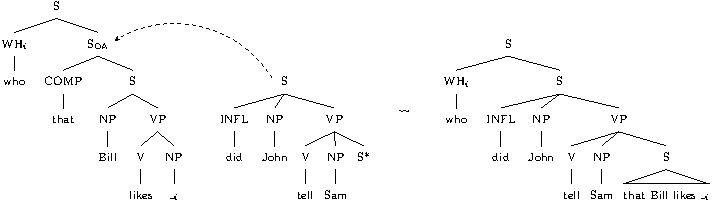
\includegraphics[width=\textwidth]{Figures/tag-long-distance-dependencies-crop}

%% \oneline{%
%% \begin{forest}
%% tag
%% [S
%% 	[WH$_i$
%% 		[who]]
%% 	[%\tikzmark{soa}{S\sub{OA}}
%%          S\sub{OA},name=soa
%% 		[COMP
%% 			[that]]
%% 		[S
%% 			[NP
%% 				[Bill]]
%% 			[VP
%% 				[V
%% 					[likes]]
%% 				[NP
%% 					[\noexpand\_$_i$]]]]]]
%% \end{forest}
%% %}
%% %\hspace{0.5cm}
%% \qquad
%% %\scalebox{.5}{%
%% \begin{forest}
%% tag
%% [S,name=s%\tikzmark{s}{S}
%% 	[INFL
%% 		[did]]
%% 	[NP
%% 		[John]]
%% 	[VP
%% 		[V
%% 			[tell]]
%% 		[NP
%% 			[Sam]]
%% 		[S*]]]
%% \end{forest}
%% %}
%% \qquad \raisebox{2cm}{$\rightsquigarrow$} \qquad
%% %\scalebox{.5}{%
%% \begin{forest}
%% tag
%% [S
%% 	[WH$_i$
%% 		[who]]
%% 	[S
%% 		[INFL
%% 			[did]]
%% 		[NP
%% 			[John]]
%% 		[VP
%% 			[V
%% 				[tell]]
%% 			[NP
%% 				[Sam]]
%% 			[S
%% 				[that Bill likes \noexpand\_$_i$, roof]]]]]
%% \end{forest}
%% \begin{tikzpicture}[overlay,remember picture]
%% \draw[->, dashed, bend angle=45, bend right] ($(pic cs:s)+(-0.25,0.2)$) to($(pic cs:soa)+(0.8,.2)$);
%% \end{tikzpicture}
%% }

\vfill

\eal
\ex \blaubf{who$_i$} did John tell Sam \blaubf{that Bill likes \_$_i$}\\
\pause
\ex \blaubf{who$_i$} did John tell Sam that Mary said \blaubf{that Bill likes \_$_i$}
\zl

\vfill



}

\frame{
\frametitle{Noch einige Details}

\begin{itemize}
\item Der Baum für \emph{WH COMP NP likes \_$_i$} gehört zur Baumfamilie von \emph{likes} und steht
  somit im Lexikon.
\item Obwohl der Baum für (\mex{1}) die Kategorie S hat, ist (\mex{1})  kein grammatischer
  Satz des Englischen.
\ea[*]{
who that Bill likes
}
\z
\pause
Die Markierung OA sagt, daß an der entsprechenden Stelle eine obligatorische Adjunktion stattfinden
muß.

\end{itemize}


}


\frame{
\frametitle{Idiome in TAG}

Idiom-Analyse ganz einfach. \citet{AS89a}:

\centerline{
\scalebox{.9}{%
\begin{forest}
tag
[S
	[NP$\downarrow$]
	[VP
		[V
			[takes]]
		[NP$\downarrow$]
		[PP$_{{\mathrm{NA}}}$
			[P
				[into]]
			[NP$_{\mathrm{NA}}$
				[N$_{\mathrm{NA}}$
					[account]]]]]]
\end{forest}
}}

}



%% -*- coding:utf-8 -*-

\section{Minimalism}

\outline{

\begin{itemize}
\item Begriffe
\item Phrasenstrukturgrammatiken
\item Government \& Binding (GB)
\item Generalisierte Phrasenstrukturgrammatik (GPSG)
\item Lexikalisch-Funktionale Grammatik (LFG)
%\item Lexical Mapping Theory (LMT)
%\item PATR
\item Kategorialgrammatik (CG)
\item Kopfgesteuerte Phrasenstrukturgrammatik (HPSG)
\item Konstruktionsgrammatik (CxG)
\item Baumadjunktionsgrammatik (TAG)
\item \blaubf{Minimalism}
\end{itemize}
}


\frame{
\frametitle{Minimalismus}


\begin{itemize}
\item wie GB durch Noam Chomsky am MIT in Boston entwickelt \citeyearpar{Chomsky93b-u,Chomsky95a-u}
\item Problem der Evolution von Sprache: Wenn sprachspezifisches Wissen in unserem Genom kodiert
  ist, wie ist es da hingekommen?
\item Also möglichst minimale Annahmen bezüglich angeborenem sprachspezifischem Wissen \citep*{HCF2002a}
 
\item International weit verbreitet. Eigene Infrastruktur an Zeitschriften, Konferenzen usw.

\item Deutschland: 
      \begin{itemize}
      \item Artemis Alexiadou, Humboldt-Universität zu Berlin; 
      \item Günther Grewendorf, Frankfurt am Main; 
      \item Joseph Bayer, Konstanz; 
      \item Gereon Müller, Leipzig.
      \end{itemize}
\end{itemize}
\nocite{Grewendorf2002a}

}

\frame{
\frametitle{Minimalismus}


\begin{itemize}
\item GB und \xbar-Analysen finden sich in vielen anderen Theorien wieder (GPSG, LFG, HPSG, TAG),
  das ist bei Minimalistischen Analysen seltener der Fall.
\item Es gibt aber interessante Arbeiten, die man auch lesen und verstehen können muss.

\item Explosion von Varianten nach 1993. 
\begin{itemize}
\item \citet{Kayne94a-u}
\item \citet{Rizzi97a-u}: Kartographie
\item \citet{Borer2003a-u,Borer2005a-u}: Exoskeletale Ansätze
\item \citet{Starke2009a}: Nanosyntax
\end{itemize}

Das Folgende basiert auf \citew{Adger2003a}.

\item Lehrbücher: \citet*{Adger2003a,Radford97a-u,HNG2005a} (Vorsicht, Haltbarkeitsdatum evtl.\ überschritten)

\item Übersichtsartikel: \citet{Richards2015a}

\end{itemize}
\nocite{Grewendorf2002a}

}

\subsection{Allgemeines zum Repräsentationsformat}

\frame{
\frametitle{Allgemeines zum Repräsentationsformat}

\begin{itemize}
\item nur zwei Regeln: External Merge und Internal Merge
\item External Merge = Multiplikationsregel der Kategorialgrammatik bzw. Kopf-Komplement-Schema und
  Spezifikator-Kopf Schema der HPSG \citep{BE95a,MuellerUnifying}

\item Internal Merge = Füller-Kopf-Schema der HPSG \citep{MuellerUnifying}

\item Anders als bei CG und HPSG gibt es aber viele, viele Zusatzannahmen.

\end{itemize}

}
\frame{
\frametitle{Architektur}

\begin{itemize}
\item Es gibt keine Tiefenstruktur und Oberflächenstruktur mehr.
\item Kombination und Bewegung sind verwoben.

\medskip

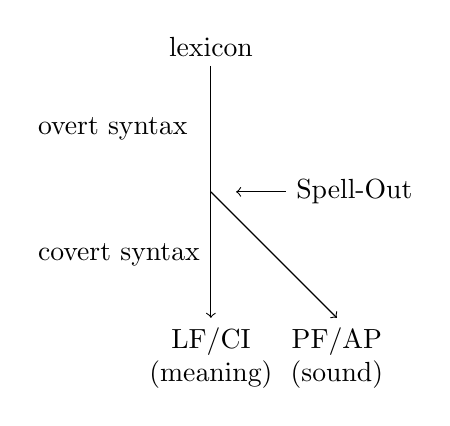
\begin{tikzpicture}[scale=.8]
%\draw (-2.9,-5.8) to[grid with coordinates] (2.7,-0.6);
\draw[->] (0,-1) node[anchor=south] {lexicon} --(0,-5) node[anchor=north, align=center] {LF/CI\\(meaning)};
\draw[->] (0,-3)--(2,-5) node[anchor=north,align=center] {PF/AP\\(sound)};
\draw[<-] (.4,-3)--(1.2,-3) node[anchor=west] {Spell-Out};
%\draw (0,-0.5) node {lexicon};
\draw (-2.9,-2) node[anchor=west] {overt syntax};
\draw (-2.9,-4) node[anchor=west] {covert syntax};
%\draw (0,-6.5) node[align=center] {LF/CI\\(meaning)};
%\draw (2,-5.5) node[align=center] {PF/AP\\(sound)};
\end{tikzpicture}
\end{itemize}

}

\frame{
\frametitle{Phases}

\begin{itemize}
\item Phases: \citet{Chomsky2008a}.
\item Phase is spelled out once it is combined with a head.

\ea
He believes that Peter comes.
\z
\end{itemize}

}


\subsubsection{Valenz, Merkmalsüberprüfung und Agree}
\label{sec-features-minimalism}



\frame{
\frametitle{DP vs.\ NP}


\begin{itemize}
\item Standardannahme im Minimalismus:\\
      \emph{this man} ist eine DP (weil D der Kopf ist, nicht N)

\ea
letters to this man
\z

\pause
\item \emph{him} hat Distribution wie DP, also dieselbe Kategorie:

\ea
letters to him
\z

\end{itemize}
}

\frame{
\frametitle{Valenzrepräsentation über uninterpretierbare Merkmale}


\begin{forest}
baseline
[N 
  [\emph{letters} {[N, pl, \st{\textit{u}P}]}]
  [P
    [\emph{to} {[P, \st{\textit{u}D}]}]
    [\emph{him} {[D]}]]]
\end{forest}

\begin{itemize}
\item \textit{u}D bedeutet, dass ein D gefunden werden muss.
\pause
\item \st{\textit{u}D} bedeutet, dass ein D gefunden wurde.
\end{itemize}

}

\frame{
\frametitle{Valenzrepräsentation und Crash}

\begin{forest}
baseline
[N 
  [\emph{letters} {[N, pl, \st{\textit{u}P}]}]
  [\emph{to} {[P, \textit{u}D]}]]
\end{forest}

\begin{itemize}
\item Objekt ist nicht wohlgeformt, weil \textit{u}D übrig ist.
\item Derivation "`crasht"' an den Interfaces
\end{itemize}

}



\frame[shrink=10]{
\frametitle{Merkmalsüberprüfung mittels Agree}

\eal
\ex[*]{
letters to he
}
\ex[]{
letters to him
}
\zl

\centerline{
\begin{forest}
baseline
[N 
  [\emph{letters} {[N, pl, \st{\textit{u}P}]}]
  [P
    [\emph{to} {[P, \st{\textit{u}D}, \st{acc}]}]
    [\emph{him} {[D, \st{acc}]}]]]
\end{forest}
}

\begin{itemize}
\item Selektionsmerkmale sind atomar, \dash man kann nicht DP[\type{acc}] verlangen.
\item weiterer Mechanismus, der andere Merkmale überprüfen kann: \emph{Agree}
\item über Agree geprüfte Merkmale müssen nicht unbedingt am obersten Knoten präsent sein.
\end{itemize}

}



\subsubsection{Phrasenstruktur und \xbart}

\frame{
\frametitle{Phrasenstruktur und \xbart}

\centerline{
\begin{forest}
%where n children=0{}{},
%sm edges
%for tree={parent anchor=south, child anchor=north,align=center,base=bottom}
[XP
  [specifier]
  [\xbar
    [specifier]
    [\xbar
      [complement] [X] ] ] ]
\end{forest}
}

\begin{itemize}
\item Ob etwas \xbar oder XP ist, hängt davon ab, ob es als Argument benutzt wird oder nicht.
\item vermeidet unschöne unären Verzweigungen der \xbart
\item Probleme: \citew[Abschnitt~2.1]{Brosziewski2003a-u}. 
\end{itemize}

}


\subsubsection{Little \textit{v}}
\label{sec-little-v}

\frame{

\frametitle{Little \textit{v}}

\eal
\ex[*]{
Emily showed himself Benjamin in the mirror.
}
\ex[]{
Peter showed himself Benjamin in the mirror.
}
\zl

\begin{itemize}
\item \emph{himself} kann sich auf Emily, aber nicht auf Benjamin beziehen.

\item \emph{himself} muss höher im Baum sein.
\end{itemize}

}

\frame{
\frametitle{c-command-Anforderungen und ditransitive Verben}

\ea
A node A c-commands B if, and only if A's sister either:\\
\begin{tabular}[t]{@{}l@{~}l@{}}
a. & is B, or\\
b. & contains B
\end{tabular}
\z

\oneline{
\begin{forest}
baseline
[\vbar
 [\textit{show}]
 [\textit{himself}]
 [\textit{Benjamin}]]
\end{forest}
\hfill
\begin{forest}
baseline
[\vbar
   [\vbar
     [\textit{show}]
     [\textit{himself}] ]
 [\textit{Benjamin}]]
\end{forest}
\hfill\hfill
\begin{forest}
baseline
[\littlevbar
 [\textit{show}]
 [VP
   [\textit{himself}]
   [\vbar
    [V]
    [\textit{Benjamin}]]]]
\end{forest}
}
}

\frame{
\frametitle{Ditransitive Verben}

\ea[]{
Peter showed himself Benjamin in the mirror.
}
\z


\begin{itemize}
\item Analyse mit zusätzlichem leeren Verb geht zurück auf \citet{Larson88a}
\item \citet[\page 70]{HK93a-u}: Leeres Verb steuert Kausativsemantik bei.
\item \emph{show} steht in der V-Position und bewegt sich dann zu \textit{v}.
\item \emph{show} bedeutet \emph{see} und bei \littlev kommt dann die kausative Bedeutung dazu,
  woraus sich \relation{cause-see} ergibt \citep[\page 133]{Adger2003a}. 
\end{itemize}

}

\frame{
\frametitle{Ditransitive Verben}
\centerline{
\begin{forest}
baseline
[\vP
  [\textit{Peter}]
  [\littlevbar
   [\textit{v} $+$ \textit{show}]
   [VP
     [\textit{himself}]
     [\vbar
      [\phonliste{ show } {[V]}]
      [\textit{Benjamin}]]]]]
\end{forest}
}
}


\subsubsection{Linking}

\frame{
\frametitle{Little \textit{v} everywhere}

\begin{itemize}
\item Verb-Shell-Analyse ursprünglich nur für ditransitive Verben \citep{Larson88a},\\
 jetzt aber auch für strikt transitive Verben und intransitive Verben verwendet.

\item \citet[Abschnitt~4.5]{Adger2003a}: semantische Rollen einheitlich vergeben:
\eal
\ex DP Tochter von \vP $\to$ interpretiert als agent
\ex DP Tochter von VP $\to$ interpretiert als theme
\ex PP Tochter von \littlevbar $\to$ interpretiert als goal
\zl
\item Adger: einheitlich zugewiesene Rollen helfen bei Spracherwerb,\\
      also \littlev auch bei strikt transitiven und intransitiven Verben.

\item Frage: Involviert \emph{schlafen} eine kausative Komponente? Ein Agens?

\end{itemize}
}

\frame{
\frametitle{Transitive und intransitive Verben}

\vfill
\hfill\begin{forest}
baseline
[\vP
  [Agent]
  [\littlevbar~{[\st{\textit{u}D}]}
   [\textit{v}]
   [VP
      [\textit{burn} {[V, \st{\textit{u}D}]}]
      [Theme]]]]]
\end{forest}
\hfill
\begin{forest}
baseline
[\vP
  [Agent]
  [\littlevbar~{[\st{\textit{u}D}]}
   [\textit{v} ]
   [ \textit{laugh} {[V]} ]]]
\end{forest}
\hfill\mbox{}

\vfill
\begin{itemize}
\item \citet[\page 164]{Adger2003a}:\\
      Auch intransitive und transitive Verben bewegen sich von V nach \textit{v}.
\end{itemize}
\vfill
}

\subsubsection{CP, TP, \vP, VP}
\label{sec-CP-TP-vP-VP}


\subsubsubsection{Merkmale als Auslöser von Bewegungen: Das EPP-Merkmal von T}
\label{sec-epp-features}

\frame{
\frametitle{Merkmale als Auslöser von Bewegung: EPP-Merkmal bei T}

\begin{itemize}
\item In GB waren die Subjekte Spezifikatoren von IP.
\item Jetzt sind sie Spezifikatoren von \vP.
\item Kombiniert man Modalverben mit \vP, steht Subjekt an falscher Stelle.
\eal
\ex[*]{
Will Ann read the book.
}
\ex[]{
Anna will read the book.
}
\zl

\item Annahme eines starken, uninterpretierbaren Merkmals D beim T-Kopf.

\item Starke Merkmale lösen Bewegung aus, weil die Überprüfung lokal erfolgen muss. 
      Sie werden durch ein `*' gekennzeichnet.

\item Da das Merkmal stark ist, muss ein passendes D in die Spezifikatorposition von T bewegt werden
  und das D checken.


\end{itemize}

}

\frame{
\frametitle{Merkmale als Auslöser von Bewegung: EPP-Merkmal bei T}

\centerline{
\scalebox{.8}{%
\begin{forest}
baseline
[TP
 [\textit{Anna} {[D]}]
 [\tbar{[\st{\textit{u}D*}]}
   [\textit{will} T{[pres]}]
   [\vP
     [\phonliste{ Anna }]
     [\littlevbar~{[\st{\textit{u}D}]}
       [\textit{v}
         [\textit{read}] [\textit{v}]]
       [VP
         [\phonliste{ read } {[V, \st{\textit{u}D}]}]
         [DP [\textit{the book}, roof]]]]]]]
\end{forest}
}
}

}

\frame{
\frametitle{EPP: Extended Projection Principle}

\begin{itemize}

\item Das Merkmal wird EPP-Merkmal genannt.\\
      EPP steht für Extended Projection Principle.
\pause

\item EPP gab es schon in der GB: Jeder Satz muss ein Subjekt haben.
\pause

\item Das ist für das Deutsche falsch:
\eal
\ex Mir ist schlecht.
\ex weil noch gearbeitet wurde
\zl

\pause
\item Man kann behaupten, dass in (\mex{0}) leere Subjekte vorliegen,\\das Prinzip wird dadurch aber entwertet.
\end{itemize}
}


\frame{
\frametitle{Komplette Analyse eines Deklarativsatzes mit CP}

\centerline{
\scalebox{.75}{%
\begin{forest}
baseline
[CP
 [C{[Decl]}]
 [TP
 [\textit{Anna} {[D]}]
 [\tbar{[\st{\textit{u}D*}]}
   [\textit{will} T{[pres]}]
   [\vP
     [\phonliste{ Anna }]
     [\littlevbar~{[\st{\textit{u}D}]}
       [\textit{v}
         [\textit{read}] [\textit{v}]]
       [VP
         [\phonliste{ read } {[V, \st{\textit{u}D}]}]
         [DP [\textit{the book}, roof]]]]]]]]
\end{forest}
}
}

}

\frame{
\frametitle{Fragen}

\begin{itemize}
\item Für (\mex{1}) braucht man ein unvalued Satztypen-Merkmal bei T für den Satztyp \emph{question}. 
\ea
What will Anna read?
\z
\item Der leere Komplementierer C hat ein Q-Merkmal, das dem Satztyp-Merkmal bei T einen Wert
  zuweisen kann. (value the feature)
\item Da das Satztypmerkmal bei T strong ist, muss sich das T-Element zu C bewegen, um das Merkmal
  lokal checken zu können.

\item \emph{wh}-Element muss auch bewegt werden. Das wird durch starkes \emph{wh}-Merkmal bei C
  erzwungen.

\end{itemize}

}

\frame{
\frametitle{Fragen: \emph{What will Anna read?}}

\centerline{
\scalebox{.7}{
\begin{forest}
baseline
[CP
 [\textit{what} {[D, wh]}]
 [\cbar{[\st{\textit{u}wh*}]}
   [C
     [\textit{will} T{[\st{Q*}]}]
     [C{[Q]}] ]
   [TP
   [\textit{Anna} {[D]}]
   [\tbar{[\st{\textit{u}D*}]}
     [\phonliste{ will } {[T]}]
     [\vP
       [\phonliste{ Anna }]
       [\littlevbar~{[\st{\textit{u}D}]}
         [\textit{v}
           [\textit{read}] [\textit{v}]]
         [VP
           [\phonliste{ read } {[V, \st{\textit{u}D}]}]
           [\phonliste{what}]]]]]]]]
\end{forest}
}
}
}

\subsubsection{Kasuszuweisung}


\frame{
\frametitle{Kasuszuweisung}

\begin{itemize}
\item Die DPs \emph{Anna} und \emph{the book} haben zu Beginn uninterpretierbare Kasusmerkmale:
[\textit{u}case:]. 
\pause
\item Die Merkmale werden valuiert durch T und \textit{v}.
\pause
\item Nur ein Merkmal wird durch Merge gecheckt. Bei T das D-Merkmal. 
\pause
\item Kasusmerkmal muss mittels eines anderen Checking-Mechanismuses gecheckt werden: Agree.
\pause
\item Agree kann Merkmale in Schwesterknoten checken oder auch weiter weg im Baum.
\pause
\item Knoten muss den Knoten, mit dem es eine Agree-Relation geben soll, c-kommandieren.

\end{itemize}

}

\frame[shrink]{
\frametitle{Kasuszuweisung}

\centerline{
\scalebox{.7}{
\begin{forest}
baseline
[TP
 [\textit{Anna} {[D, \st{nom}]}]
 [\tbar{[\st{\textit{u}D*}, \st{nom}]}
   [T{[pres]}]
   [\vP
     [\phonliste{ Anna }]
     [\littlevbar~{[\st{\textit{u}D}]}
       [\textit{v}
         [\textit{read}] [\textit{v} {[\st{acc}]}]]
       [VP
         [\phonliste{ read } {[V, \st{\textit{u}D}]}]
         [DP{[\st{acc}]} [\textit{the book}, roof]]]]]]]
\end{forest}
}}

\begin{itemize}
\item \textit{v} c-kommandiert VP, V, die DP \emph{the book} und alle Knoten in dieser DP.
\item Da Agree Merkmale von c-kommandierten Knoten valuieren kann,\\
      kann der Akkusativ bei \textit{v} das Kasus-Merkmal der DP \emph{the book} valuen.
\end{itemize}

}


\frame[shrink]{
\frametitle{Nichtlokalität von Agree}

\begin{itemize}
\item Agree kann nicht-lokal Merkmale überprüfen. Aber was ist mit (\mex{1})?
\ea[*]{
\label{ex-him-likes-she}
Him likes she.
}
\z
Der Akkusativ von \textit{v} könnte mit dem Subjekt abgeglichen werden und der Nominativ von T mit
dem Objekt von \emph{likes}.

\centerline{
\scalebox{.7}{
\begin{forest}
baseline
[TP
 [\textit{him} {[D, \st{acc}]}]
 [\tbar{[\st{\textit{u}D*}, \st{nom}]}
   [T{[pres]}]
   [\vP
     [\phonliste{ him }]
     [\littlevbar~{[\st{\textit{u}D},\st{acc}]}
       [\textit{v}
         [\textit{read}] [\textit{v} {[\st{acc}]}]]
       [VP
         [\phonliste{ read } {[V, \st{\textit{u}D}]}]
         [DP{[\st{nom}]} [\textit{she}]]]]]]]
\end{forest}
}}


\end{itemize}
}

\frame{
\frametitle{Nichtlokalität von Agree}

\begin{itemize}
\item Anforderung an Agree: Nimm das nächstmögliche Element.
\item \citet[\page 218]{Adger2003a}:
\ea
\label{principle-locality-of-matching}
Locality of matching\is{locality!of matching}: Agree holds between a feature F on X and a matching feature F on Y if and only
if there is no intervening Z[F].
\z
Intervention ist wie folgt definiert:
\ea
\label{def-intervention}
Intervention\is{intervention}: In a structure [X \ldots{} Z \ldots{} Y], Z intervenes between X and Y iff X
c-commands\is{c"=command} Z and Z c-commands Y.
\z
\item Weil T mit \emph{Anna} Agreen kann, darf es nicht mit \emph{the book} Agreen.
\end{itemize}
}

\subsubsection{Adjunkte}

\frame{
\frametitle{Adjunkte}

\begin{itemize}
\item \citet[Section~4.2.3]{Adger2003a} nimmt an, dass Adjunkte sich mit XP verbinden und eine neue XP
bilden.
\item Er nennt diese Operation \emph{Adjoin}.

\item Operation konsumiert keine Merkmale, ist also anders als External Merge.

\item Das heißt, neue zusätzliche Operation in der Theorie (nicht nur die beiden Merges!).

\item Es gibt Vorschläge, Adjunkte als Elemente innerhalb spezieller adverbieller Phrasen mit leeren
  Köpfen zu behandeln.

\item Ich finde Adgers Lösung besser.\\
      Entspricht dem, was in vielen anderen Frameworks auch gemacht wird.
\end{itemize}

}


\subsection{Verbstellung}
\label{sec-verb-position-MP}

\frame{
\frametitle{Verbstellung}

\begin{itemize}
\item Finites Verb bewegt sich von V zu \textit{v} zu T und dann zu C.
\item Die Bewegung zu T wird durch ein starkes Tense-Merkmal von T erzwungen.
\item Die Bewegung des T-Komplexes nach C wird durch ein Satztypmerkmal ausgelöst, das durch ein
  starkes Interrogativ-Merkmal (Int) bzw. durch ein Deklarativ-Merkmal (Decl) valuiert wird.
\end{itemize}


%% \ea
%% Kennt jeder diesen Mann?
%% \z

}

\frame{
\frametitle{Verbstellung: \emph{Kennt jeder diesen Mann?}}


\scalebox{.7}{
\begin{forest}
[CP
    [C
      [T{[\st{Int*}]}
        [\textit{kennt} {[\st{Pres*}]}]
        [T{[Pres]}]]
      [C{[Int]}]]
    [TP
      [\textit{jeder}]
      [\tbar{[\st{\textit{u}D*}]}
        [\vP
          [\phonliste{ jeder }]
          [\littlevbar
            [VP
              [DP [\textit{diesen Mann}, roof] ]
              [\phonliste{ kennt }]]
            [\textit{v}
              [\phonliste{ kennt }]
              [\textit{v}]]]]
        [\phonliste{ kennt T }]]]]
\end{forest}
}
}


\subsection{Fernabhängigkeiten}

\frame{
\frametitle{Fernabhängigkeiten}

\begin{itemize}
\item Decl bei C löst Verbumstellung aus.
\item Merkmal top löst Bewegung nach SpecCP aus.
\end{itemize}
}

\frame{
\frametitle{Fernabhängigkeiten \emph{Diesen Mann kennt jeder.}}

\scalebox{.7}{
\begin{forest}
[CP
  [\emph{diesen Mann} {[top] }]
  [\cbar{[\st{\textit{u}top*}]}
    [C
      [T{[\st{Decl*}]}
        [\textit{kennt} {[\st{Pres*}]}]
        [T{[Pres]}]]
      [C{[Decl]}]]
    [TP
      [\textit{jeder}]
      [\tbar{[\st{\textit{u}D*}]}
        [\vP
          [\phonliste{ jeder }]
          [\littlevbar
            [VP
              [\phonliste{ diesen Mann }{[D]}]
              [\phonliste{ kennt }]]
            [\textit{v}
              [\phonliste{ kennt }]
              [\textit{v}]]]]
        [\phonliste{ kennt T }]]]]]
\end{forest}
}
}


\subsection{Passiv}

\frame{
\frametitle{Passiv}


\begin{itemize}
\item Wie bei GB weist Verb keinen Akk zu: \littlev hat kein acc-Merkmal.
\item Dafür spezielle Version von \littlev, das auch bei den unakkusativischen Verben eine Rolle spielt \citep{Perlmutter78}.

\citet[\page 140]{Adger2003a}: \vPs für unakkusativische Verben \emph{fall}, \emph{collapse}, \emph{wilt}:

\vfill

\begin{forest}
[\vP
  [\textit{v}]
  [VP
    [\textit{fall}{[V, \textit{u}D]}]
    [Theme]]]
\end{forest}

\vfill

\item Unakkusativisches \littlev spielt auch bei Analyse des Passivs eine Rolle.
\item Es gibt ein Subjekt, das irgendwie Objekteigenschaften hat.
\item Das spezielle \littlev wird von einem Passivkopf \emph{werden} gefordert und\\
      bildet eine Passive Phrase.

\end{itemize}

}

\frame{
\frametitle{Passiv: \emph{dass er geschlagen wurde}}

\centerfit{
%\begin{sideways}  
\begin{forest}
for tree={fit=rectangle}
[TP
     [PassP
       [\vP
         [VP
           [pronoun {[\st{nom}]} ]
           [\phonliste{schlagen}]]
         [\textit{v}
           [\textit{schlagen}]
           [{\textit{v}[\st{\textit{u}Infl}:Pass]}]]]
       [\phonliste{werden}]]
     [{T[past,\st{nom}]}
       [\textit{werden} {[Pass,\st{\textit{u}Infl}:past*]}]
       [{T[past]}]]]
\end{forest}
%\end{sideways}
}

\begin{itemize}
\item Pass-Kopf verlangt Infl-Merkmal von \littlev mit Wert Pass.
\item Partizip-Morphologie bei Spell-Out.
\item Hilfsverb bewegt sich zu T, um starkes Infl zu checken.
\item Weil Infl-Wert past ist, muss Form \emph{wurde} ausgesprochen werden
\item Es gibt keine Bewegung! Kasus wird über Agree vergeben.
\end{itemize}


}

\frame{
\frametitle{Passiv: Aber}

\begin{itemize}
\item Das ist besser als bei der GB-Analyse mit IP.
\item Aber: \citet[\page 332]{Adger2003a} nimmt für Deutsch an, dass es ein starkes EPP-Merkmal
  gibt.
\item Daraus ergeben ich dieselben Probleme wie beim GB-Ansatz.
\item Alle Objekte müssen sich zu T bewegen, auch wenn es keine Umstellung im Satz gibt.
\item Unpersönliche Passive sind problematisch, da es nichts gibt,\\
      was sich zu T bewegen könnte.
\ea
weil getanzt wurde
\z
\end{itemize}
}


\subsection{Lokale Umstellung}

\frame{
\frametitle{Lokale Umstellung}

\begin{itemize}
\item \citet{Adger2003a} behandelt Scrambling nicht.
\item Alle Umordnungen sind merkmalsgesteuert, also muss es irgendein Merkmal geben, das
  Umstellungen wie in (\mex{1}b) auslöst:
\eal
\ex 
{}[weil] jeder diesen Mann kennt
\ex 
{}[weil] diesen Mann jeder kennt
\zl
\item Diverse Vorschläge in der Literatur mit so genannten funktionalen Projektionen:
\begin{itemize}
\item Topic Phrase \citep[\page 222]{Laenzlinger2004a} 
\item AgrS und AgrO \citep[Kapitel~4]{Meinunger2000a}
\end{itemize}
\item Bessere Lösung von G.\ \citet[Abschnitt~3.5]{GMueller2014a-u}:
      Objekt bewegt sich zu zweiter Spezifikatorposition von \littlev. 
\item Dazu werden optionale Merkmale bei \textit{v} und V angenommen (S.\,48).
\end{itemize}
} 

\frame{
\frametitle{Lokale Umstellung \emph{dass diesen Mann jeder kennt}}

\scalebox{.8}{
\begin{forest}
[CP
    [C
      [dass]]
    [TP
        [\vP
          [\emph{diesen Mann}]
          [\littlevbar
            [ \emph{jeder}]
            [\littlevbar
                [VP
                  [\phonliste{ diesen Mann } {[D]}] 
                  [\phonliste{ kennt }]]
                [\textit{v}
                  [\phonliste{ kennt }]
                  [\textit{v}]]]] ]
        [\textit{kennt} {[T]}]]]
\end{forest}
}

}

\frame{
\frametitle{Überblick über Stipulationen}

\begin{itemize}
\item Annahmen in Adgers Analyse:
\begin{itemize}
\item Kategorie eines Knotens hängt davon ab, wie er verwendet wird (noch erweitert oder nicht).
\item Bei Merge kann immer genau ein Merkmal überprüft werden.
\item Andere Merkmale werden mit Agree überprüft.
\item Agree kann Merkmale überprüfen, wenn c-Kommando vorliegt.
\item Agree kann nur dann Merkmale überprüfen, wenn kein anderes Merkmal interveniert.
\item Es gibt starke und schwache Merkmale.
\item Derivationen, die noch Merkmale übrig haben, crashen an den Interfaces.
\end{itemize}
\pause
\item Es gibt ein Spracherwerbsproblem.
\pause
\item Zum Vergleich CG und HPSG:
\begin{itemize}
\item Es gibt einen Funktor mit einer Beschreibung des abhängigen Elements.
\item Abhängiges Element muss passen.
\end{itemize}
\pause
\item Adgers Analyse ist die MP-Analyse mit den wenigsten Stipulationen.
\end{itemize}


}

\subsection{Varianten und Argumentation für Theorien}

\frame{
\frametitle{Varianten und Argumentation für Theorien}

\begin{itemize}
\item Es gibt viele Varianten und Sub-Schulen.
\item Kartographie (Crypto-Konstruktivismus): Probleme mit der Syntax-Semantik-Trennung werden durch
  Syntaktifizierung der Semantik umgangen \citep{Rizzi2014a}
\item Kaynesche Ansätze mit zugrundeliegender Specifier-Head-Complement-Anordnung für alle Sprachen.
\item \ldots
\end{itemize}


}

\frame{
\frametitle{Varianten: \citet{Rizzi97a-u}}

\scalebox{.5}{%
\newlength\mytextheight
\settototalheight{\mytextheight}{XpX$^0$X$'$}
\begin{forest}
  delay={
    where content={}{
      content={\phantom{X}}
    }{},
  },
  for tree={
    text height=\mytextheight,
    fit=band,
    parent anchor=south,
    child anchor=north,
  }
[ForceP
	[]
	[Force$'$
		[Force$^0$]
		[TopP*
			[]
			[Top$'$
				[Top$^0$]
				[FocP
					[]
					[Foc$'$
						[Foc$^0$]
						[TopP*
							[]
							[Top$'$
								[Top$^0$]
								[FinP
									[]
									[Fin$'$
										[Fin$^0$]
										[IP]]]]]]]]]]]
\end{forest}
}

}


\frame{
\frametitle{Evidence from a single language and UG}


\begin{itemize}
\item What does it mean for other languages\\
      that a rule/morpheme is present in one particular language?
\pause
\item Possible answer:\\
      If we have a certain structure in language X,\\
      it must be present in all languages.
\pause
\item Example:
      \begin{itemize}
      \item Basque: Tree positions for object agreement (AgrO, AgrIO)\nocite{Chomsky93b-u,Stechow96a,Grewendorf2002a,Meinunger2000a}
      \item Japanese/Gungbe: Tree position for topic marker\nocite{CR2010a} %\citet[\page 62]{CR2010a}
      \end{itemize}

\pause
\item German and Dutch neither have object agreement nor topic morphemes.

\pause
\item Conclusion:\\
      If such inferences regarding properties of particular languages are made,\\
      one has to assume (very specific!) innate linguistic knowledge.

\end{itemize}

% Parameter
\nocite{Newmeyer2005a}
}

%% \frame[shrink]{
%% \frametitle{AgrS, AgrIO und AgrO nach \citew[S.\,101]{Meinunger2000a}}

%% \begin{columns}[T]

%% \begin{column}{65mm}
%% \scalebox{0.4}{\begin{pspicture}(1.6,0)(17.4,16.3)
%% %\psgrid
%% %% \only<handout>{\psline[linewidth=5mm,linecolor=red](3,14)(16,1)
%% %% \psline[linewidth=5mm,linecolor=red](3,1)(16,14)}
%% \rput[B](3,0){\rnode{die Firma}{die Firma Müller}}
%% \rput[B](6,0){\rnode{meinem Onkel}{meinem Onkel}}
%% \rput[B](9,0){\rnode{diese Moebel}{diese Möbel}}
%% \rput[B](12,0){\rnode{erst gestern}{erst gestern}}
%% \rput[B](15,0){\rnode{zugestellt}{zugestellt}}
%% \rput[B](17,0){\rnode{hat}{hat}}
%% %
%% \rput[B](14,2){\rnode{tdo}{t\sub{DO}}}
%% \rput[B](15,2){\rnode{v}{V}}
%% \rput[B](14.5,3){\rnode{vp1}{VP}}
%% %
%% \rput[B](13.5,3){\rnode{tio}{t\sub{IO}}}
%% \rput[B](14,4){\rnode{vs}{V'}}
%% %
%% \rput[B](13,4){\rnode{tsu}{t\sub{SU}}}
%% \rput[B](13.5,5){\rnode{vp2}{VP}}
%% %
%% \rput[B](12,5){\rnode{adv}{Adv}}
%% \rput[B](13,6){\rnode{vp3}{VP}}
%% %
%% \rput[B](15,6){\rnode{agro0}{AgrO$^0$}}
%% \rput[B](14,7){\rnode{agros}{AgrO'}}
%% %
%% \rput[B](9,7){\rnode{do}{DO}}
%% \rput[B](11.5,9){\rnode{agrop}{AgrOP}}
%% %
%% \rput[B](13.5,9){\rnode{agrio0}{AgrIO$^0$}}
%% \rput[B](12.5,10){\rnode{agrios}{AgrIO'}}
%% %
%% \rput[B](6,10){\rnode{io}{IO}}
%% \rput[B](9.25,12){\rnode{agriop}{AgrIOP}}
%% %
%% \rput[B](17,12){\rnode{agrs0}{AgrS$^0$}}
%% \rput[B](13.125,14){\rnode{agrss}{AgrS'}}
%% %
%% \rput[B](3,14){\rnode{su}{SU}}
%% \rput[B](8.06125,16){\rnode{agrsp}{AgrSP}}
%% %
%% \psset{angleA=-90,angleB=90,arm=0pt}
%% %
%% \ncdiag{vp1}{v}
%% \ncdiag{vp1}{tdo}
%% %
%% \ncdiag{vs}{tio}
%% \ncdiag{vs}{vp1}
%% %
%% \ncdiag{vp2}{vs}
%% \ncdiag{vp2}{tsu}
%% %
%% \ncdiag{vp3}{vp2}
%% \ncdiag{vp3}{adv}
%% %
%% \ncdiag{agros}{vp3}
%% \ncdiag{agros}{agro0}
%% %
%% \ncdiag{agrop}{agros}
%% \ncdiag{agrop}{do}
%% %
%% \ncdiag{agrios}{agrop}
%% \ncdiag{agrios}{agrio0}
%% %
%% \ncdiag{agriop}{agrios}
%% \ncdiag{agriop}{io}
%% %
%% \ncdiag{agrss}{agriop}
%% \ncdiag{agrss}{agrs0}
%% %
%% \ncdiag{agrsp}{agrss}
%% \ncdiag{agrsp}{su}
%% %
%% \pstriangle(3,0.4)(2.6,13.5)
%% \pstriangle(6,0.4)(2.3,9.5)
%% \pstriangle(9,0.4)(1.9,6.5)
%% \pstriangle(12,0.4)(1.7,4.5)
%% \ncdiag{v}{zugestellt}
%% \ncdiag{agrs0}{hat}
%% %% \only<beamer>{\only<3->{\psline[linewidth=5mm,linecolor=red](3,14)(16,1)
%% %% \psline[linewidth=5mm,linecolor=red](3,1)(16,14)}}
%% \end{pspicture}}
%% \end{column}
%% \begin{column}{55mm}
%% {\footnotesize
%% \begin{itemize}
%% \item Objektkongruenz im Baskischen.

%%       Wir modellieren das mit Baumkonfigurationen. $\to$

%%       Es muss die Konfigurationen in allen Sprachen geben.
%% \pause
%% \item Wenn wir den Baum schon mal haben, können
%%       wir ihn für die Modellierung d.\ Informationsstruktur im Deutschen benutzen.
%% \pause
%% \item Nein! Kongruenz ist eine Eigenschaft der beteiligten Objekte:\\
%%       die Gleichheit von Werten.

%%       Konfigurationale Aspekte sind dabei irrelevant.
%% \end{itemize}
%% }
%% \end{column}
%% \end{columns}

%% }



\frame{
\frametitlefit{Deutsch ist Englisch/Romanisch (SVO, Laenzlinger nach Kayne)}

\nocite{Laenzlinger2004a,Kayne94a-u}
\begin{columns}[T]

\begin{column}{80mm}
\mode<beamer>{%
\scalebox{0.5}{
\small
\psset{xunit=10mm,yunit=6mm}
%
\begin{pspicture}(-0.4,3)(16.2,20.8)
\rput[B](2,20){\rnode{CP}{CP}}
\rput[B](0,18){\rnode{C}{\cnull}}
\rput[B](4,18){\rnode{SubjP}{SubjP}}
\rput[B](2,16){\rnode{SpecSubjP}{\alt<32->{DP}{XP}}}
\rput[B](6,16){\rnode{ObjP}{\ldots ObjP}}
\rput[B](4,14){\rnode{SpecObjP}{\alt<15->{DP}{XP}}}
\rput[B](8,14){\rnode{AuxP}{\ldots AuxP}}
\rput[B](6,12){\rnode{SpecAuxP}{\alt<49->{VP}{XP}}}
\rput[B](10,12){\rnode{AuxPlus}{Aux+}}
\rput[B](8,10){\rnode{Aux}{Aux}}
\rput[B](12,10){\rnode{vP}{$\nu$P}}
\rput[B](10,8){\rnode{SpecvP}{DP}}
\rput[B](14,8){\rnode{VP}{VP}}
\rput[B](12,6){\rnode{V}{\visible<beamer| beamer:-36>{V}}}
\rput[B](16,6){\rnode{ObjDP}{\visible<beamer| beamer:-36>{DP}}}
%
\psset{angleA=-90,angleB=90,arm=0pt}
%
\ncdiag{CP}{C}\ncdiag{CP}{SubjP}
\ncdiag{SubjP}{SpecSubjP}\ncdiag{SubjP}{ObjP}
\ncdiag{ObjP}{SpecObjP}\ncdiag{ObjP}{AuxP}
\ncdiag{AuxP}{SpecAuxP}\ncdiag{AuxP}{AuxPlus}
\ncdiag{AuxPlus}{Aux}\ncdiag{AuxPlus}{vP}
\ncdiag{vP}{SpecvP}\ncdiag{vP}{VP}
%
\rput[B](0,4){\rnode{weil}{weil}}
\rput[B](2,4){\rnode{er-vorn}{\visible<beamer| beamer:-32>{[ \_ ]}}}
\rput[B](4,4){\rnode{ihn-vorn}{\visible<beamer| beamer:-15>{[ \_ ]}}}
\rput[B](6,4){\rnode{gelesen-vorn}{\visible<beamer| beamer:-49>{[ \_ ]}}}
\rput[B](8,4){\rnode{hat}{hat}}
\rput[B](10,4){\rnode{er}{\visible<beamer| beamer:-18>{er}}}
\rput[B](12,4){\rnode{gelesen}{\visible<beamer| beamer:-35>{gelesen}}}
\rput[B](14,4){\rnode{trace-VP}{\visible<beamer| beamer:37->{[ \_ ]$_k$}}}
\rput[B](16,4){\rnode{ihn}{\visible<beamer| beamer:1>{ihn$_j$}}}
%
\ncdiag{C}{weil}
\ncdiag{SpecSubjP}{er-vorn}
\ncdiag{SpecObjP}{ihn-vorn}
\visible<beamer| beamer:-49>{\ncdiag{SpecAuxP}{gelesen-vorn}}
\ncdiag{Aux}{hat}
\ncdiag{SpecvP}{er}

\alt<-36>{
\ncdiag{VP}{V}\ncdiag{VP}{ObjDP}
\ncdiag{V}{gelesen}
\ncdiag{ObjDP}{ihn}
}{
\ncdiag{VP}{trace-VP}
}

\visible<beamer| beamer:50->{\pstriangle(6,4.6)(2,7.2)}
%\pscircle(12,8.5){1.9}
%\psline{->}(12,5.4)(12,5)(6,5)(6,5.6)
%\psline{->}(14,7.8)(14,4)(4,4)(4,5.6)
% 16 * .75 = 12
%  4 * .6  = 2.4
%
% 10 * .75 = 7.5 
%  2 * .75 = 1.5
\tmove<2-17>(16cm,2.4cm)(4cm,2.4cm){ihn$_j$}{\visible<beamer| beamer:-36>{[ \_ ]$_j$}}
\tmove<19-34>(10cm,2.4cm)(2cm,2.4cm){er$_i$}{[ \_ ]$_i$}
% The whole VP is the trace.
\tmove<36-51>(12cm,2.4cm)(6cm,2.4cm){[gelesen [ \_ ]$_j$ ]$_k$}{}
%\psgrid
%
\end{pspicture}
}
}
\mode<handout>{%
\scalebox{0.5}{
\small
\psset{xunit=9mm,yunit=6mm}
%
\begin{pspicture}(-0.4,1)(16.2,20.8)
\rput[B](2,20){\rnode{CP}{CP}}
\rput[B](0,18){\rnode{C}{\cnull}}
\rput[B](4,18){\rnode{SubjP}{SubjP}}
\rput[B](2,16){\rnode{SpecSubjP}{DP}}
\rput[B](6,16){\rnode{ObjP}{\ldots ObjP}}
\rput[B](4,14){\rnode{SpecObjP}{DP}}
\rput[B](8,14){\rnode{AuxP}{\ldots AuxP}}
\rput[B](6,12){\rnode{SpecAuxP}{VP}}
\rput[B](10,12){\rnode{AuxPlus}{Aux+}}
\rput[B](8,10){\rnode{Aux}{Aux}}
\rput[B](12,10){\rnode{vP}{$\nu$P}}
\rput[B](10,8){\rnode{SpecvP}{DP}}
\rput[B](14,8){\rnode{VP}{VP}}
\rput[B](12,6){\rnode{V}{{V}}}
\rput[B](16,6){\rnode{ObjDP}{{DP}}}
%
\psset{angleA=-90,angleB=90,arm=0pt}
%
\ncdiag{CP}{C}\ncdiag{CP}{SubjP}
\ncdiag{SubjP}{SpecSubjP}\ncdiag{SubjP}{ObjP}
\ncdiag{ObjP}{SpecObjP}\ncdiag{ObjP}{AuxP}
\ncdiag{AuxP}{SpecAuxP}\ncdiag{AuxP}{AuxPlus}
\ncdiag{AuxPlus}{Aux}\ncdiag{AuxPlus}{vP}
\ncdiag{vP}{SpecvP}\ncdiag{vP}{VP}
%
\rput[B](0,4){\rnode{weil}{weil}}
\rput[B](2,4){\rnode{er-vorn}{er}}
\rput[B](4,4){\rnode{ihn-vorn}{ihn}}
\rput[B](6,4){\rnode{gelesen-vorn}{gelesen}}
\rput[B](8,4){\rnode{hat}{hat}}
%\rput[B](10,4){\rnode{er}{\visible<beamer| beamer:-18>{er}}}
%\rput[B](12,4){\rnode{gelesen}{\visible<beamer| beamer:-35>{gelesen}}}
%\rput[B](14,4){\rnode{trace-VP}{\visible<beamer| beamer:37->{[ \_ ]$_k$}}}
%\rput[B](16,4){\rnode{ihn}{\visible<beamer| beamer:1>{ihn$_j$}}}
%
\ncdiag{C}{weil}
\ncdiag{SpecSubjP}{er-vorn}
\ncdiag{SpecObjP}{ihn-vorn}
\ncdiag{SpecAuxP}{gelesen-vorn}
\ncdiag{Aux}{hat}
\ncdiag{SpecvP}{er}

\ncdiag{VP}{V}\ncdiag{VP}{ObjDP}
\ncdiag{V}{gelesen}
\ncdiag{ObjDP}{ihn}

\visible<beamer| beamer:50->{\pstriangle(6,4.6)(2,7.2)}
\pscircle(14,6.5){2.3}
\psline{->}(10,7.8)(10,3)(2,3)(2,3.6)
\psline{->}(14,2.6)(14,2)(6,2)(6,3.6)
\psline{->}(16,5.8)(16,1)(4,1)(4,3.6)
%\psgrid
%
\end{pspicture}
}
}
\end{column}
\begin{column}{40mm}
\footnotesize
\begin{itemize}
\item All languages are Spr-H-Comp underlyingly.
\item<2-> The object is moved out of the VP.
\item<19-> The subject is fronted.
\item<36-> The empty VP is fronted.
\item<52-> There are further empty heads \citep{Cinque99a-u}.
\item<53-> Innateness has to be assumed.
\end{itemize}
\end{column}
\end{columns}

\pause
\pause
\pause
\pause
\only<54>{}


\nocite{Haider2000a}
% against remnant movement
\nocite{Fanselow2002a}


}


\frame{
\frametitle{Deutsch ist Deutsch (GB-Varianten, CG, LFG, HPSG, \ldots)}


\centerline{%
\begin{forest}
sm edges
[CP
 [C [weil]]
 [VP
   [NP [er]]
   [V$'$
     [NP [ihn]]
     [V
       [V [gelesen]]
       [V [hat]]]]]]
\end{forest}
\hfill
\begin{forest}
sm edges
[CP
 [C [weil]]
 [VP
   [NP [er]]
   [NP [ihn]]
   [V [gelesen]]
   [V [hat]]]]
\end{forest}
}

\nocite{Fanselow2001a,CJ2005a,BvN98a}

}

%\fi

\frame{
\frametitle{English, German, \ldots{} are Hungarian}
\begin{columns}[T]

\begin{column}{35mm}
\scalebox{0.65}{
\psset{xunit=5mm,yunit=5mm}
\begin{pspicture}(-1.6,0)(8.6,11)
\rput[B](1.5,10){\rnode{AgrP}{\alert<beamer| beamer:1>{AgrP}}}
\rput[B](-1,8){\rnode{SpecAgrP}{\alt<34->{DP}{XP}}}
\rput[B](-1,0){\rnode{mir}{\visible<beamer| beamer:35->{mir$_j$}}}
\rput[B](4,8){\rnode{Agrs}{\alert<beamer| beamer:1>{Agr$'$}}}
\rput[B](2,6){\rnode{Agr}{\alert<beamer| beamer:1>{Agr}}}
\rput[B](2,0){\rnode{Agrw}{\visible<beamer| beamer:-14>{\trace}}}
\rput[B](6,6){\rnode{PP}{PP}}
\rput[B](6,4){\rnode{Ps}{P$'$}}
\rput[B](4,2){\rnode{P}{P}}
\rput[B](4,0){\rnode{in}{\visible<beamer| beamer:-1>{hinter}}}
\rput[B](8,2){\rnode{DP}{DP}}
\rput[B](8,0){\rnode{dS}{\visible<beamer| beamer:-19>{mir}}}
%
\psset{angleA=-90,angleB=90,arm=0pt}
%
\alert<1>{\ncdiag{AgrP}{SpecAgrP}\ncdiag{AgrP}{Agrs}%
\ncdiag{Agrs}{Agr}\ncdiag{Agrs}{PP}%
\ncdiag{Agr}{Agrw}}%
\ncdiag{PP}{Ps}%
\ncdiag{Ps}{P}\ncdiag{Ps}{DP}%
\ncdiag{P}{in}
\ncdiag{DP}{dS}
\visible<33->{\ncdiag{SpecAgrP}{mir}}
%\psgrid
\tmove<2-17>(2cm,0cm)(1cm,0cm){hinter$_i$}{\trace$_i$}
\tmove<19-34>(4cm,0cm)(-0.5cm,0cm){mir$_j$}{\trace$_j$}
\end{pspicture}

}
\end{column}
\begin{column}{85mm}
\begin{itemize}
\item<1-> \citet*[p.\,124]{HNG2005a}: agreement head for the checking of case features
\item<2-> Preposition is moved there.
\item<19-> DP is put into the specifier position of this head.
\item<36-> Evidence for this:\\ Agreement in Hungarian postpositional phrases
\item<37-> English is like Hungarian,\\
      but the movement is invisible.
\end{itemize}
\end{column}
\end{columns}
}


%\if 0
\frame{
\frametitle{Deutsch ist Deutsch, \ldots{} Ungarisch ist Ungarisch}

\begin{columns}[T]

\begin{column}{35mm}
\scalebox{0.7}{
\psset{xunit=5mm,yunit=5mm}
\begin{pspicture}(-1,0)(4.6,5)
\rput[B](2,4){\rnode{PP}{PP}}
\rput[B](0,2){\rnode{P}{P}}
\rput[B](4,2){\rnode{DP}{DP}}
\rput[B](0,0){\rnode{hinter}{hinter}}
\rput[B](4,0){\rnode{mir}{mir}}
%
\psset{angleA=-90,angleB=90,arm=0pt}
%
\ncdiag{PP}{P}\ncdiag{PP}{DP}
\ncdiag{P}{hinter}\ncdiag{DP}{mir}
%\psgrid
\end{pspicture}
}
\end{column}
\begin{column}{85mm}
\begin{itemize}[<+->]
\item A PP is a P together with an NP (or DP).
\item No movement instead of two movements.
\item Structure has five nodes less.
\item Truly minimal!
\item Question: What constitutes an explanation?\\
      Where and how is complexity of language represented?
\end{itemize}
\end{column}
\end{columns}


}


\frame{
\frametitle{Der Schweizer Käse}

\begin{columns}[T]
\begin{column}{55mm}
\scalebox{.8}{%
\begin{forest}
sm edges without translation
[pP
   [p
	[P [with]]
	[p [$\varnothing$]]]
   [AgrOP
	[D [\textbf{me}]]
	[$\overline{\mbox{AgrO}}$
		[AgrO
			[P [t$'$]]
			[AgrO [,phantom  ]]]
		[PP
			[P [t]]
			[D [\textbf{t}]]]]]]
\end{forest}}
\end{column}
\begin{column}{65mm}
\begin{itemize}
\item from another text book:\\
      \citet[\page 452]{Radford97a-u}
\item \citet[\page 549--550]{Sternefeld2006a-u} calls this a Swiss Cheese analysis, but there are more holes (5) than cheese (2).
\end{itemize}
\end{column}
\end{columns}
}


\subsection{Fundamentale Probleme}

\frame{
\frametitle{Fundamentale Probleme: Kopflose Strukturen}


\begin{itemize}
\item Annahme: Es gibt immer einen Kopf und Strukturen sind binär.
\item Problematisch sind NPN-Konstruktionen \citep{Jackendoff2008a,Bargmann2015a,MuellerCxG}:

\eal
\ex Student after student left the room.
\ex
\label{ex-npn-iteration}
Day after day after day went by, but I never found the courage to talk to
her. \citep{Bargmann2015a}
\zl

\item Jackendoff: 
\begin{itemize}
\item Weder N noch P kann sinnvoll als Kopf bezeichnet werden. 
\item \xbart nicht anwendbar.
\item Semantik nicht kompositional.
\end{itemize}

\end{itemize}



}


\frame{
\frametitle{Fundamentale Probleme: Kopflose Strukturen}


\begin{itemize}

\item G.\,\citet{GMueller2011a} schlägt vor, NPN als Reduplikation zu analysieren: Besondere Form der
  Präposition löst Verdopplung aus.

\item Behauptung: Im Deutschen gäbe es keine NPN-Konstruktionen mit Adjektiven. Ist falsch:
\ea
Die beiden tauchten nämlich geradewegs wieder aus dem heimischen Legoland auf, wo sie im
Wohnzimmer, schwarzen Stein um schwarzen Stein, vermeintliche Schusswaffen nachgebaut
hatten.\footnote{
  taz, 05.09.2018, S.\,20
}
\z
\item Außerdem funktioniert Reduplikation nicht für Iteration wie in (\mex{1}).
\ea
Day after day after day went by, but I never found the courage to talk to
her. \citep{Bargmann2015a}
\z


\end{itemize}



}


%\section{Inateness und Gramatiktheorie}


\frame[shrink=10]{
\frametitle{Inateness und Gramatiktheorie}


\begin{itemize}[<+->]
\item Chomskys Hypothese: Sprachliche Fähigkeiten sind angeboren.
\item Spracherwerb: Prinzipien und Parameter\\
Menschen verfügen über ein vorangelegten Satz grammatischer Kategorien und syntaktischer Strukturen.
\item In Abhängigkeit vom sprachlichen Input, den Kinder bekommen, setzen sie bestimmte Parameter
  und je nach Art der Parametersetzung ergibt sich dann die Grammatik des Deutschen, Englischen oder
  Japanischen.
\item Beispiel: Kopfposition initial oder final.

\item Inateness wird in der Grammatiktheorie missbraucht:\\
Man kann von gewissen Dingen einfach annehmen, dass sie Bestandteil der angeborenen Information sind und so ein einfacheres
  Gesamtsystem enthalten. 
\item Beispiel: Objektkongruenz im Baskischen.\\
 Annahme: Die allgemine Fähigkeit, sowas zu erfassen, ist angeboren. $\to$\\
 Es muss entsprechende Strukturen auch im Deutschen geben.
\item Zur Erklärung der Fakten braucht man die Annahme sprachspezifischen angeborenen Wissens aber nicht.
\end{itemize}

}

\frame{
\frametitlefit{Objektkongruenz im Baskischen motiviert AgrO im Deutschen}

\hfill\scalebox{0.4}{%
\begin{pspicture}(1.6,0)(17.4,16.3)
%\psgrid
\rput[B](3,0){\rnode{die Firma}{die Firma Müller}}
\rput[B](6,0){\rnode{meinem Onkel}{meinem Onkel}}
\rput[B](9,0){\rnode{diese Moebel}{diese Möbel}}
\rput[B](12,0){\rnode{erst gestern}{erst gestern}}
\rput[B](15,0){\rnode{zugestellt}{zugestellt}}
\rput[B](17,0){\rnode{hat}{hat}}
%
\rput[B](14,2){\rnode{tdo}{t\sub{DO}}}
\rput[B](15,2){\rnode{v}{V}}
\rput[B](14.5,3){\rnode{vp1}{VP}}
%
\rput[B](13.5,3){\rnode{tio}{t\sub{IO}}}
\rput[B](14,4){\rnode{vs}{V'}}
%
\rput[B](13,4){\rnode{tsu}{t\sub{SU}}}
\rput[B](13.5,5){\rnode{vp2}{VP}}
%
\rput[B](12,5){\rnode{adv}{Adv}}
\rput[B](13,6){\rnode{vp3}{VP}}
%
\rput[B](15,6){\rnode{agro0}{AgrO$^0$}}
\rput[B](14,7){\rnode{agros}{AgrO'}}
%
\rput[B](9,7){\rnode{do}{DO}}
\rput[B](11.5,9){\rnode{agrop}{AgrOP}}
%
\rput[B](13.5,9){\rnode{agrio0}{AgrIO$^0$}}
\rput[B](12.5,10){\rnode{agrios}{AgrIO'}}
%
\rput[B](6,10){\rnode{io}{IO}}
\rput[B](9.25,12){\rnode{agriop}{AgrIOP}}
%
\rput[B](17,12){\rnode{agrs0}{AgrS$^0$}}
\rput[B](13.125,14){\rnode{agrss}{AgrS'}}
%
\rput[B](3,14){\rnode{su}{SU}}
\rput[B](8.06125,16){\rnode{agrsp}{AgrSP}}
%
\psset{angleA=-90,angleB=90,arm=0pt}
%
\ncdiag{vp1}{v}
\ncdiag{vp1}{tdo}
%
\ncdiag{vs}{tio}
\ncdiag{vs}{vp1}
%
\ncdiag{vp2}{vs}
\ncdiag{vp2}{tsu}
%
\ncdiag{vp3}{vp2}
\ncdiag{vp3}{adv}
%
\ncdiag{agros}{vp3}
\ncdiag{agros}{agro0}
%
\ncdiag{agrop}{agros}
\ncdiag{agrop}{do}
%
\ncdiag{agrios}{agrop}
\ncdiag{agrios}{agrio0}
%
\ncdiag{agriop}{agrios}
\ncdiag{agriop}{io}
%
\ncdiag{agrss}{agriop}
\ncdiag{agrss}{agrs0}
%
\ncdiag{agrsp}{agrss}
\ncdiag{agrsp}{su}
%
\pstriangle(3,0.4)(2.6,13.5)
\pstriangle(6,0.4)(2.3,9.5)
\pstriangle(9,0.4)(1.9,6.5)
\pstriangle(12,0.4)(1.7,4.5)
\ncdiag{v}{zugestellt}
\ncdiag{agrs0}{hat}
\end{pspicture}}\hfill\hfill\mbox{}





}

\frame{
\frametitle{Argumente für Inateness}

\begin{itemize}[<+->]
\item Syntaktische Universalien
\item die Tatsache, dass es eine "`kritische"' Periode für den Spracherwerb gibt
\item Fast alle Kinder lernen Sprache, aber Primaten nicht.
\item Kinder regularisieren spontan Pidgin-Sprachen.
\item Lokalisierung in speziellen Gehirnbereichen
\item Angebliche Verschiedenheit von Sprache und allgemeiner Kognition
\item Williams-Syndrom 
\item KE-Familie mit FoxP2-Mutation 
\item Poverty of the Stimulus
\end{itemize}

Siehe hierzu \citew{Pinker94a} und die Kritik von \citew{Tomasello95a}.

}


\subsection{Syntaktische Universalien}


\frame{
\frametitle{Syntaktische Universalien}

Behauptung: Folgende Dinge sind universal und sprachspezifisch:
\begin{itemize}[<+->]
\item \xbar-Strukturen
\item Grammatische Funktionen wie Subjekt und Objekt
\item Eigenschaften von Fernabhängigkeiten
\item Grammatische Morpheme für Tempus, Modus und Aspekt
\item Wortarten (Nomen und Verb)
\item Rekursion \citep*{HCF2002a}
\end{itemize}

}

\subsubsection{\xbar-Strukturen}

\frame{
\frametitle{\xbar-Strukturen}

\begin{itemize}[<+->]
\item Es gibt Sprachen wie Dyirbal (Australien), für die es \zb nicht sinnvoll erscheint, eine VP anzunehmen.

\item Formal ist die Annahme von \xbar-Strukturen keine Einschränkung der möglichen Grammatiken,
wenn man leere Köpfe zuläßt. \citep{KP90a}

\pause
 Im Rahmen des Minimalistischen Programms gibt es eine Inflation leerer Köpfe.

\end{itemize}

}

\subsubsection{Grammatische Funktionen wie Subjekt und Objekt}

\frame{
\frametitle{Grammatische Funktionen wie Subjekt und Objekt}



}

\subsubsection{Eigenschaften von Fernabhängigkeiten}

\frame{
\frametitle{Eigenschaften von Fernabhängigkeiten}

Eine Kernbeschränkung für Bewegung gilt schon nicht für das Deutsche,\\
kann also auch keine universale Beschränkung sein \citep{Mueller2004d}.

}

\subsubsection{Grammatische Morpheme für Tempus, Modus und Aspekt}

\frame{
\frametitle{Grammatische Morpheme für Tempus, Modus und Aspekt}


}

\subsubsection{Wortarten (Nomen und Verb)}

\frame{
\frametitle{Wortarten (Nomen und Verb)}



}

\subsubsection{Rekursion}

\frame{
\frametitle{Rekursion}

\begin{itemize}
\item \citet*{HCF2002a}: Die einzige domänenspezifische Universalie ist Rekursion.
\item Eventuell gibt es Sprachen, die keine Rekursion verwenden:
      \begin{itemize}
      \item Pirah{\~a} \citep{Everett2005a-u}\\
      (siehe jedoch auch \citew*{NPR2009a-u})
      \item Walpiri \citep{Hale76a}
      \end{itemize}
\item Rekursion gibt es auch im nichtsprachlichen Bereich:
      \begin{itemize}
      \item Planung
      \item Stammbäume
      \end{itemize}
\end{itemize}

}

\subsection{Zusammenfassung}

\frame{
\frametitle{Zusammenfassung}

Es gibt keine linguistischen Universalien, bei denen man sich einig ist, dass man
domänenspezifisches angeborenes Wissen braucht.

}


\subsection{Kritische Periode für den Spracherwerb}

\frame{
\frametitle{Kritische Periode für den Spracherwerb}

\begin{itemize}
\item Bei Enten gibt es eine kritische Phase, in der deren Bezugsverhalten geprägt wird.
\item Kinder erlernen Sprache besser als Erwachsene.
\item Es ist jedoch nicht so, dass nach einer bestimmten Zeit der Spracherwerb unmöglich wird.
\item Kein abrupter Übergang wie bei Enten sondern ein stetiger Abfall.
\item Das ist jedoch auch in anderen Domänen beobachtbar:
      \zb ist Autofahren in hohem Alter schwerer erlernbar.
\item Die geringere Gehirnkapazität von Kindern kann zu einer Vereinfachung der Wahrnehmung der
  Input-Daten führen und somit den Kindern beim Spracherwerb helfen. ("`Weniger ist mehr"'-Hypothese) 
\end{itemize}

}

\subsection{Kein Spracherwerb bei Primaten}

\frame{
\frametitle{Kein Spracherwerb bei nichtmenschlichen Primaten}

\begin{itemize}
\item Nichtmenschliche Primaten verstehen Zeigegesten nicht.
\item Menschen imitieren gern.
\item Nichtmenschlichen Primaten könnten die sozialen/kognitiven Voraussetzungen für Sprache fehlen.
\end{itemize}

}


\subsection{Pidgin-Sprachen}

\frame{
\frametitle{Pidgin-Sprachen}

\begin{itemize}
\item Kinder regulasieren Sprache (\zb Pidgin-Sprachen)
\item Dies kann man jedoch als probability matching erklären,\\
      das auch in anderen Domänen auftritt.
\item Beispiel: Zwei Glühlampen, die blinken. Wenn eine in 70\% der Fälle blinkt, können
  Versuchspersonen das vorhersagen.

Bei drei Glühlampen, von denen eine in 70\% der Fälle blinkt und die anderen in je 15\%, sagen die
Probanden 80--90\% für die häufiger blinkende voraus.
\end{itemize}

}

\frame{
\frametitle{Regularisierung}

\begin{itemize}[<+->]
\item Bringt man Versuchspersonen eine künstliche Sprache bei, in der Determinierer in 60\% der Fälle
  ausgedrückt werden, produzieren sie ebenfalls in ca. 60\% der Fälle Determinierer. 

\item Bringt man den Probanden eine Sprache bei, in der zu 60\% ein Determinierer ausgedrückt wird und
  zusätzlich noch weitere Determinierer, die weniger häufig auftreten, dann erzeugen sie den
  Determinierer in mehr als 80\% der Fälle, \dash sie regularisieren. 

\item Kinder regularisieren stärker als Erwachsene.
\item Erinnern Sie sich an die "`Weniger ist mehr"'-Hypothese.
\end{itemize}

}

\subsection{Lokalisierung in speziellen Gehirnbereichen}

\frame{
\frametitle{Lokalisierung in speziellen Gehirnbereichen}

\begin{itemize}
\item Sprachvermögen ist in speziellen Gehirnbereichen lokalisiert.
\item Allerdings können bei Beschädigung auch andere Gehirnbereiche diese Funktion übernehmen.
\item Beim Lesen wird auch ein bestimmter Gehirnbereich aktiviert.\\
Man würde allerdings daraus nie schließen,\\
dass die Fähigkeit zu lesen angeboren ist.
\end{itemize}

}

\subsection{Verschiedenheit von Sprache und allgemeiner Kognition}

\frame{
\frametitle{Verschiedenheit von Sprache und allgemeiner Kognition}

}

\subsection{Williams-Syndrom}

\frame{
\frametitle{Williams-Syndrom}

}

\subsection{KE-Familie mit FoxP2-Mutation}

\frame{
\frametitle{KE-Familie mit FoxP2-Mutation}

}

\subsection{Poverty of the Stimulus}

\frame{
\frametitle{Poverty of the Stimulus}

}

%% -*- coding:utf-8 -*-


\section{Zusammenfassung}


\frame{
\frametitle{Kopflose, idiosynkratische Strukturen}

\begin{itemize}
\item Es gibt Strukturen, die nicht der \xbart entsprechen.

\citet{Matsuyama2004a} und \citet{Jackendoff2008a}:
\eal
\ex Student after student left the room.
\ex
\label{ex-npn-iteration}
Day after day after day went by, but I never found the courage to talk to
her. \citep{Bargmann2015a}
\zl

\pause

\item Diese sind problematisch für CG, DG und Minimalismus, weil diese Theorien einen Kopf/Funktor
  verlangen.

\pause
\item GPSG, LFG, HPSG, CxG, TAG haben damit kein Problem, weil man beliebige Strukturen mit einer
  Bedeutung kombinieren kann.

\end{itemize}


}

\frame{
\frametitle{Übersicht}


\oneline{%
\begin{tabular}{@{}lllll@{}}
Theorie & V1                & V2                     & Passiv       & Scrambling\\
GB      & Bewegung          & Bewegung               & lexikalisch  & Bewegung/Basisgenerierung\\
GPSG    & ID/LP flach       & \slasch                & Metaregel    & ID/LP flach\\
LFG     & co-heads          & functional uncertainty & Lexikonregel & Unterspezifikation von Kasus\\
CG      & direkt/leerer Kopf & Typanhebung \ldots    & Lexikonregel & direkte Kombination\\
HPSG    & \dsl (Kopfbewegung) & \slasch (X(P)-Bewegung) & Lexikonregel  & direkte Kombination\\     
SBCG    & ist HPSG-Variante\\
CxG     & flach?            & flach?                 & Allostruktion & ? Unterspezifikation ID/LP?\\
Minimalism & Bewegung       & Bewegung               & alternatives \textit{v} & Bewegung/Basisgenerierung\\
\end{tabular}}


}

\frame{
\frametitle{Zusammenfassung der gesamten Veranstaltung}

\begin{itemize}
\item Irgendwie machen wir alle dasselbe.
\item Irgendwie dann aber doch nicht.
\end{itemize}



}



\appendix
% mu� immer geladen werden, wegen Referenzen
%\section<presentation>*{Literatur}

%% \frame{
%%   \frametitle<presentation>{Literatur}
  
%%   \beamertemplatebookbibitems

%% \bibliography{biblio}
%% \bibliographystyle{natbib.myfullname}
%% }
%\beamertemplatebookbibitems

% there seems to be a bug. These things are only set on the first literature slide
%
% The bug is still there, but the fix does not work any longer. 
\iflanguage{german}{\renewcommand{\refname}{Literaturverzeichnis}} % should be set automatically ???
%\iflanguage{german}{\def\insertsectionhead{Literaturverzeichnis}}{\def\insertsectionhead{\refname}}
\def\insertsectionhead{\refname}
\def\insertsubsectionhead{}

\huberlinjustbarfootline

\ifpdf
\else
\ifxetex
\else
\let\url=\burl
\fi
\fi
\begin{multicols}{2}
{\renewcommand*{\bibfont}{\tiny}

%\beamertemplatearticlebibitems

%\bibliography{bib-abbr,biblio,crossrefs}
%\bibliographystyle{unified}

% biblatex

%\addbibresource{bib-abbr.bib,biblio.bib}

% no book icon please
\setbeamertemplate{bibliography item}{}

%\printbibliography
\printbibliography[heading=bibliography,notkeyword=this] 

}
\end{multicols}




\end{document}


% Local variables:
% mode: lazy-lock
% End:
